\documentclass[11pt,letterpaper]{thesis2}

\usepackage{graphicx}
\usepackage{color}

% % % % % % % % % % % % % % % % % % % % % % % % % % % % % % % % % % % % 
\usepackage[normalem]{ulem} % For \sout
\usepackage[ruled]{algorithm2e}

% % % % % % % % % % % % % % % % % % % % % % % % % % % % % % % % % % % %

\usepackage{hyperref}
\usepackage{xspace}
\usepackage{cite}
\usepackage{framed}
% \usepackage{amsthm}
% \usepackage[margin=1in]{geometry}
% \usepackage{array,multirow}
% \usepackage{amssymb,amsthm}
% \usepackage[]{algorithmicx}
\usepackage{algpseudocode} 
% \usepackage{enumitem}
\usepackage{longtable}
\usepackage[capitalise,nameinlink,noabbrev]{cleveref}
% \floatstyle{ruled}
% \newfloat{algorithm}{thp}{lop}
% \floatname{algorithm}{Algorithm}



% \usepackage[normalem]{ulem}	% For color comments





%============================



\DeclareMathOperator*{\argmin}{arg\,min}
\DeclareMathOperator*{\argmax}{arg\,max}

\DeclareMathOperator*{\arginf}{arg\,inf}
\DeclareMathOperator*{\argsup}{arg\,sup}

% \newcommand{\symboldefinition}[4]{#1}


\newcommand{\ehuffo}{{\epsilon_{\textrm{huff, 1}}}}
\newcommand{\ehufft}{{\epsilon_{\textrm{huff, 2}}}}
\newcommand{\mhufft}{{M_{\textrm{huff, 2}}}}



\newcommand{\activeconstraintsk}{{\mathbb A_{k}}}
\newcommand{\activeconstraintsl}{{\mathbb A_{l}}}
\newcommand{\activeconstraintskpo}{{\mathbb A_{k+1}}}

\newcommand{\atr}{A^{\infty}}
\newcommand{\btr}{b^{\infty}}

\newcommand{\bpr}{{B_{\infty}\left(p, r\right)}}
\newcommand{\bs}{{\beta^{(\star, k)}}}
\newcommand{\bsk}{{\beta_0^{(\star, k)}}}
\newcommand{\capcones}{{C^{(k)}_{\cap}}}
\newcommand{\chik}{{\chi^{(k)}}}
\newcommand{\chil}{{\chi^{(l)}}}
\newcommand{\ck}{{c^{(k)}}}
\newcommand{\dacc}{{\Delta_{\textrm{acc}}}}
\newcommand{\dacco}{{\Delta_{\textrm{a}}}}
\newcommand{\deltalargzik}{{\Delta_{\alpha,\beta}}}
\newcommand{\dfeas}{{\Delta_{\textrm{feasible}}}}
\newcommand{\dk}{\Delta_k}
\newcommand{\dl}{\Delta_l}
\newcommand{\dkpo}{\Delta_{k+1}}
\newcommand{\dsr}{{\Delta_{\textrm{sr}}}}
\newcommand{\fcki}{{C^{(k+1)}_{\textrm{in}}}}
\newcommand{\feasiblek}{{\mathcal F_m^{(k)}}}
\newcommand{\feasiblekmo}{{\mathcal F_m^{(k-1)}}}
\newcommand{\feasiblel}{{\mathcal F_m^{(l)}}}
\newcommand{\feasible}{{\mathcal F}}
\newcommand{\fmin}{f_{\text{min}}}
\newcommand{\gammabi}{\gamma_{\textrm{suff}}}
\newcommand{\gammasm}{\gamma_{\textrm{min}}}
\newcommand{\gcik}{{\nabla c_i \left(\xk\right)}}
\newcommand{\gk}{{\nabla m_f^{(k)}\left(\xk\right)}}
\newcommand{\gl}{{\nabla m_f^{(l)}\left(\xl\right)}}
\newcommand{\gmcik}{{\nabla m_{c_i}^{(k)}\left(\xk\right)}}
\newcommand{\gmcikmo}{{\nabla m_{c_i}^{(k-1)}\left(\xk\right)}}  
\newcommand{\gmcil}{{\nabla m_{c_i}^{(l)}\left(\xl\right)}}
\newcommand{\gradf}{\nabla f}
\newcommand{\hgik}{{\frac{\nabla m^{(k)}_{c_i}(\xk)}{\|\nabla m^{(k)}_{c_i}\left(\xk\right)\|}}}
\newcommand{\hk}{{\nabla^2m_f^{(k)}\left(\xk\right)}}
\newcommand{\huff}{{\Gamma_0}}
\newcommand{\huk}{{{\hat u}^{(k)}}}
\newcommand{\lipgrad}{{L_{\nabla}}}
\newcommand{\liphess}{{L_{\nabla^2}}}
\newcommand{\maxgrad}{{M_{\nabla}}}
\newcommand{\maxhessian}{{M_{\nabla^2}}}
\newcommand{\maxmodelhessian}{{M_{\nabla^2 m}}}
\newcommand{\maxnorm}{{M_{\|\cdot\|}}}
\newcommand{\mcik}{{{m}^{(k)}_{c_i}}}
\newcommand{\mcikmo}{{{m}^{(k-1)}_{c_i}}}
\newcommand{\mcil}{{{m}^{(l)}_{c_i}}}
\newcommand{\mck}{{{m}_{c}}^{(k)}}
\newcommand{\mf}{{{m}_f}}
\newcommand{\mfk}{{{m}_f}^{(k)}}
\newcommand{\mfkmo}{{{m}_f}^{(k-1)}}
\newcommand{\minactivegraddelta}{{\Delta_{\mathcal A}}}
\newcommand{\minactivegrad}{{ g_{\mathcal A} }}
\newcommand{\minanglealpha}{{ \alpha^{\star} }}
\newcommand{\minangledelta}{{\Delta_{\alpha^{\star}}}}
\newcommand{\mingraddelta}{{\Delta_{\nabla c}}}
\newcommand{\mingradepsilon}{{\epsilon_{\nabla c}}}
\newcommand{\mingrad}{{ g_{\textrm{low}} }}
\newcommand{\naturals}{\mathbb N}
\newcommand{\oalpha}{\tau_{\Delta}}
\newcommand{\omegadec}{\omega_{\text{dec}}}
\newcommand{\omegainc}{\omega_{\text{inc}}}
\newcommand{\outertrk}{{T_{\text{out}}^{(k)}}}
\newcommand{\outertrkpo}{{T_{\text{out}}^{(k+1)}}}
\newcommand{\polydn}{\mathcal{P}^d_n}
\newcommand{\qk}{{Q^{(k)}}}
\newcommand{\reals}{\mathbb R}
\newcommand{\rk}{\rho_k}
\newcommand{\Rm}{\mathbb R^m}
\newcommand{\Rn}{\mathbb R^n}
\newcommand{\rotk}{{R^{(k+1)}}}
\newcommand{\sampletrk}{{T_{\text{interp}}^{(k)}}}
\newcommand{\sampletrkpo}{{T_{\text{interp}}^{(k+1)}}}
\newcommand{\scaledunshiftedellipsoid}{{{\mathcal {\hat E}_{\text{feasible}}}^k}}
\newcommand{\sdk}{\delta_k}
\newcommand{\searchtrk}{{T_{\text{search}}^{(k)}}}
\newcommand{\sigmamax}{{\sigma_{\textrm{max}}}}
\newcommand{\sk}{{{s}^{(k)}}}
\newcommand{\thetamink}{{\pi^k_{\textrm{min}}}}
\newcommand{\tolcrit}{\tau_{\xi}}
\newcommand{\tolrad}{\tau_{\Delta}}
\newcommand{\tr}{{ B_{\infty}\left(\xk, \dk\right) }}
\newcommand{\trkpo}{{ B_{\infty}\left(\xkpo, \dkpo\right) }}
\newcommand{\trsinfset}{{E_\textrm{infeasible}}}
\newcommand{\trstol}{{\delta_\textrm{infeasible}}}
\newcommand{\unshiftedellipsoid}{{\mathcal E^k_{\textrm{feasible}}}}
\newcommand{\wik}{{w^{(i, k)}}}
\newcommand{\ximin}{\xi_{\text{min}}}
\newcommand{\xkpo}{{{x}^{(k+1)}}}
\newcommand{\xk}{x^{(k)}}
\newcommand{\xki}{x_i^{(k)}}
\newcommand{\xl}{{x^{(l)}}}
\newcommand{\xinit}{{x^{(0)}}}
\newcommand{\zik}{{z^{(i, k)}}}
\newcommand{\zil}{{z^{(i, l)}}}
\newcommand{\deltamingrad}{{\Delta_{\textrm{mm}}}}
\newcommand{\mingradmodel}{{ g_{\textrm{mm}} }}
\newcommand{\activefeasiblek}{{\mathcal F^{(k)}_A}}
\newcommand{\activechik}{{\chi_A^{(k)}}}
\newcommand{\qkmo}{{Q^{(k-1)}}}
\newcommand{\qkpo}{{Q^{(k+1)}}}
\newcommand{\ckmo}{{c^{(k-1)}}}
\newcommand{\ckpo}{{c^{(k+1)}}}
\newcommand{\sdkmo}{{\delta_{k-1}}}
\newcommand{\sdkpo}{{\delta_{k+1}}}
\newcommand{\projk}{{p^{(k)}}}
\newcommand{\projl}{{p^{(l)}}}
\newcommand{\projkl}{{p^{(k,l)}}}
\newcommand{\projlk}{{p^{(l,k)}}}
\newcommand{\projkk}{{p^{(k,k)}}}
\newcommand{\projll}{{p^{(l,l)}}}
\newcommand{\trueprojk}{{p_c^{(k)}}}
\newcommand{\truefeasiblek}{{F_c^{(k)}}}
\newcommand{\truefeasible}{{F_c}}
\newcommand{\trueactiveprojk}{{\mathbb P_c^{(k)}}}
\newcommand{\nearlyactiveprojk}{{\mathbb P_{a}}}
\newcommand{\activeprojkk}{{\mathbb P^{(k, k)}}}
\newcommand{\activeprojkl}{{\mathbb P^{(k, l)}}}
\newcommand{\activeprojlk}{{\mathbb P^{(l, k)}}}
\newcommand{\activeprojll}{{\mathbb P^{(l, l)}}}
\newcommand{\unshiftedellipsoidpo}{{\mathcal E^{k+1}_{\textrm{feasible}}}}
\newcommand{\scaledunshiftedellipsoidpo}{{{\mathcal {\hat E}_{\text{feasible}}}^{k+1}}}
\newcommand{\unshiftedellipsoidkpo}{{\mathcal E^{k+1}_{\textrm{feasible}}}}
\newcommand{\image}{{\textrm{im}}}
\newcommand{\maxmodelgrad}{{M_{\nabla m}}}
\newcommand{\minangleu}{{replace me}}
\newcommand{\minanglediralt}{{w_f}}
\newcommand{\minangledir}{{u_{f not used anymore}}}
\newcommand{\minangledirk}{{u^{(k)}_f}}
\newcommand{\minangledirx}{{u_{f}(x_0)}}
\newcommand{\minangledirl}{{u^{(l)}_f}}
\newcommand{\epsactive}{{\mathbb A_c}}
\newcommand{\epsactivemodels}{{\mathbb A_{m}}}
\newcommand{\fik}{{C^{(i, k)}}}
\newcommand{\suffiterates}{{\mathcal K_{\textrm{suff}}}}
\newcommand{\miniterates}{{\mathcal K_{\textrm{min}}}}
\newcommand{\reduceiterates}{{\mathcal K_{\textrm{sr}}}}
\newcommand{\theircnot}{{\kappa_1}}
\newcommand{\theirc}{{\kappa_2}}
\newcommand{\zikthresh}{{ K_{\textrm{a}} }}
\newcommand{\jackk}{{J^{(k)}}}
\newcommand{\jackl}{{J^{(l)}}}
\newcommand{\jackkl}{{J^{(k)}_{\activeprojkk \cup \activeprojkl}}}
\newcommand{\jaclkl}{{J^{(l)}_{\activeprojkk \cup \activeprojkl}}}
\newcommand{\jackt}{{J^{(k)}_{\activeprojkk \cup \trueactiveprojk}}}
\newcommand{\huffeps}{{\epsilon_h}}
\newcommand{\huffalpha}{{\alpha_h}}
\newcommand{\huffdir}{{u_h}}
\newcommand{\huffdirk}{{u^{(k)}_h}}
\newcommand{\activeprojk}{{\textrm{active projection k}}}
\newcommand{\activeprojl}{{active projection l}}

\newcommand{\ulb}{{\mathcal U\left(\epsilon_{\textrm{lb}}\right)}}
\newcommand{\elb}{{\epsilon_{\textrm{lb}}}}
\newcommand{\slb}{{S_{\textrm{lb}}\left(\epsilon_{\textrm{lb}}\right)}}
\newcommand{\dlb}{{\Delta_{\textrm{lb}}\left(\epsilon_{\textrm{lb}}\right)}}


\newcommand{\convexdistance}{{D}}





\newcommand{\activeindicesk}{{ \mathbb I_h^{(k)} }}
\newcommand{\huffindicesk}{{ \mathbb H_h^{(k)} }}
\newcommand{\inactiveindicesk}{{ \mathbb J_h^{(k)} }}
\newcommand{\huffthreshold}{{\Delta_{\textrm{H}}}}


\newcommand{\deltalb}{{\delta_{\textrm{min}}}}


\newcommand{\minactivealpha}{{ \alpha_{\textrm{h}} }}
\newcommand{\activedirk}{{ u_{h}^{(k)} }}
\newcommand{\activegradmin}{{ g_{\textrm{h}} }}


\newcommand{\modeljack}{{ \nabla m^{(k)}_{c}\left(\xk\right) }}
\newcommand{\modeljacl}{{ \nabla m^{(l)}_{c}\left(\xl\right) }}
\newcommand{\truejack}{{ \nabla c\left(\xk\right) }}


\newcommand{\zmk}{{z_m^{(k, k)}}}
\newcommand{\zlk}{{z_l^{(k, l)}}}
\newcommand{\zck}{{z_c^{(k)}}}

\newcommand{\Amk}{{\mathbb A_m^{(k, k)}}}
\newcommand{\Alk}{{\mathbb A_l^{(k, l)}}}
\newcommand{\Ack}{{\mathbb A_c^{(k)}}}



% Added by Steve
\newcommand{\st}{\textrm{such that}}
\newcommand{\norm}[1]{{\left\|#1\right\|}}
\newcommand{\intr}{\operatorname{int}}





% Need to remove
\newcommand{\domain}{\Omega}
\newcommand{\dmax}{{\Delta_{\textrm{max}}}}
\newcommand{\ellipsek}{{E^{(k)}}}
\newcommand{\scaledellipsek}{{{\hat E}^{(k)}}}
\newcommand{\ak}{{\nabla m_c^{(k)}\left(\xk\right)}}
\newcommand{\bk}{{m_c^{(k)}\left(\xk\right)}}

\newcommand{\lca}{{A}}
\newcommand{\lcb}{{b}}
\newcommand{\lctra}{G^{(k)}}
\newcommand{\lctrb}{{g^{(k)}}}


\newcommand{\uk}{{\huk}}

\newcommand{\activei}{{\mathcal A}}
\newcommand{\alphaone}{{u_{\textrm{feasible}}}}
\newcommand{\alphatwo}{{\pi_1}}
\newcommand{\alphathree}{\pi_2}
\newcommand{\alphak}{\pi^{(k)}_2}
\newcommand{\alphakp}{\pi^{(k)}}
\newcommand{\unshiftedcone}{{C^{(k)}_{\textrm{unsh}}}}
\newcommand{\shiftedcone}{{C^{(k)}_{\textrm{sh}}}}
\newcommand{\deltaf}{{\delta_{f}}}


\newcommand{\condition}{{\sigma}}
\newcommand{\polyk}{{P^{(k)}}}







%
% File thesis_environment.tex
%
% Description:
% This file contains environments for theorems, lemmas, definitions,
% proofs, corollaries, algorithms, examples, remarks, and assumptions.
% The numbering is set up so that the same counter is used for ALL
% these environments.  This seems to make it easier for readers to
% find referenced material.  The counter is reset for each chapter.
%
% EXAMPLE
%    Definition 3.1
%    Lemma 3.2
%    Example 3.3
%    Theorem 3.4
%    Theorem 3.5
%    Lemma 3.6 ....
%
%    Lemma 4.1
%    Corollary 4.2 ....
%
% The Definition environment is indented on both sides.  This
% is not required, but seemed to be a nice way to separate definitions
% from proven results.
%
%%%%%%%%%%%%%%%%%%%%%%%%%%%%%%%%%%%%



%============================

\newtheorem{theorem}{Theorem}[chapter]
\newtheorem{corollary}[theorem]{Corollary}
\newtheorem{definition}[theorem]{Definition}
\newtheorem{lemma}[theorem]{Lemma}

% \numberwithin{thoerem}{chapter}



\crefname{equation}{}{equations}

\newcounter{assumptioncounter}
\newenvironment{assumption}[1][]{\refstepcounter{assumptioncounter}\par\medskip
\textbf{Assumption \theassumptioncounter} \rmfamily \itshape}{\medskip}

\numberwithin{assumptioncounter}{chapter}
\crefname{assumptioncounter}{Assumption}{assumption}


\newenvironment{boxedcomment}
  {\par\medskip
   \color{red}%
   \begin{framed}
   \textbf{Comment: }\ignorespaces}
 {\end{framed}
  \medskip}
  


\def\proof{\par{\it Proof}. \ignorespaces}

\def\endproof{\vbox{\hrule height0.6pt\hbox{%
   \vrule height1.3ex width0.6pt\hskip0.8ex
   \vrule width0.6pt}\hrule height0.6pt
  }}

\begin{document}

% Set page numbering -- ToDo
\pagenumbering{roman}
\pagestyle{empty}

%%%%%%%%%%%%%%%%%%%
% Title page
%%%%%%%%%%%%%%%%%%%
\title{Always Feasible Constrainted Derivative-free Optimization}
\author{Trever L.}{Hallock}
\otherdegrees{B.S., University of Wisconsin- Lacrosse, 2012 \\ M.S., University of Colorado Denver, 2020}
\degree{Doctor of Philosophy}{Ph.D., Applied Mathematics}
\degreeyear{2012} \dept{Applied Mathematics}{}
\titlepage

\pagestyle{fancy}
%%%%%%%%%%%%%%%%%%%
% Approval Page
%  note: Ph.D. students may add more readers as needed.
%%%%%%%%%%%%%%%%%%%
\advisor{Associate Professor}{Stephen Billups}
\readerone{Jan Mandel, Department Chair}
\readertwo{Burt Simon}
\readerthree{Steffen Borgwardt}
\readerfour{Stefan M. Wild}
% \readerfive{Troy Butler}
\approvalpage

%%%%%%%%%%%%%%%%%%%
% Abstract Page
%%%%%%%%%%%%%%%%%%%
\abstractpage{
We propose a model-based trust-region algorithm for constrained optimization problems with convex constraints 
in which derivatives and values at infeasible points of the objective and constraint functions are not available.
In each iteration, the objective function is approximated by an interpolation model, which is then minimized over a trust region.
To ensure feasibility of all sample points and iterates, we consider construct feasible buffering cones.
We present convergence analysis.
}

% %%%%%%%%%%%%%%%%%%%
% % Dedication page -- ToDo
% %%%%%%%%%%%%%%%%%%%
% \pagestyle{empty}
% \clearpage \vspace*{.25in}
% \centerheading{DEDICATION}
% \begin{block}
% %
% File - dedication.tex
%
%
% Description:
% Write you dedication in this file
%
This file is dedicated to Gary, my pet chimpanzee, who watched at
my side as I proved theorems and wrote my thesis.

% \end{block}
% \newpage

%%%%%%%%%%%%%%%%%%%
% Acknowledgment page -- ToDo
%%%%%%%%%%%%%%%%%%%
\clearpage \vspace*{.25in}
\centerheading{ACKNOWLEDGMENT}
\begin{block}
I would like to thank my advisor, Steve Billups, for his years of research assistance and advice. 
His guidance was instrumental in obtaining the results in this thesis. 
I would also like to thank Stefan Wild for their assistance in researching and writing parts of this thesis. 
Lastly, I'd like to thank my wife, Yu Hallock, for years of patience while the research for this thesis was performed.  

\end{block}
\newpage

%%%%%%%%%%%%%%%%%%%
% Table of contents
%%%%%%%%%%%%%%%%%%%
\tableofcontents
\listoffigures
\listoftables

%%%%%%%%%%%%%%%%%%%%%
% Start first chapter
%%%%%%%%%%%%%%%%%%%%%
% reset page numbering -- ToDo
\setcounter{page}{0}
\pagenumbering{arabic}

\chapter{Introduction}\label{chap:intro}

\section{Introduction}

Derivative free optimization (DFO) refers to mathematical programs involving functions for which derivative information is not explicitly available.
Such problems arise, for example, when the functions are evaluated by simulations or by laboratory experiments.
In such applications, function evaluations are expensive, so it is sensible to invest significant computational resources to minimize the number of function evaluations.

This work is ultimately aimed at developing algorithms to solve constrained optimization problems of the form 

\[ \begin{array}{ccl} \min_{x \in \domain} & f(x) \\
\mbox{subject to} & c_i(x) \le 0 & 1 \le i \le m,
\end{array}
\]
where $\domain$ is a subset of $\Rn$, and $f$ and $c_i, 1 \le i \le m$ are real-valued functions on $X$ with at least one of these functions being a {\em black-box} function, meaning that derivatives cannot be evaluated directly.
We assume throughout this paper that $\feasible = \{x \in \Rn | c_i(x) \le 0 \quad \forall 1 \le i \le m \} \subseteq \domain$.

%%%%%%%%%%%%%%%%%%%%%%%%%%%%%%%%%%%%%%%%%%%%%%%%%%%%%%%%%%%%%%%%%%%%%%%%%%%%%%%%%%%%%%%%%%%%%%%%%%%%%%%%%%%%%%%%%%%%%%%%%%%%%%%%%%%%
% We consider two variations of this problem.
% In the first variation, we assume that the constraints are fully quantifiable.
%%%%%%%%%%%%%%%%%%%%%%%%%%%%%%%%%%%%%%%%%%%%%%%%%%%%%%%%%%%%%%%%%%%%%%%%%%%%%%%%%%%%%%%%%%%%%%%%%%%%%%%%%%%%%%%%%%%%%%%%%%%%%%%%%%%%


We are interested in developing {\em model-based} trust-region algorithms for solving these problems.
Model-based methods work by constructing model functions to approximate the black box functions at each iteration.
The model functions are determined by fitting previously evaluated function values on a set of sample points.
In trust-region methods, the model-functions are used to define a trust-region subproblem whose solution determines the next iterate.
For example, the trust-region subproblem might have the form

\[ \begin{array}{ccl} \min_{\norm{s} \le \dk}
 & \mfk (\xk+s) \\
\mbox{subject to} & \mcik(\xk + s) \le 0 & 1 \le i \le m,
\end{array}
\]
where $\xk$ is the current iterate, $\mfk$ is the model function approximating $f$,  and $\mcik$ are the model functions approximating the constraint functions $c_i, \forall 1 \le i \le m$, and $\dk$ is the radius of the trust-region.
The key differences between this problem and the original is that all functions are replaced with their model functions, and a trust region constraint has been added.
Conceptually, the model functions are ``trusted'' only within a distance $ \dk $ of the current iterate $\xk$; so the trust-region subproblem restricts the length of step $s$ to be no larger than $\dk$.
To ensure that the model functions are good approximations of the true functions over the trust region, the sample points are typically chosen to lie within, or at least near, the trust-region.


We are specifically interested in applications where some of the black box functions cannot be evaluated outside the feasible region.
As in \cite{DUMMY:typesofconstraints}, quantifiable means that the functions can be evaluated at any point in $X$ and that the values returned for the constraint functions provide meaningful information about how close the point is to a constraint boundary.
We assume that the black-box functions return meaningful numerical values \emph{only} when evaluated at feasible points.
In this case, the constraints are called {\em partially quantifiable}.   
As such, we impose the requirement that all sample points must be feasible.

An important consideration in fitting the model functions is the ``geometry'' of the sample set.
This will be discussed in more detail in \cref{geometry}, but the key point is that the relative positions of the sample points within the trust region have a significant effect on the accuracy of the model functions over the trust region.
When the geometry of the sample set is poor, it is sometimes necessary to evaluate the functions at new points within the trust region to improve the geometry of the sample set.
It is well understood how to do this for unconstrained problems; but for constrained problems with all feasible sample points, some interesting challenges must be overcome.
The requirement that the sample points must be feasible impacts the ``geometry" of the sample set.
In this paper we explore several strategies for choosing feasible sample points with good geometry.
In particular, we consider ellipsoidal and polyhedral trust region strategies.
As a first step toward developing an algorithm to solve such problems, \emph{we consider a simplified problem where all of the constraints are linear}.

%%%%%%%%%%%%%%%%%%%%%%%%%%%%%%%%%%%%%%%%%%%%%%%%%%%%%%%%%%%%%%%%%%%%%%%%%%%%%%%%%%%%%%%%%%%%%%%%%%%%%%%%%%%%%%%%%%%%%%%%%%%%%%%%%%%%
% In the case of fully quantifiable constraints, there is no difficulty in using sample points outside of the feasible region.  
% In Chapter \cref{chap:Filter}, we describe a Trust-Region SQP Filter method for solving this class of problems.
%%%%%%%%%%%%%%%%%%%%%%%%%%%%%%%%%%%%%%%%%%%%%%%%%%%%%%%%%%%%%%%%%%%%%%%%%%%%%%%%%%%%%%%%%%%%%%%%%%%%%%%%%%%%%%%%%%%%%%%%%%%%%%%%%%%%
  
% 
% \subsection{Always Feasible Motivation}
% 
% Algorithms that maintain feasibility in both the iterates and sample points provide some useful qualities.
% Firstly, they are able to solve problems with \emph{partially-quantifiable} constraints.
% One scenario in which partially-quantifiable constraints may arise is within the problem of minimizing an expensive simulation.
% 
% %\begin{center}
% %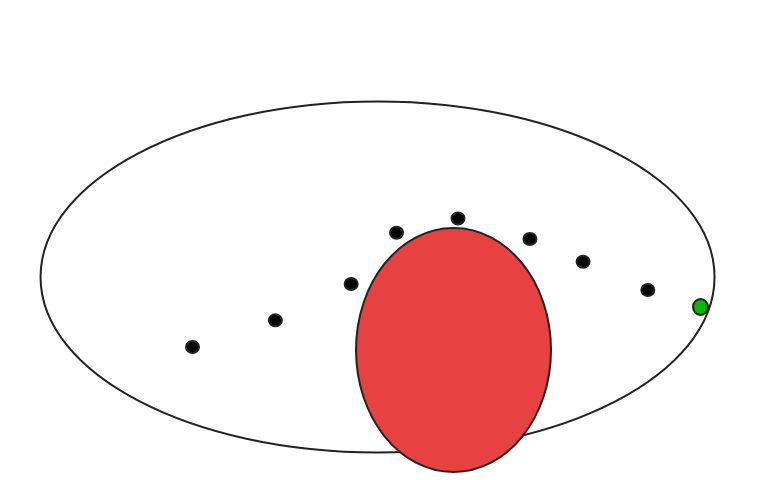
\includegraphics[width=200px]{images/infeasible_constraint.png}
% %\end{center}
% 
% If the runtime of the simulation depends on its inputs, and the simulation is not allowed to finish when a runtime threshold is met, the runtime will force some inputs to be infeasible.
% However, when the simulation does complete, its runtime is quantifiable, and can be used to construct a model of the infeasible region.
% An algorithm that wishes to minimize this simulation is forced to account for this constraint.
% 
% 
% An always feasible algorithm is also an \emph{any-time} algorithm.
% Anytime algorithms are a class of algorithms that can conveniently be run as long as desired and return the best solution found so far if interrupted.
% These algorithm are of practical importance when problems have uncertain time complexity.
% 


\section{Background}

\subsection{Notation}

Any variables that depend on the iteration will be super-scripted by $k$.
For example, the $k$-th iterate is given by $\xk$, and the model of the objective is given by $\mfk$.
The $i$-th row of the matrix $A$ is denoted $A_i$, while the $i$-th column is denoted $A_{\bullet i}$.
Subscripts on vectors are used as an index into the vector, while vectors in a sequence of vectors use superscripts.
Matrices are denoted with capital letters, and we use $e_i$ to denote the $i$-th unit vector.                     %, while sets are denoted with capital italic letters.

$B_k(c; \Delta)$ is the ball of radius $\Delta$ in the $k$ norm, centered at point $c$ .
$\delta_{i,j}$ is the kronecker delta, $\delta_{i,i} = 1$, $\delta_{i,j} = 0$ if $i\ne j$.


\subsection{Model-based Trust Region Methods}

We will modify the following derivative free trust region algorithm.
%A set of poised points are chosen for some radius $\Delta_k>0$ about the current iterate.
The objective value and derivatives are approximated in a trust region around the current iterate to construct their model functions.
Next, this model function is minimized over the trust region and the minimum argument becomes the trial point.
The objective is evaluated at the trial point and a measure of reduction $\rho$ is computed.
If $\rho$ implies that sufficient reduction has been made and that the model approximates the function well, the trial point is accepted as the new iterate.
Otherwise, the trust region is reduced to increase model accuracy.
The algorithm terminates when both and a criticality measure $\chik$ and the trust region radius $\Delta_k$ reach sufficiently small thresholds of $\tau_{\chi}$ and $\tau_{\Delta}$.


For unconstrained optimization, the algorithmic framework is described in \cref{unconstrained_dfo}.
% 	\begin {itemize}
%         \item The objective is evaluated at a set of sample point $Y$ to approximate $f$ \cref{interpolation}
%         \item Geometric properties ensure bounds on $f(x) - \mfk(x)$, $\nabla f(x) - \gradmodelk(x)$, and $\nabla^2 f(x) - \nabla^2\mfk(x)\;\forall x$ in the trust region \cref{geometry}
% 		%\[
% 		%\mfk(x) = f(\xk) + \nabla f(\xk)^T (x-\xk) + \frac 1 2 (x-\xk)^T\nabla^2f(\xk)(x-\xk)
% 		%\]
% 		\item If $\rho$ is large, $\xkpo=\xk+\trialk$ (accept) and either increase the radius or decrease if $\nabla \mfk(\xk)$ is small
% \end{itemize}

\begin{algorithm}[H]
    \caption{Unconstrained Derivative Free Algorithm}
    \label{unconstrained_dfo}
    \begin{itemize}
        \item[\textbf{Step 0}] \textbf{(Initialization)} \\
            Initialize tolerance constants $\tau_{\chi} \ge 0$, $\tau_{\Delta} \ge 0$, starting point $x^{(0)}$, initial radius $\Delta_0 > 0$, iteration counter $k=0$, and constants $\omegadec \in (0, 1)$, $ \gammasm \in (0, 1)$, $\gammabi \in (\gammasm, 1)$.
            
        \item[\textbf{Step 1}] \textbf{(Construct the model function)} \\
            Call the model improvement ``\cref{model_improving_algorithm}" to provide a set of sample points $Y^{(k)}$.
            Evaluate the objective on these points and use interpolation \cref{interpolation_formula} to construct the model function $\mfk(x)$.
        
        \item[\textbf{Step 2}] \textbf{(Check stopping criteria)} \\
            Compute the criticality measure $\chik$ such as $\chik = \|\nabla\mfk(\xk)\|$. \begin{itemize}
                \item[] If $ \chik < \tau_{\chi} $ and $\Delta_k<\tau_{\Delta}$ then return solution $\xk$.
                \item[] If $ \chik < \tau_{\chi} $ but $\Delta_k\ge\tau_{\Delta}$ then  
                set $\Delta_{k+1} \gets \omegadec\Delta_{k}$, 
                $x^{(k+1)} \gets \xk$,
                $k \gets k+1$ and go to Step 1.
            \end{itemize}
        
        \item[\textbf{Step 3}] \textbf{(Solve the trust region subproblem)} \\
            Compute $\trialk = \argmin_{s\in B_2(0; \Delta_k)} \mfk (\xk + s)$ where $B_2(0; \Delta_k)$ is the ball of radius $\Delta_k$ defined in \cref{tab:TableOfNotation}.
            
        \item[\textbf{Step 4}] \textbf{(Test for improvement)} \\
            Compute $\rho$ with \cref{rho} \begin{itemize}
                \item[] If $\rho < \gammasm$ then $\xkpo \gets \xk$ (reject) and $\Delta_{k+1} \gets \omegadec\Delta_{k}$
                \item[] If $\rho \ge \gammasm$ and $\rho < \gammabi$ then $\xkpo\gets\xk+\trialk$ (accept) $\Delta_{k+1} \gets \omegadec\Delta_{k}$
                \item[] If $\rho \ge \gammabi$ and $\|\trialk\| = \Delta_{k}$ then $\xkpo=\xk+\trialk$ (accept) $\Delta_{k+1} \gets \omegainc\Delta_{k}$
                % and either increase the radius or decrease if $\nabla \mfk(\xk)$ is small
            \end{itemize}
            $k \gets k+1$ and go to Step 1.
    \end{itemize}
\end{algorithm}

This derivative-free optimization algorithm differs from the classical trust region algorithm in two important respects:
\begin{enumerate}
    \item Models are constructed without derivative information.
    \item The trust region radius $\Delta_k$ must go to zero as $k\to\infty$.
\end{enumerate}

This is required to ensure that the gradient of the model function is equal to the gradient of $f$ in the limit.
Our goal is to generalize this framework to handle constraints, where we must ensure no constraint violation occurs while also ensuring the accuracy of the models of the constraints.
% Two challenges while adopting this framework to derivative free optimization are
% 
% Because explicit derivatives are not available, Taylor approximations cannot be used.
% The alternative to Taylor approximations that we employ is interpolation.
% Also, classical trust region methods do not require $\Delta_k \to 0$, but the bounds on model accuracy in derivative free optimization depend on the trust region radius.
% This means that in order to ensure $\nabla f < c\tau$ using the approximation  $\nabla \mfk < \tau$, the trust region must be sufficiently small.
%   
  

\section{Derivative Free Background}
% 
% \subsection{Strategy}
% A reasonable approach to DFO is to modify classical algorithms that rely on derivatives by using the derivatives of the model functions whenever a derivative is needed in the algorithm.
% However, the lack of explicit derivatives pose several challenges, which necessitate changes in the classical algorithms.
% First, care must be taken to ensure that the model functions are sufficiently accurate approximations to the true functions.
% This means that geometry of the sample points must be considered.
% It also means that the trust-region radius must get arbitrarily small.
% 
% The transition to the derivative-free setting also provides some interesting research opportunities.
% In particular, because function evaluations are so costly, there is potential for significant gains by considering more complex optimization paradigms.
% For example, Sequential Quadratic Programming (SQP) methods use subproblems involving quadratic approximations of the objective function $f$ and linear approximations of the constraint functions.
% In the derivative-free setting, it may be worthwhile to explore other variations of the classical algorithms.
% For example, it might be worthwhile to construct quadratic models of the constraint functions, which might result in fewer iterations overall.
% 
% It might also be worthwhile to consider using different sample sets for fitting different functions.  
% For example, the SQP trust-region filter method involves constructing a quadratic model of the objective function and linear models of the constraint functions.  But this raises an interesting question, since a good sample set for constructing a quadratic model may not be ideal for fitting the linear functions modeling the constraints.  

\subsection{Recent Work}
\paragraph{Applications}
Recently, there has been a growth in applications of derivative free optimization.
Such applications include photo-injector optimization \cite{1742-6596-874-1-012062}, circuitry arrangements \cite{PLOSKAS201816}, machine learning \cite{KS2018}, volume optimization \cite{Cheng2017}, and reliability based optimization \cite{Gao2017}.

\paragraph{Constrained derivative free algorithms}
To address the rise in these applications, new algorithms are being developed such as \cite{doi:10.1080/10556788.2015.1026968} which is an algorithm similar to the one presented here, but the sample points are not always feasible.
\cite{Troltzsch2016} presents another similar algorithm for equality based constraints.
\cite{infeasiblestarting} presents an algorithm which accepts an infeasible starting point.
\cite{Gao2018} also presents an algorithm for linearly constrained derivative free optimization that uses a backtracking technique to minimize the number of evaluations required.

\paragraph{Subproblems}
Some work has been done within trust region algorithms to improve the update policy \cite{Kamandi2017}.
Also, \cite{Verderio2017} and \cite{doi:10.1080/10556780802409296} discuss geometric conditions of the sample points required for global convergence.
Finally, \cite{AMAIOUA201813} uses a mesh adaptive search to solve quadratic subproblems.


\paragraph{Complexity Analysis}

A derivation is found in \cite{doi:10.1137/151005683} which shows that to driver the norm of the gradient less than $\epsilon$, the number of function evaluations can be bounded by $O(\epsilon^{-2})$ 
%and $O(n^2\epsilon^{-2})$ 
function evaluations for derivative free model based approaches. Also, cubic over estimation with finite differences can acheive $O(\epsilon^{-1.5})$. \cite{doi:10.1093/imanum/drx043} is another recent paper presenting complexity analysis using probabilistic methods.


\paragraph{Reviews}
Within \cite{DUMMY:intro_book} derivative-free methods are developed in detail.
This is the first text book devoted to derivative free optimization.
It contains a good explanation of ensuring geometry of the current set with poisedness for unconstrained problems and also covers other derivative-free methods including direct-search and line search.

A good review of derivative free algorithms and software libraries can be found in \cite{DUMMY:review}.
This compares several software libraries, and reviews the development of derivative free optimization since it started.
Another recent review can be found in \cite{DUMMY:review2} and \cite{Larson_2019}.

% TODOOOOOOOOOOOOOOOOOOOOOOOOOOOOOOOOOOOOOOOOOOOOOOOOOOOOOOOOOOOOOOOOOOOOOOOOOOOOOOOOOOOOOOOOOOOOOOOOOOOOOOOOOOOO
% READ THIS


\subsection{Sample Set Geometry}
\subsubsection{Interpolation}
\label{interpolation}

Derivative free trust region methods construct model functions from a family of functions spanned by a set of $p + 1 \in \naturals$ basis functions  $\{\phi_0, \phi_1, \ldots, \phi_p\}$.
Each member of this family has the from $\mfk(x) = \sum_{i=0}^p\alpha_i\phi_i(x)$ for some scalar coefficients $\alpha_i, i \in \{0, \ldots, p\}$.

In our method, we use interpolation to choose the coefficients so that $\mfk$ agrees with $f$ on a set of $p+1$ sample points $Y = \{y^0, y^1, \ldots, y^p\}$ for which the functions have been evaluated.
Thus the model functions must satisfy:
\begin{align}
\label{interpolation_condition}
\mfk(y^i) = f(y^i) \quad \forall \quad 0 \le i \le p.
\end{align}
This is known as the \emph{interpolation condition}.

To satisfy the interpolation condition \cref{interpolation_condition}, we then chose this linear combination by selecting coefficients $\alpha_0, \ldots, \alpha_p$ to satisfy
\begin{align}
\label{interpolation_formula}
    \mfk(y^i) = \sum^p_{j=0}\alpha_j\phi_j(y^i) = f(y^i) \quad \forall \quad 0 \le i \le p.
\end{align}

% We can also write this equation in matrix form.
If we define the Vandermode matrix as
\begin{align}
\label{vandermonde}
V=
\begin{bmatrix}
    \phi_0(y^0)      & \phi_1(y^0)       & \ldots & \phi_{p}(y^0)      \\
    \phi_0(y^1)      & \phi_1(y^1)       & \dots  & \phi_{p}(y^1)      \\
                     &                   & \vdots &                    \\
    \phi_0(y^{p})    & \phi_1(y^{p})     & \ldots & \phi_{p}(y^{p})
\end{bmatrix},
\end{align}

the interpolation condition becomes:
\begin{align}
\label{matrix_form}
V
\begin{bmatrix}
    \alpha_0     \\
    \alpha_1     \\
    \vdots       \\
    \alpha_p
\end{bmatrix}
=
\begin{bmatrix}
    f(y^0)     \\
    f(y^1)     \\
    \vdots     \\
    f(y^p)
\end{bmatrix}
\end{align}

% Suppose that we use $p+1$ sample points $Y = \{y^0, y^1, \ldots, y^p\}$ to construct the approximation of $f$.
We desire a method for choosing these sample points that provides error bounds on not only the function values, but also on orders of derivatives in some region around the current iterate.
% The model is constructed to agree with the original functions on at least the sample points: we evaluate the objective here, so that we know the true function values at these points.
% For the objective, this becomes

%It is convenient to write the model as a linear combination of basis polynomials $\{\phi_0, \phi_2, \ldots, \phi_p\}$.


\subsubsection{Geometry}
\label{geometry}
The term \emph{geometry} describes how the distribution of points in the sample set $Y$ affects the model's accuracy.
\cref{matrix_form} has a unique solution if and only if $V$ is nonsingular, in this case, we say that the sample set $Y$ is \emph{poised} for interpolation with respect to the basis functions $\phi_i$.
However, even when $V$ is nonsingular but ``close" to singular, as measured by its condition number, the model's approximation may become inaccurate.
% The condition number of $V$ measures how far the current Vandermode matrix is from being illpoised.
Algorithms must be careful to avoid choices of sample points $Y$ that cause the condition number of this matrix to be too large.

In the case of polynomial model functions, a careful analysis of model accuracy can be performed using \emph{Lagrange polynomials}.
Let the space of polynomials with degree less than or equal to $d$ be denoted $\polydn$ and have dimension $p+1$.
The Lagrange polynomials $l_0, l_1, \ldots, l_p$ for the sample set $Y$ are a basis of $\polydn$ such that
\begin{align}
l_i(y^j) = \delta_{i,j}
\end{align}
where $\delta_{i,j} = \{0 \;\text{if}\; i\ne j,\quad 1 \;\text{if} \; i = j \}$ is the Kronecker-delta function.
%For example, after this change of basis, note that the Vandermonde matrix becomes the identity matrix.
Thus, we can conveniently write
\begin{align}
\label{reg}
\mfk(x) = \sum^p_{j=0}f(y^i)l_i(x).
\end{align}
%This implies computing the change of basis to the Lagrange polynomials amounts to inverting this Vandermonde matrix.
%This relationship allows us to use properties of the Vandermonde matrix and these Lagrange polynomials to find conditions on our sample points that ensure nice geometry.

We say that a set $Y$ is \emph{$\Lambda$-poised} for a fixed constant $\Lambda$ with respect to a bases $\phi$ on the set 
$B \subset\Rn$ if and only if for the Lagrange polynomials $l_i$ associated with $Y$
\begin{align}
\Lambda \ge \max_{0\le i\le p}\max_{x\in B}|l_i(x)|.
\end{align}

% This can be shown to be equivalent to the following condition \cite{DUMMY:intro_book}.
% For any $x \in B_2(0, 1)$ there is a $\lambda \in \reals ^ {p+1}$ such that 
% \begin{align}
% \sum_{i=0}^p\lambda_i\phi_i(y^i) = \phi(x) \\
% \|\lambda\|_{\infty} \le \Lambda.
% \end{align}

% This can ensure that the Vandermonde matrix is well conditioned.
This is useful because of the following results found in \cite{DUMMY:intro_book}.



\begin{assumption}
\label{fully_quadratic_assumption}
Suppose that a set $S$ and a radius $\dmax$ are given.
Assume that $f$ is twice continuously differentiable with Lipshcitz continuous Hessian in an open domain containing the $\dmax$ neighborhood
$\cup_{x \in S} B(x; \dmax)$ of the set $S$.
\end{assumption}

\begin{definition}
\label{fully_quadratic_definition}
Let $f$ be a function that satisfies \cref{fully_quadratic_assumption}.
For any $\Delta \in (0, \dmax)$ and $x \in S$, a model function $m : \Rn \to\reals, m \in C^2$ with Lipschitz continuous Hessian with corresponding Lipschitz constant bounded by $\nu_2$  is called a fully quadratic if there exist positive constants
$\kappa_f$, $\kappa_g$, and $\kappa_h$ such that:
\begin{align}
\|\nabla^2 f(y) - \nabla^2 m(y)\| \le \kappa_{h} \Delta \quad \forall y \in B_2(x; \Delta) \label{error_in_hessian}\\
\|\nabla f(y) - \nabla m(y)\| \le \kappa_{g} \Delta^2 \quad \forall y \in B_2(x; \Delta) \label{error_in_gradient} \\
|f(y) - m(y) | \le \kappa_{f} \Delta^3 \quad \forall y \in B_2(x; \Delta). \label{error_in_function} 
\end{align}
\end{definition}

% Assuming that $f$ is twice continuously differentiable in an open domain containing $B_2(y^0, \Delta)$ and has a Lipschitz continuous Hessian, using quadratic interpolation there exist constants $\kappa_{ef}, \kappa_{eg}$, and $\kappa_{eh}$ depending only on the dimension and Lipschitz constant of $\nabla^2 f$ such that for any $y \in B_2(y^0, \Delta)$ :
% \begin{align}
%  \|f(y) - \mfk(y)\| \le \kappa_{ef} \Lambda \Delta^3 \\
%  \|\nabla f(y) - \nabla \mfk(y)\| \le \kappa_{eg} \Lambda \Delta^2 \\
%  \|\nabla^2 f(y) - \nabla^2 \mfk(y)\| \le \kappa_{eh}\Lambda \Delta .\\
% \end{align}
Also, \cite{DUMMY:intro_book} also shows that ensuring a bound on the condition number of the Vandermonde matrix ensures $\Lambda$-poisedness.

In particular, these bounds ensure that the following accuracy condition is satisfied, which is used by \cite{Conejo:2013:GCT:2620806.2621814} to prove convergence to a first order critical point: 
\begin{equation}
\label{accuracy}
\|\nabla \mfk(\xk) - \nabla f(\xk) \| \le \kappa_g \Delta_k
\end{equation}
 for some fixed constant $\kappa_g$ independent of $k$.
We will extend these results for ellipsoidal trust regions in \cref{ellipsoidal_lambda}.
 

%used to find the coefficients $\lambda$ to express the model function in terms of a basis of Lagrange polynomials $l_i$
The following example illustrates how interpolating with an ill-poised set can produce an inaccurate model.
% Problems become apparent when comparing the Lagrange polynomials associated with a poised set with those of an ill poised set.
In \cref{pvip}, a set of quadratic polynomials is used to interpolate the function $f(x) = 5 + x + y + (x + y) ^ 2 - \frac 1 {250} y ^ 4$.
We can see that the difference between the model and $f$ are much larger when the points are chosen to be nearly collinear.
This results in a much higher $\Lambda$.

\begin{figure}[h]
    \centering
    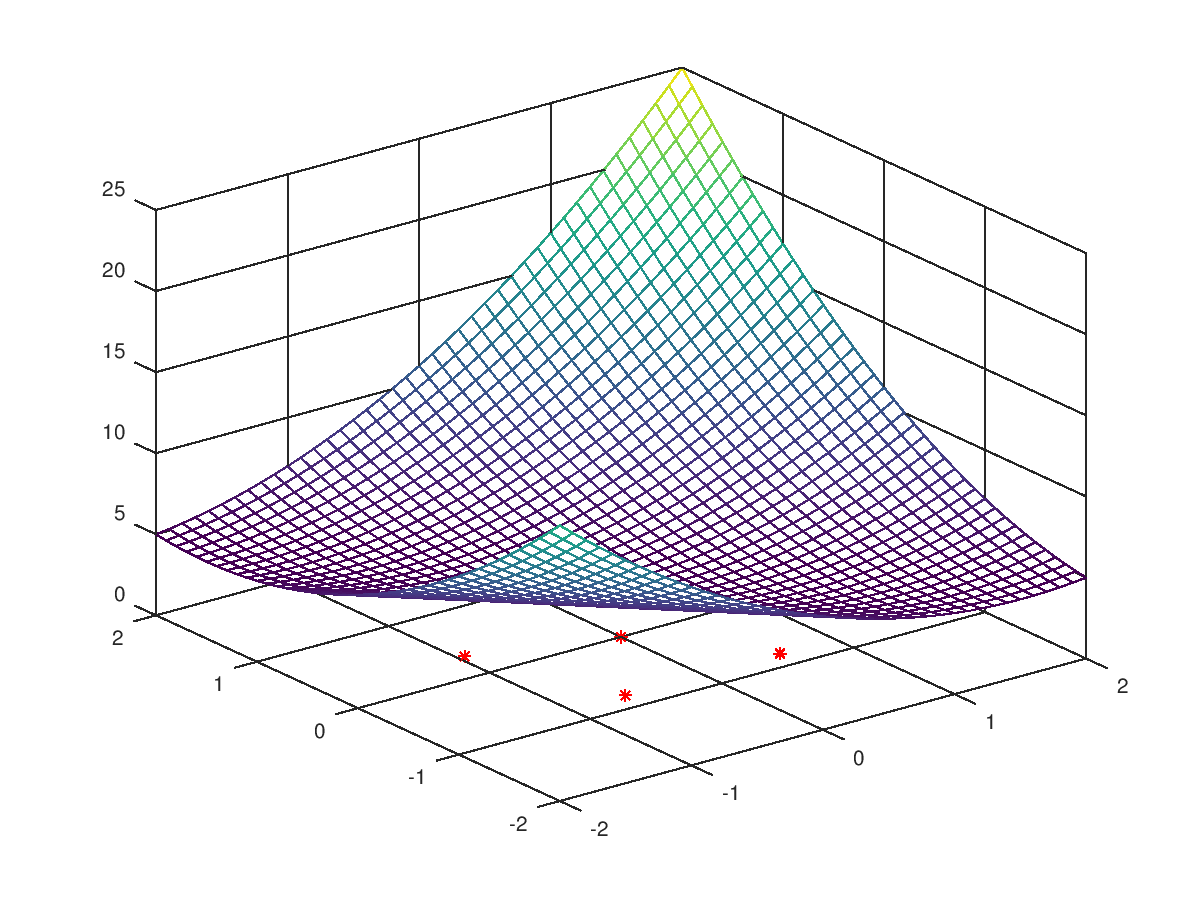
\includegraphics[width=200px]{images/poised_good.png}
    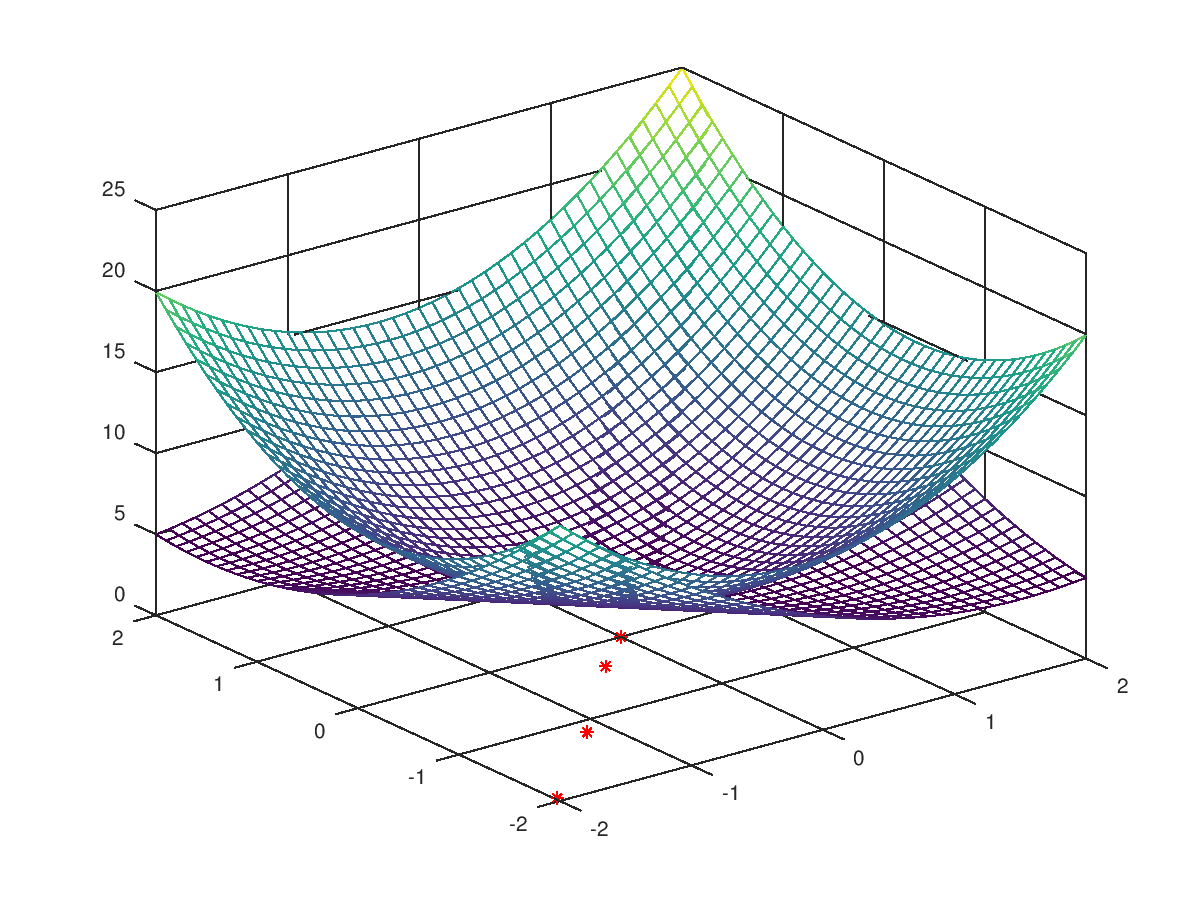
\includegraphics[width=200px]{images/poised_bad.png}
    \caption{
		Poised vs Ill poised.
		On the left, a well poised sample set is used and the model is indistinguishable from the true function.
		On the right, the sample set has poor geometry, and the model goes above the true function.
	}
    \label{pvip}
\end{figure}


A more detailed discussion can be found in \cite{doi:10.1080/10556780802409296}, but a step to ensure good geometry is required for convergence analysis although it may come at the expense of adding more function evaluations.

\subsubsection{Geometry Ensuring Algorithms}

Sample points are chosen by a geometry ensuring algorithm from \cite{DUMMY:intro_book}.
At any given time, the algorithm has evaluated 1 or more sample points.
Initially, only the starting point $x_0$ is evaluated, so that points must be added to the sample set.
Evaluated points within the trust region should be reused when possible, but the algorithm may have to replace some points to ensure a well poised set on the new trust region.
We call the algorithm that adds points, replacing where necessary, the \emph{model improvement algorithm}.
One classic such algorithm is presented in \cite{DUMMY:intro_book}.

The idea behind this algorithm is to perform an LU factorization with partial pivoting on the Vandermonde matrix.
As we have seen, this computes the basis for the Lagrange polynomials corresponding to $Y$.
However, when this LU factorization encounters a small pivot, the point corresponding to that row is replaced, improving the condition number of the Vandermonde matrix.

In practice, we first shift the sample set $Y$ by subtracting the current iterate and dividing by the trust region radius:
\begin{align}
\bar{Y} = [0, \frac{y^1 - y^0}{\Delta}, \ldots, \frac{y^p - y^0}{\Delta}]
\end{align}

At times, the algorithm will not have all $p+1$ points.
This can be because it is only given one point during initialization, or because points not within the trust region are removed.
Because the model improvement algorithm requires all $p+1$ points, we initialize $y^i = y^0$ for any $0 < i \le p$ corresponding to a missing point.
We choose a threshold $0 < \ximin < 1$, and follow \cref{model_improving_algorithm}:

\begin{algorithm}[H]
    \caption{Model Improvement Algorithm}
    \label{model_improving_algorithm}
    \begin{itemize}
        \item[\textbf{Step 0}] \textbf{(Initialization)} \\
            Initialize $i=1$.
            Given a non-empty set $Y$ of $p+1$ points. 
            Construct the Vandermonde matrix $V_{i,j} = \phi_j(\frac 1 {\Delta}(y^i - y^0))$.
			Initialize constant $\ximin > 0$.
        \item[\textbf{Step 1}] \textbf{(Pivot)} \\
            Swap row $i$ with row $i_{\max} = \arg \max_{j|j\ge i} V_{j,i} $
        
        \item[\textbf{Step 2}] \textbf{(Check threshold)} \begin{itemize}
                \item[] If $|V_{i,i}| < \ximin$ then select \label{next_point} $\hat y \in \argmax_{t | \|t\|\le 1} |\phi_i(t)|$
                \item[] Replace row $i$ with $V_{i, j} \gets \phi_j(\hat y)$.
            \end{itemize}
        
        \item[\textbf{Step 3}] \textbf{(LU)} \begin{itemize}
                \item[] Set $V_i \gets \frac{1}{V_{i,i}} V_i$
                \item[] Set $V_{\bullet j} \gets V_{\bullet j} - V_{i,j} V_{\bullet j} \forall j=i \ldots p$
            \end{itemize}
            If $i = p$ then \textbf{Stop}, otherwise Set $i \gets i+1$ and go to Step 1
    \end{itemize}
\end{algorithm}


At the end of this algorithm, the points in $Y$ will be $\Lambda$-poised for some $\Lambda$ depending on the constant $\xi_{min}$.
The following result is shown in \cite{DUMMY:intro_book}.
\begin{theorem}
\label{set_is_fully_quadratic}
Let $f$ satisfy \cref{fully_quadratic_assumption}.
For any $\epsilon \in (0, \frac 1 4)$, and $p+1 = \frac {(n+1)(n+2)}{2}$, \cref{model_improving_algorithm} produces a set of $p+1$ points in the unit ball $B(0; 1)$ such that if $m_f$ is the Lagrange-interpolating model of $f$ given by \cref{reg}, then the $m_f$ is fully a quadratic model.
\end{theorem}

This algorithm can also be used to create a poised set over an ellipsoidal shape. This is discussed further in \cref{ellipsoidal_lambda}.
% 
% \paragraph{Proximity}
% 
% Proximity refers to the trust region radius.
% The trust region must go to zero if we are to be sure we have reached a critical point.
% In general, the smaller the trust region, the closer to linear or quadratic the original function will look.
% This is because the model's error term is proportional to the trust region radius.
% 
% In classical trust region algorithms, there is no need for the trust region radius to go to zero.
% Therefore, extra care must be taken to ensure this while modifying such algorithms.


\subsection{Algorithm Components}

We will discuss several building blocks of the algorithm before going into the algorithm's detail.

\subsubsection{Criticality Measure}

In order to define stopping criteria for the algorithm, we introduce a criticality measure $\chi$ which goes to zero as the iterates approach a first order critical point.
When the criticality measure is small, we must also decrease the trust region radius.
Once this has reached a small enough threshold $\tau_{\chi}$ and the trust region is small enough ($\Delta_k < \tau_{\Delta}$), we can terminate the algorithm.
For now, our algorithm is designed to work with convex constraints, so we employ a classic criticality measure discussed in \cite{ConnGoulToin00} of

\begin{align*}
\chik = \|\xk - \text{Proj}_{\feasiblek}(\xk- \nabla \mfk(\xk))\|
\end{align*}

where $\feasiblek$ denotes the feasible region: $\feasiblek = \{x \in X | \mcik(x) \le 0 \quad \forall 1 \le i \le m \}$.
This criticality measure measures how far the current is from satisfying the first order optimality conditions for $\xk$ to be a constrained minimum of $\mfk$.
When $ \lim_{k\to\infty} \chik = 0$, $\lim_{k\to\infty}\Delta_k = 0$, and $\lim_{k\to\infty}\xk = x^{\star}$, then we have that $x^{\star}$ also satisfies the first order optimality conditions of being a constrained minimum of $f$.

%we have $x = \text{Proj}_{\feasiblek}(x - \nabla \mfk(x))$ so that

$\chik$ can be computed as 
\begin{align}
\label{critical}
\trialk = \min_{s \in \feasiblek} \|\xk - \nabla \mfk(\xk) - s\|^2 \\
\chik = \|\xk - \trialk \|^2 \\
\end{align}

% This remains large while there is feasible search space along a descent direction, but small otherwise or if the gradient goes to zero.

% Namely, when $ \chik(x) = 0$, we have $x = \text{Proj}_{\feasiblek}(x - \nabla \mfk(x))$ so that there is no decent direction along $\nabla \mfk(x)$ as it points away from the feasible region.
% As $\Delta_k$ gets smaller, we also have that $\mfk$ better represents $\nabla f$, so that $\nabla f$ will also either be zero or lie in the iterate's normal cone.

\subsubsection{Assessing Model Accuracy and Radius Management}

Each iteration that evaluates a trial point must also test the accuracy of the model functions.
To test the accuracy, we calculate a quantity
\begin{equation}
\label{rho}
\rho_k = \frac{f(\xk) - f(\xk+\trialk)}{\mfk(\xk) - \mfk(\xk+\trialk)}
\end{equation}
which measures the actual improvement over the predicted improvement.
A small $\rho_k$ implies the model functions are not sufficiently accurate.
Values of $\rho_k$ close to $1$ imply that the model accurately predicted the new objective value.
A large $\rho_k$ implies progress minimizing the objective although the model was not accurate.
This has been widely used within trust region frameworks such as \cite{Conn:2000:TM:357813} and within a derivative free context \cite{DUMMY:intro_book}.
The user supplies fixed constants $0 < \gammasm \le \gammabi \le 1$ as thresholds on $\rho_k$ and $0 < \omega_{\text{dec}} < 1 \le \omega_{\text{inc}}$ as decrement or increment factors to determine the trust region update policy.
The update policy frequently follows Step 4 within algorithm \cref{unconstrained_dfo} repeated within \cref{trust_region_update} for ease.

\begin{algorithm}[H]
    \caption{Trust Region Update Policy}
    \label{trust_region_update}
    \begin{itemize}
        \item[\textbf{Step 4}] \textbf{(Test for improvement)} \\
            Compute $\rho_k$ with \cref{rho} \begin{itemize}
                \item[] If $\rho_k < \gammasm$ then set $\xkpo \gets \xk$ (reject) and $\Delta_{k+1} \gets \omegadec\Delta_{k}$
                \item[] If $\rho_k \ge \gammasm$ and $\rho < \gammabi$ then set $\xkpo\gets\xk+\trialk$ (accept) and $\Delta_{k+1} \gets \omegadec\Delta_{k}$
                \item[] If $\rho_k \ge \gammabi$ and $\|\trialk\| = \Delta_{k}$ then set $\xkpo=\xk+\trialk$ (accept) and $\Delta_{k+1} \gets \omegainc\Delta_{k}$
                % and either increase the radius or decrease if $\nabla \mfk(\xk)$ is small
            \end{itemize}
            $k \gets k+1$ and go to Step 1.
    \end{itemize}
\end{algorithm}

\subsubsection{Sufficient Model Reduction}

To ensure sufficient reduction of the objective's model function during each iteration, we impose the following efficiency condition:
\begin{equation}
\label{efficiency}
\mfk(\xk) - \mfk(\xk + \trialk) \ge \kappa_f \chi_k \min\left\{ \frac{\chi_k}{1+\|\nabla^2 \mfk(\xk)\|}, \dk, 1 \right\}
\end{equation}
where $\kappa_f$ is a constant independent of $k$.
This is widely used within trust region frameworks such as \cite{Conejo:2013:GCT:2620806.2621814} and \cite{Conn:2000:TM:357813}.
It can be shown that the \emph{generalized Cauchy point} satisfies this condition \cite{Conn:2000:TM:357813}.


\subsubsection{Trust Regions}
Our algorithm maintains up to three trust regions.
The outer trust region is an $L_1$ ball of radius $ \dk $ defined by
\begin{equation}
\label{trust_region}
\outertrk = B_{\infty}(\xk,\dk) = \{x\in \Rn | \; {\xk}_i - \dk \le x_i \le {\xk}_i + \dk \quad \forall 1\le i \le n\}.
\end{equation}

Note that the outer trust region may include infeasible points.
To ensure feasibility of all sample points, we construct an inner trust region for sample points $ \sampletrk $  satisfying 
$\sampletrk \subset \outertrk \cap \feasiblek$ and $\xk \in \sampletrk $.
However, we do not want to limit the search for a new iterate to the same trust region we use to construct the model.
This means we introduce another trust region $ \searchtrk $ that also satisfies $ \searchtrk \subset \outertrk \cap \feasiblek$ and $\xk \in \searchtrk $ for the trust region subproblem.

\paragraph{The Sample Region}
\label{sample_region_choices}
We consider general strategies for constructing $ \sampletrk $ and $ \searchtrk $.
\begin{itemize}
\item[1.] Take 
\begin{align}
\label{redpill} \sampletrk = \searchtrk = \outertrk \cap \feasiblek.
\end{align} This results in a polyhedral trust region, so we refer to this approach as the \emph{Polyhedral Trust Region Approach}.
% \item[2.] Let $\label{hybrid} \sampletrk \subseteq \searchtrk = \outertrk \cap \feasiblek $ where $\sampletrk$ has an ellipsoidal shape. This is referred to as the \emph{Hyrbid Trust Region Approach}
\item[2.] Force 
\begin{align}\label{bluepill} \sampletrk \subseteq \searchtrk \subseteq \outertrk \cap \feasiblek
\end{align} where $\sampletrk$ has an ellipsoidal shape. This is referred to as the \emph{Ellipsoidal Trust Region Approach}
\end{itemize}

The advantage of the ellipsoidal trust region approach \cref{bluepill} is that we can reuse classical methods for ensuring good geometry.
We can construct $\sampletrk$ to be ellipsoidal and use efficient algorithms within \cite{DUMMY:intro_book} to satisfy \cref{accuracy}.
However, we must be careful while choosing $ \searchtrk$ to allow sufficient reduction when we solve the trust region subproblem using the inner trust region.
The search trust region is used while selecting the next iterate:
\begin{align*}
\trialk = \argmin_{\trialk \in \searchtrk} \mfk(\xk + \trialk)
\end{align*}

\paragraph{The Search Region}
\label{search_region_choices}
When using the ellipsoidal trust region approach, we have two choices for this trust region:
\begin{align}
\searchtrk = \sampletrk \label{search_a_little}
\end{align}
\begin{align}
\searchtrk = \outertrk \cap \feasiblek \label{search_a_lot}
\end{align}
Namely, in \cref{search_a_little} with an ellipsoidal inner trust region, we still have an option to select our trial point from the entire $\trialk \in \outertrk \cap \feasiblek$.

To complete the polyhedral trust region approach \cref{redpill}, %$\innertrk = \outertrk \cap \feasiblek$
, we need some redefinition of poisedness for polyhedral shapes.
However, since the trust region is larger, it is easier to ensure sufficient reduction.
This strategy has the drawback that it will yield sample points close to the boundary of the feasible region.
This may cause more infeasible evaluation attempts when we use models to approximate black-box constraints this may.

The classical methods for ensuring good geometry require an optimization call to the model functions over a sphere.
This is no longer possible in the polyhedral trust region approach.
However, the bounds produced over the entire trust region may also be stronger than required as the models will only be used on the feasible region.
This may mean the geometric requirements can be reduced.
Looking again at the ill-poised set in \cref{aoip}, the set of nearly collinear sample points actually does appear to be accurate over a smaller trust region.


\begin{figure}[h]
    \centering
    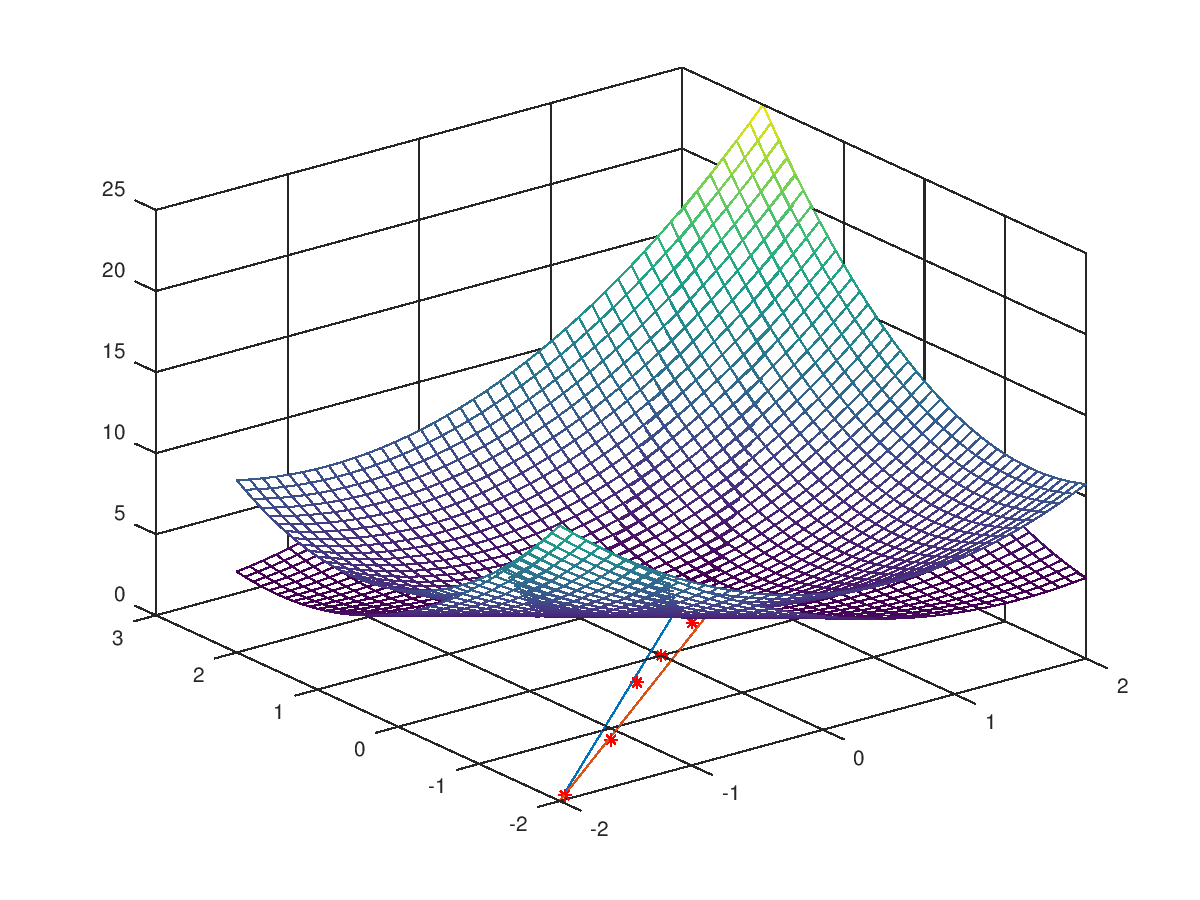
\includegraphics[width=200px]{images/poised_bad_but_good.png}
    \caption{Accurate model over thin trust region from illpoised set}
    \label{aoip}
\end{figure}


Within our algorithm, if $ \outertrk \subseteq \feasiblek$ we can set $ \sampletrk $ to be a sphere.
This saves the computation of $ \sampletrk $ when it is not needed, as there are no nearby constraints.




% \paragraph{}
% While including a center search and only using a sphere for $\sampletrk$ ensures that this will be the case as long as there is an interior point to the feasible region.
% However, for more complicated ellipsoid searches must be able to find an ellipse.
% One strategy that ensures the ellipse can be constructed for all of our ellipse searches is to find an ball containing the current iterate and running a local search optimization routine with this initial ball as input.


% 
% \paragraph{}
% Another strategy is to add a check within the \emph{ConstructTrustRegion} routine that decreases the trust region radius whenever a suitable ellipse is not found.
% The presented convergence analysis will still hold as $S$ can contain only finitely many terms not in $\bar S$.

% \paragraph{}
% \color{red}
% For convex constraints, there will exist a bound on the condition numer of $\qk$ as long as $\outertrk$ is bounded.
% An argument for this might be as follows:
% Maybe, by increasing the outer trust region radius, we can only increase the condition number of $\qk$.
% \color{black}




\chapter{Background}\label{chap:background}
% Within this chapter, we discuss background material relevant to our algorithm.
% This begins with a brief review of the literature within \cref{literature_review}.
% We then discuss our criticality measure $\xi$ and model accuracy $\rho$ within \cref{criticality_measure_section} and \cref{rhosection}.
% The next sections \cref{interpolation}, \cref{geometry}, and \cref{model_improvement_algorithms} are devoted to developing background material for interpolation based methods.
% Finally, in \cref{trust_regions_section} we end with a discussion of trust regions, which we place in the context of our algorithm.



\section{Literature Review}

\label{literature_review}


% Recently, there has been a growth in applications of derivative-free optimization.
% Such applications include

% Model based, trust region, I think no constraints, maybe multi-objective:
% photo-injector optimization \cite{Neveu2017}.

% Direct search, binary constraints, mixed integer (nomad, midaco, glcSolve, CMAES (stochastic))
% circuitry arrangements \cite{PLOSKAS201816},

% For paralellizable methods, kalman filter methods, optimizing networks
% machine learning \cite{KS2018}

% Trust region based, reliability surrogate constraints
% and reliability based optimization \cite{Gao2017}.

% parallel algorim, compares gradient based and dfo, nelder-mead
% volume optimization \cite{Cheng2017},

Several books and survey articles  provide good introductions to the field of derivative-free optimization.
Within \cite{introduction_book}, derivative-free methods are developed in detail.
This is the first textbook devoted to derivative-free optimization.
It contains an explanation of how to ensure good sample set geometry and introduces the concept of 
poisedness for unconstrained problems, and it also covers other direct-search and line-search methods.   A review of derivative-free algorithms and software libraries can be found in \cite{miguel_review}.
This compares several software libraries and reviews the development of derivative-free optimization since it started.
Other recent reviews can be found in \cite{custodio_review2} and \cite{larson_menickelly_wild_2019}.

Most  algorithms for derivative-free optimization fall into two main categories: direct-search methods and model-based methods.   Direct-search methods use comparatively simple strategies to explore the solution space, using only the relative ranks of function values rather than their numerical values.     Early direct search methods for unconstrained optimization include coordinate descent \cite{fermi.metropolis:numerical},  the Nelder-Mead algorithm \cite{10.1093/comjnl/7.4.308},  
and pattern search methods \cite {hooke.jeeves:direct, kolda.lewis.ea:optimization}.   Generalizations of pattern-search methods include the GPS method \cite{torczon:convergence, Audet2002AnalysisOG} and the mesh adaptive direct search (MADS) algorithm \cite{audet.dennis:mesh, abramson.audet:convergence}.

Model-based methods guide the search using surrogate models of the black-box functions, which are constructed by fitting function values on a set of sample points.    Among the more commonly used model functions are linear and quadratic interpolation models \cite{ conn.scheinberg.ea:recent, powell:uobyqa,powell:newuoa}  and radial-basis function interpolation models \cite{oeuvray.bierlaire:boosters,wild.regis.ea:orbit,wild.shoemaker:global}.

The use of model functions allows curvature information to be incorporated into the search.  As such, model-based methods tend to be more efficient than direct-search methods when the black box functions are smooth.  In contrast, direct-search methods can be better suited for handling nonsmooth or noisy functions.   They are also more straightforward to implement, and are easier to parallelize.

Hybrid methods, which incorporate ideas from both direct-search and model-based methods, have also been proposed.    Some examples are described in \cite{booker.dennis.ea:rigorous}, \cite{thi.vaz.ea:optimizing}, and \cite{custodio.vicente:using}.

\paragraph*{Constrained derivative-free algorithms.}
To discuss methods for constrained derivative-free optimization,  we follow the constraint taxonomy      
of Le~Digabel and Wild \cite{ledigabel2015taxonomy} and distinguish between whether constraints are {\em relaxable} or {\em unrelaxable}.    An unrelaxable constraint is one that {\em must} be satisfied in order to obtain meaningful information about the objective function and/or constraint functions.    Thus algorithms for unrelaxable constraints can use function evaluations only for feasible points.   We also distinguish between whether constraints are {\em algebraic} or {\em black-box}.    A constraint is algebraic if the constraint functions can be computed algebraically,  whereas a {\em black-box constraint} can only be evaluated by running simulation software.    

\paragraph*{Relaxable constraints.}   The easiest class of constraints to deal with are the relaxable algebraic constraints.   In this case, ideas from classical nonlinear programming methods can easily be adapted to the derivative-free setting.  Some examples include 
 penalty methods \cite{lewis.torczon:globally, lewis.torczon:direct, bueno.friedlander.ea:inexact},   and filter methods \cite{brekelmans.driessen.ea:constrained, ferreira.karas.ea:global}.     
Both penalty methods and filter methods allow iterates to violate constraints, requiring feasibility only in the limit.  As such, they are viable approaches only when the constraints are relaxable.    
 
For relaxable black-box constraints,  several methods have been proposed that allow the black-box functions to be evaluated at infeasible points.  These include penalty methods
\cite{audet.dennis:progressive, liuzzi.lucidi:derivative-free, liuzzi.lucidi.ea:sequential,fasano.liuzzi.ea:linesearch,diniz-ehrhardt.martinez.ea:derivative-free,picheny2016bayesian}, filter methods \cite{audet.dennis:pattern, pourmohamad:combining,echebest.schuverdt.ea:inexact},  and funnel methods \cite{sampaio.toint:derivative-free,sampaio.toint:numerical}.

Another approach is to construct algebraic models of the constraint functions and then require iterates to be feasible with respect to these modelled constraints.
In \cite{glass.cooper:sequential},  linear models of nearly active constraint functions are constructed and the iterates are accepted only if they are feasible with respect to these modeled constraints.     A similar strategy is employed in the COBYLA method of Powell \cite{powell:direct}, which builds linear models of the objective and constraint functions based on a common set of sample points.    
A variant of the MADS algorithm is proposed in \cite{burmen.olensek.ea:mesh} which uses linear regression models of the constraint functions to guide the choice of search and poll steps.   In \cite{Troltzsch2016},  the classic sequential quadratic programming algorithm is implemented for equality-based constraints.




%Also, \cite{Gao2018} presents  an algorithm for linearly constrained derivative-free optimization that uses a backtracking technique to minimize the number of evaluations required.



\paragraph*{Unrelaxable algebraic constraints.}  

 An algebraic constraint function can always be evaluated, so the only way it is considered unrelaxable is if a black-box function (either the objective or some other constraint function) cannot be evaluated when the constraint is violated.
Note that it is always possible to determine whether a point satisfies an algebraic constraint prior to attempting to evaluate any black-box functions.  As such, it is relatively straightforward to modify direct-search methods to guarantee that only feasible points are considered.     
Many direct-search methods have been proposed that take this approach
\cite{box:new, spendley.hext.ea:sequential,may:linearly,may:solving,lewis.torczon:globally,lewis.torczon:direct,
vandenberghen:condor, lewis.torczon:pattern2000,lucidi.sciandrone:derivative-free,chandramouli.narayanan:scaled,kolda.lewis.ea:stationarity,lucidi.sciandrone.ea:objective, 
audet.ledigabel.ea:linear,gratton.royer.ea:direct2019,gratton.royer.ea:direct2015}
%
% \cite{box:new} \cite{spendley.hext.ea:sequential}, \cite{may:linearly}, \cite{may:solving},\cite{lewis.torczon:globally},  \cite{lewis.torczon:direct}, \cite{vandenberghen:condor}, \cite{lewis.torczon:pattern2000} \cite{lucidi.sciandrone:derivative-free}, \cite{chandramouli.narayanan:scaled},  \cite{kolda.lewis.ea:stationarity}, \cite{lucidi.sciandrone.ea:objective}, 
%\cite{audet.ledigabel.ea:linear},\cite{gratton.royer.ea:direct2019}, \cite{gratton.royer.ea:direct2015}
  
Developing model-based algorithms for unrelaxable constraints is complicated by the fact that the choice of sample points impacts the accuracy of the model functions.     Thus, when restrictions on the choice of sample points are imposed,  it can be difficult to ensure that the model functions are sufficiently accurate to guarantee convergence to a stationary point.    (see \cref{sec:polyhedral} for a more detailed explanation of this difficulty).   In the case of unrelaxable bound constraints, the restrictions on the sample points are not too difficult to mitigate.     The BOBYQA algorithm \cite{powell:BOBYQA} ensures that all points at which the objective function are evaluated satisfy the bound constraints, while still maintaining sufficient model accuracy to guarantee convergence.    In \cite{arouxet.echebest.ea:active-set},  an active set method is used when solving the bound-constrained trust-region subproblems.    In \cite{wild:derivative-free}, Wild proposed a radial basis function method for bound constraints, which enforces the bounds when selecting sample points in the model improvement algorithm and when solving the trust region subproblems.   In \cite{gratton.toint.ea:active-set}, Gratton et al. present a method which restricts the construction of the model functions to subspaces defined by nearly active bound constraints.

There has also been some progress in developing model-based methods for unrelaxable linear constraints.   In  \cite{gumma.hashim.ea:derivative-free},  Gumma et al.  propose the LCOBYQA algorithm which is an extension of Powell's NEWUOA algorithm that enforces the linear constraints both when solving the trust region subproblems and when choosing sample points for constructing the model functions.    However, no convergence analysis is provided for the method.   

\paragraph*{Unrelaxable black-box constraints.}   
We now turn our attention to the hardest case--that of unrelaxable black-box constraints.   In this case,  it is not possible to guarantee that black-box function evaluations will never be attempted at infeasible points.   However, it is desireable to minimize the occurrence of such infeasible attempts.  

There are several strategies for avoiding infeasible evaluations.
The authors of \cite{Galvan2021} use a reformulation strategy by moving the constraints into the objective.
Their work relies on a projection operator to avoid infeasible evaluations and handles non-smooth convex constraints.
The authors of \cite{NOWPAC2014} use a path-augmentation strategy to ensure trial points are feasible.
This is done with a local convexification of the constraints that parameterize a buffer of the constraints.
The authors of \cite{BMNORW2020} apply DFO to optimize the Fayans energy density functional, avoiding possible infeasible evaluations by altering the objective function to include a projection onto an $L_1$ ball.
In \cite{CONORBIT15}, the authors develop a model-based trust region algorithm that uses an envelope to avoid infeasible trial point evaluations.
The algorithm presented within \cite{Conejo2015} is also a model-based trust region method, and it ensures each iterate is feasible, although sample points may not be.
More recently, \cite{Brilli2021interior} uses an interior point algorithm to solve derivative-free problems with unrelaxable, black-box constraints.

Of particular importance for our work is \cite{Conejo:2013:GCT:2620806.2621814}.
This reference provides an elegant convergence proof for a class of algorithms when the constraints are convex.
Our analysis implements abstractions made in this paper and shows the implementation satisfies their requirements.

%We are not aware of any algorithms that use only feasible points to build models of the black-box constraint functions.   However,  a number of algorithms simultaneously handle unrelaxable algebraic constraints and relaxable black-box constraints.  Thus,  \cite{regis:constrained,augustin.marzouk:nowpac,augustin.marzouk:trust-region,regis.ea:conorbit}.



%While care is taken to maintain the non-degeneracy of the sample points,  Powell notes that  ``Our %knowledge of the convergence properties for the algorithm is slight.'' 





\section{Model-Based Trust-Region Methods for DFO}

The main idea of model-based, trust-region methods is that trial points are selected at each iteration by solving a trust-region subproblem.  
Each subproblem has the form 
\[ \begin{array}{ll} \min_{s \in \Rn} & m_f^{(k)}\left(\xk + s\right) \\ 
\st & \xk+s \in \feasiblek \\
& \norm{s} \le \Delta_k
\end{array} \]
where $m_f^{(k)}$ is a model function approximating the objective $f$, $\dk$ is the trust region radius,
and $\feasiblek$ is an approximation of the feasible region.
The solution $\sk$ of the trust-region subproblem determines a {\em trial point} $\xk + \sk$.  
The objective function and constraints are then evaluated at the trial point to determine whether to accept the trial point.
If the trial point is rejected, the trust region radius is decreased and a new trial point is computed by solving a revised trust-region subproblem.     
If the trial point is accepted, then the trust region radius may be increased or decreased for the next iteration 
depending on how well the sample point improved upon the previous iterate.
This will be discussed in \cref{rhosection}.


\section{Assessing Model Accuracy and Trust Region Radius Management}

\label{rhosection}

% We now discuss background material for components of our algorithm.
In trust region methods, each iteration that evaluates a trial point must also test the accuracy of the model functions.
To test the accuracy, we calculate a quantity
\begin{align}
\label{define_rhok}
\rk = \frac{f(\xk) - f(\xk+\sk)}{\mfk(\xk) - \mfk(\xk+\sk)},
\end{align}
which measures the actual improvement of the trial point $\xk+\sk$ divided by the predicted improvement.  If $\rk$ is negative, the trial point is rejected and the trust region radius is decreased.   On the other hand, if the trial point is accepted, the trust region radius for the next iteration may still be decreased since 
a small value of $\rk$ implies that the model functions are not sufficiently accurate.   For larger values of $\rk$ the trial point is accepted and the trust region radius may be increased.
This strategy has been widely used within trust region frameworks such as \cite{Conn:2000:TM:357813} and within a derivative-free context \cite{introduction_book}.

To implement the above strategy,  we define parameters
% \label{define_the_gammas}
% \label{define_the_omegas}
$
0 < \gammasm < \gammabi \le 1
$
as thresholds on $\rk$ and
$
0 < \omegadec < 1 \le \omegainc
$
% $\omegadec, \omegainc$
as decrement and increment factors to determine the trust region update policy.
That is, when $\rk < \gammasm$, the trust region is decreased by a factor of $\omegadec$, and the trust region is increased by a factor of $\omegainc$
during some iterations in which $\rk > \gammabi$.


\section{Interpolation-Based Models}

\label{interpolation}

Model-based methods for derivative-free optimization construct models of a function $f(x)$ from a family of functions spanned by a set of $p + 1 \in \naturals$ basis functions  $\Phi = \{\phi_0, \phi_1, \ldots, \phi_p\}$. Each member of this family has the form $\mf(x) = \sum_{i=0}^p\alpha_i\phi_i(x)$ for some scalar coefficients $\alpha_i, i \in \{0, \ldots, p\}$.

We use interpolation to choose the coefficients $\alpha = [\alpha_0, \ldots, \alpha_p]^T$ so that $\mfk$ agrees with $f$ on a set of $p+1$ sample points $Y = \{y^{(0)}, y^{(1)}, \ldots, y^{(p)}\}$ at which the function $f$ has been evaluated.
Thus, the coefficients $\alpha$ must satisfy the \emph{interpolation condition}
\begin{align}
\label{interpolation_condition}
\mf(y^{(i)}) = \sum^p_{j=0}\alpha_j\phi_j(y^{(i)}) = f(y^{(i)}) \quad \forall \quad 0 \le i \le p.
\end{align}

% We can also write this equation in matrix form.
This equation can be written more compactly in the form
\begin{align}
\label{matrix_form}
V \alpha = \bar{f},
\end{align}
where $\bar{f} = [f(y^{(0)}), f(y^{(1)}), \ldots, f(y^{(p)})]^T$ and the Vandermonde matrix $V$ is defined by 

\begin{align}
\label{vandermonde}
V=M(\Phi,Y) :=
\begin{bmatrix}
    \phi_0(y^{(0)})      & \phi_1(y^{(0)})       & \ldots & \phi_{p}(y^{(0)})      \\
    \phi_0(y^{(1)})      & \phi_1(y^{(1)})       & \dots  & \phi_{p}(y^{(1)})      \\
                     &                   & \vdots &                    \\
    \phi_0(y^{(p)})    & \phi_1(y^{(p)})     & \ldots & \phi_{p}(y^{{(p)}})
\end{bmatrix}.
\end{align}


The interpolation equation \cref{matrix_form} has a unique solution if and only if $V$ is nonsingular.
In this case, we say that the sample set $Y$ is \emph{poised} for interpolation with respect to $\Phi$. 
However, even when $V$ is non-singular but ``close" to singular, as measured by its condition number, 
the model's approximation may become inaccurate.


\section{Sample Set Geometry}

\label{geometry}
The term \emph{geometry} describes how the distribution of points in the sample set $Y$ affects the model's accuracy.

In the case of polynomial model functions, a rigorous analysis of model accuracy can be performed using \emph{Lagrange polynomials}.
Let the space of polynomials on $\Rn$ with degree less than or equal to $d$ be denoted $\polydn$ and have dimension $p+1$.
The Lagrange polynomials $l_0, l_1, \ldots, l_p$ for the sample set $Y$ are a basis of $\polydn$ such that
\begin{align}
l_i(y^{(j)}) = \delta_{i,j}
\end{align}
where $\delta_{i,j} = \{0 \;\text{if}\; i\ne j,\; 1 \;\text{if} \; i = j \}$ is the Kronecker-delta function.
%For example, after this change of basis, note that the Vandermonde matrix becomes the identity matrix.
Thus, as shown in \cite{introduction_book}, we can conveniently write
\begin{align}
\label{reg}
\mf(x) = \sum^p_{j=0}f(y^{(i)})l_i(x).
\end{align}


We say that a set $Y$ is \emph{$\Lambda$-poised} for a fixed constant $\Lambda$ with respect to a basis $\Phi$ on the set 
$B \subset\Rn$ if and only if the Lagrange polynomials $l_i$ associated with $Y$ satisfy
\begin{align}
\Lambda \ge \max_{0\le i\le p}\max_{x\in B}|l_i(x)|.
\end{align}
% \color{red}
% Frequently, the basis $\Phi$ is taken to be the monomial basis of order $d \in \naturals$:
% \begin{align*}
% \phi_0(x) = 1, 
% \phi_1(x) = x_1,
% \phi_2(x) = x_2, 
% \ldots, 
% \phi_{n}(x) = x_n, \\
% \phi_{1+n}(x) = x_1^2,
% \phi_{2+n}(x) = x_1x_2, 
% \phi_{3+n}(x) = x_1x_3, 
% \ldots, 
% \phi_{\frac{(n+1)(n+1)}{2}}(x) = x_n^2, \\
% \phi_{\frac{(n+1)(n+2)}{2} + 1}(x) = x_1^3, 
% \ldots, 
% \phi_{p}(x) = x_n^d
% \end{align*}
% For example, with $n=2$, and $d=2$ we have $p+1=6$ and
% \begin{align*}
% \phi_0(x) = 1,
% \phi_1(x) = x_1,
% \phi_2(x) = x_2,
% \phi_3(x) = x_1^2,
% \phi_4(x) = x_1x_2,
% \phi_5(x) = x_2^2.
% \end{align*}
% \color{black}
In the case of interpolation over the quadratic polynomials, 
$ \mathcal{P}^2_n$, we say that $Y$ is \emph{$\Lambda$-poised for quadratic interpolation}.

\color{red}
The concept of $\Lambda$-poisedness yields the following error bounds, as shown in
 \cite[Theorem 3.16]{introduction_book}:

\begin{theorem}
\label{quadratic_errors}

Let $Y = \{y^{(0)}, y^{(1)}, \ldots, y^{(p)}\} \subset \Rn$ be a set of $p+1=\frac{(n+1)(n+2)}{2}$
sample points and $\Delta = \max_{1 \le j \le p} \|y^{(j)}-y^{(0)}\|$.
Suppose that $Y$ is $\Lambda$-poised for quadratic interpolation on $B_2(y^{(0)}; \Delta)$.
Then, for any constant $L > 0$, there exist constants $\kappa_{h}, \kappa_{g}$, and $\kappa_{f}$
such that the following error bounds hold for any function $f:\Rn \rightarrow \reals$
that is $LC^2$ with Lipschitz constant $L$ on an open set containing $B_2(y^{(0)};\Delta)$:

\begin{align}
\|\nabla^2 f(y) - \nabla^2 m_f(y)\| \le \kappa_{h} \Delta \quad \forall y \in B_2(y^{(0)}; \Delta), \label{error_in_hessian}\\
\|\nabla f(y) - \nabla m_f(y)\| \le \kappa_{g} \Delta^2 \quad \forall y \in B_2(y^{(0)}; \Delta), \label{error_in_gradient} \\
|f(y) - m_f(y) | \le \kappa_{f} \Delta^3 \quad \forall y \in B_2(y^{(0)}; \Delta), \label{error_in_function} 
\end{align}
where $m_f$ is the quadratic model function interpolating $f$ on $Y$.
\end{theorem}

\color{black}

There is a close connection between the $\Lambda$-poisedness of $Y$ and the condition number of the Vandermonde matrix 
associated with the monomial basis for $\mathcal{P}^2_n$
\begin{align}
\label{define_monomial}
\bar{\Phi} = \{ \bar{\phi}_0, \ldots, \bar{\phi}_p\} =\{1, x_1, \ldots, x_n, x_1^2/2, \ldots x_n^2/2,x_1 x_2, \ldots, x_{n-1}x_{n}\}.
\end{align}
In particular, let $\hat{Y}$ be the shifted and scaled sample set $\left\{\frac{y^{(i)}-y^{(0)}}{\Delta}|y^{(i)} \in Y\right\}$.
Then we have the following result:
% \sbnote{I reworded the theorem to incorporate the assumptions since you never refer to the assumption anywhere else in the thesis.}

\begin{theorem}
\label{Lambda_poised_error_bounds}

(\cite[Theorem 3.14]{introduction_book}) Let $\hat{M} = M(\bar{\Phi},\hat{Y})$.  
If $\hat{M}$ is  non-singular and $\norm{\hat{M}^{-1}} \le \Lambda$,   
then the set $\hat{Y}$ is $\Lambda  \sqrt{p+1}$-poised in the unit ball $B_2(0;1)$.  
Conversely, if the set $\hat{Y}$ is $\Lambda$-poised for quadratic interpolation on the unit ball, 
then $\norm{\hat{M}^{-1}} \le \theta \Lambda \sqrt{p+1}$, where $\theta > 0$ is a 
constant dependent on $n$ but independent of $\hat{Y}$ and $\Lambda$.
\end{theorem}

A limitation of \cref{Lambda_poised_error_bounds} is that it assumes $\hat{Y}$ is contained in the unit ball $B_2(0;1)$.
The following theorem does not make this assumption.

\begin{theorem}
\label{Lambda_poised_error_bounds_delta}

Let $\Delta >0$, $Y$ be a sample set with $Y \subset B_2(0;\Delta)$ and let $M=M(\bar{\Phi},Y)$ where $\bar{\Phi}$ is the monomial basis \cref{define_monomial}.
If $M$ is nonsingular, and $\norm{M^{-1}} \le \Lambda$, then $Y$ is $\hat{\Lambda}$-poised in $B_2(0;\Delta)$,
where $\hat{\Lambda} = \Lambda \sqrt{p+1}\max\{1, \frac 1 2 \Delta^2\}$.
\end{theorem}

\begin{proof}

Let $x \in B_2(0;\Delta)$ be arbitrary and let $\ell(x) = (\ell_0(x), \ldots, \ell_p(x))^T$.
As shown in \cite{introduction_book}, we can write $\ell(x) = M^{-T}\bar{\phi}(x)$, 
where $\bar{\phi}(x) = (\bar{\phi}_0(x), \ldots, \bar{\phi}_p(x))$.
Thus,
\begin{align*}
\norm{\ell(x)}_{\infty} & \le \norm{M^{-T}}_{\infty} \norm{\bar{\phi(x)}}_{\infty} \\
& \le \sqrt{p+1} \norm{M^{-1}}_2 \norm{\bar{\phi}(x)}_{\infty} \\
& \le \Lambda \sqrt{p+1} \max\left\{1, |x_1|, \ldots,|x_n|, \frac 1 2 x_1^2, \ldots, \frac 1 2 x_n^2, x_1x_2, \ldots, x_{n-1}x_n\right\}\\
& \le \Lambda \sqrt{p+1}  \max\left\{1, \frac 1 2 \Delta^2\right\} = \hat{\Lambda}.
\end{align*}

\end{proof}


The following two auxilary results are found in \cite[Lemma 3.10]{introduction_book} and \cite[Lemma 3.13]{introduction_book}.
\begin{lemma}
\label[lemma]{lemma_3_10}
Let $\bar \Phi$ be the monomial basis \cref{define_monomial}.
There exists a number $\sigma_{\infty} > 0$ such that, for any choice of $v$ satisfying $\|v\|_{\infty} = 1$,
there exists a $y \in B_2(0; 1)$ such that $\left|v^T\bar \Phi(y)\right| \ge \sigma_{\infty}$.
\end{lemma}

\begin{lemma}
\label[lemma]{lemma_3_13}
Let $w$ be a normalized right-singular vector of a nonsingular $n \times n$ matrix $A$ corresponding to its largest singular value.
Then, for any vector $r \in \Rn$,
\begin{align*}
\|Ar\| \ge |w^T r| \|A\|.
\end{align*}
\end{lemma}

\begin{lemma}
\label[lemma]{scale_the_radius}
Let $\bar \Phi$ be the monomial basis \cref{define_monomial}.
Suppose that a set $Y \subseteq B_2(0; \Delta)$ of $p+1 = \frac{(n+1)(n+2)}2$ points is $\Lambda$ poised over the ball $B_2(0; \Delta)$.
Also, let $\hat Y = \frac 1 {\Delta} Y$ be the scaled sample set.
Then there exists a constant $\kappa_{\Lambda}$ depending only on $p$ such that $\hat M\left(\bar \Phi, \hat Y\right)$ as defined in \cref{vandermonde}, satisfies
$\left\|\hat M\left(\bar \Phi, \hat Y\right)^{-1}\right\| \le \kappa_{\Lambda} \Lambda$.
\end{lemma}

\begin{proof}
% By \cref{Lambda_poised_error_bounds_delta} and $\delta \le 1$, we must only bound $\|M^{-1}\left(\bar \Phi, Y\right)\|$
% where $\bar{\Phi}$ is the monomial basis \cref{define_monomial}.
Let $\bar v$ be a normalized right singular vector of $M^{-1}\left(\bar \Phi, Y\right)$ corresponding to its largest singular value.
Because $\left\|\bar v\right\| = 1$, we know from \cref{lemma_3_10} that there exists $y \in B_2\left(0; 1\right)$ such that
\begin{align*}
\left| {\bar v}^T \bar {\phi}(y) \right| \ge \sigma_2 \ge \frac {\sigma_{\infty}}{\sqrt{p+1}}.
\end{align*}
By applying \cref{lemma_3_13} with $A={\bar M}^{-1}\left(\bar \Phi, \hat Y\right)$, $w = \bar v$, and $r = \bar \phi(y)$,
\begin{align*}
\Lambda \ge \left\|M^{-1}\left(\bar \Phi, \hat Y\right) \bar{\phi}(y)\right\| \ge |\bar v^T \bar \phi(y)| \left\|M^{-1}\left(\bar \Phi, Y\right)\right\|.
\end{align*}
Thus, we must only let $\kappa_{\Lambda} = \frac {\sqrt{p+1}}{\sigma_{\infty}}$.

\end{proof}


Another limitation of \cref{Lambda_poised_error_bounds} is its requirement to have a point evaluated at the origin.
We remove this assumption in \cref{3_16_replacement} by performing the same analysis as in \cite[Theorem 3.16]{introduction_book}.
\begin{theorem}
\label{3_16_replacement}
Suppose that $f$ has a Lipschitz continuous hessian with constant $\liphess$.
For some $\Delta > 0$, let $Y = \left\{y^{(0)}, y^{(1)}, \ldots y^{(p)} \right\}$ be a set of $p+1=\frac{(n+1)(n+2)}{2}$ points in
$B_2\left(0; \Delta\right)$.
% , where $p +1 $ is the dimension of $\polydn$.
For some $c \in \reals, g \in \Rn, H \in \reals^{n \times n}$, consider a quadratic model $m(y) = c + g^T y + \frac 1 2 y^T H y$  satisfying
\begin{align}
f\left(y^{(i)}\right) = m\left(y^{(i)}\right) \quad \forall 0 \le i \le p. \label{nce_interpolation_condition}
\end{align}
Also, let $M(\Phi,Y)$ be constructed as in \cref{vandermonde} and nonsingular, and define the scaled matrix
\begin{align}
\hat M(\Phi, Y) = M(\Phi,Y) \begin{pmatrix}
1 & 0 & 0 \\
0 & \Delta^{-1} I_n & 0 \\
0 & 0 & \Delta^{-2} I_{n + \frac{n(n-1)}{2}}
\end{pmatrix}. \label{nce_scale}
\end{align}
Then, there exist constants $\kappa_f, \kappa_g, \kappa_h>0$ that depend only on $p$ and $\liphess$ such that
\begin{align*}
\left|m(y) - f(y)\right| \le \kappa_f \left\|\hat M^{-1}(\Phi, Y) \right\| \Delta^3, \\
\left\|\nabla m(y) - \nabla f(y)\right\| \le \kappa_g \left\|\hat M^{-1}(\Phi, Y) \right\|\Delta^2, \\
\left\|\nabla^2 m(y) - \nabla^2 f(y)\right\| \le \kappa_h \left\|\hat M^{-1}(\Phi, Y) \right\|\Delta.
\end{align*}
\end{theorem}

\begin{proof}


Let $y \in B_2(0; \Delta)$.
Let us define $e_f$, $e_g$ and $e_h$ so that
\begin{align}
m(y) = c + g^T y + \frac 1 2 y^T H y = f(y) + e_f(y) \label{define_e_f} \\
\nabla m(y) = g + H y = \nabla f(y) + e_g(y) \nonumber \\
\nabla^2 m(y) = H = \nabla^2 f(y) + e_h(y). \nonumber
\end{align}

For a fixed $0 \le i \le p$, we can subtract \cref{define_e_f} from \cref{nce_interpolation_condition} to find that
\begin{align}
f\left(y^{(i)}\right) - f(y) - e_f(y)
= m\left(y^{(i)}\right) - m(y) \nonumber \\
= \left(y^{(i)} - y\right)^Tg + \frac 1 2 \left(y^{(i)}\right)^T H \left(y^{(i)}\right) - \frac 1 2 y^T H y \nonumber \\
= \left(y^{(i)} - y\right)^T g  + \frac 1 2 \left(y^{(i)} - y\right)^T H \left(y^{(i)} - y\right) + \left(y^{(i)} - y\right)^TH y. \label{nec_eqn2}
\end{align}
% With
% \begin{align*}
% e_T(x; y) = \sum_{
% \substack{0 \le j,k,l \le n \\ j \le k \le l}}
% \frac{\partial^3}{\partial_{x_j}\partial_{x_k}\partial_{x_l}}f(y)
% \frac{(x_j - y_j)(x_k - y_k)(x_l - y_l)}{(\delta_j^k + \delta_j^l + \delta_k^l)!},
% \end{align*}


As discussed in \cite{introduction_book}, \cite[Lemma 4.1.14]{dennisschnabel1983},
we can apply Taylor's theorem to show there exist functions $e^{(i)}_O$ in $O\left(\Delta^3\right)$ such that
\begin{align*}
f\left(y^{(i)}\right) - f(y)
= \nabla f(y)^T \left(y^{(i)} - y\right) + \frac 1 2 \left(y^{(i)} - y\right)^T \nabla^2 f(y) \left(y^{(i)} - y\right) + e^{(i)}_O\left(\Delta^3\right) \\
= \left(y^{(i)} - y\right)^T \left(Hy + g - e_g(y)\right) + \frac 1 2 \left(y^{(i)} - y\right)^T \nabla^2 f(y) \left(y^{(i)} - y\right) + e^{(i)}_O\left(\Delta^3\right)
\end{align*}
% where we know by \cite[Lemma 4.1.14]{dennisschnabel1983} that $e_O$ is a difference of two terms that
% can be bounded by can be bounded by $\frac 1 6 \liphess \left\|y^{(i)} - y\right\|^3$ and $\frac 1 6 \liphess \left\|y\right\|^3$.
% Because $\left\|y^{(i)} - y\right\| \le 2 \Delta$ and $\left\|y\right\| \le \Delta$,
where
\begin{align}
\left\|e^{(i)}_O\left(\Delta^3\right) \right\| \le \frac 3 2 \liphess \Delta^3 \label{nce_bound_rhs}.
\end{align}
If we subtract this from \cref{nec_eqn2}, we find
\begin{align*}
e^{(i)}_O\left(\Delta^3\right) - e_f(y) = \left(y^{(i)} - y\right)^Te_g(y) +
\frac 1 2 \left(y^{(i)} - y\right)^T \left[H - \nabla^2 f(y)\right]\left(y^{(i)} - y\right)
\end{align*}
or
\begin{align}
e^{(i)}_O\left(\Delta^3\right) = \left[e_f(y) - y^T e_g(y) + y^T \left[H - \nabla^2f(y)\right]y \right] \nonumber \\
+ \left[e_g(y) + \left(H - \nabla^2 f(y)\right)y\right]^T y^{(i)}
+ \frac 1 2 \left(y^{(i)}\right)^T \left[H - \nabla^2 f(y)\right]\left(y^{(i)}\right).
\label{nec_eqn1}
\end{align}
To put this equation in matrix form, we introduce some notation.
Given some $n \times n$ matrix $A$, let $e_Q : \reals^n \times \reals^n \to \reals^{n + \frac {n(n-1)} 2}$
be defined by
\begin{align*}
e_Q\left(A\right) =
\left(\frac 1 2 A_{1, 1} \;,\; \frac 1 2 A_{2, 2} \;,\; \ldots \;,\; \frac 1 2 A_{n, n} \;,\; A_{1, 2} \;,\; A_{1, 3} \;,\; \ldots \;,\; A_{n-1, n} \right)^T
% \begin{pmatrix}
% \frac 1 2 A_{1, 1} \\ \frac 1 2 A_{2, 2} \\ \vdots \\ \frac 1 2 A_{n, n} \\ A_{1, 2} \\ A_{1, 3} \\ \vdots \\ A_{n-1, n}
% \end{pmatrix}
\end{align*}
in a similar order to that used in $\bar \Phi$.
% \begin{pmatrix}
% e^{(0)}_O\left(\Delta^3\right) \\
% e^{(1)}_O\left(\Delta^3\right) \\
% \vdots \\
% e^{(p)}_O\left(\Delta^3\right)
% \end{pmatrix}
Then, with $e_O\left(\Delta\right) = \left(
e^{(0)}_O\left(\Delta^3\right),
e^{(1)}_O\left(\Delta^3\right),
\ldots ,
e^{(p)}_O\left(\Delta^3\right)
\right)^T$,
we have that \cref{nec_eqn1} becomes
\begin{align*}
M\left(\Phi, Y\right)
\begin{pmatrix}
e_f(y) + y^Te_g(y) + y^Te_H(y) y \\
e_g(y) + e_H(y) y \\
e_Q\left(e_H(y)\right)
\end{pmatrix}
= e_O\left(\Delta\right)
% \begin{pmatrix}
% e^{(0)}_O\left(\Delta^3\right) \\
% e^{(1)}_O\left(\Delta^3\right) \\
% \vdots \\
% e^{(p)}_O\left(\Delta^3\right)
% \end{pmatrix}
%  = O\left(\Delta^3\right)
% = \begin{pmatrix}
% e_T\left(\xi^{(0)}; y\right) \\
% e_T\left(\xi^{(1)}; y\right) \\
% \vdots \\
% e_T\left(\xi^{(p)}; y\right)
% \end{pmatrix}
\end{align*}
After taking the norm, we have
\begin{align*}
\left\|M(\Phi,Y)
\begin{pmatrix}
e_f(y) + y^Te_g(y) + y^Te_H(y) y \\
e_g(y) + e_H(y) y \\
e_Q\left(e_H(y)\right)
\end{pmatrix}\right\|
&\le \left\|e_O\left(\Delta\right)\right\| \\
&\le \sqrt{p} \left\|e_O\left(\Delta\right)\right\|_{\infty} \\
% \begin{pmatrix}
% e^{(0)}_O\left(\Delta^3\right) \\
% e^{(1)}_O\left(\Delta^3\right) \\
% \vdots \\
% e^{(p)}_O\left(\Delta^3\right)
% \end{pmatrix}
&\le
\frac 3 2 \sqrt{p} L_{\nabla^2} \Delta^3.
\end{align*}
To remove the dependence of $\Delta$ on $M(\Phi,Y)$, we rewrite this with a scaling matrix:
\begin{align*}
\left\|M\left(\Phi, Y\right)\begin{pmatrix}
1 & 0 & 0 \\
0 & \Delta^{-1} I_n & 0 \\
0 & 0 & \Delta^{-2} I_{n + \frac{n(n-1)}{2}}
\end{pmatrix}
\begin{pmatrix}
e_f(y) + y^Te_g(y) + y^Te_H(y) y \\
\Delta\left(e_g(y) + e_H(y) y\right) \\
\Delta^2\left(e_Q\left(e_H(y)\right)\right)
\end{pmatrix} \right\|
\le \frac 3 2 \sqrt{p} L_{\nabla^2} \Delta^3.
\end{align*}
With \cref{nce_scale}, this provides
\begin{align}
\left\|e_f(y) + y^Te_g(y) + y^Te_H(y) y \right\|\le \frac 3 2 \sqrt{p} \left\|\hat M^{-1}(\Phi, Y) \right\| L_{\nabla^2} \Delta^3, \label{nce_first}\\
\Delta \left\|e_g(y) + e_H(y) y \right\| \le \frac 3 2 \sqrt{p} \left\|\hat M^{-1}(\Phi, Y) \right\| L_{\nabla^2} \Delta^3, \label{nce_second} \\
\Delta^2 \left\|e_Q\left(e_H(y)\right)\right\| \le \frac 3 2 \sqrt{p} \left\|\hat M^{-1}(\Phi, Y) \right\| L_{\nabla^2} \Delta^3. \label{nce_third}
\end{align}
We see that \cref{nce_third} immediately provides
\begin{align*}
\left\|e_H(y)\right\| \le \left\|e_H(y)\right\|_F \le \sqrt{2} \left\|e_Q\left(e_H(y)\right)\right\| \le \frac 3 {\sqrt 2} \sqrt{p} \left\|\hat M^{-1}(\Phi, Y) \right\| L_{\nabla^2} \Delta
\end{align*}
where $\left\|\cdot\right\|_F$ is the frebeneous norm $\left\|A\right\|_F = \sqrt{\sum_i\sum_jA_{i, j}^2}$.
Similarily, the triangle inequality and \cref{nce_second} imply
\begin{align*}
\left\|e_g\left(y\right)\right\| &\le \left\|e_g(y) + e_H(y) y \right\| + \left\|e_H\left(y\right)\right\|\left\| y\right\| \\
&\le \frac 3 2 \sqrt{p} \left\|\hat M^{-1}(\Phi, Y) \right\| L_{\nabla^2} \Delta^2
+ \left[\frac 3 {\sqrt 2} \sqrt{p} \left\|\hat M^{-1}(\Phi, Y) \right\| L_{\nabla^2} \Delta\right]
\Delta \\
&\le\frac {3\left(1 + \sqrt 2\right)} {2} \sqrt{p} \left\|\hat M^{-1}(\Phi, Y) \right\| L_{\nabla^2} \Delta^2.
\end{align*}
Finally, using \cref{nce_first},
\begin{align*}
\left|e^f\left(y\right)\right| &\le \left\|e_g(y)\right\| \Delta + \left\|e_H(y)\right\|\Delta^2
+ \frac 3 2 \sqrt{p} \left\|\hat M^{-1}(\Phi, Y) \right\| L_{\nabla^2} \Delta^3 \\
&\le\left[\frac {3\left(1 + \sqrt 2\right)} {2} +\frac {3 \sqrt{2}}2 + \frac 3 2\right]\sqrt{p} \left\|\hat M^{-1}(\Phi, Y) \right\| L_{\nabla^2} \Delta^3.
\end{align*}
\end{proof}

\section{Model Improvement Algorithms}

\label{model_improvement_algorithms}
Efficient implementations of model-based methods re-use sample points from previous iterations that fall within (or at least near) the current trust region.
New points are then added to the sample set using a model improvement algorithm as described in 
\cite{introduction_book} and stated here within \cref{model_improving_algorithm}.

The model improvement algorithm starts with a set of $p+1$ sample points that have been shifted and scaled so that they lie within a ball $B_2(0;\Delta)$, with $\Delta \ge 1$.   
The algorithm then uses LU factorization with partial pivoting of the 
associated Vandermonde matrix to construct a set of pivot polynomials $\{u_0, \ldots, u_p\}$ that are closely related to the Lagrange polynomials. 


Each iteration of the algorithm identifies a point to include in the final sample set.
In particular, on the $i$th iteration, the points $y^{(0)}, \ldots, y^{(i-1)}$ have already been included.   
If a point $y^{(j)}$,  $j \ge i$ from the original set can be found such that 
$u_i(y^{(j)})$ has a sufficiently large magnitude  (i.e.,  $|u_i(y^{(j)})| \ge \xi_{\min}$),  
then that point is added to the final sample set (by swapping it with $y^{(i)}$).
However, if no such point can be found, 
it indicates that including any of the remaining points in the final sample set would result in a poorly poised set.
Therefore, the point $y^{(i)}$ is replaced by a new point that is obtained by maximizing $|u_i(x)|$ 
over the unit ball $B_2(0;1)$.
The pivot polynomials are then updated so that 
$u_j(y^{(i})) = 0$ for $j > i$.
At the successful completion of the algorithm, the final set of points $Y$ is $\Lambda$-poised over $B_2(0;\Delta)$,
where $\Lambda$ depends on $\Delta$,  $n$ and $\xi_{\min}$,  and is inversely proportional to $\xi_{\min}$
(see \cref{set_is_poised} below).

\paragraph*{Note.}
Typically,  we have fewer than $p+1$ previously evaluated sample points within the trust region at the beginning of each iteration.
Since the Model Improvement Algorithm requires a starting set of $p+1$ points, 
we add copies of $y^{(0)}$ to create a set with $p+1$ points.

{
\begin{fullwidth}[leftmargin=0in, rightmargin=0in, width=\linewidth-0.35in]
\begin{flushleft}

\begin{algorithm}[H]
    \caption{Model Improvement Algorithm \label{alg:model_improvement} }
    \label{model_improving_algorithm}
    \begin{itemize}
        \item[\textbf{Step 0}] \textbf{(Initialization)} \\
            Given $\ximin \in (0,1/4]$, $\Delta \ge 1$, a set $Y = \left\{y^{(0)}, y^{(1)}, \ldots, y^{(p)}\right\} \subset B_2(0;\Delta)$ of $p+1$ points,
            initialize $i=0$, and let $u_i(x)= \bar \phi_i(x)$ be the monomial basis for $\polydn$.
		\item[\textbf{Step 1}] \textbf{(Pivot)} \\
			If $i = 0$, go to Step 3. \\
			Compute the next pivot index $j^{\textrm{max}}_i = \argmax_{i \le j \le |Y|-1} \left|u_i\left(y^{(j)}\right)\right|$,
			and swap points $y^{(i)}$ and $y^{(j^{\textrm{max}}_i)}$ within $Y$.
			
        \item[\textbf{Step 2}] \textbf{(Check threshold)} \\
                If $\left|u_i\left(y^{(i)}\right)\right| \ge \ximin$ then go to Step 3. \\
                If $\left|u_i\left(y^{(i)}\right)\right| < \ximin$, then replace $y^{(i)} \gets \argmax_{x \in B_2\left(0; 1 \right)}\left|u_i(x)\right|$. \\
				If $\left|u_i\left(y^{(i)}\right)\right| < \ximin$ after this replacement,  \textbf{Stop}: $\ximin$ was chosen too small.
        \item[\textbf{Step 3}] \textbf{(Gaussian elimination)} \\
        	For $j = i+1, \ldots, p$ \\
        	\hspace{2em} Set $u_j(x) \gets u_j(x) - \frac{u_j\left(y^{(i)}\right)}{u_i\left(y^{(i)}\right)} u_i(x)$ \\
%         \begin{itemize}
%                 \item[] Set $V_i \gets \frac{1}{V_{i,i}} V_i$
%                 \item[] Set $V_{\bullet j} \gets V_{\bullet j} - \frac{V_{i,j}}{V_{i, i}} V_{\bullet j} \forall j=i \ldots p$
%             \end{itemize}
            If $i = p$ then \textbf{Stop}, otherwise.  Set $i \gets i+1$ and go to Step 1
    \end{itemize}
\end{algorithm}

\end{flushleft}
\end{fullwidth}
}

%In \cref{satisfying_accuracy} show how to construct a $\Lambda$-poised set over an ellipsoidal region.

%At the successful completion of the algorithm,  the matrix
%\[U = \left[ \begin{array}{cccc}
%u_0(y^{(0)}) & u_0(y^{(1)}) & \cdots & u_0(y^{(p)}) \\
%u_1(y^{(0)}) & u_1(y^{(1)}) & \cdots & u_1(y^{(p)}) \\
%&& \vdots & \\
%u_p(y^{(0)}) & u_0(y^{(1)}) & \cdots & u_p(y^{(p)}) 
%\end{array}\right\]
%is the upper triangular portion of the $LU$ factorization of the Vandermonde matrix $M =M(\bar{\Phi},Y)$ corresponding to the sample set $Y$ generated by the algorithm.     The following results establishes that $M$ has a bounded condition number:
%
%
%
%
%Since all of the diagonal entries of this matrix have magnitude greater than or equal to $\xi_{\min}$,  we
%we obtain a sample set
% $Y=\{y^{(0)}, \ldots, y^{(p)}\}$ that is $\Lambda$-poised, 
%where $\Lambda$ is inversely proportional to $\xi_{\min}$, as given by \cref{set_is_poised}.
%\sbnote{I changed the last line of Step 2 in the algorithm to include a \textbf{Stop}}

The first instruction of Step 1 of \cref{model_improving_algorithm} ensures that the first point is not replaced.
The first basis polynomial is always $1$, so can be sure that the first pivot will not need to be replaced.

Observe that \cref{model_improving_algorithm} uses a threshold parameter $\xi_{\min}$ to select the next sample point.
If $\xi_{\min}$ is too large, it is possible that there might not exist a point $x \in B_2(0;1)$ 
in the unit ball such that $\|u_i(x)\| \ge \ximin$.
In this case, the algorithm stops prematurely in Step 2 with a certification that $\xi_{\min}$ is too small.
However,  in \cref{terminates} below, we show that this cannot happen as long as $0 < \ximin \le \frac 1 4$.
To establish the result, we first need the following Lemma from \cite{introduction_book}.


%\begin{lemma}
%\label{maximum_value_for_quad}
%Let $v^T\bar \phi(x)$ be a quadratic polynomial of degree at most $d$, where $\|v\|_{\infty} = 1$
%and $\bar \phi(x)$ is the monomial bases for $\polydn$.
%Then, for any $r \ge 1$,
%\begin{align*}
%\max_{x \in B_2(0; r)} \left|v^T\bar\phi(x)\right| \ge \frac 1 4
%\end{align*}
%\end{lemma}
%\begin{proof}
% When $d = 1$,
% we have that $\bar \phi(x) = (1, x_1, x_2, \ldots, x_n)^T$.
% Then by letting $w = (v_2, \ldots, v_{n+1})^T$ and $\hat w = r \frac w {\|w\|}$, we see that
% \begin{align*}
% v^T\bar\phi\left(\pm w\right) = v_1 + r^2
% \end{align*}
% \end{proof}

\begin{lemma}(\cite[Lemma 6.7]{introduction_book})
\label[lemma]{book_lemma6p7}

Let $v^T \bar{\Phi}(x)$ be a quadratic polynomial, where $\norm{v}_{\infty}=1$ and $\bar{\Phi}$ is the monomial basis.
Then,
\begin{align*}
\max_{x \in B_2(0;1)} \left\|v^T \bar{\Phi}(x)\right\| \ge \frac{1}{4}.
\end{align*}
\end{lemma}

\begin{lemma}
\label[lemma]{terminates}

For any given $\xi_{\min} \in (0,1/4]$, \cref{model_improving_algorithm}
computes a set $Y$ of $p+1$ points in the ball $B_2(0;\Delta)$ for which the pivots of the Gaussian elimination of
$M=M(\bar{\Phi},Y)$ satisfy
\begin{align*}
\left\|u_i(y^{(i)})\right\| \ge \xi_{\min},  \quad i=0,\ldots,p.
\end{align*}
\end{lemma}

\begin{proof}

The first pivot polynomial is $u_0 = (1, 0, \ldots, 0)$, so that $\left\|u_0\left(y^{(0)}\right)\right\| = 1 \ge \ximin$.
For $i > 1$, the $(i+1)$st pivot polynomial $u_i(x)$ can be expressed as $v^T \bar{\Phi}(x)$,
where $v = (v_0, \ldots, v_{i-1},1,0,\ldots,0)^T$.
Observe that $\norm{v}_{\infty} \ge 1$.
Let $\bar{v} = v/\norm{v}_{\infty}$.
Then by \cref{book_lemma6p7},
\[ \max_{x \in B_2(0;1)} u_i(x) = \max_{x \in B_2(0;1)} \left| v^T \bar{\phi}(x)\right| =
\norm{v}_{\infty} \max_{x \in B_2(0;1)}  \left|\bar{v}^T \bar{\phi}(x)\right| \ge \frac{1}{4} \norm{v}_{\infty} \ge \frac{1}{4}.\]

%\max_{x \in B_2(0;1)} \norm{v}_{\infty} \left|\bar{v}^T \bar{\phi}(x)\right|\max_{x \in B_2(0;1)}  \left|\bar{v}^T \bar{\phi}(x)\right|
%\ge 1/4.\]
It follows that the algorithm does not stop in Step 2 for $\ximin \le 1/4$.   Hence, at the end of the $i$-th iteration, we have that  $\left| u_i\left(y^{(i)}\right)\right| \ge \ximin$.  Moreover,  after the $i$ iteration has been completed,  $u_i$,  and $y^{(i)}$ are never altered.  Thus, the algorithm terminates with  $\left| u_i\left(y^{(i)}\right)\right| \ge \ximin$ for $i=0, \ldots, p$.

Finally,  observe that all points in the final sample set $Y$ are selected either from the original sample set, which is contained in $B_2(0;\Delta)$,  or are obtained in Step 2 from within $B_2(0;1)$.  Since $\Delta  \ge 1$, it follows that $Y \subset B_2(0;\Delta)$.

\end{proof}



\begin{theorem}
\label{set_is_poised}

Let $\Delta \ge 1$, and suppose that \cref{model_improving_algorithm} is called on a sample set $\hat Y$,
and let $\bar{\Phi}$ is the monomial basis \cref{define_monomial}.
Then,
\begin{itemize}
\item $\left\|M(\bar \Phi, \hat Y)\right\|^{-1}$ as defined by \cref{vandermonde}, is bounded by a constant depending only on $p$ and $\ximin$.
\item The resulting sample set $\hat Y$ is $\Lambda$-poised over $B_2\left(0;\Delta\right)$ for quadratic interpolation,
where $\Lambda > 0$ is a constant that depends only on $\Delta$, $\xi_{\text{min}}$ and $n$ and is inversely proportional to $\xi_{\text{min}}$.
\item The initial point $y^{(0)} \in \hat Y$.
\end{itemize}
\end{theorem}

\begin{proof}

Note that \cref{model_improving_algorithm} never swaps or replaces $y^{(0)}$.
By \cref{terminates},  $\hat Y \subset B_2(0;\Delta)$
and the pivots in the LU-factorization of $M(\bar{\phi},Y)$ are bounded below by $\ximin$; that is,
$\left|u_i\left(y^{(i)}\right)\right| \ge \ximin, \; \forall 0 \le i \le p.$
Thus, by 
\cite[Section 6.7, Exercise 3]{introduction_book}, 
 we have that 
\begin{align*}
\left\|M\left(\bar \Phi, Y\right)^{-1}\right\| \le \frac{\sqrt{p+1}\epsilon_{growth}}{\ximin}
\end{align*}
where $\epsilon_{growth}$ is a potentially large, but finite estimate of the growth factor in the LU factorizations.   By  \cref{Lambda_poised_error_bounds_delta},  using the fact that $\Delta \ge 1$, we have that $Y$ is $\Lambda$-poised in $B_2(0;\Delta)$,  where 
\[\Lambda = \left(\frac{\sqrt{p+1}\epsilon_{growth}}{\ximin}\right) \sqrt{p+1}  \frac{\Delta^2}{2} = \frac{(p+1) \epsilon_{growth}}{2\ximin}\Delta^2.\]
%
%
%
%
%Our \cref{Lambda_poised_error_bounds} is then a restatement of \cite[Theorem 3.14]{introduction_book} which 
%relates the $\Lambda$-poisedness of $Y$ to $\left\|M\left(\bar \phi, Y\right)^{-1}\right\|$ over the unit ball.
%However, \cite[Lemma 3.8]{introduction_book} and \cite[Lemma 3.9]{introduction_book} establish that $\Lambda$-poisedness is scale and translation invariant.
\end{proof}




















%
%\begin{theorem}
%\label{set_is_poised}
%The sample set $Y$ obtained from \cref{model_improving_algorithm} is $\Lambda$-poised over $B_2\left(\ck, \delta\right)$ for quadratic interpolation, 
%where $\Lambda > 0$ is a constant that depends only on $\xi_{\text{min}}$ and $n$ and is inversely proportional to $\xi_{\text{min}}$.
%\end{theorem}
%
%\begin{proof}
%This result is shown through a sequence of results in \cite{introduction_book}.
%Namely,  \cite[Theorem 6.5]{introduction_book} shows the pivots in the LU-factorization are bounded below by $\ximin$:
%$
%\left|u_i\left(y^{(i)}\right)\right| \ge \ximin \; \forall 0 \le i \le p.
%$
%\cite[Section 6.7, Exercise 3]{introduction_book}
% bounds the condition number of the Vandermonde matrix in terms of these pivots:
%\begin{align*}
%\left\|M\left(\bar \phi, Y\right)^{-1}\right\| \le \frac{\sqrt{p+1}\epsilon_{growth}}{\ximin}
%\end{align*}
%where $\epsilon_{growth}$ is a large, but finite estimate of the growth factor in LU factorizations.
%Our \cref{Lambda_poised_error_bounds} is then a restatement of \cite[Theorem 3.14]{introduction_book} which 
%relates the $\Lambda$-poisedness of $Y$ to $\left\|M\left(\bar \phi, Y\right)^{-1}\right\|$ over the unit ball.
%However, \cite[Lemma 3.8]{introduction_book} and \cite[Lemma 3.9]{introduction_book} establish that $\Lambda$-poisedness is scale and translation invariant.
%\end{proof}

%Note that \cite[Theorem 6.5]{introduction_book} explicitly states an upper bound $\xi_{\textrm{alg}} > 0$ on $\ximin$, so that $\ximin \in \left(0 , \xi_{\textrm{alg}}\right)$.
%This bound depends on the choice of basis $\Phi$: $\xi_{\textrm{alg}} = 1$ for the linear case and $\xi_{\textrm{alg}} = \frac 1 4$ for the quadratic case.
%As a practical matter, these bounds are not restrictive because $\ximin$ is usually chosen small: on the order of $0.001$ for example.

%\sbnote{The following is a nice discussion!}
%
%This bound on $\ximin$ is complicated by our construction of the sample set:
%we choose points {\em near} the current iterate, although the current sample region does not necessarily include the current iterate.
%This is developed later in the thesis, and our requirements for the sample set are formalized in \cref{define_suitable_ellipsoid} for the linear case and \cref{ellipsoids_notation_definitions} for the non-linear case.
%The takeaway from these requirements is that after an affine transformation to the unit ball, \cref{model_improving_algorithm} 
%will be called to construct sample points within the unit ball $B_2(0; 1)$, with an additional requirement that one of the sample points (the transformed $\xk$)
% lies within $B_2\left(0, \sqrt{2}\right)$.
%Although most practical implementations of \cref{model_improving_algorithm} choose a small $\ximin$, 
%this additional requirement further limits $\ximin$ in theory.
%This raises a question:
%for what values of $\Lambda$ (and therefore $\ximin$) can a sample set be $\Lambda$-poised if one point is chosen outside the unit ball?
%Namely, given $y^{(0)} \in B_2\left(0, \sqrt{2}\right)$:
%\begin{align*}
%\begin{array}{ccc}
%\min\limits_{\Lambda>0, y^{(i)}\in\Rn, l_i\in\polydn} & \Lambda & \\
%\textrm{s.t.} & |l_i(x)| \le \Lambda & \forall \; x \in B_2(0; 1), 0 \le i \le p \\
%& l_i\left(y^{(j)}\right) = \delta^i_j & \forall \; 0 \le i,j \le p \\
%& y^{(i)} \in B_2(0; 1) & \forall \; 1 \le i \le p.
%\end{array}
%\end{align*}
%We have not encountered an issue choosing $\ximin$ too large,
%but we are interested in bounding this program's solution.
%
%% \begin{comment}
%% I think it is straightforward to come up with a simple bound to this problem:
%% construct a perfectly poised set with a point at the center, shifted it.
%% What is the maximum value at $\sqrt 2$ of a quadratic that is strictly between $(-1, 1)$ in $B_2(0; 1)$?
%% Seems like it would be $2$.
%% \end{comment}



\section{Criticality Measure}

\label{criticality_measure_section}
\label{criticallity_measure_section}

A key component of any optimization algorithm is the {\em criticality measure}, which is used to define stopping criteria for the algorithm.
The criticality measure $\chi(x^{(k)})$ at an iterate $x^{(k)}$ is a nonnegative quantity that is zero if and only if $x^{(k)}$ satisfies necessary optimality conditions.
For unconstrained problems,  a typical choice of criticality measure for classical (gradient-based) algorithms is given by $\chi(x) = \norm{\nabla f(x)}$
since the first order optimality condition is $\nabla f(x)=0$.
The algorithm then terminates when $\chi(x) < \tolcrit$, where $\tolcrit >0$ is a stopping tolerance.

For derivative-free optimization,  $\nabla f(x)$ is not available,  so the true criticality measure is replaced by the model criticality measure
$\chik(x) = \norm{\nabla \mfk\left(x\right)}.$
Note however that $\chik$ is only an accurate approximation of $\chi(x)$ if the gradient of the model function $\nabla \mfk(x)$ is a close approximation to $\nabla f(x)$.
For this reason, derivative-free algorithms require not only that $\chik(x)$ is small, but also that the model functions are accurate.
To accomplish this, we require poised sample sets as discussed in \cref{geometry} with a trust-region converging to zero.
Once the criticality measure has reached a small enough threshold $\tolcrit > 0$ and the trust region is small enough ($\dk < \tau_{\Delta}$), we can terminate the algorithm.



%In the presence of convex constraints,
If the feasible region $\feasible$ is convex, a classic criticality measure (see, for example \cite{Conejo:2013:GCT:2620806.2621814} \cite{Conn:2000:TM:357813}) is given by
\begin{align*}
\chi(x) = \left\|x - \proj_{\feasible}\left(x- \nabla f\left(x\right)\right)\right\|.
\end{align*}
If the feasible region is not convex, the projection operation is not well-defined, so this criticality measure is not helpful.
Moreover,  even with a convex feasible region, we need a way to determine the projection, so we prefer a criticality measure based on the  functions defining the constraints.   In particular, for
a first order criticality measure at $\xk$, we define
\begin{align}
\truefeasiblek &= \left\{ x \in \Rn \bigg| c_i\left(\xk\right) + \nabla c_i\left(\xk\right)^T \left(x - \xk\right) \le 0 \; \forall i \in [m] \right\} \label{define_truefeasiblek}
\end{align}
and use
\begin{align}
\chi_c^{(k)}(x) = \left\|x - \proj_{\truefeasiblek}\left(x- \nabla f\left(x\right)\right)\right\|. \label{define_true_criticality}
\end{align}

Note that $\chi_c^{(k)}(\xk) = 0$ if and only if $\xk$ satisfies the first order Karush-Kuhn-Tucker conditions.
% This condition is necessary under regularity assumptions and with convex
% For a convex problem convex constraints with a convex objective, this condition would be necessary and sufficient for local optimality under regularity assumptions.
Unfortunately,  without derivative information, we cannot calculate $\chi_c^{(k)}$ directly, so in our algorithms we approximate it with
\begin{align}
\label{define_criticality_measure}
\chik = \left\|\xk - \proj_{\feasiblek}\left(\xk- \nabla \mfk\left(\xk\right)\right)\right\|,
\end{align}
where $\feasiblek$ is the model feasible region defined by
\begin{align}
\feasiblek = \left\{x \in \Rn \big| \mcik(x) \le 0 \quad \forall 1 \le i \le m \right\}.  \label{define_feasiblek}
\end{align}

This quantity measures how far the current iterate $\xk$ is from satisfying the first order optimality conditions for the model function $\mfk$.
In turn, as $\dk \to 0$, the model $\mfk$ better approximates $f$, $\feasiblek$ better approximates $\feasible$ and $\xk$ approaches a critical point for $f$.

%With general constraints, we cannot use $\proj_{\feasible}$ because the projection is not well defined.
%However, the linearization \cref{define_truefeasiblek} is still well defined.
%Thus, it is possible to use \cref{define_criticality_measure} with general constraints to satisfy the first order necessary conditions.
% However, unlike for convex constraints, points with a linearized criticality measure of $0$ are not necessarily local extremum.



% For now, our algorithm is designed to work with convex constraints, so we employ a classic criticality measure discussed in  of
% The first order optimality conditions for $x^{\star} \in \Rn$ to by a local optimum of $f$ is that $x^{\star}$ satisfies
% \begin{align*}
% x^{\star} = \proj_{\feasiblek}\left(x^{\star} - \gradf(x^{\star})\right).
% \end{align*}
% % that we use as thresholds to determine when the criticallity measure and trust region radius are sufficiently small.

%
% We still employ thresholds
% \begin{align}
%
% \end{align}
% for stopping conditions.
%





% \color{red}
% \begin{comment}
% Citation?
% \end{comment}
% For general constraints the first order necessary conditions are the Karush-Kun-Tucker conditions.
% These state, under regularity assumptions, that for any critical point $x^{\star}$ there exists of a dual variable $\lambda \in \Rm$ such that
% \begin{align*}
% \nabla f(x) + \nabla c(x)^T \lambda  = 0, \;
% c(x) \le 0, \;
% \lambda \ge 0, \;
% c(x)^T\lambda = 0. \;
% \end{align*}
% \color{black}






%
%%A set of poised points are chosen for some radius $\Delta_k>0$ about the current iterate.
%The objective value and derivatives are approximated in a trust region around the current iterate to construct their model functions.
%Next, this model function is minimized over the trust region and the minimum argument becomes the trial point.
%The objective is evaluated at the trial point and a measure of reduction $\rho$ is computed.
%If $\rho$ implies that sufficient reduction has been made and that the model approximates the function well, the trial point is accepted as the new iterate.
%Otherwise, the trust region is reduced to increase model accuracy.
%The algorithm terminates when both a criticality measure $\chik$ and the trust region radius $\Delta_k$ reach sufficiently small thresholds of $\tau_{\chi}$ and $\tau_{\Delta}$.

% \sbnote{I don't think we need to state the trust-region algorithm for unconstrained dfo, so I have commented it out.}

%For unconstrained optimization, the algorithmic framework is described in \cref{unconstrained_dfo}.
%
%\begin{algorithm}[H]
%    \caption{Unconstrained Derivative Free Algorithm}
%    \label{unconstrained_dfo}
%    \begin{itemize}
%        \item[\textbf{Step 0}] \textbf{(Initialization)} \\
%            Initialize tolerance constants $\tau_{\chi} \ge 0$, $\tau_{\Delta} \ge 0$, starting point $\xinit$, initial radius $\Delta_0 > 0$, iteration counter $k=0$, and constants $\omegadec \in (0, 1)$, $ \gammasm \in (0, 1)$, $\gammabi \in (\gammasm, 1)$.
%
%        \item[\textbf{Step 1}] \textbf{(Construct the model function)} \\
%            Call the model improvement ``\cref{model_improving_algorithm}" to provide a set of sample points $Y^{(k)}$.
%            Evaluate the objective on these points and use interpolation \cref{interpolation_formula} to construct the model function $\mfk(x)$.
%
%        \item[\textbf{Step 2}] \textbf{(Check stopping criteria)} \\
%            Compute the criticality measure $\chik$ such as $\chik = \|\nabla\mfk(\xk)\|$. \begin{itemize}
%                \item[] If $ \chik < \tau_{\chi} $ and $\Delta_k<\tau_{\Delta}$ then return solution $\xk$.
%                \item[] If $ \chik < \tau_{\chi} $ but $\Delta_k\ge\tau_{\Delta}$ then
%                set $\Delta_{k+1} \gets \omegadec\Delta_{k}$,
%                $x^{(k+1)} \gets \xk$,
%                $k \gets k+1$ and go to Step 1.
%            \end{itemize}
%
%        \item[\textbf{Step 3}] \textbf{(Solve the trust region subproblem)} \\
%            Compute $\sk = \argmin_{s\in B_2(0; \Delta_k)} \mfk (\xk + s)$ where $B_2(0; \Delta_k)$ is the ball of radius $\Delta_k$ defined in \cref{define_ball}.
%
%        \item[\textbf{Step 4}] \textbf{(Test for improvement)} \\
%            Compute $\rk$ with \cref{define_rhok} \begin{itemize}
%                \item[] If $\rk < \gammasm$ then $\xkpo \gets \xk$ (reject) and $\Delta_{k+1} \gets \omegadec\Delta_{k}$
%                \item[] If $\rk \ge \gammasm$ and $\rk < \gammabi$ then $\xkpo\gets\xk+\sk$ (accept) $\Delta_{k+1} \gets \omegadec\Delta_{k}$
%                \item[] If $\rk \ge \gammabi$ and $\|\sk\| = \Delta_{k}$ then $\xkpo=\xk+\sk$ (accept) $\Delta_{k+1} \gets \omegainc\Delta_{k}$
%                % and either increase the radius or decrease if $\nabla \mfk(\xk)$ is small
%            \end{itemize}
%            $k \gets k+1$ and go to Step 1.
%    \end{itemize}
%\end{algorithm}
%
%This derivative-free optimization algorithm differs from the classical trust region algorithm in two important respects:
%\begin{enumerate}
%    \item Models are constructed without derivative information.
%    \item The trust region radius $\Delta_k$ must go to zero as $k\to\infty$.
%\end{enumerate}
%
%This is required to ensure that the gradient of the model function closely approximates the gradient of $f$.
%Our goal is to generalize this framework to handle constraints,
%where we must ensure no constraint violation occurs
%while also ensuring the accuracy of the models of the constraints.



\section{Trust Regions}

\label{trust_regions_section}

To define our algorithms, we distinguish between three types of trust regions: 
the {\em sample region} $\sampletrk$,
the {\em search region} $\searchtrk$,
and the {\em outer trust region} $\outertrk$.
For unconstrained optimization,  these trust regions are typically identical and are chosen to be an $L_2$-ball of radius $\Delta_k$.
However, for constrained optimization, it is useful to distinguish between the two regions.



The sample region is where the algorithm chooses sample points, constraining them to ensure their feasibility.
The search region defines the feasible region for the trust region subproblem.
Both $\sampletrk$ and $\searchtrk$ lie within the {\em outer trust region},
$\outertrk = B_{\infty}\left(\xk, \dk\right)$, which is an $L_{\infty}$-ball of radius $\dk$ centered at the current iterate $\xk$:
\begin{align}
\label{define_outer_trust_region}
\outertrk = B_{\infty}\left(\xk,\dk\right) = \left\{x\in \Rn | \; \xki - \dk \le x_i \le \xki + \dk \quad \forall i \in [m] \right \}.
\end{align}

To allow for the best possible trial point, we would like the search region to be as large as possible within the outer trust region while remaining feasible.
Ideally, we would set $\searchtrk=\outertrk \cap \feasible$.
However, this is only possible when the constraints are known.
In \cref{chap:general}, we can only take $\searchtrk = \outertrk \cap \feasiblek$.
Observe that using an $L_{\infty}$ ball instead of an $L_2$ ball results in linear constraints for the model problem,
so that that $\searchtrk$ is a polytope.
% Observe that linear constraint models with an $L_{\infty}$-ball instead of an $L_2$-ball ensure $\searchtrk$ is a polytope.



% \begin{comment}
% This paragraph addresses a comment, but I don't think it is needed.
% 
% 
% We do not spend time on the approach of choosing $\searchtrk = \sampletrk$.
% Although our choices $\sampletrk \subseteq \feasible$ must remain close to the current iterate, 
% they do not ensure $\sampletrk$ contains a point decreasing the objective.
% \end{comment}

% are required to lie within the feasible region 
% $\feasible := \{x|\lca x \le \lcb\}$


% \begin{itemize}
% \item The {\em Sample Region} is denoted by $\sampletrk$ and constrains sample points to ensure their feasibility.
% \item The {\em Search Region} is denoted by $\searchtrk$ and constrains the search iterate within the trust region subproblem.
% \item The {\em Outer Trust region} is an $L-\infty$ ball of radius $\dk$ and denoted by $\outertrk$.
% \end{itemize}
% To define our algorithms, we distinguish between three types of trust regions:
% a {\em sample trust region}, $\sampletrk$, from which the sample points are chosen, 
% and a {\em search trust region}, $\searchtrk$, which is the feasible region for the trust region subproblem.

% 
% The outer trust region is an $L_{\infty}$ ball of radius $ \dk $ defined by
% \begin{align}
% \outertrk = \tr = \{x\in \Rn | \; \xk_i - \dk \le x_i \le \xk_i + \dk \quad \forall i \in [n]\}. \label{define_outer_trust_region}
% \end{align}

% Note that the outer trust region may include infeasible points.
% To ensure feasibility of all sample points, we construct an inner trust region for sample points $ \sampletrk $  satisfying 
% $\sampletrk \subset \outertrk \cap \feasible$ and $\xk \in \sampletrk $.
% However, we do not want to limit the search for a new iterate to the same trust region we use to construct the model.
% This means we introduce another trust region $ \searchtrk $ that also satisfies $ \searchtrk \subset \outertrk \cap \feasible$ and $\xk \in \searchtrk $ for the trust region subproblem.



% f\left(y^{(i)}\right) - f(y) - e_f(y) = \\
% f\left(y^{(i)}\right) - m(y) = \\
% f\left(y^{(i)}\right) - c - g^T y - \frac 1 2 y^T H y \\
% =   \\
% = \left(y^{(i)} - y\right)^T g
% where
% \begin{align*}
% 0 = f\left(y^{(i)}\right) - m\left(y^{(i)}\right) \\
% =
% \end{align*}




\chapter{Linear Constraints}\label{chap:linear}

\section{Trust Region Choices}
\subsection{The Sample Region}
\label{sample_region_choices}
We consider general strategies for constructing $ \sampletrk $ and $ \searchtrk $.
\begin{itemize}
\item[1.] Take 
\begin{align}
\label{redpill} \sampletrk = \searchtrk = \outertrk \cap \feasible.
\end{align} This results in a polyhedral trust region, so we refer to this approach as the \emph{Polyhedral Trust Region Approach}.
% \item[2.] Let $\label{hybrid} \sampletrk \subseteq \searchtrk = \outertrk \cap \feasible $ where $\sampletrk$ has an ellipsoidal shape. This is referred to as the \emph{Hyrbid Trust Region Approach}
\item[2.] Force 
\begin{align}\label{bluepill} \sampletrk \subseteq \searchtrk \subseteq \outertrk \cap \feasible
\end{align} where $\sampletrk$ has an ellipsoidal shape. This is referred to as the \emph{Ellipsoidal Trust Region Approach}
\end{itemize}

The advantage of the ellipsoidal trust region approach \cref{bluepill} is that we can reuse classical methods for ensuring good geometry.
We can construct $\sampletrk$ to be ellipsoidal and use efficient algorithms within \cite{introduction_book} to satisfy \cref{accuracy}.
However, we must be careful while choosing $ \searchtrk$ to allow sufficient reduction when we solve the trust region subproblem using the inner trust region.
The search trust region is used while selecting the next iterate:
\begin{align*}
\sk = \argmin_{s \in \searchtrk} \mfk(\xk + s).
\end{align*}

\subsection{The Search Region}
\label{search_region_choices}
When using the ellipsoidal trust region approach, we have two choices for this trust region.
We can take
\begin{align}
\searchtrk = \sampletrk \label{search_a_little}
\end{align}
or
\begin{align}
\searchtrk = \outertrk \cap \feasible \label{search_a_lot}.
\end{align}
Namely, in \cref{search_a_little} with an ellipsoidal inner trust region, we still have an option to select our trial point from the entire $\sk \in \outertrk \cap \feasible$.

To complete the polyhedral trust region approach \cref{redpill},
, we need some redefinition of poisedness for polyhedral shapes.
However, since the trust region is larger, it is easier to ensure sufficient reduction.
This strategy has the drawback that it will yield sample points close to the boundary of the feasible region.
This may cause more infeasible evaluation attempts when we use models to approximate black-box constraints this may.

The classical methods for ensuring good geometry require an optimization call to the model functions over a sphere.
This is no longer possible in the polyhedral trust region approach.
However, the bounds produced over the entire trust region may also be stronger than required as the models will only be used on the feasible region.
This may mean the geometric requirements can be reduced.

Within our algorithm, if $ \outertrk \subseteq \feasible$ we can set $ \sampletrk $ to be a sphere.
This saves the computation of $ \sampletrk $ when it is not needed, as there are no nearby constraints.







\section{Algorithm Template}

We follow an algorithm template described in \cite{doi:10.1080/10556788.2015.1026968}, where variations of the algorithm have different choices of $ \sampletrk $ implemented in a \emph{ConstructTrustRegion} subroutine.
The different versions are described in the remainder of this section.

% HOW ABOUT JUST MAKE $\eta > 0$?


\begin{algorithm}[H]
    \caption{Always-feasible Constrained Derivative Free Algorithm}
    \label{linearly_constrained_dfo}
    \begin{itemize}
        \item[\textbf{Step 0}] \textbf{(Initialization)} \\
            Initialize tolerance constants 
            $\tolcrit \ge 0$,
            $\tolrad \ge 0$,
            starting point $x^{(0)} \in \feasible$,
            initial radius $\Delta_0 > 0$,
            iteration counter $k=0$,
            $0 < \omegadec < 1 \le \omegainc$,
            $0 < \gammasm < \gammabi \le 1$,
            $\alpha > 0$,
            $k \gets 1$,
            $0 < \omegadec < 1 \le \omegainc$,
            $0 < \gammasm < \gammabi < 1$.
            
        \item[\textbf{Step 1}] \textbf{(Construct the model)} \\
            $ \sampletrk \gets $ \Call{ConstructTrustRegion}{$\dk, \xk$}.
            Ensure that the sample points are poised with respect to $ \sampletrk $ for \cref{accuracy} by calling \cref{model_improving_algorithm}.
            Construct $\mfk$ as described in \cref{reg} to construct $\mfk(x)$.
        
        \item[\textbf{Step 2}] \textbf{(Check stopping criteria)} \\
            Compute $\chi_k$ as in \cref{define_criticality_measure}. \begin{itemize}
                \item[] If $ \chik < \tau_{\xi} $ and $\dk <\tau_{\Delta}$ then return $\xk$ as the solution.
                \item[] Otherwise, if $\dk > \alpha \chik$ then 
                $\Delta_{k+1} \gets \omegadec\dk$, 
                $x^{(k+1)} \gets \xk$,
                $k \gets k+1$ and go to Step 1.
            \end{itemize}
        
        \item[\textbf{Step 3}] \textbf{(Solve the trust region subproblem)} \\
            Compute $\sk = \min_{s \in \searchtrk} \mfk(\xk + \sk)$.
            % \item[] This can also be $\sk = \min_{s \in \outertrk \cap \feasible} \mfk(\xk + \sk)$ depending on the choice made in \cref{which_trust_region}.
            
        \item[\textbf{Step 4}] \textbf{(Test for improvement)} \\
            Evaluate $f(\xk + \sk)$ and evaluate $\rk$ as in \cref{define_rhok} \begin{itemize}
                \item[] If $\rk < \gammasm$ then $\xkpo=\xk$ (reject) and $\Delta_{k+1} = \omegadec\dk$
                \item[] If $\rk \ge \gammasm$ and $\rho < \gammabi$ then $\xkpo=\xk+\sk$ (accept), $\Delta_{k+1} = \omegadec\dk$
                \item[] If $\rk > \gammabi$ then $\xkpo=\xk+\sk$ (accept), $\Delta_{k+1} = \omegainc\dk$
                % and either increase the radius or decrease if $\nabla \mfk\left(\xk\right)$ is small
            \end{itemize}
            $k \gets k+1$ and go to Step 1.
    \end{itemize}
\end{algorithm}
 

Much of the work is deferred to the \emph{ConstructTrustRegion} subroutine.
We will describe several different approaches for this subroutine.

\section{Polyhedral Trust Region Approach}
One simple approach to handle partially-quantifiable constraints is to maintain the same trust region as the classical algorithm, but avoid letting points fall outside the feasible region within the model improvement algorithm \cref{model_improving_algorithm}.
That is, we add the constraints $\mcik(x) \le 0 \forall i \in \mathcal{I}$ and $\mcik(x) = 0 \forall i \in \mathcal{E}$ to the model improvement algorithm while selecting new points.
This constrains the new points to also lie within the current model of the trust region in \cref{model_improving_algorithm}, Step 2.
The search space for this optimization problem will be the feasible region intersect the trust region: $\feasible \cap \outertrk $.

The challenge lies in finding sufficiently poised sample points.
Note that \cref{model_improving_algorithm} uses a parameter $  \ximin $ as a lower bound of the pivot values of the Vandermonde matrix.
For unconstrained problems, this approach could always find a pivot value for any $ \ximin \in (0,1)$ because it optimized over a sphere.
However, when requiring points to live within $ \feasible \cap \outertrk $, it can happen that even after replacing a point, we still have not satisfied this bound.
In \cref{lspc}, for some values of $  \ximin $, there is no point in $ \feasible \cap \outertrk $ that will leave a sufficiently large pivot.

\begin{figure}[ht]
    \centering
    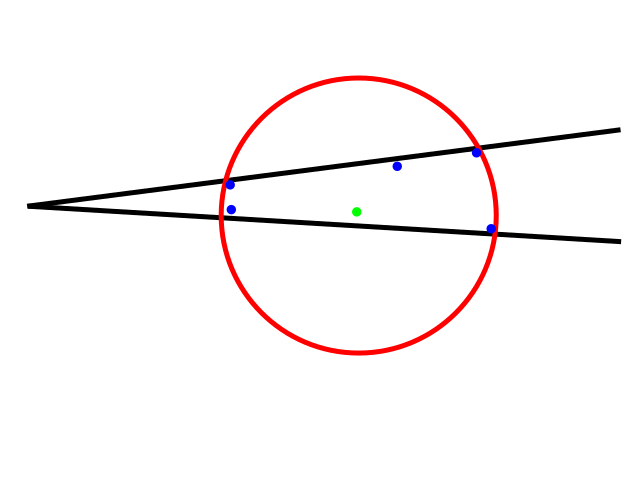
\includegraphics[scale=0.4]{images/bad_lambda.png}
    \caption{
    	\emph{Short:} An example of constraints limiting sample point choices.
    	\emph{Long:} If the constraints remove a large region of the trust region, there may be no feasible $\Lambda$-poised set.
    }
    \label{lspc}
\end{figure}

%As the number of dimensions grows the ratio of volume of the trust region intersect the feasible region to the feasible region can become smaller.

One way to handle this is to introduce a $\xi_{\text{cur}}$ which is allowed to decrease.
(Possibly, until a threshold is reached for maintaining a fixed $\Lambda$.)
If the new point does not improve the geometry of the set significantly, then there is no other point that would do better.
To test this, we introduce a constant $\delta_{\text{improv}}>0$ and require a new point to increase the current pivot by a factor greater than $\delta_{\text{improv}}$.
If the new point does not satisfy this test, we proceed with our current point and possibly decrease $\xi_{\text{cur}}$.
The new modified improvement algorithm is described in \cref{modified_model_improving_algorithm}:

\begin{algorithm}[H]
    \caption{Modified Model Improvement Algorithm}
    \label{modified_model_improving_algorithm}
    \begin{itemize}
        \item[\textbf{Step 0}] \textbf{(Initialization)} \\
            Initialize $i=1$.
            If the current sample set does not have $p$ points, repeat one of the current points. 
            Construct the Vandermonde matrix $V_{i,j} = \phi_j(\frac 1 {\Delta}(y^i - y^0))$.
            Initialize $0 < \ximin < \xi_{\text{desired}}$, $0 <\delta_{\text{improv}} < 1$,
            $  \xi_{\text{cur}} = \xi_{\text{desired}}$.
            
        \item[\textbf{Step 1}] \textbf{(Pivot)} \\
            Swap row $i$ with row $i_{\max} = \arg \max_{j|j\ge i} V_{j,i} $
        
        \item[\textbf{Step 2}] \textbf{(Check threshold)} \begin{itemize}
                \item[] If $|V_{i,i}| \ge \xi_{\text{cur}} $ then go to Step 3
                \item[] $ \hat y = \arg\max_{t \in \sampletrk \cap X} |\phi_i(t)|$
                \item[] If $\label{impossibly_poised} |\phi_i(\hat y)| < \ximin$ then \textbf{Stop}: the algorithm failed
                \item[] If $\xi_{\text{cur}} - |\phi_i(\hat y)| > \delta_{\text{improv}} \xi_{\text{cur}}$ then replace $V_{i,j}$ with $\phi_j(\hat y)$ and $\xi_{\text{cur}} \gets |\phi_i(\hat y)|$
            \end{itemize}
        
        \item[\textbf{Step 3}] \textbf{(LU)} \begin{itemize}
                \item[] Set $V_i \gets \frac{1}{V_{i,i}} V_i$
                \item[] Set $V_{,j} \gets V_{, j} - V_{i,j} V_{\bullet, i} \forall j=i \ldots p$
            \end{itemize}
            $i \gets i+1$
            Go to step 1 unless $i > p$
    \end{itemize}
\end{algorithm}

The \emph{ConstructTrustRegion} subroutine for this approach follows the prototype with $\sampletrk = \searchtrk = \feasible \cap \outertrk $.
As is usual, we may also wish to remove points larger than a certain radius from the current model center.
% If a lower bound $\kappa_{\phi}$ on the maximum value of each polynomial is known ahead of time, then the check on \cref{impossibly_poised} is not needed.
% That is, for a given set of linear constraints and largest trust region radius, it may be possible to calculate $\xi_{\text{min}} \le \kappa_{\phi} \le \max_{V}\max_{j}\max_{i}\|\phi_i(y^j)\|$.

%Another interesting approach we have not investigated is to decrease the size of the sample set when a new point cannot be computed.

%The analysis for this approach may be more difficult.




\section{Ellipsoidal Trust Region Approach}

If we adopt the ellipsoidal trust region approach to maintain a feasible inner trust region with a ``nice" shape we ensure of a stronger version of \cref{accuracy}.
Namely, we know from \cref{ellipsoidal_lambda} that 
\begin{align*}
    \|\mfk(x) - \nabla f(x) \| \le \kappa_g \Delta_{k} \quad \forall x \in \searchtrk.
\end{align*}
If we also choose our trial point with \cref{search_a_little}, we have no guarantee of satisfying the efficiency condition \cref{efficiency} because $\dk$ is the outer trust region radius.
However, the model will likely be more accurate over this region.

%If bounds can be shown relating the model error of the inner trust region to the outer trust region, then we will satisfy \cref{accuracy}.
%In this case, classical methods ensure that $\|\nabla f(x^{(k)}) - \nabla m_f(x^{(k)})\| < \Delta_{inner} \le \dk$.

\subsection{Circular Trust Region}
The simplest approach to maintaining a feasible trust region is to set the inner trust region radius sufficiently small.
Within the \emph{ConstructTrustRegion} subroutine, this method sets the trust region radius to the distance to the closest constraint:
$\outertrk = B_2\left(\xk, \min\left\{\dk, \min_{i}\frac{\left|A_i\xk - b_i\right|}{\left\|A_i\right\|} \right\}\right)$.
In practice, this does not work well as the radius can become too small to allow adequate progress.

Two general strategies were considered for addressing this issue as illustrated in \cref{options_basis}.
One option is to shift the center of the inner trust region as long as it remains within the outer trust region.
The second option is to elongate the trust region along the nearest constraint as discussed in the next section.
Of course, both of these can be done at the same time.


\begin{figure}[ht]
    \centering
    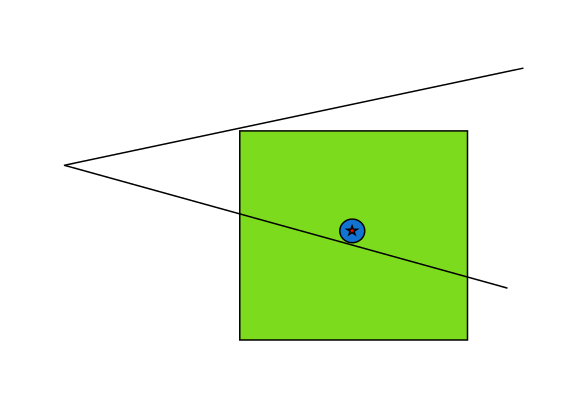
\includegraphics[width=200px]{images/small_circle.png}
    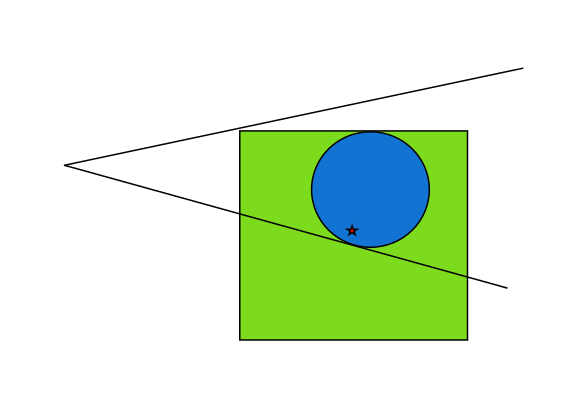
\includegraphics[width=200px]{images/shifted_center.png}
    \caption{
    	\emph{Short:} The advantage of not requiring the sample region center to be the trust region center.
    	\emph{Long:} When the current iterate is too close to a constraint, the circular trust region becomes too small.
    	Shifting the trust region center helps remedy this.
    	The star is the current iterate, the green is the outer trust region, and blue the inner.
    }
    \label{options_basis}
\end{figure}

\subsection{Ellipsoid Choices}

In order to address this issue we considered using ellipsoidal trust regions.
Whereas the circle does not allow improvement when the current iterate lies along a constraint, an ellipsoid elongates along this constraint.
In figure \cref{ellipse_adv}, we have this type of iterate, but by using an ellipsoid we are still able to search towards the vertex of the feasible region.
\begin{figure}[ht]
    \centering
    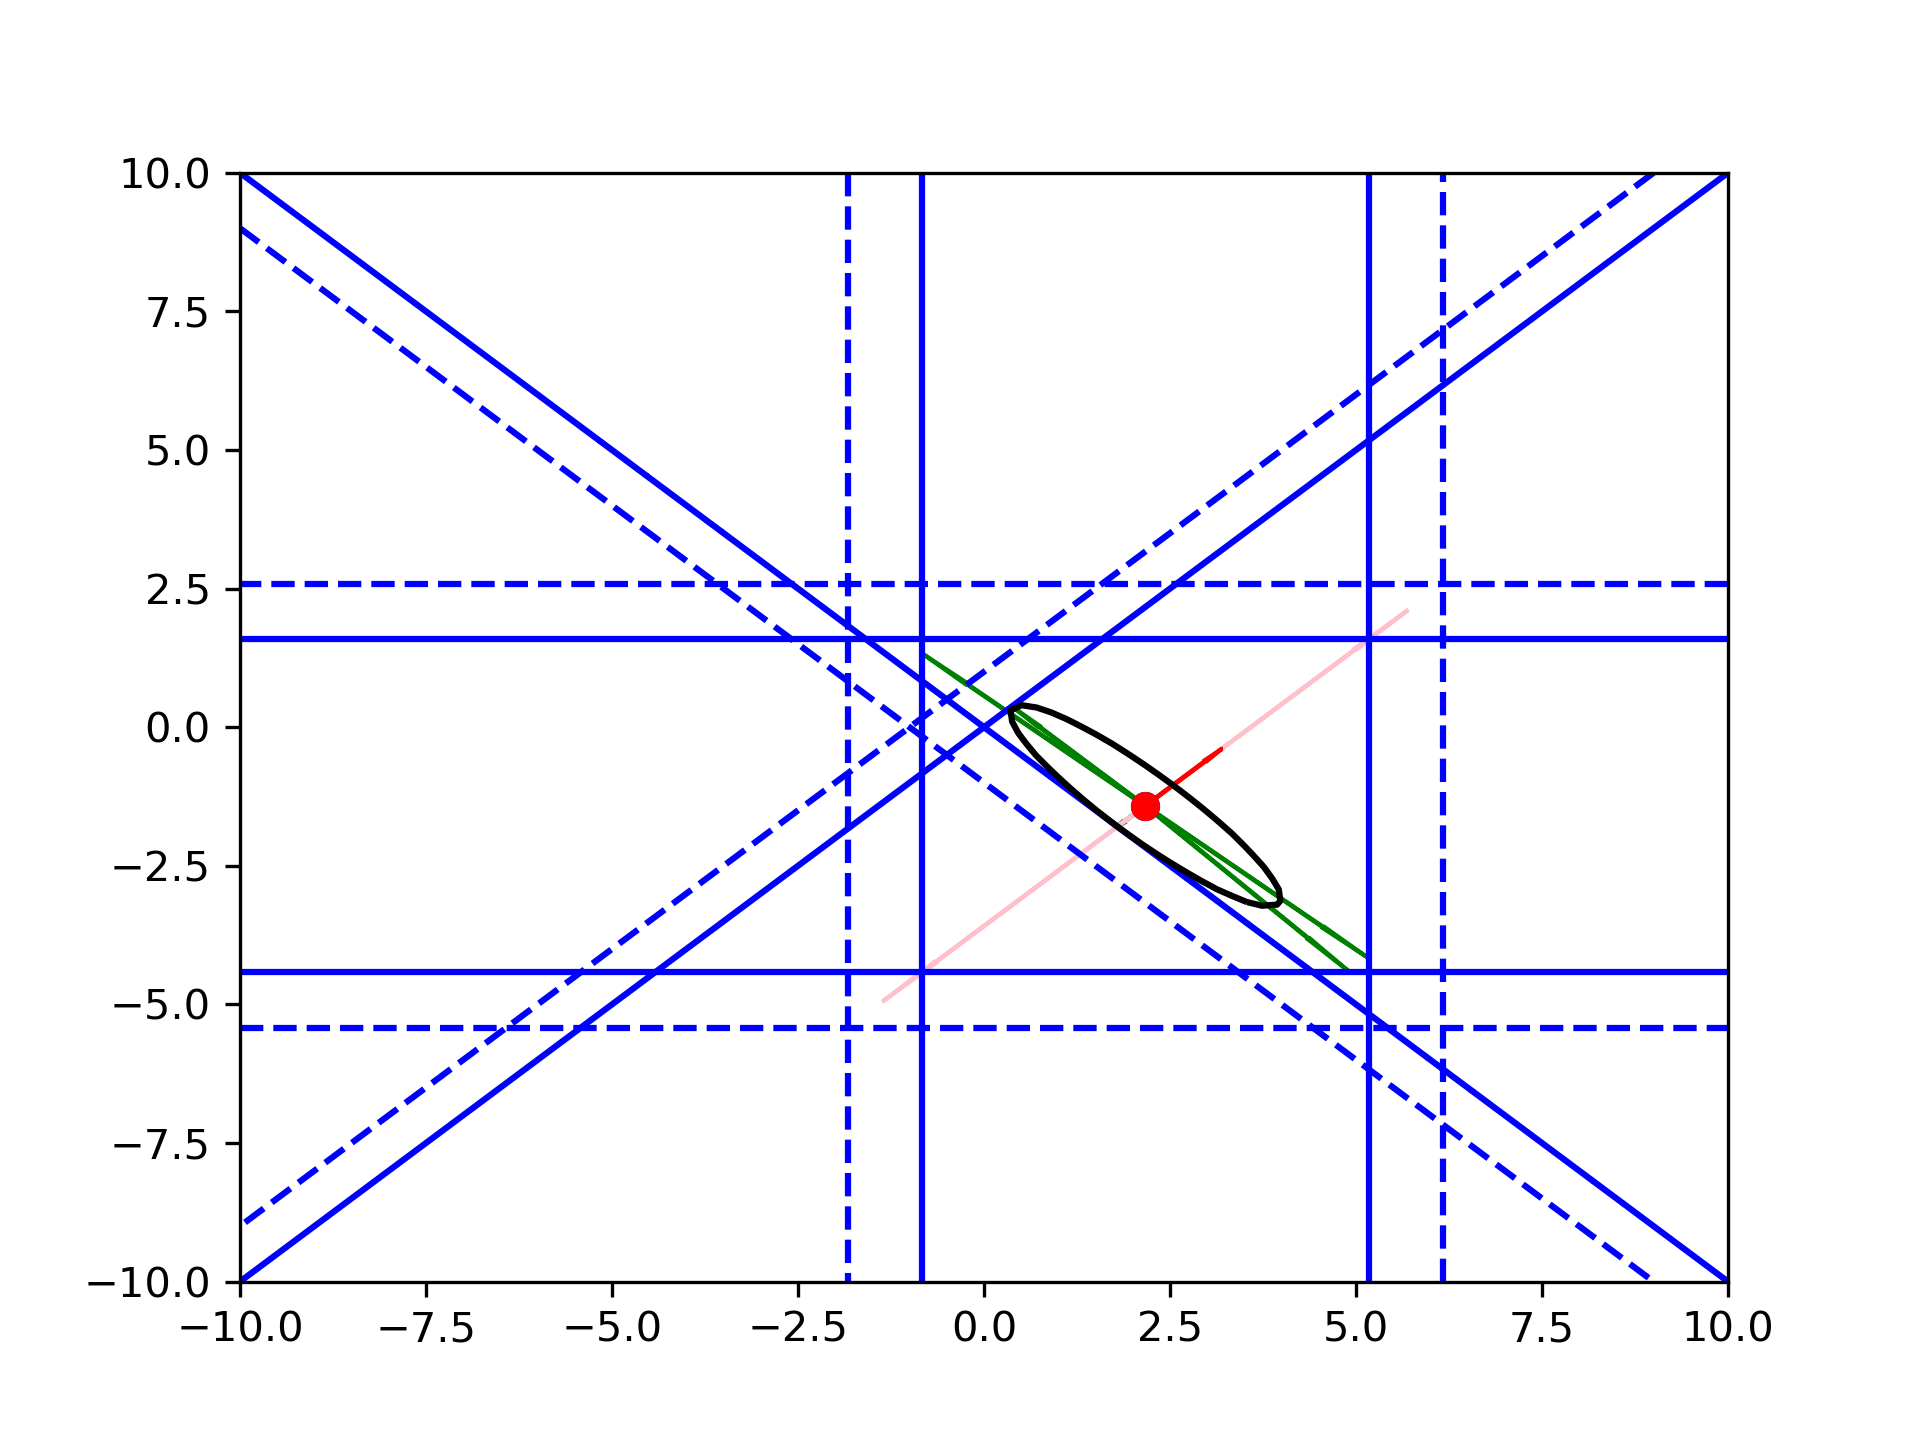
\includegraphics[scale=0.4]{images/advantage_of_ellipse_2.png}
    \caption{
    	\emph{Short:} An ellipsoidal trust region allows for more progress than a circular trust region.
    	\emph{Long:} Although the center of the ellipsoid is close to the boundary of the constraints, it can elongate to allow progress.
    }
    \label{ellipse_adv}
\end{figure}


More specifically, at iteration $k$, we choose a scaling factor $\sdk$ and solve for an ellipsoid center $\ck \in \Rn$ and positive definite matrix $\qk$ to define an ellipsoid
\begin{align*}
\ellipsek = \left\{x \in \Rn \bigg| \; \frac 1 2 \left(x - \ck\right)^T\qk\left(x - \ck\right) \le \sdk \right\}.
\end{align*}
The simplest approach is to simply let the center of the ellipsoid be the current iterate: $\ck = \xk$.


\subsection{Maximal Volume Ellipsoid}

\label{ellipse_optimization}

Here, we first solve the problem of finding the maximum-volume ellipsoid given the center.
Later we perform a search over different centers of the ellipsoid.
%Because of this, we will first show how to find an ellipsoid with maximum volume given a fixed center.
We adopt a method similar to that described in \cite{Khachiyan1993}.
For now, we also let $\sdk = 1$.

Given a polyhedron $P$ defined by an $m \times n$ matrix $A$, $P = \{ x \in \Rn\; | \;  Ax \le b \}$.
we wish to find the maximum-volume ellipsoid $E \subset P$ centered at a point $\mu \in P$.

Let $\bar{b} = b - A\mu$ and $d = x - \mu$ so that the polyhedron becomes
\begin{align*}
P = \{ \mu + d \in \Rn \; | \;  Ad \le \bar{b} \}
\end{align*}
Then, the ellipsoid can then be centered at zero, and defined by a symmetric positive definite matrix $Q \succ 0$:
\begin{align*}
E = \{ d \in \Rn \; | \; \frac 1 2 d^T Q d \le 1 \}.
\end{align*}
Our goal is to determine $Q$ to maximize the volume of $E$ such that $\mu + E \subset P$.
Define the auxiliary function $f(d) = \frac 1 2 d^T Q d$ so that $E = \{ d \in \Rn\; | \; f(d) \le 1 \}$.

Because $Q$ is positive definite, $f$ has a unique minimum on each hyper-plane $A_i d = b_i$.
Let this minimum be $d^{(i)} = \argmin_{A_id =\bar{b}_i} f(d)$ for $i=1,\ldots,m$.
By the first order optimality conditions, there exists a $\lambda \in \Rm$ such that
\begin{align*}
\nabla f(d^{(i)}) = Q d^{(i)} = \lambda_i A_i 
\Longrightarrow d^{(i)} = \lambda_i Q^{-1}A_i \quad \forall 1\le i\le m
\end{align*}
We also know that
\begin{align*}
A_i^T d^{(i)} = \bar{b_i} \Longrightarrow
A_i^T \lambda_i Q^{-1}A_i = \bar{b_i} \Longrightarrow
\lambda_i = \frac {\bar{b_i}}{A_i^T  Q^{-1}A_i}
\end{align*}
so that
\begin{align*}
d^{(i)} = \lambda_i Q^{-1}A_i = \frac {\bar{b_i}}{A_i^T  Q^{-1}A_i}  Q^{-1}A_i \quad \forall 1\le i\le m.
\end{align*}

Because $E \subset P$, we also know that $f(d^{(i)}) \ge 1$ for each $i$. Thus,
\begin{align*}
\frac 1 2 (d^{(i)})^{T} Q d^{(i)} \ge 1 \\
\Longrightarrow \frac 1 2 \bigg(\frac {\bar{b}_i}{A_i^T  Q^{-1}A_i}  Q^{-1}A_i\bigg)^{T} Q \frac {\bar{b}_i}{A_i^T  Q^{-1}A_i}  Q^{-1}A_i \ge 1 \\
\Longrightarrow \frac 1 2 \frac {1}{A_i^T  Q^{-1}A_i}  \bar{b_i} A_i^T Q^{-1} Q \frac {\bar{b_i}}{A_i^T  Q^{-1}A_i}  Q^{-1}A_i \ge 1 \\
\Longrightarrow \frac 1 2 \frac {1}{A_i^T  Q^{-1}A_i}  \frac {\bar{b_i}^2}{A_i^T  Q^{-1}A_i}  A_i^T Q^{-1}A_i \ge 1 \\
\Longrightarrow \frac 1 2  \frac {\bar{b_i}^2}{A_i^T  Q^{-1}A_i} \ge 1 \\
\Longrightarrow \frac 1 2 \bar{b_i}^2\ge A_i^T  Q^{-1}A_i \\
\Longrightarrow A_i^T  Q^{-1}A_i \le \frac 1 2 \bar{b_i}^2
\end{align*}

Because the volume of the ellipsoid is proportional to the determinant of $Q^{-1}$, the maximal ellipsoid is defined by

\begin{align}
 Q = V(\mu) = \sup_{Q \succeq 0} \det(Q^{-1})  \label{ellipse_1} \\
s.t. \quad A_i^T Q^{-1} A_i \le \frac 1 2 \bar{b_i}^2
\end{align}


\subsubsection{Poisedness over Ellipsoidal Trust Regions}
\label{ellipsoidal_lambda}

% TODO: Find a better reference
It is possible to show $\Lambda$-poisedness for an ellipsoidal region with a change of variables to the ball centered around the origin.
We wish to construct a model for $f(x)$ in the ellipsoidal region
$\ellipsek = \{x \in \Rn | (x - \ck)^T\qk(x - \ck) \le 1\}$ for some symmetric, positive definite
$\qk \in \mathbb R^{n\times n}$ and some center $\ck \in \Rn$.
We can give $\qk$ its eigen-decomposition $\qk = L D^2 L^T$, where $L^TL = I$ and $D$ is a diagonal matrix with nonnegative entries.
If we let $\delta = \max_{x\in \ellipsek}\|x-\ck\|$, then the transformation $T(x) = \delta DL^T(x - \ck)$ maps $ \ellipsek $ to the $\delta$ ball $\{u = T(x) \in \Rn \; | \; \|u\| \le \delta\}$.
Conversely, $ T^{-1}(u) = \frac 1 {\delta} LD^{-1}u + \ck$ maps the $\delta$ ball to the ellipsoidal region $ \ellipsek $.

% \cref{fully_quadratic}

\begin{theorem}
\label{shifted_ellipsoid}
Let a positive-definite, symmetric $n\times n$ matrix $\qk$, a vector $\ck \in \Rn$, and constant $\sdk > 0$ be given.
Let $\qk = L D^2 L^T$ be the eigen-decomposition of $\qk$ where $L^TL = I$ and $D$ is a diagonal matrix with positive entries.
Also, let $\delta = \max_{x\in \ellipsek}\|x-\ck\|$, 
and define the transformation $T(x) = \delta DL^T(x - \ck)$.
Let $\hat m_f(u)$ be a model of the shifted objective $\hat f(u) = f(T^{-1}(u))$ in the $\delta$ ball such that
there exist constants $\kappa_{ef}, \kappa_{eg}, \kappa_{eh} > 0$ such that for all $\left\{u \in R^n | \;\|u\| \le \delta \right\}$, we have
% for all $u \in B(0 ; \delta)$ we have the following error bounds:
\begin{align*}
\left|\hat m_f(u) - \hat f(u)\right| \le \kappa_{ef} \delta^3\\
\left\|\nabla \hat m_f(u) - \nabla \hat f(u)\right\| \le \kappa_{eg}\delta^2\\
\left\|\nabla^2 \hat m_f(u) - \nabla^2 \hat f(u)\right\| \le \kappa_{eh}\delta.
\end{align*}

Then, with
\begin{align*}
\kappa_{ef}' = \kappa_{ef} \\
\kappa_{eg}' = \kappa_{eg}\sqrt{\condition(\qk)} \\
\kappa_{eh}' = \kappa_{eh}\condition(\qk),
\end{align*}
we have that for all $x \in \ellipsek$,
the model function $m_f(x) = \hat m_f(T(x))$ will satisfy
\begin{align*}
\left| m(x) - f(x)\right| \le \kappa_{ef}'\delta^3 \\
\left\|\nabla  m(x) - \nabla  f(x)\right\| \le \kappa_{eg}'\delta^2 \\
\left\|\nabla^2 m(x) - \nabla^2 f(x)\right\| \le \kappa_{eh}'\delta.
\end{align*}
\end{theorem}

\begin{proof}

% Notice  that for all $x\in \ellipsek$ we have 
% \begin{align*}
% \|x-c\| \le \delta \\
% \|T(x-c)\| \le \delta \\
% \end{align*}
% so that $\frac{\|T(x-c)\|}{\|x-c\|} \le 

We know that $\delta = \frac 1 {\sqrt{\lambda_{\text{min}}(\qk)}} = \frac 1 {\min_{i} D_{i, i}}$.
This means,
\begin{align*}
\kappa(\qk) = \kappa(D^2) = \frac{\max_{i}D_{i,i}^2}{\min_{i}D_{i,i}^2} = \delta^2 \max_{i}D_{i,i}^2 = \delta^2 \|D\|^2 \\
\|D\| = \frac 1 {\delta} \sqrt{\kappa(\qk)} \le \frac{\kappa_{\lambda}}{\delta}.
\end{align*}

Also, $\delta \le \dk$ as the ellipse is constructed within the outer trust region.

Then, we have for all $\left\{u = T(x) \; | \; \|u\| \le \delta \right\} \Leftrightarrow x \in \ellipsek$

\begin{align*}
\left| m_f(x) - f(x)\right| = \left|\hat m(u) - \hat f(u)\right| \le \kappa_{ef}'\dk^3.
\end{align*}

Similarily, for the gradient we find:

\begin{align*}
\| \nabla m_f(x) - \nabla f(x)\| = \delta\left\|DL^T\left(\nabla\hat m_f(u) - \nabla \hat f(u)\right)\right\| \\
\le \delta \|DL^T\|\|\nabla \hat m_f(u) - \nabla \hat f(u)\| 
\le \sqrt{\kappa(\qk)}\kappa_{eg} \delta^2
\end{align*}

Finally, we show that for the Hessian:

\begin{align*}
\left\| \nabla^2 m_f(x) - \nabla^2 f(x)\right\| = \delta^2\left\|DL^T\left(\nabla\hat m_f(u) - \nabla \hat f(u)\right)LD^T\right\| \\
\le \delta^2 \left\|D\right\|^2\left\|\nabla \hat m_f(u) - \nabla \hat f(u)\right\| \le \kappa\left(\qk\right)\kappa_{eh} \delta
\end{align*}

\end{proof}

This shows that in order to have strongly quadratic model functions, we need only bound the condition number of $\qk$.
For the purposes of a convergence proof, we need only satisfy the weaker accuracy condition \cref{accuracy}.
Notice that in practice the model functions do not need to be mapped to the $\delta$ ball, because $\Lambda$-poisedness is scale invariant \cite{introduction_book}.
The implications of this proof are discussed futher in the convergence discussion \cref{linear_convergence_discussion}.


\subsubsection{Ellipsoid Choices}

There are a number of issues to be solved to define this ellipsoid:
\begin{itemize}
\item How do we ensure that $\xk \in \ellipsek $?
\item How do we choose $\ellipsek$ in such a way that it does not limit travel along a decent direction?
\item How do we choose the center of the ellipsoid $\ck$?
\end{itemize}

% \item How do we choose $\ellipsek$ to make the  ellipsoid as large as possible while ensuring that $ \ellipsek \subset \outertrk \cap \feasible $?

If $\xk \not \in \searchtrk $, the ellipse may not even contain a point with any reduction.
Thus, we have implemented a few ways of ensuring the current iterate is within the search trust region.
This can be done by either of the following two options:
\begin{itemize}
\item Adding a constraint to the ellipsoid problem to include the original point.
\item Expand the size of the ellipsoid.
\end{itemize}

%IMAGES GO HERE

\paragraph{Adding a constraint.}
In order to include the original point as a constraint, we add a constraint to the definition of the ellipsoid of the following form:
\begin{align*}
\frac 1 2 \left(\xk - \ck\right)^T\qk\left(\xk - \ck\right) \le \sdk.
\end{align*}
Constraints of this nature make finding the ellipsoid much more expensive:
the optimization problem we construct uses ${\qk}^{-1}$ as decision variables, so that constraints in terms of $\qk$ must model matrix inversion.

\paragraph{Increase the size.}
An alternative is to scale $\qk$ by a constant.
We use the scaling factor $\sdk$ defined by
\begin{align*}
\sdk = \max \left\{1, \frac 1 {2} \left(\xk - \sdk\right)^T \qk \left(\xk - \sdk\right)^T \right\}
\end{align*}
and let the ellipsoid be:
\begin{align*}
\ellipsek = \left\{x \in \Rn \bigg| \left(x - \ck\right)^T \qk \left(x - \ck\right) \le 2\sdk\right\}
\end{align*}
However, this means that in general $\ellipsek \not \subset \feasible$ so that the trust region subproblem must contain constraints for both the ellipsoid and the feasible region: 
$\searchtrk = \ellipsek \cap \feasiblek$.

To help mitigate the second issue, we maximize the volume of the ellipsoid.
However, the choice of ellipsoid center can still limit travel along a decent direction.
Choosing the best center is the topic of the next section.\


\subsection{Searches for the Center}

We consider several different approaches for determining the trust region center $\sdk$.
In this case, our \emph{ConstructTrustRegion} subroutine searches over multiple centers of the ellipsoid, however it may not need to construct the model functions for each until it has found a desirable ellipsoid.


\subsubsection{Outer Trust Region Search}

One approach is to search all possible centers within $ \feasible \cap \outertrk $.
That is, we solve:
\begin{align*}
\sdk = \sup_{c \in \feasible \cap \outertrk} V(c)
\end{align*}
where $V(c)$ is the volume of the ellipsoid defined in \cref{ellipse_1}.
%The search within the \emph{ConstructTrustRegion} is allowed to go anywhere within $ \feasible \cap \outertrk$.
This has the advantage that it captures much of the feasible region.
However, one problem with this search is that it can force the trust region away from the desired direction.
Notice that in \cref{ellipse_runs_away}, although the ellipsoid found has larger volume than before being shifted, this ellipsoid contains points farther from the corner containing the minimizer.

\begin{figure}[ht]
    \centering
    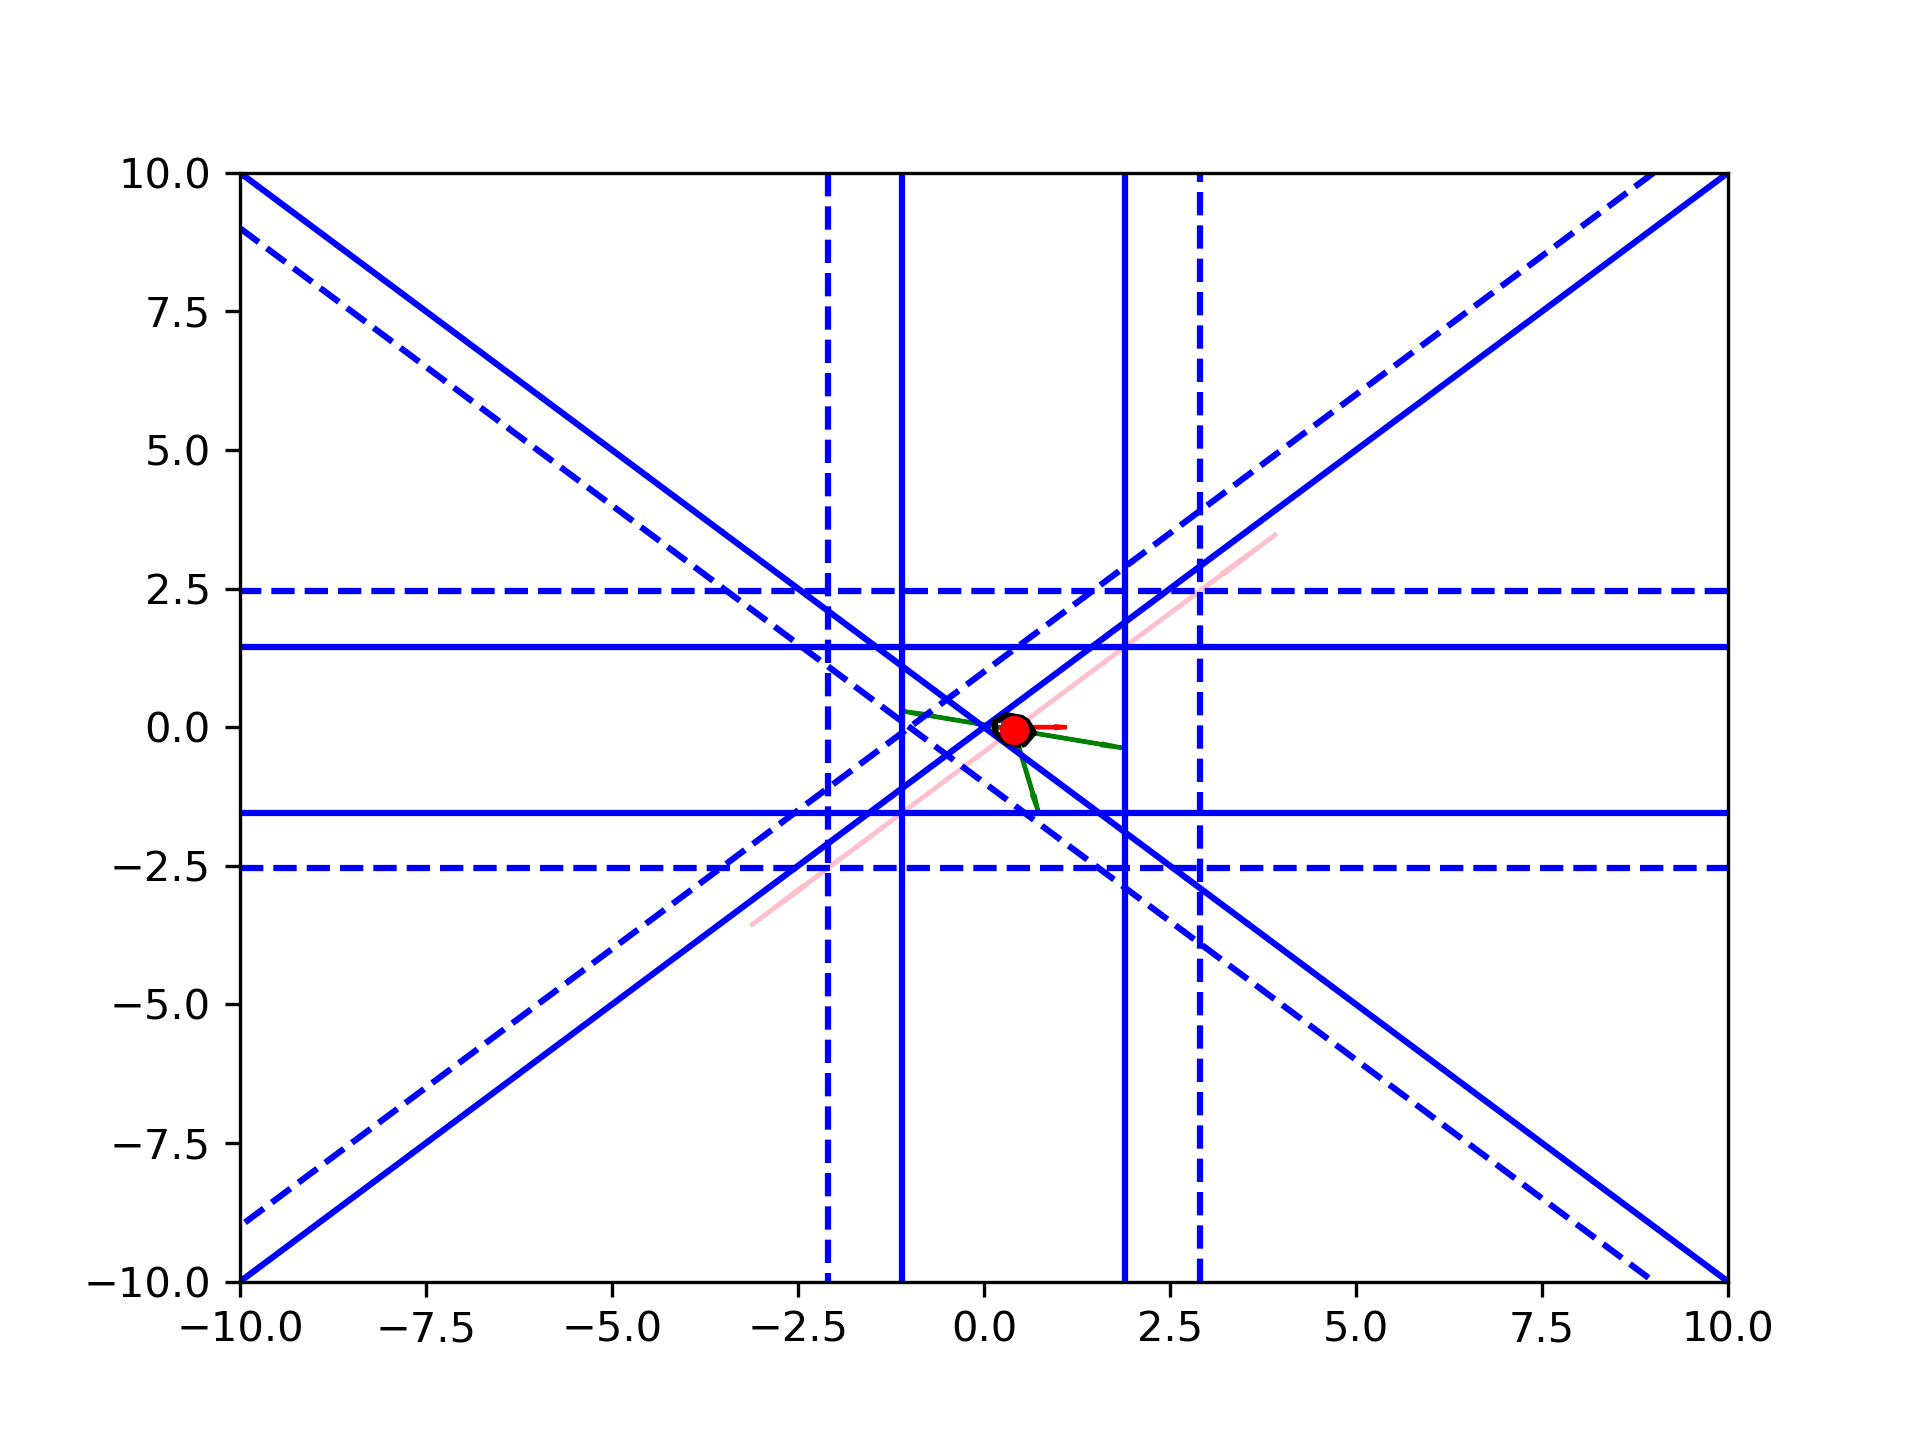
\includegraphics[scale=0.4]{images/everything_runs_1.png}
    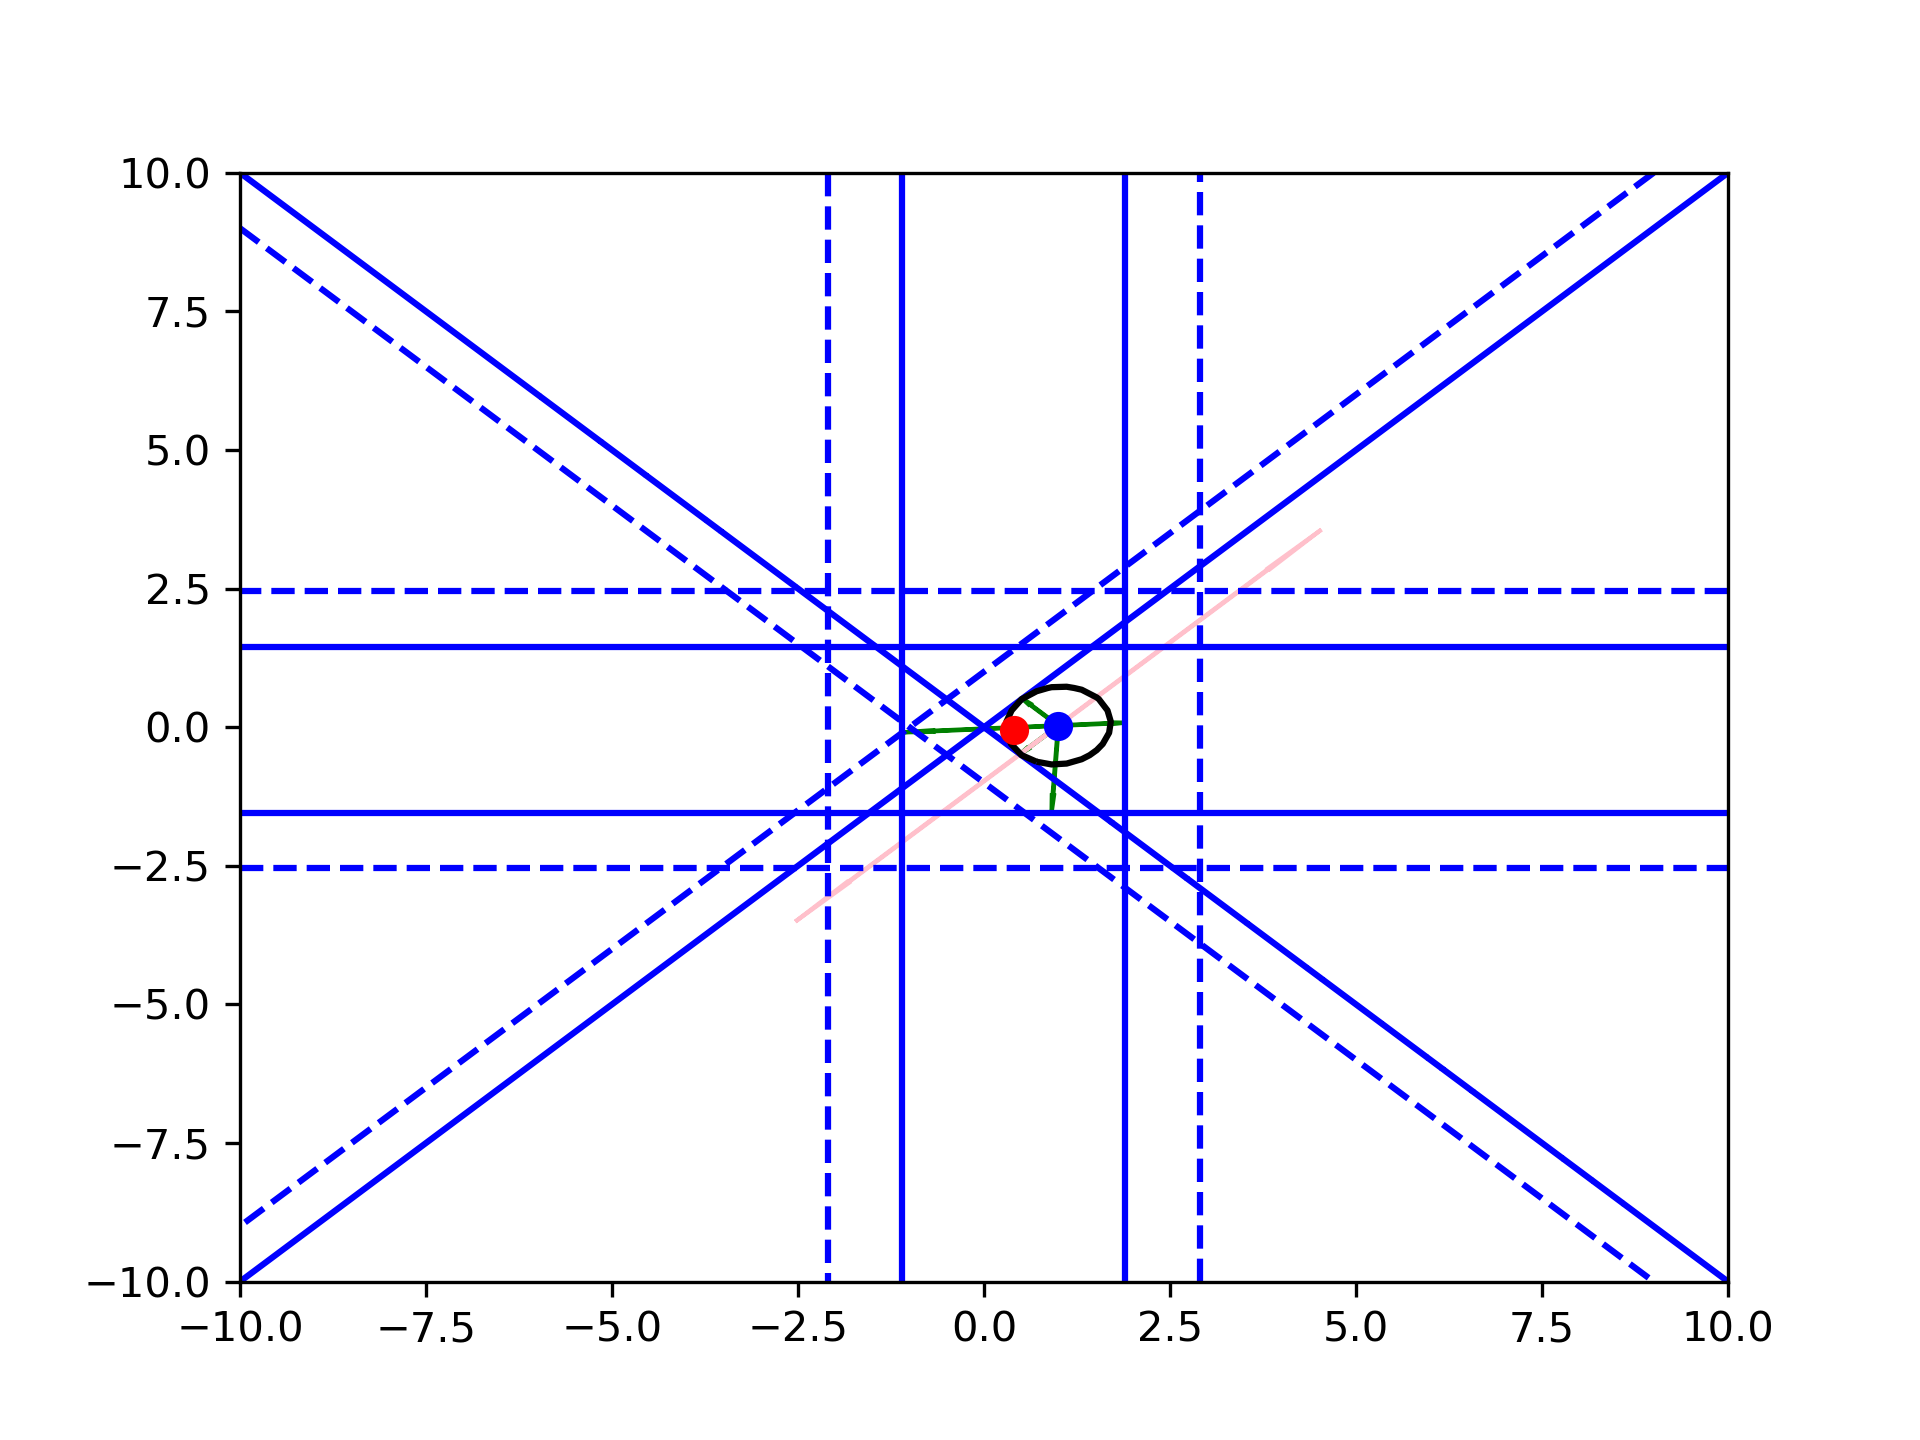
\includegraphics[scale=0.4]{images/everything_runs_2.png}
    \caption{
    	\emph{Short:} An example of how the search for the sample region center can go wrong.
    	\emph{Long:} On the left, a very small sample region is selected; however its proximity to the the minimizer over the outer trust region makes the model more accurate at the minimizer.
    	On the right, a sample region with larger volume is chosen, but it is further from the trust region minimizer.
	}
    \label{ellipse_runs_away}
\end{figure}


One attempt to fix this problem is by limiting the search direction for the center of the ellipsoid.


\subsubsection{Line Searches}
Although $\mfk$'s minimizer over $\outertrk$  can appear anywhere, there are some reasons for expecting it to be at a ``vertex."
If it lies in the interior, there is little need for using constrained approaches once near the solution.

%The ellipsoid with maximum volume, however, tends to lead $ \sampletrk $ away from vertices.
One way of trying to ensure a feasible direction towards a vertex, while still allowing a larger volume ellipsoid, is by limiting the search for the new center to lie on line segments starting at the current iterate $\xk$.

For example, our first attempt was to simply search a line directed orthogonally away from the closest constraint.
This has obvious problems as shown in \cref{first_line_search}: we should avoid letting the new center get closer to another constraint.

\begin{figure}[ht]
    \centering
    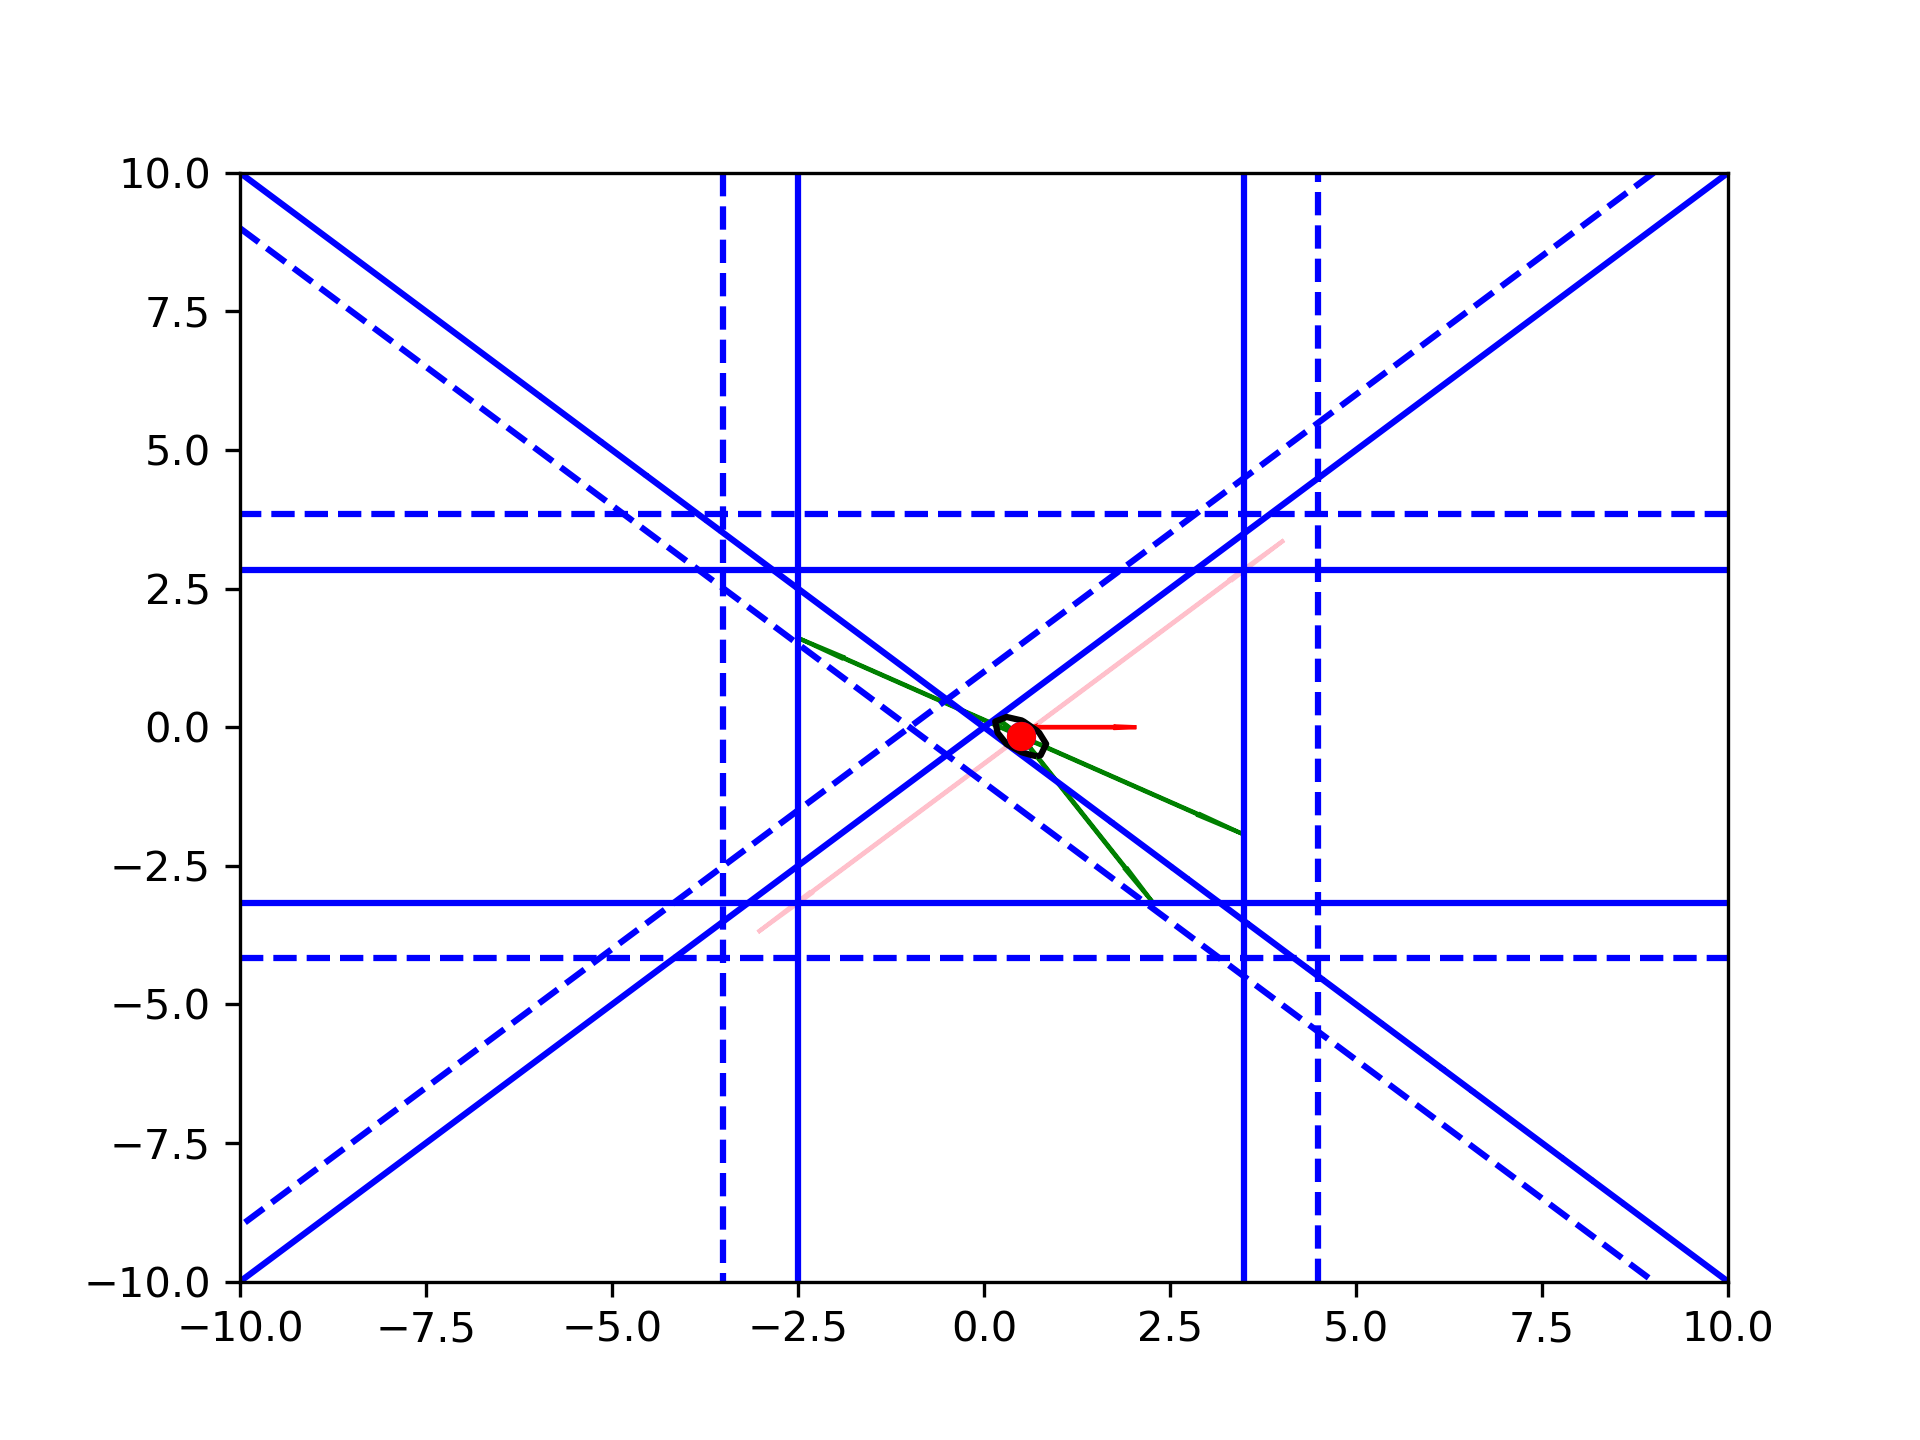
\includegraphics[scale=0.4]{images/line_1.png}
    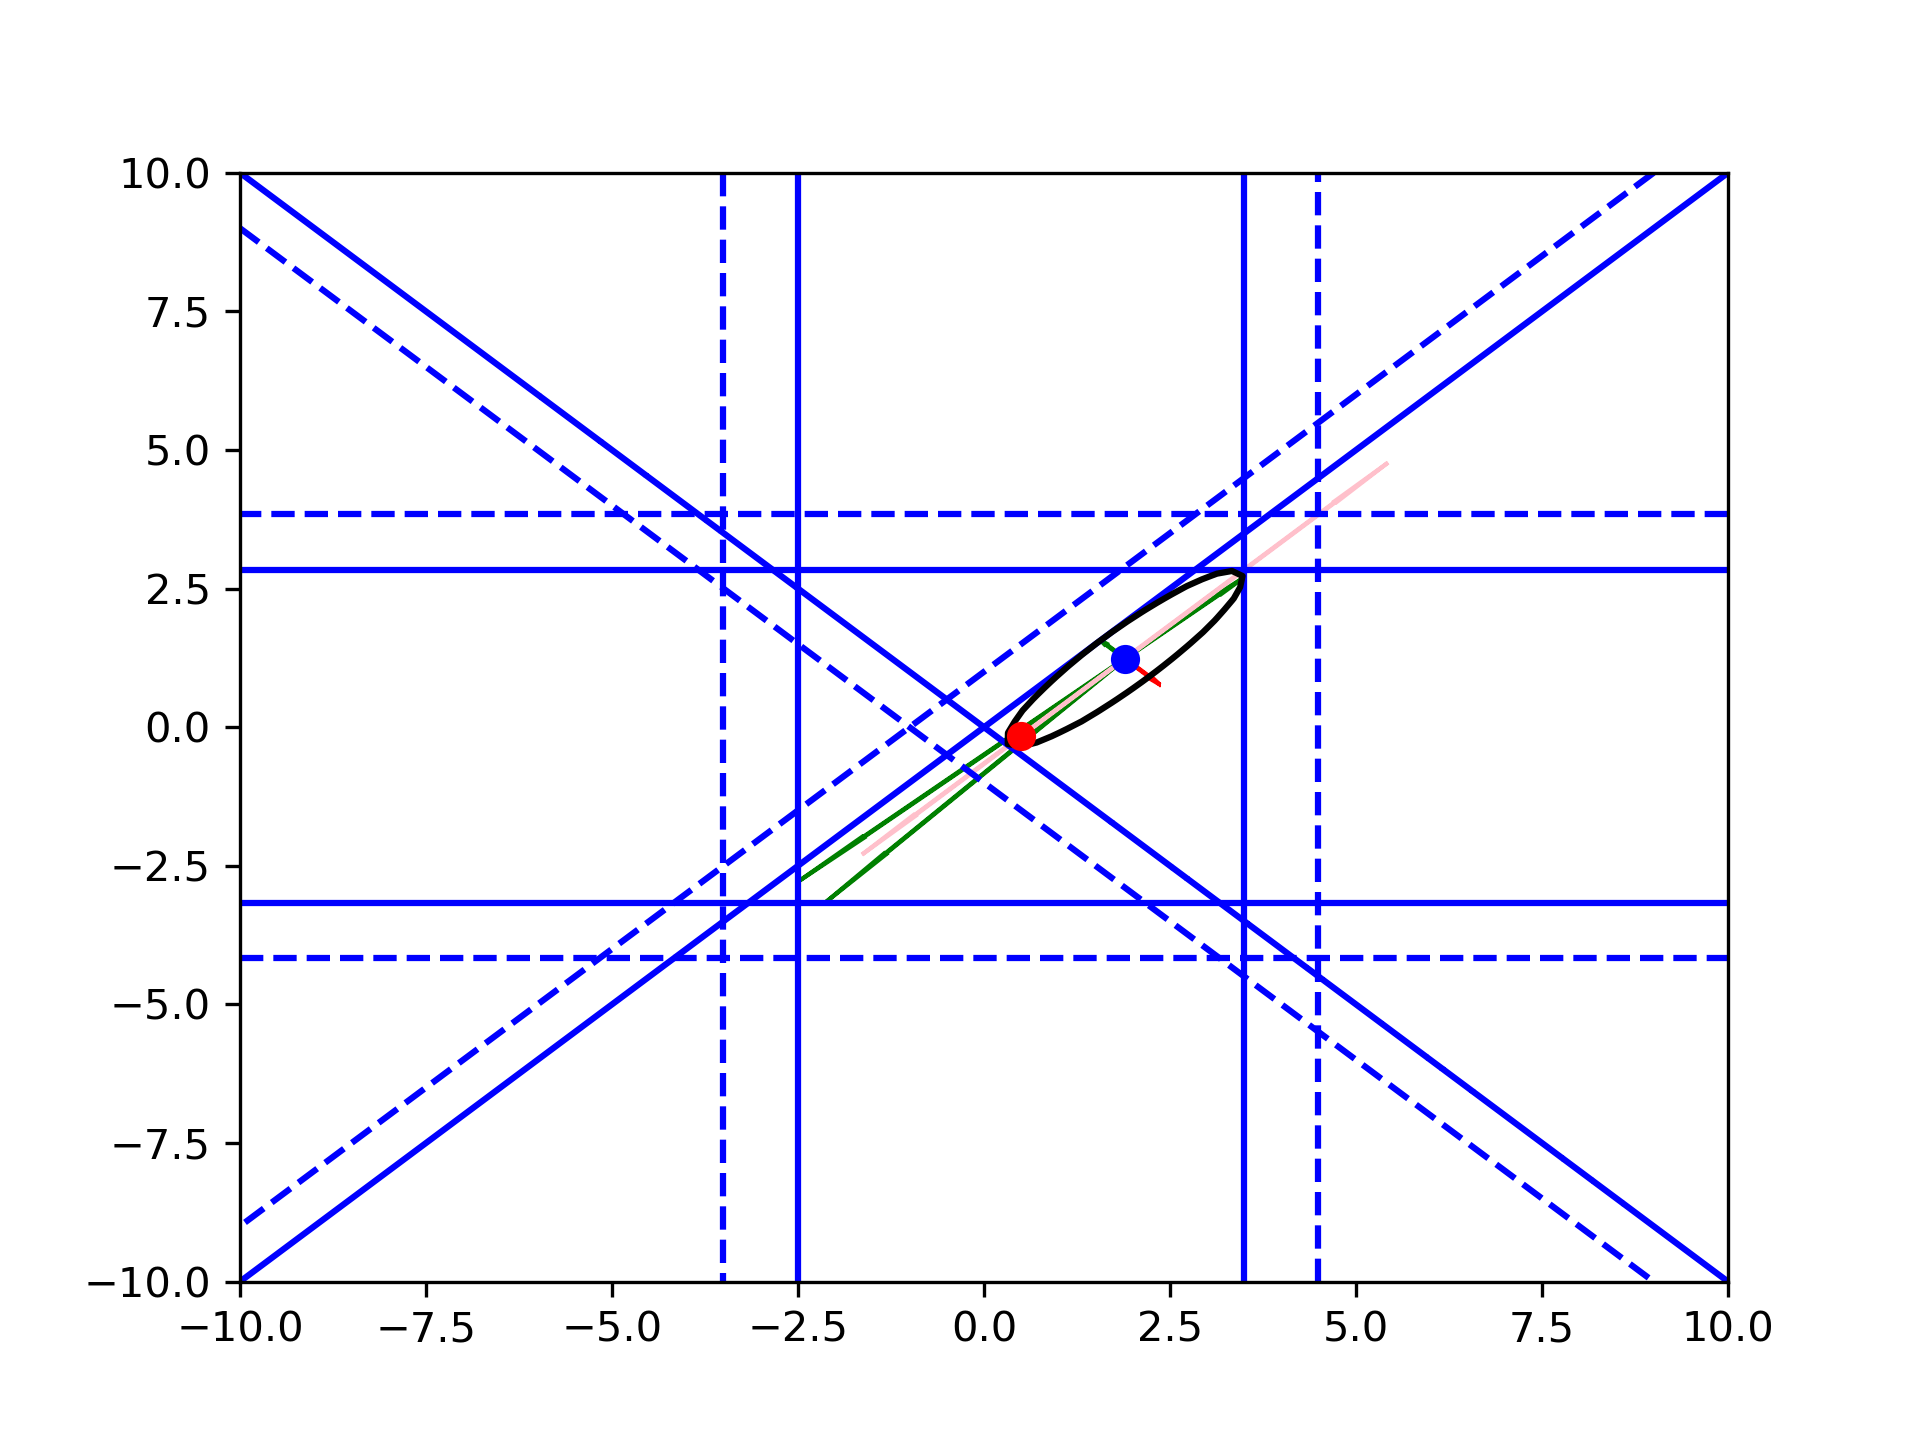
\includegraphics[scale=0.4]{images/line_2.png}
    \caption{
    	\emph{Short:} Why only considering the nearest constraint is not sufficient. 
    	\emph{Long:} On the left is the starting ellipsoid.
    	By choosing centers further away from only the nearest constraint, the ellipsoid becomes narrow as another constraint is limiting the length of the second axis.
	}
    \label{first_line_search}
\end{figure}

To fix this, we break the search space within the \emph{ConstructrustRegion} subroutine into segments based on the nearest constraints.
% For a given distance $d$, let the indices $i$ for which $\frac {|A_i x - b|}{\|A_i\|} \le d$.
The algorithm works by choosing a set of up to $n_{\text{points}}$ points $s_1, s_2, \ldots, s_{n_{\text{points}}}$ that are each equidistant to a subset of the constraint's faces.
The center search then considers points along the line segments between these points.
% Namely, it starts at the current iterate and travels along a ray away from all the closest constraints until it reaches a point equidistant to yet another constraint.

More precisely, the first point is chosen to be the current iterate: $s_1 = \xk$.
The algorithm then repeats the following process for $i$ from $1$ to $n_{\text{points}}$.
First, compute the set of nearest constraints, where the distance from a point $x$ to a constraint $A_i$ is given by $d(A_i, x) = \frac {|A_i x - b|}{\|A_i\|}$.
While finding the next point $s_{i+1}$, let  $A_E$ be a normalized array of the equidistant faces $\{\frac{A_i}{\|A_i\|} | d(A_i, s_i) = \min_j d(A_j, s_i), i = 1, 2, \ldots, m\}$ and $b_E$ be the rows' corresponding values of $b$.
All other faces are called the remaining faces, and construct the matrix $A_R$ and vector $b_R$.
It then finds a search direction $p  = r{A_E}^T$ as a linear combination of the normal vectors to the equidistant faces.
%When the constraint violation of $s_i$ is non-zero, this search ray can be found by finding the point that doubles the current slack ${A_E}s_i-{b_E}$.
%This is given by $r{A_E}^T$ where $r$ solves the linear system ${A_E}(s_i + r{A_E}^T) - b_E = 2 ({A_E}n_i - b_E)$.
%If the current violation is zero, then the right hand side can be set to a vector of all ones to ensure that all slacks violations are the same: $A_E(s_i + r{A_E}^T) - b_E = 1$.
This search ray can be found by setting the slack to each equidistant face to a vector of all ones: $A_E(s_i + r{A_E}^T) - b_E = 1$.
We can travel along this ray until we reach a point that is the same distance to a remaining face.
Specifically, we can travel by 
\begin{align}
t = \argmin_j {\frac{d({A_E}_0, s_i) - d({A_R}_j, s_i)}{ {A_R}_j - d({A_E}_0) p} | ({A_R}_j - d({A_E}_0) p > 0 }. 
\end{align}

We can then set $s_{i+1} = s_{i} + t p$.

Of course, $n_{\text{points}}$ must be less than or equal to $n + 1$ in order for this to be defined.
Also, the algorithm must stop early if $A_E$ contains parallel faces.

% if we let $\nabla \modelconstrainti\left(\xk\right) = A_i$ be the $i$th row of $A$, then we define the distance from a search point $s$ so the $i$th constraint to be


This means that we can define a class of searches that each limit the number of line segments to search $n_{\text{points}}$.

In figure \cref{line_can_run}, the red line shows the line segments equidistant their closest constraints.
Notice that with two line segments, the algorithm can already choose new centers further from the vertex.

% TODO: REPLACE PICTURES
\begin{figure}[ht]
    \centering
    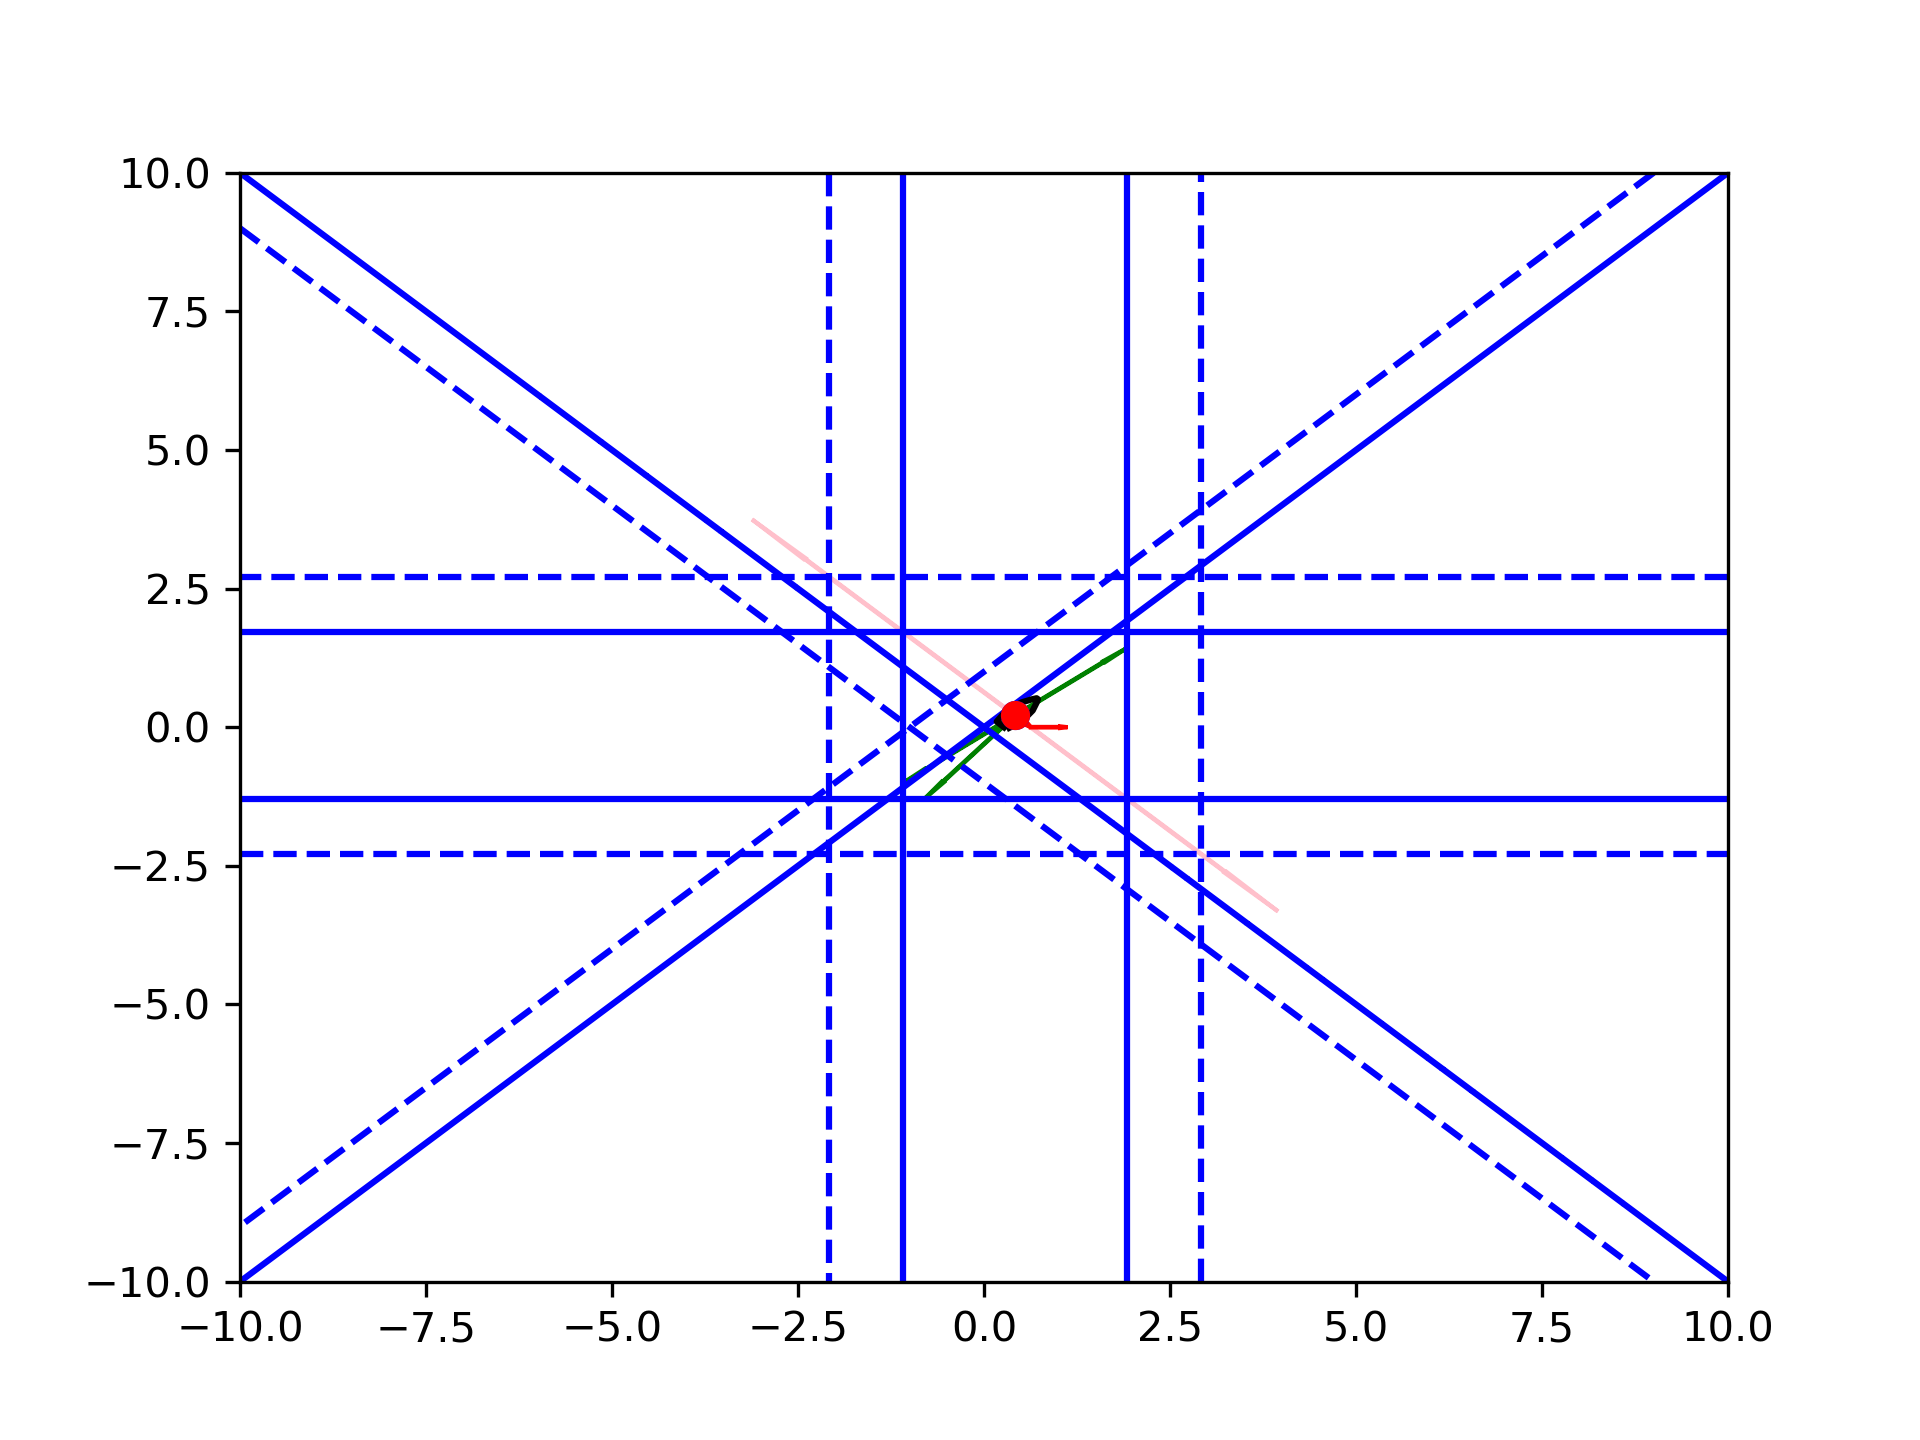
\includegraphics[scale=0.4]{images/run_away_1.png}
    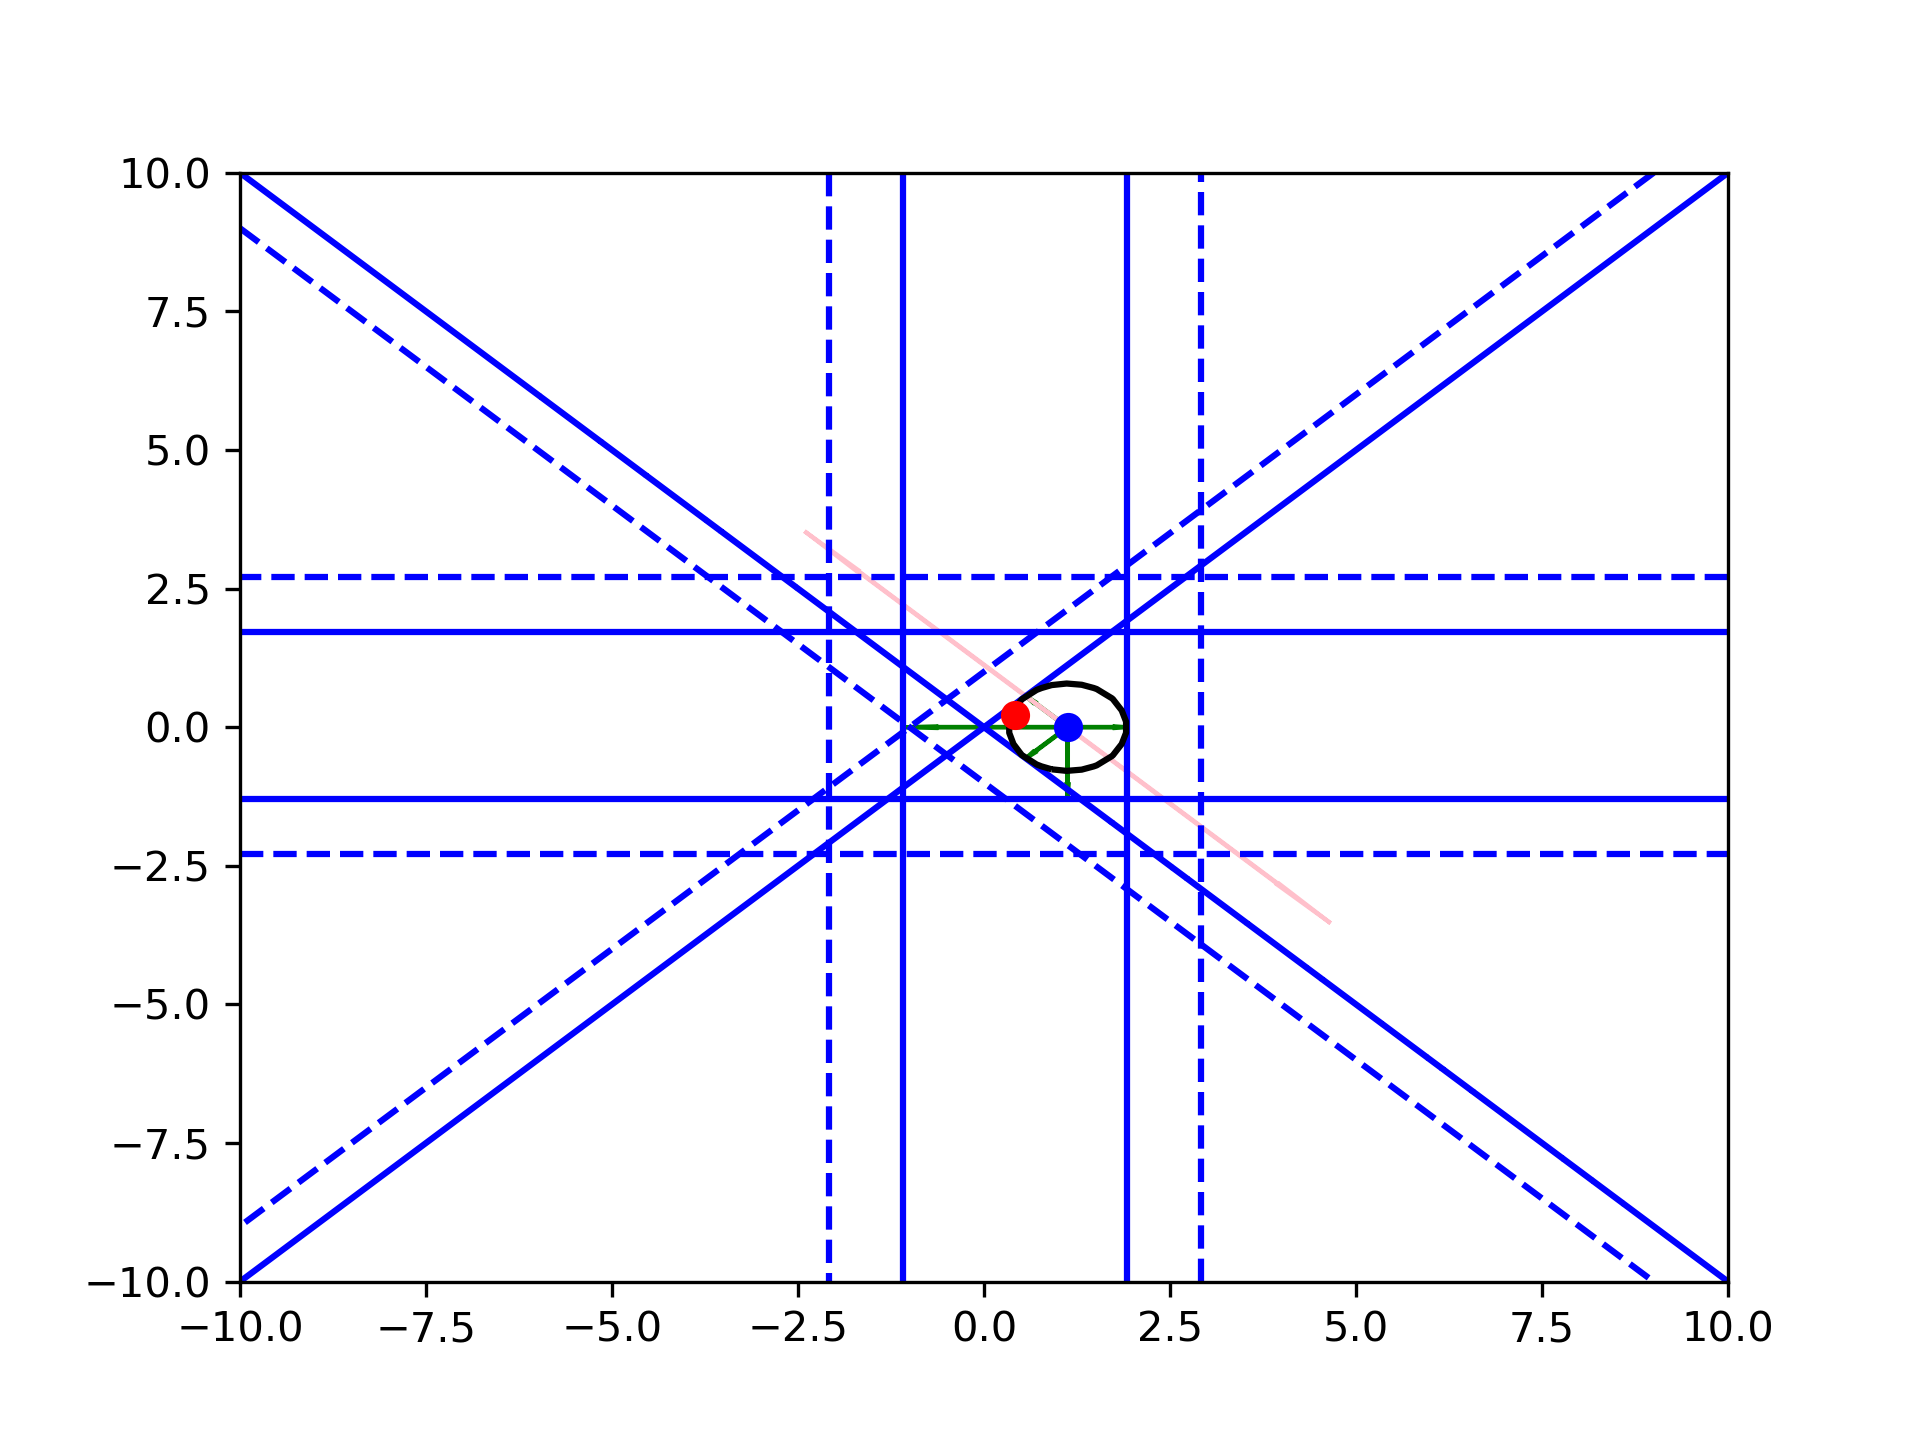
\includegraphics[scale=0.4]{images/run_away_2.png}
    \caption{
%     	\emph{Short:} Why only considering the nearest constraint is not sufficient. 
%     	\emph{Long:} On the left is the starting ellipsoid.
%     	By choosing centers further away from only the nearest constraint, the ellipsoid becomes narrow as another constraint is limiting the length of the second axis.
    Ellipse runs away from the optimizer}
    \label{line_can_run}
\end{figure}




\section{Convergence Discussion}

\subsection{Algorithm Assumptions}

Here, we show convergence for one version of \cref{linearly_constrained_dfo}.
Namely, we choose to satisfy \cref{bluepill} and let $\sampletrk$ have an ellipsoidal shape as described in \cref{sample_region_choices}. 
Also, we will select \cref{search_a_lot} as discussed in \cref{search_region_choices}: namely, $\searchtrk = \outertrk \cap \feasible$.
To do this, we require the following assumptions.

Here, we will let $\domain$ be some open set containing the feasible region: $\feasible \subset \domain$.

\begin{assumption}
\label{the_constraints_are_linear}
The feasible region is described by linear constraints.
That is, we assume that there is an $m \times n$ matrix $\lca$ and vector $\lcb \in \Rm$ such that:
\begin{align*}
\feasible = \left\{x \in \Rn \bigg | \lca x \le \lcb \right\}
\end{align*}
\end{assumption}

\begin{assumption}
\label{lipschitz_gradient}
The function $f$ is differentiable and its gradient $\nabla f$ is Lipchitz continuous with constant $\lipgrad > 0$ in $\domain$.
That is,
\begin{align}
\|\nabla f(x) - \nabla f(y)\| \le \lipgrad \|x - y\| \quad \forall x, y \in \domain.
\end{align}
\end{assumption}

\begin{assumption}
\label{for_fully_quadratic}
\label{lipschitz_hessian}
The function $f$ has Lipschitz continuous hessian with constant $\liphess > 0$ in $\domain$.
That is,
\begin{align}
\left\|\nabla^2 f(x) - \nabla^2 f(y)\right\| \le \liphess \left\|x - y\right\| \quad \forall x, y \in \domain.
\end{align}
\end{assumption}

\begin{assumption}
\label{lower_bound}
The function $f$ is bounded below over $\domain$.
That is,
\begin{align}
f(x) \ge \fmin \quad \forall x \in \domain.
\end{align}
\end{assumption}


\begin{assumption}
\label{uniformly_bounded_hessians_of_mf}
The Hessian's of $\mfk$ are uniformly bounded at each iterate. That is, there exists a constant $\beta \ge 1$ such that 
\begin{align}
\left\|\nabla^2 \mfk\left(\xk\right)\right\| \le \beta - 1\quad \forall k \ge 0.
\end{align}
\end{assumption}

% \begin{assumption}
% \label{accuracy_assumption}
% There exists a constant $\delta_g$ such that 
% \begin{align}
% \|\nabla m_k\left(\xk\right) - \nabla f\left(\xk\right)\| \le \delta_g \dk \;\forall k \ge 0.
% \end{align}
% \end{assumption}

\begin{assumption}
\label{interior_point}
There exists a point $\bar x$ within the interior of the feasible region.
Namely, using $\lca$ and $\lcb$ from \cref{the_constraints_are_linear}:
\begin{align}
\lca \bar x < \lcb.
\end{align}
\end{assumption}

\label{linear_convergence_discussion}


\subsection{Required Assumptions}

If the tolerances $\tau_{\chi} = 0$ and $\tau_{\Delta} = 0$ are set to zero, \cref{linearly_constrained_dfo} is a particular implementation of the algorithm presented in \cite{doi:10.1080/10556788.2015.1026968}.
This means we only need to satisfy the requirements detailed in their convergence analysis.
For your convenience, we duplicate these assumptions.
\begin{itemize}
\item[$H_0$] The efficiency condition \cref{efficiency} is satisfied.
\item[$H_1$] The function $f$ is differentiable and its gradient $\nabla f$ is Lipchitz continuous with constant $L > 0$ in $\domain$.
\item[$H_2$] The function $f$ is bounded below over $\domain$.
\item[$H_3$] The matrices $H_k$ are uniformly bounded. That is, there exists a constant $\beta \ge 1$ such that $\|\nabla^2 \mfk\| \le \beta - 1$ for all $k \ge 0$.
\item[$H_4$] There exists a constant $\delta_g$ such that $\left\|\nabla m_k\left(\xk\right) - \nabla f\left(\xk\right)\right\| \le \delta_g \dk$ for all $k \ge 0$.
\end{itemize}

$H_0$ can be satisfied within our algorithm by selecting the Generalized Cauchy Point \cite{Conn:2000:TM:357813} to solve the trust region subproblem.
Notice that $H_1$, $H_2$, and $H_3$  are kept as hypothesis within our algorithm.
This leaves $H_4$, which is the topic of \cref{satisfying_accuracy}.
However, first we show a way of using a more straightforward version of $H_3$ in \cref{simpler_h3}.

\subsection{Satisfying these assumptions}

\subsubsection{Simplified Third Hypothesis}
\label{simpler_h3}
First, we show that \cref{uniformly_bounded_hessians_of_f} can be used instead of \cref{uniformly_bounded_hessians_of_mf} under some restrictions.
Namely, for this to be true, we also first assume:
\begin{assumption}
\label{delta_max}
There exists a $\dmax > 0$ such that $\dk \le \dmax$ for all $k \ge 0$.
\end{assumption}

With this modest assumption, we can make the assumptions more straightforward by replacing \cref{uniformly_bounded_hessians_of_mf} with \cref{uniformly_bounded_hessians_of_f}:

\begin{assumption}
\label{uniformly_bounded_hessians_of_f}
The Hessian's of $f$ are uniformly bounded at each iterate. That is, there exists a constant $\beta \ge 1$ such that
\begin{align*}
\left\|\nabla^2 f\left(\xk\right)\right\| \le \beta - 1\quad \forall k \in \naturals
\end{align*}
\end{assumption}


This is the result of the following lemma:
\begin{lemma}
\label[lemma]{replacing_h3}
Suppose that \cref{lipschitz_hessian}, \cref{delta_max}, and \cref{uniformly_bounded_hessians_of_f} hold.
Let $\mfk$ is a quadratic model of $f$ over $B_{\infty}(\xk, \dk)$  as in \cref{quadratic_errors} for each $k \in \naturals$.
Then \cref{uniformly_bounded_hessians_of_mf} is also satisfied.
\end{lemma}

\begin{proof}
By \cref{uniformly_bounded_hessians_of_f}, we can choose $\beta_1 \ge 1$ to be such that for all $k \in\naturals$:
\begin{align*}
\left\|\nabla^2 f\left(\xk\right) \right\| \le \beta_1 - 1.
\end{align*}
% \cref{model_improving_algorithm},
Because $\mfk$ are fully quadratic by \cref{lipschitz_hessian}, we know that \cref{introduction_3_1} is satisfied.
Thus, we can apply \cref{quadratic_errors} to see that \cref{error_in_hessian} is satisfied.
Combining this with \cref{delta_max} we see that
\begin{align*}
\left\|\nabla^2 f\left(\xk\right) - \nabla^2 m_f\left(\xk\right) \right\| \le \kappa_{h} \dk \le \kappa_{h} \Delta_{\text{max}}
\end{align*}
Defining $\beta_2 = \kappa_{h} \Delta_{\text{max}} + \beta_1 \ge 1$, we see that
\begin{align*}
\left\|\nabla^2 m_{f}\left(\xk\right)\right\| \le \left\|\nabla^2 m_{f}\left(\xk\right) - \nabla^2 f\left(\xk\right)  \right\| + \left\|\nabla^2 f\left(\xk\right) \right\|
\le \beta_2 - 1 .
\end{align*}
\end{proof}

% For any $x \in \feasible$, we have that the set of gradients of active constraints is linearly independent. That is, the vectors $\{\nabla c_i(x) |  \forall i \in \activei(x)\}$ is linearly independent.


\subsubsection{Satisfying the Accuracy Assumption}
\label{satisfying_accuracy}
The only remaining assumption is the accuracy condition $H_4$.

Because the ellipsoid we construct must be feasible with respect to both the trust region and the constraints,
we simplify notation by creating a matrix $\lctra$ and vector $\lctrb$ from $\lca$ and $\lcb$ defined in \cref{the_constraints_are_linear} as follows:
\begin{align}
\polyk = \{x \in \Rn | \; \lca x \le \lcb, \|x - \xk\|_{\infty} \le \dk \} \label{polyhedron_k} 
= \{x \in \Rn | \lctra x \le \lctrb, \|{\lctra}_i\| = 1 \}.
\end{align}
This is the normalized polyhedron formed by adding the trust region constraints for iteration $k$ to the problem constraints.

As discussed in \cref{ellipsoidal_lambda}, we know that if the condition number of $\qk$ is bounded, 
we can map a poised set over the unit ball to $\sampletrk$.
However, we must also ensure that we are always able to find a feasible ellipsoid.
Although it is not always possible to find a feasible ellipsoid that contains the current iterate,
we can find a feasible ellipsoid that only needs to be scaled by a constant to do so.
This ellipsoid must satisfy the following conditions:

\begin{definition}
\label{define_suitable_ellipsoid}
An ellipsoid $\ellipsek$ determined by a positive definite, symmetric matrix  $\qk$, a center $\ck \in \Rn$, and a radius $\sdk > 0$
is said to be a \textbf{suitable ellipsoid} for iteration $k$ if all of the following are satisfied:
\begin{itemize}
\item[1.] The ellipsoid $\ellipsek = \left\{x \in \Rn \bigg| \left(x - \ck\right)^T\qk\left(x - \ck\right) \le \frac 1 2 \sdk^2 \right\}$ 
satisfies $\ellipsek \subseteq \polyk$ as defined in \cref{polyhedron_k}
\item[2.] The ellipsoid $\scaledellipsek = \left\{x \in \Rn \bigg | \left(x - \ck\right)^T\qk\left(x - \ck\right) \le  \sdk^2 \right\}$ satisfies $\xk \in \scaledellipsek$.
\item[3.] $\condition \left(\qk\right)$ is bounded independently of $k$.
\end{itemize}
\end{definition}

The active constraints at any point will be denoted by
\begin{align}
\activei(x) = \{1 \le i \le m | c_i(x) = 0 \Leftrightarrow {\lca}_ix = {\lcb}_i \} \label{define_activei}
\end{align}

It will be convenient to use a feasible direction with respect to the active constraints at a given point.
To this end, let $\lca$ be defined by \cref{the_constraints_are_linear} and $\mathcal S \subseteq \{1, \ldots, m\}$ be arbitrary.
Define:
\begin{align}
\alphaone (\mathcal S) = \begin{cases}
\argmax_{\|u\| = 1} \min_{i \in \mathcal S} -u^T{\lca}_i & \text{if} \; \mathcal S \ne \emptyset \\
\emptyset & \text{if} \; \mathcal S = \emptyset
\end{cases} \label{define_alpha_one} \\
\alphatwo(\mathcal S) = \begin{cases}
\max_{\|u\| = 1} \min_{i \in \mathcal S} -u^T{\lca}_i & \text{if} \; \mathcal S \ne \emptyset \\
1 & \text{if} \; \mathcal S = \emptyset
\end{cases} \label{define_alpha_two}\\
\alphathree(x) = \alphatwo\left(\activei(x)\right) \label{define_alpha_three} \\
\alpha_k =  \alphathree\left(\xk\right) \label{define_alpha_k} \\
\uk \in  \alphaone\left(\activei\left(\xk\right)\right) \label{define_u_k}
\end{align}
Here, $\alphathree$ is a set of directions that hopefully head away from each of the active constraints at a point.

Throughout, we will use a couple different cones, which can be described here
\begin{align}
\mathcal C(\alpha, d, c) = \left\{x \in \Rn | \quad x = c + t d + s, s^Td= 0, t \ge 0, \|s\| \le \alpha t\right\} \\
\unshiftedcone = \mathcal C(\alpha_k, \uk, \xk) = \{x \in \Rn | \quad x = \xk + t \uk+ s, s^Tu^{\star} = 0, t \ge 0, \|s\| \le \alpha_k t\} \label{defineunshiftedcone} \\
\shiftedcone = \mathcal C(\alpha_k, e_1, 0) =  \{x = (t, s)^T \in \Rn, t \in \mathbb R_{\ge 0}, s \in \mathbb R^{n-1} |\quad \|s\| \le \alpha_k t \} \label{defineshiftedcone}
\end{align}

We will use the following mapping to go between these cones:
\begin{align}
\rotk = 2\frac{(e_1 + \uk)(e_1 +\uk)^T}{(e_1 +\uk)^T(e_1 +\uk)} - \boldsymbol I \label{define_r} \\
T_k(x) = \rotk\left(x - \xk\right) \label{define_affine_mapping}
\end{align}

Finally, the following is a useful function for defining ellipsoids:
\begin{align}
f_{e}(\alpha, \delta, r; x) = (x - \delta e_1)^T\begin{pmatrix}
1 & \boldsymbol0^T \\
\boldsymbol 0 & \alpha^{-2} \boldsymbol I \\
\end{pmatrix}(x - \delta e_1) - r \label{define_ellipsoid_function}
\end{align}


\begin{lemma}
\label[lemma]{alphas_are_positive}
Let $\alphathree$ be defined by \cref{define_alpha_three}.
Suppose that \cref{the_constraints_are_linear} and \cref{interior_point} hold.

Then, $1 \ge \alphathree(x_0) > 0$ for any $x_0 \in \feasible$. 
\end{lemma}

\begin{proof}
Let $x_0 \in \feasible$, and let $\activei$ be defined by \cref{define_activei}.
If $\activei(x_0) = \emptyset$, then $\alphathree(x_0) = 1 > 0$.
Otherwise, let $i \in \activei(x_0)$, so that $c_i(x_0) = 0$.
% We know that for each $i \in \activei(x_0)$ both $c_i(x_0) = 0$ and $c_i(\bar x) < 0$.
% subtract the equations: $G_i^T \bar x < g_i$ and $G_i^T  x_0 = g_i$ to find
Because $c_i$ is convex from \cref{the_constraints_are_linear}, we know that if $\bar x$ is defined as in \cref{interior_point}, then
\begin{align*}
c_i(\bar x) \ge c_i(x_0) + \nabla c_i(x_0)^T(\bar x - x_0)
\Longrightarrow \nabla c_i(x_0)^T(\bar x - x_0) \le c_i(\bar x) - c_i(x_0) = c_i(\bar x) < 0
\end{align*}
Using \cref{polyhedron_k}, we can write this as
\begin{align*}
-{\lca}^T_i\frac {\bar x - x_0}{\|\bar x - x_0\|} > 0  \Longrightarrow \min_{i \in \activei(x_0)} -{\lca}_i^T\frac {\bar x - x_0}{\|\bar x - x_0\|} > 0.
\end{align*}
Using this along with definitions of $\alphaone$, $\alphatwo$, and $\alphathree$ in \cref{define_alpha_one}, \cref{define_alpha_two}, and \cref{define_alpha_three}; we see
\begin{align*}
\alphathree(x_0) = \alphatwo\left(\activei(x_0)\right) = \max_{\|u\| = 1} \min_{i \in \activei(x_0)} -{\lca}_i^Tu
\ge \min_{i \in \activei(x_0)} - {\lca}_i^T\frac {\bar x - x_0}{\|\bar x - x_0\|} > 0.
\end{align*}

We know that $\alphathree(x_0) \le 1$ because it is the dot product of two vectors of length one:
if $\|u\| = 1$, then $\left|u^T {\lca}_i\right|^2 \le \|u\|\|{\lca}_i\| = 1$ by Cauchy–Schwarz.

\end{proof}

\begin{lemma}
\label[lemma]{alphas_are_bounded}
Let $\alpha_k$ be defined by \cref{define_alpha_k}.

Suppose that \cref{the_constraints_are_linear} and \cref{interior_point} hold.

There exists an $\epsilon_{\alpha} > 0$ such that $\alpha_k \ge \epsilon_{\alpha} \; \forall \; k \in \naturals$.
\end{lemma}
\begin{proof}
Let $\activei$ be defined by \cref{define_activei}.
Because there are only $m$ constraints, each $\activei(x)$ is one of the only $2^m$ subsets of  $\{1, 2, 3, \ldots, m\}$.
This means that $\alphaone$, $\alphatwo$, and $\alpha_k$ as defined by \cref{define_alpha_one}, \cref{define_alpha_two}, and \cref{define_alpha_k} can only take on at most $1 + 2^m$ values.
By \cref{alphas_are_positive}, we know that each of these values must be positive.
Thus, we are free to choose $\epsilon_{\alpha}$ to be the smallest of these values.
\end{proof}

\begin{lemma}
\label[lemma]{trivial_ellipsoid_exists}
Let $\activei$ be defined by \cref{define_activei}.

If $\activei = \emptyset$ during iteration $k$, then there exists a suitable ellipsoid for iteration $k$ according to \cref{define_suitable_ellipsoid}.
\end{lemma}
% $\epsilon > 0$, $c \in \Rn$  and a positive definite, symmetric matrix $Q$, 
\begin{proof}
If $\activei = \emptyset$, then we are free to select $\ck = \xk, \qk = I$, and $\sdk$ smaller than the distance to the nearest constraint:
$\sdk \le  \min_{i \in [m]} {\lcb}_i - \left({\lca}_i\right)^T\xk$.
Because $E_k$ is then a sphere with radius less than the distance to the nearest constraint, $E \subseteq P$.
Because the sphere $\hat E_k$ is centered at $\xk$, $\xk \in \hat E_k$.
Also, $\condition(\qk) = 1$.
\end{proof}




\begin{lemma}
\label[lemma]{unshiftedconeisfeasible}
Let $\unshiftedcone$ and $\polyk$ be defined by \cref{defineunshiftedcone} and \cref{polyhedron_k}.
Suppose that \cref{the_constraints_are_linear} holds.

The set $\unshiftedcone$ is feasible with respect to the active constraints of $\polyk$ at $\xk$.
\end{lemma}

\begin{proof}
Note that the trust region boundary cannot be active at $\xk$ as $\dk > 0$.
Let $\activei$, $\alpha_k$, and $\uk$ be defined by \cref{define_activei}, \cref{define_alpha_k}, \cref{define_u_k} and
$\lca$ and $\lcb$ be defined by \cref{the_constraints_are_linear}.
Let $y = \xk + t\uk + s \in \unshiftedcone$ and $i \in \activei\left(\xk\right)$ be arbitrary.
Then,
\begin{align*}
{\lca}_{i}^Ty - {\lcb}_{i} = {\lca}_{i}^T(t\uk + s) = {\lca}_{i}^Ts + t {\lca}_{i}^T\uk \le \|s\| - \alpha_k t \le 0.
\end{align*}
\end{proof}




\begin{lemma}
\label[lemma]{shifted_ellipsoid_in_cone}
Let $\shiftedcone, f_e, \alpha_k$ be defined as in \cref{defineshiftedcone}, \cref{define_ellipsoid_function}, \cref{define_alpha_k}.
Then, for all $\delta > 0$, the ellipsoid
\begin{align}
\left\{x \in \Rn | f_e(\alpha_k, \delta, \frac 1 2 \delta^2; x) \le 0 \right\} \subseteq \shiftedcone.
\end{align}
\end{lemma}

\begin{proof}
Suppose that $x \in \left\{x \in \Rn | f_e(\alpha_k, \delta, \frac 1 2 \delta^2; x) \le 0 \right\}$, then
\begin{align*}
f_e(x) \le 0 \Longrightarrow 
(x - \delta e_1)^T\begin{pmatrix}
1 & \boldsymbol0^T \\
\boldsymbol 0 & \alpha_k^{-2} \boldsymbol I \\
\end{pmatrix}(x - \delta e_1) \le \frac 1 2 \delta^2 
\Longrightarrow (t - \delta)^2 + \frac {1} {\alpha_k^2} \|s\|^2 \le \frac 1 2 \delta^2 \\
\Longrightarrow \|s\|^2 \le \alpha_k^2 \left[\frac 1 2 \delta^2 - (t - \delta)^2\right] 
= \alpha_k^2 \left[t^2 - 2(t - \frac 1 2 \delta)^2 \right] \le \alpha_k^2t^2
\Longrightarrow \|s\| \le \alpha_k t.
\end{align*}
Thus, $x \in\shiftedcone$.
\end{proof}


\begin{lemma}
\label[lemma]{linear_mapping_works}
Let $\rotk$, $T_k$, $\unshiftedcone$, $\shiftedcone$ be defined as in
\cref{define_r}, \cref{define_affine_mapping}, \cref{defineunshiftedcone}, \cref{defineshiftedcone}.
Then $T_k(\unshiftedcone) = \shiftedcone$.
% and $T_k^{-1}(\shiftedcone) = \unshiftedcone$
\end{lemma}

\begin{proof}
Observe that $\rotk e_1 = \uk$, $\rotk \uk = e_1$, $\det(\rotk) = 1$, and 
$\rotk \rotk ^T = \rotk ^T\rotk = I$

Suppose that $x \in \unshiftedcone$.
Then there exists $t \ge 0$ and $s \in \Rn$ such that $x = \xk + t \uk+ s$ where $s^T \uk = 0$ and $\|s\| \le \alpha_k t$.
Then $T_k(x) = t\rotk\uk + \rotk s = te_1 + \rotk s$.
Observe that $(Rs)_1 = (\rotk s)^Te_1 = s^T\rotk^T(\rotk \uk) = s^T \uk = 0$.
Hence,
$T_k(x) = \begin{pmatrix}
t \\
\sigma
\end{pmatrix}$ where $\sigma \in \mathbb R ^ {n-1}$ satisfies $\|\sigma\| = \|s\| \le \alpha t$.
Thus, $T_k(x) \in \shiftedcone$.
Conversely, if $\begin{pmatrix}
t \\
\sigma
\end{pmatrix} \in \shiftedcone$, then let
$s = \rotk^T\begin{pmatrix}
0 \\
\sigma
\end{pmatrix}$
to see that
$x = T_k^{-1}\left(\begin{pmatrix}
t \\
\sigma
\end{pmatrix} \right)= \rotk^T\left(t e_1 + \begin{pmatrix}
0 \\
\sigma
\end{pmatrix}\right) = t \uk + s$ where 
$\|s\| = \|\sigma\| \le \alpha t$.
Hence $T_k^{-1}\left(\begin{pmatrix}
t \\
\sigma
\end{pmatrix}\right) \in \unshiftedcone$.
\end{proof}



\begin{lemma}
\label[lemma]{ellipsoid_fits}
Let $\rotk$, $T_k$, $\unshiftedcone$, $\shiftedcone$, $\polyk$ be defined as in
\cref{define_r}, \cref{define_affine_mapping}, \cref{defineunshiftedcone}, \cref{defineshiftedcone}, \cref{polyhedron_k}.
Suppose that \cref{the_constraints_are_linear} holds.

For each iteration $k$, there exists a $\deltaf > 0$ such that the ellipsoid
\begin{align}
\ellipsek = \left\{x \in \Rn \bigg | f_e\left(\deltaf, \frac 1 2 \deltaf^2, \alpha_k, T_k(x)\right) \le 0\right\} \label{definefeasibleellipsoid}
\end{align}
satisfies $\ellipsek \subseteq \polyk$.
\end{lemma}

\begin{proof}
Let $L$ be the shortest distance from $\xk$ to any point on a non-active constraint. 
Define $\alpha' = \sqrt{\left(1 + \alpha_k^2 \right) \left(1 + \frac 1 {\sqrt{2}}\right)}$, and let $\deltaf = \frac 1 {\alpha'} L$.
We see that if $x \in \ellipsek$,
then by \cref{shifted_ellipsoid_in_cone} we have that $T_k(x) = \begin{pmatrix}t\\ \sigma\end{pmatrix} \in \shiftedcone$ for some $\sigma \in \mathbb R^{n-1}$, and
\begin{align*}
(x - \deltaf e_1)^T\begin{pmatrix}
1 & \boldsymbol0^T \\
\boldsymbol 0 & \alpha_k^{-2} \boldsymbol I \\
\end{pmatrix}(x - \deltaf e_1) \le \frac 1 2 \deltaf^2 \\
\Longrightarrow (t - \deltaf)^2 + \frac {1} {\alpha_k^2} \|\sigma\|^2 \le \frac 1 2 \deltaf^2
\Longrightarrow (t - \deltaf)^2 \le \frac 1 2 \deltaf^2
\Longrightarrow t \le \left(1 + \frac 1 {\sqrt{2}}\right) \deltaf
\end{align*}
so that 
\begin{align*}
\|x\|^2 = t^2 + \|\sigma\|^2 \le \left(1 + \alpha_k^2 \right) t^2 \le \left(1 + \alpha_k^2 \right) \left(1 + \frac 1 {\sqrt{2}}\right) \deltaf^2 = {\alpha'}^2 \deltaf^2 \\
\Longrightarrow \|x\| \le \alpha' \deltaf \le L
\end{align*}
Thus, all points within $\ellipsek$ are closer than the nearest point of a non-active constraint.
Combine this with \cref{unshiftedconeisfeasible} to see that $\ellipsek \subseteq \polyk$.
\end{proof}



\begin{lemma}
\label[lemma]{ellipsoid_includes_origin}
For some iteration $k$, let $\rotk$, $T_k$, $\unshiftedcone$, $\shiftedcone$, $\polyk$ be defined as in
\cref{define_r}, \cref{define_affine_mapping}, \cref{defineunshiftedcone}, \cref{defineshiftedcone}, \cref{polyhedron_k}.
Also, let $\deltaf > 0$ be defined as in \cref{ellipsoid_fits}.

The ellipsoid
\begin{align}
\scaledellipsek  = \left\{x \in \Rn | f_e\left(\deltaf, \deltaf^2, \alpha_k, T_k(x)\right) \le 0\right\} \label{definescaledfeasibleellipsoid}
\end{align}
satisfies $\xk \in \scaledellipsek$.
\end{lemma}

\begin{proof}
We have that
\begin{align*}
f_e(\deltaf, \deltaf^2, \alpha_k, T_k\left(\xk\right) ) =  
f_e(\deltaf, \deltaf^2, \alpha_k, 0 ) =  
(0 - \deltaf e_1)^T\begin{pmatrix}
1 & \boldsymbol0^T \\
\boldsymbol 0 & \alpha_k^{-2} \boldsymbol I \\
\end{pmatrix}(0 - \deltaf e_1) = \deltaf^2 \le \deltaf^2.
\end{align*}
\end{proof}








% 
% 
% 
% 
% We will first define the ellipsoid and show some of its properties within the transformed space $C_2$ before mapping it to $C_1$.
% To this end, fix an arbitrary $\delta > 0$ and let 
% $f_{e}(x): \Rn \to \reals $ be defined by 
% \begin{align}
% f_{e}(x) = (x - \delta e_1)^T\begin{pmatrix}
% 1 & \boldsymbol0^T \\
% \boldsymbol 0 & \alpha^{-2} \boldsymbol I \\
% \end{pmatrix}(x - \delta e_1) - \frac 1 2 \delta^2
% \label{define_ellipsoid_function}
% \end{align} 
% and consider the ellipsoid $E_1 = \{x | f_{e}(x) \le 0\}$.
% We will show that $E_1 \subseteq C_2$.
% To this end, suppose $x = (t, s) \in E_1$.
% Firstly, note that
% \begin{align*}
% 2\big(t - \frac {\delta} 2\big)^2 \ge 0
% \Longrightarrow 2t\delta - \frac 1 2 \delta^2 \le 2t^2 
% \Longrightarrow \frac 1 2 \delta^2 - (t - \delta)^2 \le t^2. 
% \end{align*}
% \Longrightarrow \frac 1 2 \delta^2 -t^2  + 2t\delta - \delta^2 \le t^2 \\
% \Longrightarrow 0 \le t^2 - t\delta + \frac 1 4 \delta^2
%  \Longrightarrow 0 \le 2t^2 - 2t\delta + \frac 1 2 \delta^2\\

% We choose this mapping because if $x = x_0 + t u^{\star} + s \in C_1$,
% then $\|s\|\le \alpha t \Leftrightarrow \|Rs\| \le \alpha t$ and $0 = s^Tu^{\star} = s^T R^T R u^{\star} = (Rs)^T e_1$ imply that 
% $R(x - x_0 - \delta u^{\star}) = t Ru^{\star} + Rs = t e_1 + Rs \in C_2$.
% Thus, the affine mapping $T : \Rn \to \Rn$ defined by $T(x) = R(x - x_0 - \delta u^{\star})$ maps $C_1$ to $C_2$.
% Conversely, the same arguments show that $T^{-1}(x) = R^Tx + x_0 + \delta u^{\star}$ maps $C_2$ to $C_1$.

%  \in SO(n)
% u = [3957; 6294.9]
% u = u / norm(u)
% e = [1; 0.0]
% a = e + u
% r = 2 * a * a' / (a' * a) - eye(2)
% r * e
% r * u


% 
% Having proven that $E_1 \subseteq C_2$, it follows that $T^{-1}(E_1) \subseteq C_2$.
% However, $T^{-1}(E_1) = \{ x \in \Rn | (x - \delta u^{\star})^TQ(x-\delta u^{\star} \le \frac 1 2 \epsilon\}$ where

% 
% \begin{align*}
% E_2 = \bigg \{x \bigg | (x - x_0 - \delta u^{\star})^T\bigg(R^T\begin{pmatrix}
% 1 & \boldsymbol0^T \\
% \boldsymbol 0 & \alpha^{-2} \boldsymbol I \\
% \end{pmatrix}R\bigg)(x - x_0 - \delta u^{\star}) \le \frac 1 2 \delta^2 \bigg\}.
% \end{align*}
% We know that $x \in E_1 \Leftrightarrow T(x) = R(x - x_0 - \delta u^{\star}) \in E_2 \Longrightarrow T(x) \in C_2 \Longrightarrow x = T^{-1}\left(T(x)\right) \in C_1$.
% Thus, we know that the ellipsoid $E_2$ is contained within the active constraints, and can be scaled by $2$ to include $x_0$.

\begin{lemma}
\label[lemma]{nontrivial_ellipsoid_exists}
Let $\alpha_k$ be defined by \cref{define_alpha_k}.
Suppose that \cref{the_constraints_are_linear} holds.

For iteration $k$, if $\alpha_k > 0$, then there exists a suitable ellipsoid for iteration $k$ according to \cref{define_suitable_ellipsoid}.
\end{lemma}

\begin{proof}
Let 
$\rotk$,
be defined as in
\cref{define_r}
.
Also, let
$\deltaf$, $\scaledunshiftedellipsoid$
be defined as in 
\cref{definefeasibleellipsoid}
\cref{definescaledfeasibleellipsoid}
.

Let
\begin{align*}
\qk = \rotk^T\begin{pmatrix}
1 & \boldsymbol0^T \\
\boldsymbol 0 & \alpha_k^{-2} \boldsymbol I \\
\end{pmatrix}\rotk \\
c_k = \xk - \deltaf \uk \\
\epsilon = \delta^2 
\end{align*}

By \cref{ellipsoid_fits}, we know that $\unshiftedellipsoid \subseteq \polyk$.
By \cref{ellipsoid_includes_origin}, we know that $\xk \in \scaledunshiftedellipsoid$ .
The condition number of $\condition(\qk) = \frac{\max\{1, \alpha_k^{-2}\}}{\min\{1, \alpha_k^{-2}\}} = \alpha_k^{-2}$.
This is because $\det(\rotk) = 1$ means the condition number of $\qk$ is not affected $\rotk$.
\end{proof}



\begin{boxedcomment}
I think we no longer use this result...
\end{boxedcomment}

We use the following result shown \cite{BillupsLarson2013}, Corollary 4.7.
We restate the theorem here, with the simplication that $f$ is deterministic function:

\begin{assumption}
\label{fully_quadratic_assumption}
Suppose that a set $S$ and a radius $\dmax$ are given.
Assume that $f$ is twice continuously differentiable with Lipshcitz continuous Hessian in an open domain containing the $\dmax$ neighborhood
$\cup_{x \in S} B(x; \dmax)$ of the set $S$.
\end{assumption}

\begin{lemma}
\label[lemma]{larson_change_radius} 
Let $Y$ be a poised set of $p$ points, and let $R = \max_{i}\|y^i - y^0\|$.
Let $f$ satisfy \cref{fully_quadratic_assumption} over some convex set $\Omega$, and let $m(x)$ denote the quadratic model of $f$ using \cref{reg}.
If $f$ is a Lipschitz continuous function with Lipschitz constant $L_g$, and $m_f(x)$ is a quadratic model of $f$.
Then, there exist constrants $\Lambda_1, \Lambda_2, \Lambda_3$ independent of $R$ such that for all $x \in B(y^0, R)$,
\begin{align*}
\|f(x) - m_f(x)\| \le 4\Lambda_1 R^3L \sqrt{p+1} \\
\|\nabla f(x) - \nabla m(x)\| \le 4\Lambda_2R^2  L \sqrt{p+1} \\
\|\nabla^2 f(x) - \nabla^2 m(x)\| \le 4\Lambda_3  RL \sqrt{p+1}
\end{align*}
\end{lemma}

We can now satisfy the accuracy condition.


\begin{boxedcomment}
This has a forward lemma reference to a lemma in Chapter 4.
\end{boxedcomment}

\begin{theorem}
\label{linear_accuracy_is_satisfied}
Suppose that \cref{the_constraints_are_linear} and \cref{interior_point} hold.

The accuracy condition \cref{accuracy} is satisfied for each iterate $k$.
Namely, there exists $\kappa_{g} > 0$ such that 
\begin{align*}
\left\|\nabla m_f\left(\xk\right) - \nabla f\left(\xk\right)\right\| \le \kappa_g \dk \quad \forall k \in \naturals.
\end{align*}
\end{theorem}

\begin{proof}
Fix an iterate $k$.
If there are no active constraints, then we can use \cref{trivial_ellipsoid_exists} to construct a suitable ellipsoid.
Otherwise, we can use \cref{alphas_are_bounded} to satisify the conditions of \cref{nontrivial_ellipsoid_exists}.
% $P = \{x \in \Rn |  \nabla c\left(\xk\right)^T x \le c\left(\xk\right), \xk - \dk \le x \le \xk + \dk \}$.
This provides two ellipsoids:
\begin{itemize}
\item $\unshiftedellipsoid = \{x \in \Rn | \left(x - c^{(k)} \right)^T \qk \left(x - c^{(k)}\right) \le \frac 1 2 {\delta_k}^2 \}$, $\unshiftedellipsoid \subset \polyk$.
\item $\scaledunshiftedellipsoid = \{x \in \Rn | \left(x - c^{(k)}\right)^T \qk \left(x - c^{(k)}\right) \le {\delta_k}^2 \}$, $\xk \in \scaledunshiftedellipsoid$.
\end{itemize}
As in \cref{shifted_ellipsoid}, we can give $Q^{(k)} = LD^2L^T$ its eigen-decomposition, and define $\delta = \max_{x \in \unshiftedellipsoid} \|x - \mu^{(k)}\|$, 
so the transformation $T(x) = \delta D L^T(x - \mu^{(k)})$ maps $E^{(k)}$ to the $\delta$ ball.
As also described in \cref{shifted_ellipsoid}, we  create shifted functions
$\hat {m}_f(u) = m_f(T^{-1}(u))$ and
$\hat f (u) = f(T^{-1}(u))$.
After using \cref{model_improving_algorithm} to choose sample points, we know by \cref{quadratic_errors} that there exists a constants $\kappa_f, \kappa_g, \kappa_h$ such that for all $u \in B(0, \delta)$:
\begin{align*}
\left\| \hat {f}\left(u\right) -  \hat{m}_f\left(u\right) \right\|\le \kappa_f \delta^3 \\
\left\|\nabla \hat {f}\left(u\right) - \nabla \hat{m}_f\left(u\right) \right\|\le \kappa_g \delta^2 \\
\left\|\nabla^2 \hat {f}\left(u\right) - \nabla^2 \hat{m}_f\left(u\right) \right\|\le \kappa_h \delta
\end{align*}
We can then use \cref{change_radius} to conclude that there is another constant $\Lambda_2$ such that for all $u \in B(0, 2\delta)$:
\begin{align*}
\left\|\nabla \hat {f}\left(u\right) - \nabla \hat{m}_f\left(u\right) \right\|\le 4 \Lambda_2 \left(2\delta\right)^2 L \sqrt{p+1} = {\kappa'}_g\delta^2
\end{align*}
where $\kappa_{g}' = 16 \Lambda_2 L \sqrt{p+1}$.
Notice that Lemma 3.1 and Lemma 3.2 within \cite{doi:10.1080/10556788.2015.1026968} show that $\lim_{k\to\infty}\dk = 0$ without requiring the accuracy condition.
This is because Lemma 3.1 assumes that $\dk \le 1$ explicitly, while Lemma 3.2 uses the accuracy of the model's Hessians.
This justifies the use of a $\dmax > 0$, such that $\dk \le \dmax\;\forall k \in \naturals$.
After using  \cref{alphas_are_bounded} to construct an $\epsilon_{\alpha} > 0$ and defining $\kappa''_{g} =  \frac{\kappa'_g}{\epsilon_{\alpha}}\dmax$, we see that
we can use  \cref{shifted_ellipsoid} to conclude that for all $x_0 \in \scaledunshiftedellipsoid$:
\begin{align*}
\left\|\nabla f\left(x_0 \right) - \nabla m_f\left(x_0\right)\right\| \le 
\kappa'_g  \dk^2 \sqrt{\kappa\left(\frac 2 {\delta_k} Q^{(k)}\right)}=  \kappa'_g \sqrt{\alpha_k^{-2}}\dk^2 \le \frac{\kappa'_g}{\alpha_k} \dk\dmax\le \kappa''_g\dk.
\end{align*}
In particular, $\xk \in \scaledunshiftedellipsoid$.
\end{proof}


Notice that although \cref{linear_accuracy_is_satisfied} requires $\delta \le 1$, the authors of  show that $\dk \to 0$ within Lemma 3.1 and Lemma 3.2.
Within Lemma 3.1, $\dk \le 1 $ explicitly. 

\newpage


\section{Results}


\subsection{Sample Problem}
The first test was on a problem with simple constraints and a pathological objective.
We let $f(x) = \epsilon x + (1-\epsilon)(y - \alpha x \sin(\gamma x))^2$ for a fixed constant $\epsilon$, and set the constraints to be
$x_2 \le ax_1$, $x_2 \ge -ax_1$ for a fixed constant $a$.

We summarize the number of function evaluations and iterations taken here:
\tiny
\begin{center}
\begin{longtable}{ c c c c c c c c }
Shape & Search & Num. Segments & Basis & Iterations & Evaluations \\
\hline
                spherical &   anywhere &       &     linear & 159  &   202  &  470 &  630 \\
                spherical &   anywhere &       &  quadratic & 164  &   277  &  467 &  805 \\
                spherical &       none &       &     linear &  77* &   122* &  255 &  387 \\
                spherical &       none &       &  quadratic &  74  &   149  &  250 &  561 \\
                spherical &    segment &     1 &     linear &  74  &   116  &  224 &  413 \\
                spherical &    segment &     1 &  quadratic &  74  &   164  &  224 &  525 \\
                spherical &    segment &     2 &     linear & 164  &   223  &  313 &  503 \\
                spherical &    segment &     2 &  quadratic & 152  &   259  &  313 &  657 \\
  circumscribed ellipsoid &       none &       &     linear &  41  &    50  &   41 &   55 \\
  circumscribed ellipsoid &       none &       &  quadratic &  41  &   104  &   41 &  105 \\
                ellipsoid &   anywhere &       &     linear &  65  &   109  &   67 &  110 \\
                ellipsoid &   anywhere &       &  quadratic &  66  &   170  &   67 &  185 \\
%                ellipsoid &  anywhere* &       &  quadratic &  61  &   157  &   60 &  155 \\
                ellipsoid &       none &       &     linear &  53  &    65  &   50 &   52 \\
                ellipsoid &       none &       &  quadratic &  53  &    88  &   50 &   75 \\
                ellipsoid &    segment &     1 &     linear &  55  &    70  &   58 &   75 \\
                ellipsoid &    segment &     1 &  quadratic &  55  &    97  &   58 &  104 \\
                ellipsoid &    segment &     2 &     linear &  67  &   144  &   68 &  121 \\
                ellipsoid &    segment &     2 &  quadratic &  67  &   196  &   64 &  159 \\
               polyhedral &       none &       &     linear &  37  &    43  &   38 &   46 \\
               polyhedral &       none &       &  quadratic &  37  &    82  &   38 &   89 \\
         scaled ellipsoid &   anywhere &       &     linear &  66  &   103  &   67 &  104 \\
         scaled ellipsoid &   anywhere &       &  quadratic &  68  &   156  &   67 &  169 \\
         scaled ellipsoid &    segment &     1 &     linear &  44  &    65  &   45 &   67 \\
         scaled ellipsoid &    segment &     1 &  quadratic &  44  &    94  &   45 &   93 \\
         scaled ellipsoid &    segment &     2 &     linear &  67  &   125  &   68 &  122 \\
         scaled ellipsoid &    segment &     2 &  quadratic &  67  &   189  &   63 &  146 \\
                  simplex & max volume &       &     linear &  41  &    44  &   41 &   45 \\
                  simplex & max volume &       &  quadratic &  41  &    94  &   41 &   84 \\

%                spherical &   anywhere &       &     linear &   159 &   202 \\
%                spherical &   anywhere &       &  quadratic &   164 &   277 \\
%                spherical &       none &       &     linear &    77* &   122* \\
%                spherical &       none &       &  quadratic &    74 &   149 \\
%                spherical &    segment &     1 &     linear &    74 &   116 \\
%                spherical &    segment &     1 &  quadratic &    74 &   164 \\
%                spherical &    segment &     2 &     linear &   164 &   223 \\
%                spherical &    segment &     2 &  quadratic &   152 &   259 \\
%  circumscribed ellipsoid &       none &       &     linear &    41 &    50 \\
%  circumscribed ellipsoid &       none &       &  quadratic &    41 &   104 \\
%                ellipsoid &   anywhere &       &     linear &    65 &   109 \\
%                ellipsoid &   anywhere &       &  quadratic &    66 &   170 \\
%                ellipsoid &  anywhere* &       &  quadratic &    61 &   157 \\
%                ellipsoid &       none &       &     linear &    53 &    65 \\
%                ellipsoid &       none &       &  quadratic &    53 &    88 \\
%                ellipsoid &    segment &     1 &     linear &    55 &    70 \\
%                ellipsoid &    segment &     1 &  quadratic &    55 &    97 \\
%                ellipsoid &    segment &     2 &     linear &    67 &   144 \\
%                ellipsoid &    segment &     2 &  quadratic &    67 &   196 \\
%               polyhedral &       none &       &     linear &    37 &    43 \\
%               polyhedral &       none &       &  quadratic &    37 &    82 \\
%         scaled ellipsoid &   anywhere &       &     linear &    66 &   103 \\
%         scaled ellipsoid &   anywhere &       &  quadratic &    68 &   156 \\
%         scaled ellipsoid &    segment &     1 &     linear &    44 &    65 \\
%         scaled ellipsoid &    segment &     1 &  quadratic &    44 &    94 \\
%         scaled ellipsoid &    segment &     2 &     linear &    67 &   125 \\
%         scaled ellipsoid &    segment &     2 &  quadratic &    67 &   189 \\
%                  simplex & max volume &       &     linear &    41 &    44 \\
%                  simplex & max volume &       &  quadratic &    41 &    94 \\

\end{longtable}
\end{center}
\normalsize

*The spherical trust region with no search for the center did not converge.

In general, the linear models converge more quickly than quadratic models.
We see that the method with fewest iterations and function evaluations is the linear polyhedral shape.
This is likely due to the fact that the polyhedral shape is allowed to search the entire outer trust region.
This also explains why the circumscribed ellipse and maximum volume simplex also perform well.
%We also notices that with a simple heuristic we were able to improve the ellipse slightly from 170 to 157.
Also, the scaled ellipsoid performs comparably to the unscaled version.

\subsection{Schittkowksi Test Problems}


We tested these algorithms on several problems from the Hot-Schittkowski problem set \cite{Schittkowski:1987:MTE:27135}, \cite{Hock1980}.
We selected the problems that have linear constraints: 21, 24, 25, 35, 36, 44, 45, 76, 224, 231, 232, 250, 251.

% 37 was left out because it proved to be difficult.

We summarize the results here.
\begin{tiny}

\begin{center}
\begin{longtable}{ c c c c c c c c c c }
Algorithm & Prob. & n & Message & N. It. & N. Eval. & Ret. Min. & Min. & Solution & Minimizer \\
\hline
  circumscribed ellipse   &   21  &  2  & converged  &   24  &   71  &  -99.960   &  -99.960   & [2.00,0.00] & [2.00,0.00] \\
         ellipse          &   21  &  2  & converged  &   36  &   96  &  -99.960   &  -99.960   & [2.00,0.00] & [2.00,0.00] \\
    ellipse everywhere    &   21  &  2  & converged  &   24  &   82  &  -99.960   &  -99.960   & [2.00,0.00] & [2.00,0.00] \\
    ellipse segment 1     &   21  &  2  & converged  &   24  &   84  &  -99.960   &  -99.960   & [2.00,0.00] & [2.00,0.00] \\
    ellipse segment 2     &   21  &  2  & converged  &   24  &   85  &  -99.960   &  -99.960   & [2.00,0.00] & [2.00,0.00] \\
        polyhedral        &   21  &  2  & converged  &   26  &   75  &  -99.960   &  -99.960   & [2.00,-0.00] & [2.00,0.00] \\
  circumscribed ellipse   &  224  &  2  &   failed   &   16  &   56  &  -304.000  &  -304.000  & [4.00,4.00] & [4.00,4.00] \\
         ellipse          &  224  &  2  & converged  &   32  &   97  &  -304.000  &  -304.000  & [4.00,4.00] & [4.00,4.00] \\
    ellipse everywhere    &  224  &  2  & converged  &   24  &   94  &  -303.774  &  -304.000  & [3.73,4.27] & [4.00,4.00] \\
    ellipse segment 1     &  224  &  2  & converged  &   24  &   91  &  -303.774  &  -304.000  & [3.73,4.27] & [4.00,4.00] \\
    ellipse segment 2     &  224  &  2  & converged  &   23  &   89  &  -303.774  &  -304.000  & [3.73,4.27] & [4.00,4.00] \\
        polyhedral        &  224  &  2  & converged  &   17  &   64  &  -304.000  &  -304.000  & [4.00,4.00] & [4.00,4.00] \\
  circumscribed ellipse   &  231  &  2  & converged  &   14  &   44  &   0.000    &   0.000    & [1.00,1.00] & [1.00,1.00] \\
         ellipse          &  231  &  2  & converged  &   99  &  193  &   0.000    &   0.000    & [1.00,1.00] & [1.00,1.00] \\
    ellipse everywhere    &  231  &  2  & converged  &  181  &  336  &   0.000    &   0.000    & [1.00,1.00] & [1.00,1.00] \\
    ellipse segment 1     &  231  &  2  & converged  &   78  &  162  &   0.000    &   0.000    & [1.00,1.00] & [1.00,1.00] \\
    ellipse segment 2     &  231  &  2  & converged  &  173  &  321  &   0.000    &   0.000    & [1.00,1.00] & [1.00,1.00] \\
        polyhedral        &  231  &  2  & converged  &   95  &  193  &   0.000    &   0.000    & [1.00,1.00] & [1.00,1.00] \\
  circumscribed ellipse   &  232  &  2  &   failed   &   15  &   35  &   -1.000   &   -1.000   & [3.00,1.73] & [3.00,1.73] \\
         ellipse          &  232  &  2  & converged  &   34  &   91  &   -1.000   &   -1.000   & [3.00,1.73] & [3.00,1.73] \\
    ellipse everywhere    &  232  &  2  & converged  &   41  &  102  &   -1.000   &   -1.000   & [3.00,1.73] & [3.00,1.73] \\
    ellipse segment 1     &  232  &  2  & converged  &   34  &   91  &   -1.000   &   -1.000   & [3.00,1.73] & [3.00,1.73] \\
    ellipse segment 2     &  232  &  2  & converged  &   35  &   95  &   -1.000   &   -1.000   & [3.00,1.73] & [3.00,1.73] \\
        polyhedral        &  232  &  2  & converged  &   15  &   47  &   -1.000   &   -1.000   & [3.00,1.73] & [3.00,1.73] \\
  circumscribed ellipse   &   24  &  2  &   failed   &   15  &   35  &   -1.000   &   -1.000   & [3.00,1.73] & [3.00,1.73] \\
         ellipse          &   24  &  2  & converged  &   34  &   90  &   -1.000   &   -1.000   & [3.00,1.73] & [3.00,1.73] \\
    ellipse everywhere    &   24  &  2  & converged  &   41  &  104  &   -1.000   &   -1.000   & [3.00,1.73] & [3.00,1.73] \\
    ellipse segment 1     &   24  &  2  & converged  &   34  &   91  &   -1.000   &   -1.000   & [3.00,1.73] & [3.00,1.73] \\
    ellipse segment 2     &   24  &  2  & converged  &   35  &   95  &   -1.000   &   -1.000   & [3.00,1.73] & [3.00,1.73] \\
        polyhedral        &   24  &  2  & converged  &   15  &   47  &   -1.000   &   -1.000   & [3.00,1.73] & [3.00,1.73] \\
  circumscribed ellipse   &  250  &  3  &   failed   &   24  &  103  & -3300.000  & -3300.000  & [20.00,11.00,15.00] & [20.00,11.00,15.00] \\
         ellipse          &  250  &  3  & converged  &   53  &  207  & -3300.000  & -3300.000  & [20.00,11.00,15.00] & [20.00,11.00,15.00] \\
    ellipse everywhere    &  250  &  3  &   failed   &   48  &  103  & -3298.196  & -3300.000  & [19.99,10.99,15.02] & [20.00,11.00,15.00] \\
    ellipse segment 1     &  250  &  3  &   failed   &   53  &  112  & -3299.243  & -3300.000  & [19.99,11.00,15.01] & [20.00,11.00,15.00] \\
    ellipse segment 2     &  250  &  3  &   failed   &   54  &  112  & -3299.082  & -3300.000  & [19.99,11.00,15.01] & [20.00,11.00,15.00] \\
    ellipse segment 3     &  250  &  3  &   failed   &   56  &  116  & -3299.504  & -3300.000  & [19.99,11.00,15.00] & [20.00,11.00,15.00] \\
        polyhedral        &  250  &  3  & converged  &   26  &  113  & -3300.000  & -3300.000  & [20.00,11.00,15.00] & [20.00,11.00,15.00] \\
  circumscribed ellipse   &  251  &  3  &   failed   &   20  &   86  & -3456.000  & -3456.000  & [24.00,12.00,12.00] & [24.00,12.00,12.00] \\
         ellipse          &  251  &  3  &   failed   &   10  &   53  & -3454.018  & -3456.000  & [23.55,12.06,12.16] & [24.00,12.00,12.00] \\
    ellipse everywhere    &  251  &  3  &   failed   &   6   &   17  & -3209.710  & -3456.000  & [22.82,13.03,10.79] & [24.00,12.00,12.00] \\
    ellipse segment 1     &  251  &  3  &   failed   &   4   &   13  & -1698.807  & -3456.000  & [21.71,9.21,8.50] & [24.00,12.00,12.00] \\
    ellipse segment 2     &  251  &  3  &   failed   &   6   &   17  & -3210.341  & -3456.000  & [21.49,11.46,13.04] & [24.00,12.00,12.00] \\
    ellipse segment 3     &  251  &  3  &   failed   &   14  &   64  & -3449.803  & -3456.000  & [22.84,12.29,12.29] & [24.00,12.00,12.00] \\
        polyhedral        &  251  &  3  & converged  &   22  &  124  & -3456.000  & -3456.000  & [24.00,12.00,12.00] & [24.00,12.00,12.00] \\
  circumscribed ellipse   &   25  &  3  & converged  &  760  &  1472 &   0.000    &   0.000    & [52.92,24.90,1.52] & [50.00,25.00,1.50] \\
    ellipse everywhere    &   25  &  3  &   failed   &   1   &   1   &   32.835   &   0.000    & [100.00,12.50,3.00] & [50.00,25.00,1.50] \\
    ellipse segment 1     &   25  &  3  &   failed   &   1   &   1   &   32.835   &   0.000    & [100.00,12.50,3.00] & [50.00,25.00,1.50] \\
    ellipse segment 2     &   25  &  3  &   failed   &   1   &   1   &   32.835   &   0.000    & [100.00,12.50,3.00] & [50.00,25.00,1.50] \\
    ellipse segment 3     &   25  &  3  &   failed   &   1   &   1   &   32.835   &   0.000    & [100.00,12.50,3.00] & [50.00,25.00,1.50] \\
        polyhedral        &   25  &  3  & converged  &  1793 &  3396 &   0.000    &   0.000    & [50.94,24.97,1.51] & [50.00,25.00,1.50] \\
  circumscribed ellipse   &   35  &  3  &   failed   &  781  &  1028 &   0.111    &   0.111    & [1.33,0.78,0.44] & [1.33,0.78,0.44] \\
         ellipse          &   35  &  3  & converged  &   28  &  122  &   0.111    &   0.111    & [1.33,0.78,0.44] & [1.33,0.78,0.44] \\
    ellipse everywhere    &   35  &  3  &   failed   &   24  &   82  &   0.113    &   0.111    & [1.36,0.79,0.42] & [1.33,0.78,0.44] \\
    ellipse segment 1     &   35  &  3  &   failed   &   16  &   76  &   0.112    &   0.111    & [1.31,0.79,0.45] & [1.33,0.78,0.44] \\
    ellipse segment 2     &   35  &  3  &   failed   &   16  &   75  &   0.112    &   0.111    & [1.31,0.79,0.45] & [1.33,0.78,0.44] \\
    ellipse segment 3     &   35  &  3  &   failed   &   16  &   77  &   0.112    &   0.111    & [1.31,0.79,0.45] & [1.33,0.78,0.44] \\
        polyhedral        &   35  &  3  & converged  &   14  &  112  &   0.111    &   0.111    & [1.33,0.78,0.44] & [1.33,0.78,0.44] \\
  circumscribed ellipse   &   36  &  3  &   failed   &   19  &   81  & -3300.000  & -3300.000  & [20.00,11.00,15.00] & [20.00,11.00,15.00] \\
         ellipse          &   36  &  3  & converged  &   53  &  202  & -3300.000  & -3300.000  & [20.00,11.00,15.00] & [20.00,11.00,15.00] \\
    ellipse everywhere    &   36  &  3  &   failed   &   63  &  135  & -3299.808  & -3300.000  & [20.00,11.00,15.00] & [20.00,11.00,15.00] \\
    ellipse segment 1     &   36  &  3  &   failed   &   64  &  140  & -3299.951  & -3300.000  & [20.00,11.00,15.00] & [20.00,11.00,15.00] \\
    ellipse segment 2     &   36  &  3  &   failed   &   64  &  133  & -3299.918  & -3300.000  & [20.00,11.00,15.00] & [20.00,11.00,15.00] \\
    ellipse segment 3     &   36  &  3  &   failed   &   65  &  137  & -3299.870  & -3300.000  & [20.00,11.00,15.00] & [20.00,11.00,15.00] \\
        polyhedral        &   36  &  3  & converged  &   22  &  108  & -3300.000  & -3300.000  & [20.00,11.00,15.00] & [20.00,11.00,15.00] \\
  circumscribed ellipse   &   37  &  3  &   failed   &   27  &   98  & -3456.000  & -3456.000  & [24.00,12.00,12.00] & [24.00,12.00,12.00] \\
         ellipse          &   37  &  3  &   failed   &   15  &   65  & -3455.761  & -3456.000  & [23.94,12.01,12.02] & [24.00,12.00,12.00] \\
    ellipse everywhere    &   37  &  3  &   failed   &   36  &   88  & -3406.653  & -3456.000  & [27.34,10.93,11.40] & [24.00,12.00,12.00] \\
    ellipse segment 1     &   37  &  3  &   failed   &   30  &   82  & -3421.619  & -3456.000  & [21.29,12.62,12.73] & [24.00,12.00,12.00] \\
    ellipse segment 2     &   37  &  3  &   failed   &   36  &   85  & -3415.110  & -3456.000  & [21.05,12.70,12.78] & [24.00,12.00,12.00] \\
    ellipse segment 3     &   37  &  3  &   failed   &   28  &   75  & -3421.157  & -3456.000  & [21.31,12.55,12.79] & [24.00,12.00,12.00] \\
        polyhedral        &   37  &  3  & converged  &   28  &  139  & -3456.000  & -3456.000  & [24.00,12.00,12.00] & [24.00,12.00,12.00] \\
  circumscribed ellipse   &   44  &  4  &   failed   &   17  &  124  &  -13.000   &  -15.000   & [3.00,-0.00,4.00,0.00] & [0.00,3.00,0.00,4.00] \\
         ellipse          &   44  &  4  & converged  &   50  &  298  &  -15.000   &  -15.000   & [0.00,3.00,-0.00,4.00] & [0.00,3.00,0.00,4.00] \\
    ellipse everywhere    &   44  &  4  & converged  &  110  &  416  &  -15.000   &  -15.000   & [0.00,3.00,0.00,4.00] & [0.00,3.00,0.00,4.00] \\
    ellipse segment 1     &   44  &  4  & converged  &   50  &  262  &  -15.000   &  -15.000   & [-0.00,3.00,0.00,4.00] & [0.00,3.00,0.00,4.00] \\
    ellipse segment 2     &   44  &  4  & converged  &   71  &  304  &  -15.000   &  -15.000   & [-0.00,3.00,0.00,4.00] & [0.00,3.00,0.00,4.00] \\
    ellipse segment 3     &   44  &  4  &   failed   &   7   &   32  &  -10.672   &  -15.000   & [-0.00,2.55,0.36,3.41] & [0.00,3.00,0.00,4.00] \\
    ellipse segment 4     &   44  &  4  &   failed   &   1   &   1   &   -1.338   &  -15.000   & [1.44,0.98,1.80,1.80] & [0.00,3.00,0.00,4.00] \\
        polyhedral        &   44  &  4  & converged  &   15  &  134  &  -13.000   &  -15.000   & [3.00,-0.00,4.00,-0.00] & [0.00,3.00,0.00,4.00] \\
  circumscribed ellipse   &   45  &  5  &   failed   &   21  &  190  &   1.000    &   1.000    & [1.00,2.00,3.00,4.00,5.00] & [1.00,2.00,3.00,4.00,5.00] \\
         ellipse          &   45  &  5  & converged  &   51  &  405  &   1.000    &   1.000    & [1.00,2.00,3.00,4.00,5.00] & [1.00,2.00,3.00,4.00,5.00] \\
    ellipse everywhere    &   45  &  5  & converged  &  414  &  1121 &   1.000    &   1.000    & [1.00,2.00,3.00,4.00,5.00] & [1.00,2.00,3.00,4.00,5.00] \\
    ellipse segment 1     &   45  &  5  & converged  &   63  &  374  &   1.000    &   1.000    & [1.00,2.00,3.00,4.00,5.00] & [1.00,2.00,3.00,4.00,5.00] \\
    ellipse segment 2     &   45  &  5  & converged  &   82  &  404  &   1.000    &   1.000    & [1.00,2.00,3.00,4.00,5.00] & [1.00,2.00,3.00,4.00,5.00] \\
    ellipse segment 3     &   45  &  5  & converged  &  104  &  453  &   1.000    &   1.000    & [1.00,2.00,3.00,4.00,5.00] & [1.00,2.00,3.00,4.00,5.00] \\
    ellipse segment 4     &   45  &  5  & converged  &  130  &  497  &   1.000    &   1.000    & [1.00,2.00,3.00,4.00,5.00] & [1.00,2.00,3.00,4.00,5.00] \\
    ellipse segment 5     &   45  &  5  & converged  &  158  &  478  &   1.000    &   1.000    & [1.00,2.00,3.00,4.00,5.00] & [1.00,2.00,3.00,4.00,5.00] \\
        polyhedral        &   45  &  5  & converged  &   22  &  269  &   1.000    &   1.000    & [1.00,2.00,3.00,4.00,5.00] & [1.00,2.00,3.00,4.00,5.00] \\
  circumscribed ellipse   &   76  &  4  &   failed   &   15  &  111  &   -4.682   &   -4.682   & [0.27,2.09,-0.00,0.55] & [0.27,2.09,-0.00,0.55] \\
         ellipse          &   76  &  4  &   failed   &   17  &  137  &   -4.682   &   -4.682   & [0.27,2.09,0.00,0.54] & [0.27,2.09,-0.00,0.55] \\
    ellipse everywhere    &   76  &  4  &   failed   &   25  &  106  &   -4.604   &   -4.682   & [0.45,1.89,-0.00,0.77] & [0.27,2.09,-0.00,0.55] \\
    ellipse segment 1     &   76  &  4  &   failed   &   17  &  111  &   -4.682   &   -4.682   & [0.27,2.09,-0.00,0.54] & [0.27,2.09,-0.00,0.55] \\
    ellipse segment 2     &   76  &  4  &   failed   &   24  &  105  &   -4.680   &   -4.682   & [0.31,2.08,0.00,0.52] & [0.27,2.09,-0.00,0.55] \\
    ellipse segment 3     &   76  &  4  &   failed   &   25  &  106  &   -4.677   &   -4.682   & [0.34,2.07,0.00,0.51] & [0.27,2.09,-0.00,0.55] \\
    ellipse segment 4     &   76  &  4  &   failed   &   23  &  107  &   -4.674   &   -4.682   & [0.34,2.03,-0.00,0.60] & [0.27,2.09,-0.00,0.55] \\
        polyhedral        &   76  &  4  & converged  &   15  &  169  &   -4.682   &   -4.682   & [0.27,2.09,-0.00,0.55] & [0.27,2.09,-0.00,0.55]
\end{longtable}
\end{center}


\end{tiny}

In order to better evaluate the algorithms on the problems across in this test set, we use a performance profile developed in \cite{More:2009:BDO:1654367.1654371}.
Given a set of Solvers $\mathcal S$ that solved a set of problems $\mathcal P$ with the number of evaluations of solver $s$ on problem $p$ being $N(s, p)$, the performance ratio is defined to be $r(s, p) = \frac{N(s, p)}{\min_{s \in \mathcal S} N(s, p)}$.
If the algorithm does not complete, then the number of evaluations is set to $\infty$.
The performance profile of a solver $s$ and parameter $\alpha \in [0, \infty)$ is then the number of problems for which the performance ratio is less than or equal to $\alpha$: 

\begin{align}
\rho(s, \alpha) = \frac 1 {\|\mathcal P \|} \|p \in \mathcal P | r(s, p) \le \alpha\|.
\end{align}

The $y$ axis of a performance plot is the performance profile, and the $x$ axis is the parameter $\alpha$.
Note that algorithms with high performance profiles for small values of $alpha$ solved a large number of problems the most with the fewest evaluations, while algorithms that eventually reach high performance profiles with larger values of $\alpha$ solve a large set of problems.
The performance profile for the Hot-Schittkowski problem set is give in figure \cref{performance_profile}.


\begin{figure}[ht]
    \centering
    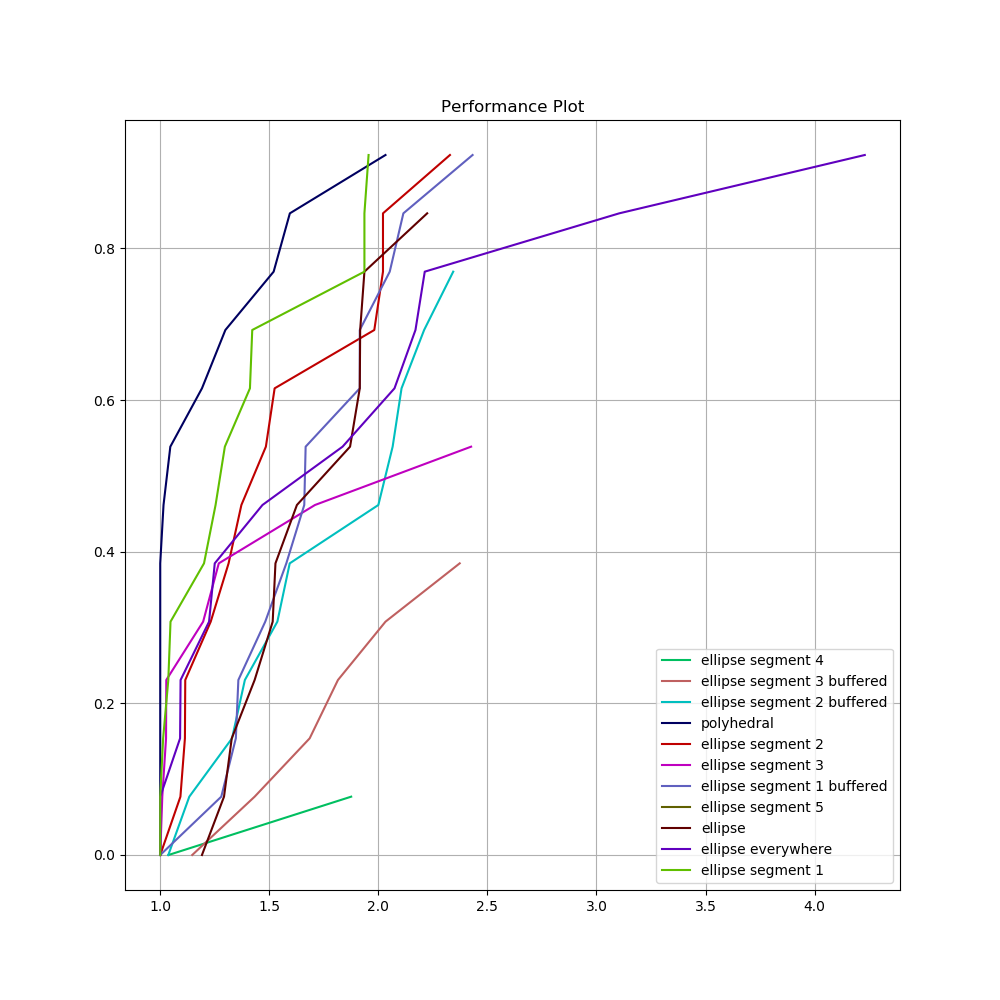
\includegraphics[scale=0.4]{images/performance_profile_plot.png}
    \caption{
    	\emph{Short:} A performance profile comparing different variants of the algorithm for linear constraints.
    	\emph{Long:} A performance profile comparing different variants of the algorithm for linear constraints.
    	We see that the polyhedral algorithm is both efficient and robust.
    }
    \label{performance_profile}
\end{figure}



The line segment search with 5 segments does not solve many problems, this is because several of the problems have dimension less than $5$, so that it was not even ran on these.
Notice that the polyhedral search does very well.
We conjecture that this may not hold with modelled, nonlinear constraints.


\subsection{Summary}
We still experienced a problem with iterates coming too close to the boundary of the feasible region.
Another way of dealing with this is to shift the constraints closer to the current iterate.
Namely, we introduce a parameter $\upsilon$ to determine how far to scale the constraints.
Then, within the trust region subproblem, we add constraints of $Ax \le b\upsilon + (1-\upsilon) A \xk $.
Before doing this, the rows of $A$ are normalized.
This produces the buffered segment searches withing the results.

% \color{red}
% 
% \section{Figure out where goes}
% 
% From here on, we will assume that the iterates $\xk$ are chosen according to \cref{linearly_constrained_dfo}.
% This implies that each of the sample points used to construct $\mfk$ are output of \cref{model_improving_algorithm}.
% 
% Because \cref{lipschitz_gradient} and \cref{lipschitz_hessian} are satisfied, $f$ also satisfies \cref{introduction_3_1} and hence the assumptions for \cref{quadratic_errors}.
% Notice that because $\kappa_f$, $\kappa_g$, $\kappa_h$ only depend on $p$, $L_h$, and $\Lambda$, these values do not depend on the iteration $k$:
% using the same tolerance $\xi_{\text{min}}$ within \cref{model_improving_algorithm} implies a bound on $\Lambda$.
% , and therefore $\mfk$ satisfies the requirements for \cref{quadratic_errors}.
% is a fully quadratic model over $B_{\infty}(\xk, \dk)$.
% \color{black}



\chapter{Nonlinear Constraints}\label{chap:convex}


\begin{boxedcomment}
Somewhere, I should talk about the same sample set being used for different orders of models.
\end{boxedcomment}

\label{infeasible_point_strategies}

The algorithm for general nonlinear constraints is complicated by the fact that we only have models for the constraint functions.
Errors in these models mean that we may attempt to evaluate a point that is not feasible in two ways:
\begin{itemize}
\item A sample point chosen by the geometry ensuring algorithm may be infeasible.
\item The trial point solving the trust region subproblem may be infeasible.
\end{itemize}



\begin{boxedcomment}
Consildate this discussion with the background.
\end{boxedcomment}

% What remains in throughout \cref{infeasible_point_strategies} is a discussion of various strategies
% for handling infeasible sample points.
To deal with these two forms of infeasible points, we have developed several strategies that make use of three separate trust regions.
These trust regions are a box-shaped outer trust region $\outertrk$,  an ellipsoidal inner trust-region $\sampletrk$ from which the sample points are chosen, 
and a search trust-region, $\searchtrk$, which constrains the search for the next iterate.

Note that the outer trust region may include infeasible points.
To ensure feasibility of all sample points, we construct an inner trust region  $ \sampletrk $  satisfying 
$\sampletrk \subset \outertrk \cap \feasiblek$.
Since $\feasiblek$ is only an approximation of $\feasible$,  we place additional restrictions on $\sampletrk$
to ensure that it is entirely contained within the feasible region $\feasible$.
These restrictions will be described in \cref{ellipsoid_requirements}, 
and we show that these restrictions ensure $\sampletrk \subset \feasible$ in \cref{ellipsoid_is_feasible} and \cref{searchtrk_is_feasible}.

%\cref{ellipsoid_is_feasible}

% However, we do not want to limit the search for a new iterate to the same trust region we use to construct the model.
The third trust region $\searchtrk$ is the search trust region, which could either be $\sampletrk$ itself, 
or a larger region satisfying $ \sampletrk \subset \searchtrk \subset \outertrk \cap \feasible$.
The search trust region is used in defining the trust region subproblem.

% \replace{
% Within our algorithm, if $ \outertrk \subseteq \feasible$ we can set $ \sampletrk $ to be a sphere of radius $\dk$.
% This saves the computation of $ \sampletrk $ when it is not needed, as there are no nearby constraints.}{}  \sbnote{I don't think this needs to be said here}

% In the last paper, we showed convergence of our algorithm for linear constraints.
% We follow the same pattern as in that paper, but we must deal with some problems introduced by general convex constraints.
% To avoid evaluating infeasible points with general convex constraints, we construct models of the constraints in addition to the objective.


What remains in \cref{infeasible_point_strategies} is devoted to search strategies for ensuring feasible sample points:
\cref{possible_ellipsoids} and \cref{handling_linear_constraints_within_ellipsoid_programs} could be considered background, while the others discuss algorithms.
The version we call the ``conservative ellipsoid'' is lengthier and discussed within \cref{constructing_and_analysizing_conservative_ellipsoid}.
Within \cref{convex_model_reduction} we examine two strategies for handling infeasible trial points.
Finally, in \cref{the_algroithm_section}, we state the convergent algorithm, which is based on the strategies found in 
\cref{constructing_and_analysizing_conservative_ellipsoid} and \cref{decreasing_the_trust_region_for_infeasible_trial}.



% We will show feasibility and convergence of the algorithm assuming certain of these 


% Although an approach for avoiding one of these two function evaluations can work for the other in thoery, we stick to one simplified version.

% \subsection{Implemented Ideas not used in this paper}
% 
% 
% \subsubsection{Using higher order models}
% I have implemented an algorithm that uses higher order models to approximate the constraints.
% 
% In this algorithm, we add additional degrees of freedom to the constraints to cut off points that have been evaluated and are infeasible.
% The models are forced to be a given negative value at these points.
% 
% One question for this method is how many constraints to model.
% 
% 
% I implemented Kriging, as this can use as many points as are available.
% However, this requires using some artificial value of the constraints at infeasible points.


\section{Constructing the Sample Region}
\label{possible_ellipsoids}

We ensure that sample points are feasible by constructing an inner trust region $\sampletrk$ that we show is feasible for small enough $\dk$.
\begin{boxedcomment}
Steve wants me to delete most of this...
\end{boxedcomment}
This means that if $\sampletrk$ includes infeasible points-and we attempt to evaluate at an infeasible point- we can reduced the trust region radius.
Of course, the method of constructing this ellipsoid impacts the algorithm's efficiency because constructing a $\sampletrk$ too small means a poor sample set,
while using a $\sampletrk$ too large implies reducing the trust region quickly so that only small steps can be made towards a critical point.

There is a well known algorithm for constructing poised sets over spheres, and this algorithm can be easily generalized to an ellipsoid.
Therefore, we construct an ellipsoidal inner trust region to avoid the constraints.


\subsection{Buffering Cones}
\label{ellipsoid_requirements}
% We construct a set of requirements $\sampletrk$ must satisfy.
During iteration $k$, let $\sampletrk$ be defined by a $n\times n$ symmetric, positive definite matrix $\qk$, center $\ck \in \Rn$, and radius $\delta_{k} > 0$:
\begin{align}
\sampletrk = \left \{x \in \Rn \bigg | \left(x - \ck\right)^T \qk\left(x - \ck\right) \le \frac 1 2 \sdk^2 \right \}. \label{define_sampletrk}
\end{align}
To ensure this ellipsoid is feasible, we construct cones that buffer the ellipsoid from the constraint boundaries.
These cones have a vertex between the current iterate and the nearest point along the linearization of the constraints, and open towards the current iterate.
We define these cones within this section.

The first step is to identify the set of constraints that are nearly active relative to the size of the current trust region.
Let $\zik$ denote the projection of the current iterate $\xk$ onto the hyperplane defined by the $i$-th constraint model.
% Specifically, for each $i$ with either $\left\|\gmcik\right\| \ne 0$ or $c_i\left(\xk\right) = 0$, define
Specifically, define

% vector of infinities
\begin{align}
\label{define_z}
\zik =
\begin{cases}
\xk &  c_i\left(\xk\right) = 0 \\
\xk - \frac{c_i\left(\xk\right)}{\left\|\gmcik\right\|^2} \gmcik & c_i\left(\xk\right) \ne 0 \quad \textrm{and} \quad \left\|\gmcik\right\| \ne 0 \\
\mathbf{\infty} & c_i\left(\xk\right) \ne 0 \quad \textrm{and} \quad \left\|\gmcik\right\| = 0 \\
\end{cases}
\end{align}
\begin{boxedcomment}
Note that $m^{(k)}_{c_i}\left(\xk\right) = c_i\left(\xk\right)$.
\end{boxedcomment}
% Note that this definition is consistent when both $c_i\left(\xk\right) = 0$ and $\left\|\gmcik\right\| \ne 0$.
If $\zik$ lies sufficiently near the outer trust region, we say that the $i$-th constraint is \emph{nearly active}.
Specifically, the set of nearly active constraints is defined by
\begin{align}
\activeconstraintsk = \left\{i \in [m] \bigg| \zik \in B_{\infty}\left(\xk, (1+\zikthresh)\dk\right)\right\}, \label{define_activeconstraints}
\end{align}
where $\zikthresh$ is a user defined parameter that must satisfy the following identity involving $\omegainc$ (which is defined by \cref{define_the_omegas}):
\begin{align}
(2 + \omegainc)\sqrt{n} < \zikthresh. \label{define_zikthresh}
\end{align}
For each nearly active constraint, we define a buffering cone with user defined parameters
\begin{align}
\alpha, \beta, p_{\alpha}, p_{\beta} \in (0, 1). \label{define_abpab}
\end{align}
The vertex $\wik$ of this cone is located along the line segment connecting $\xk$ to $\zik$:
\begin{align}
\wik = \xk + \left(1 - \alpha\dk^{p_{\alpha}}\right)\left(\zik - \xk\right) \forall i \in \activeconstraintsk. \label{define_w}
\end{align}
The cone for constraint $i$ is then defined by
\begin{align}
\fik = \left\{x \in \Rn | x = \wik + t s,t > 0, \|s\| = 1, -s^T\hgik \ge \beta \dk^{p_{\beta}} \right\}. \label{define_fik}
\end{align}
This cone is illustrated in \cref{explanation_2}.
\begin{figure}[ht]
    \centering
    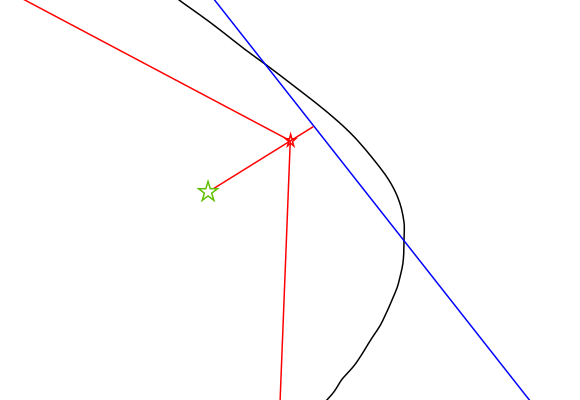
\includegraphics[width=150px]{images/explanation_2.png}
    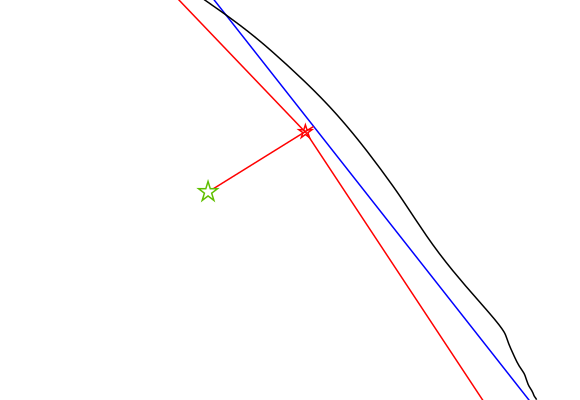
\includegraphics[width=150px]{images/explanation_3.png}
    \caption[An example of a buffering cone.]{
    	As the trust region goes to zero the buffering cone better approximates the linearization of the constraint and becomes locally feasible.
    	The current iterate is the green star;
    	the true constraint is black;
    	the vertex, $\wik$, is the red star;
    	the linearization of the constraint boundary is blue;
    	the cone buffering cone $\fik$ is in red.
	}
    \label{explanation_2}
\end{figure}
The intersection of these cones is the set
\begin{align}
\capcones = \{x\in\Rn | \; x \in \fik \quad \forall i \in \activeconstraintsk \} \label{define_capcones}
\end{align}
which is depicted in \cref{completed_2}.
In \cref{cone_and_tr_are_feasible}, we show that for sufficiently small $\dk$, $\capcones \cap \outertrkpo \subseteq \feasible$.
Therefore, to obtain feasible sample points, we require that 
\begin{align*}
\sampletrkpo \subset \capcones \cap \outertrkpo.
\end{align*}


\begin{figure}[ht]
    \centering
    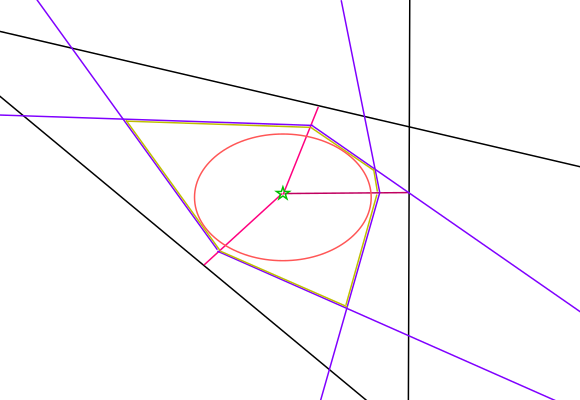
\includegraphics[width=150px]{images/completed_2.png}
    \caption
    	[An example ellipsoidal, buffered sample region.]{
    	After constructing 
    	the linearization of the constraints in black;
    	the buffering cones in blue;
    	the trusted region $\capcones$ in yellow;
    	we seek to find an ellipsoid within $\capcones$ such as the one in red/pink.
	}
    \label{completed_2}
\end{figure}


\subsection{Linear Constraints}
\label{handling_linear_constraints_within_ellipsoid_programs}

Throughout discussing strategies for constructing an ellipsoid within the buffering cones, we must also require that the ellipsoid is contained within the trust region.
Because our trust region is $\tr$, we can satisfy the trust region constraints by including linear constraints of the form $\xk_i - \dk \le x_i \le \xk_i + \dk$.
As done in the linear paper, using the work of \cite{Khachiyan1993}, we handle the general constraints $Ax \le b$ for some $m\times n$ matrix $A$ and $b \in \Rm$.
That is, given a polyhedron $P = \{ x \in \Rn\; | \;  Ax \le b \}$ defined by an $m \times n$ matrix $A$, and $b \in \Rm$,
we wish to find the maximum-volume ellipsoid $E \subset P$ centered at a point $\mu \in P$.

Let $\bar{b} = b - A\mu$ and $d = x - \mu$ so that the polyhedron becomes
\begin{align*}
P = \left\{ \mu + d \in \Rn \; \bigg | \;  Ad \le \bar{b} \right\}
\end{align*}
Then, the ellipsoid can then be centered at zero, and defined by a symmetric positive definite matrix $Q \succ 0$:
\begin{align*}
E =\left \{ d \in \Rn \; \bigg | \; \frac 1 2 d^T Q d \le 1 \right\}.
\end{align*}
Our goal is to determine $Q$ to maximize the volume of $E$ such that $\mu + E \subset P$.
Define the auxiliary function $f(d) = \frac 1 2 d^T Q d$ so that $E = \{ d \in \Rn\; | \; f(d) \le 1 \}$.

% Because $Q$ is positive definite, $f$ has a unique minimum on each hyper-plane $A_i d = b_i$.
% Let this minimum be $d^{(i)} = \argmin_{A_id =\bar{b}_i} f(d)$ for $i \in [m]$.
% By the first order optimality conditions, there exists a $\lambda \in \Rm$ such that
% \begin{align*}
% \gradf(d^{(i)}) = Q d^{(i)} = \lambda_i A_i 
% \Longrightarrow d^{(i)} = \lambda_i Q^{-1}A_i \quad \forall i \in [m]
% \end{align*}
% We also know that
% \begin{align*}
% A_i^T d^{(i)} = \bar{b_i} \Longrightarrow
% A_i^T \lambda_i Q^{-1}A_i = \bar{b_i} \Longrightarrow
% \lambda_i = \frac {\bar{b_i}}{A_i^T  Q^{-1}A_i}
% \end{align*}
% so that
% \begin{align*}
% d^{(i)} = \lambda_i Q^{-1}A_i = \frac {\bar{b_i}}{A_i^T  Q^{-1}A_i}  Q^{-1}A_i \quad \forall i \in [m].
% \end{align*}
% 
% Because $E \subset P$, we also know that $f(d^{(i)}) \ge 1$ for each $i$. Thus,
% \begin{align*}
% \frac 1 2 (d^{(i)})^{T} Q d^{(i)} \ge 1 \\
% \Longrightarrow \frac 1 2 \bigg(\frac {\bar{b}_i}{A_i^T  Q^{-1}A_i}  Q^{-1}A_i\bigg)^{T} Q \frac {\bar{b}_i}{A_i^T  Q^{-1}A_i}  Q^{-1}A_i \ge 1 \\
% \Longrightarrow \frac 1 2 \frac {1}{A_i^T  Q^{-1}A_i}  \bar{b_i} A_i^T Q^{-1} Q \frac {\bar{b_i}}{A_i^T  Q^{-1}A_i}  Q^{-1}A_i \ge 1 \\
% \Longrightarrow \frac 1 2 \frac {1}{A_i^T  Q^{-1}A_i}  \frac {\bar{b_i}^2}{A_i^T  Q^{-1}A_i}  A_i^T Q^{-1}A_i \ge 1 \\
% \Longrightarrow \frac 1 2  \frac {\bar{b_i}^2}{A_i^T  Q^{-1}A_i} \ge 1 \\
% \Longrightarrow \frac 1 2 \bar{b_i}^2\ge A_i^T  Q^{-1}A_i \\
% \Longrightarrow A_i^T  Q^{-1}A_i \le \frac 1 2 \bar{b_i}^2.
% \end{align*}

As shown in \cref{ellipse_optimization} these constraints can be simplified to requiring
\begin{align*}
A_i^T  Q^{-1}A_i \le \frac 1 2 \bar{b_i}^2 \forall i \in [m].
\end{align*}

For the trust region, this is can be written as
\begin{align*}
\tr = \left\{ x \in \Rn | \atr x\le \btr\left(\xk, \dk\right) \right\}
\end{align*}
where
\begin{align}
\atr = \begin{pmatrix}
 1 &  0 & 0      & \ldots &  0 \\
-1 &  0 & 0      & \ldots &  0 \\
 0 &  1 & 0      & \ldots &  0 \\
 0 & -1 & 0      & \ldots &  0 \\
   &    & \vdots &        &    \\
 0 &  0 &      0 & \ldots &  1 \\
 0 &  0 &      0 & \ldots & -1 \\
\end{pmatrix} \quad \textrm{and} \quad
\btr\left(\xk, \dk\right) = \atr \xk + \dk. \label{define_atr}
\end{align}
In row form, this is
\begin{align*}
e_i ^T x \le e_i^T\xk + \dk, \quad \textrm{and} \quad
-e_i ^T x \le -e_i^T\xk + \dk \quad \forall i \in [n],
\end{align*}
to ensure $\unshiftedellipsoid \subseteq \tr$, we must only constrain the diagonal elements of the inverse of $\qk$:
\begin{align}
e_i^T\left(\frac{\qk}{\frac 1 2 \sdk^2}\right)^{-1} e_i \le \left[e_i^T\left(\xk - \ck\right) \pm \dk \right]^2 \quad \forall i \in [n].
\label{ellipsoids_trust_region_constraints}
\end{align}



\subsection{Ideal Solution}
\label{ideal_ellipsoid_in_polyhedron}

One strategy would be to create the largest possible ellipsoid that is contained within each of the cones $\fik$ defined in \cref{define_fik}.
Although this sounds appealing, we were only able to formulate this problem as a multilevel optimization problem.
However, it is possible to formulate the problem of checking whether an ellipsoid is contained within any particular cone.
This admits a search over possible ellipsoids, with an algorithmic check that is efficient.
We discuss this here.
Throughout, we will assume that the constraints found in \cref{ellipsoids_trust_region_constraints} are included, 
to ensure the ellipsoid is within the outer trust region $\outertrk$.
% \begin{align*}
% \max_{\qk, \ck, \sk} \det\left(\qk^{-1}\right) \\
% \end{align*}

Notice that because the cone for each constraint opens toward the current iterate,
and each cone uses the same threshold $\beta \dk^{p_\beta}$ for feasible directions from the vertex,
the cones can be uniquely defined by their vertices.
This means that for an iteration $k$, after a change of variables
\begin{align}
x \gets x - \xk \\
v^{(i)}  \gets \wik - \xk \\
\beta \gets \beta \dk^{p_{\beta}},
\end{align}
each cone in \cref{define_fik} is equivalent to
\begin{align*}
A_i = \fik - \xk = \left\{x\in\Rn\bigg|\;-\frac{(x - v^{(i)})^T}{\|x - v^{(i)}\|} \frac{v^{(i)}}{\|v^{(i)}\|} \ge \beta \right\}.
\end{align*}
Now, the ellipsoid $\sampletrk$ is contained in each a cone $A_i$ if and only if the \emph{perspective projection} from $v^{(i)}$ of the ellipsoid onto the hyper-plane 
\begin{align*}
H_i = \left\{x \in \Rn \bigg|\left(v^{(i)}\right)^Tx = 0\right\}
\end{align*}
is contained in the projection of the cone.
The perspective projection onto $v^{(i)}$ is the shape drawn onto a hyperplane as if a viewer were positioned at $v^{(i)}$.
That is, imagine a viewer is positioned at $v^{(j)}$, and viewing the ellipsoid as in \cref{perspective_projection_depiction}.
They create a line from $v^{(j)}$ to the hyperplane by looking past the outer edge of the ellipsoid onto the hyper plane.
If they were to trace all possible rays through the boundary of the ellipsoid onto the hyperplane, 
these rays intersect the hyperplane on the ellipsoid's perspective projection.


\begin{figure}[ht]
    \centering
    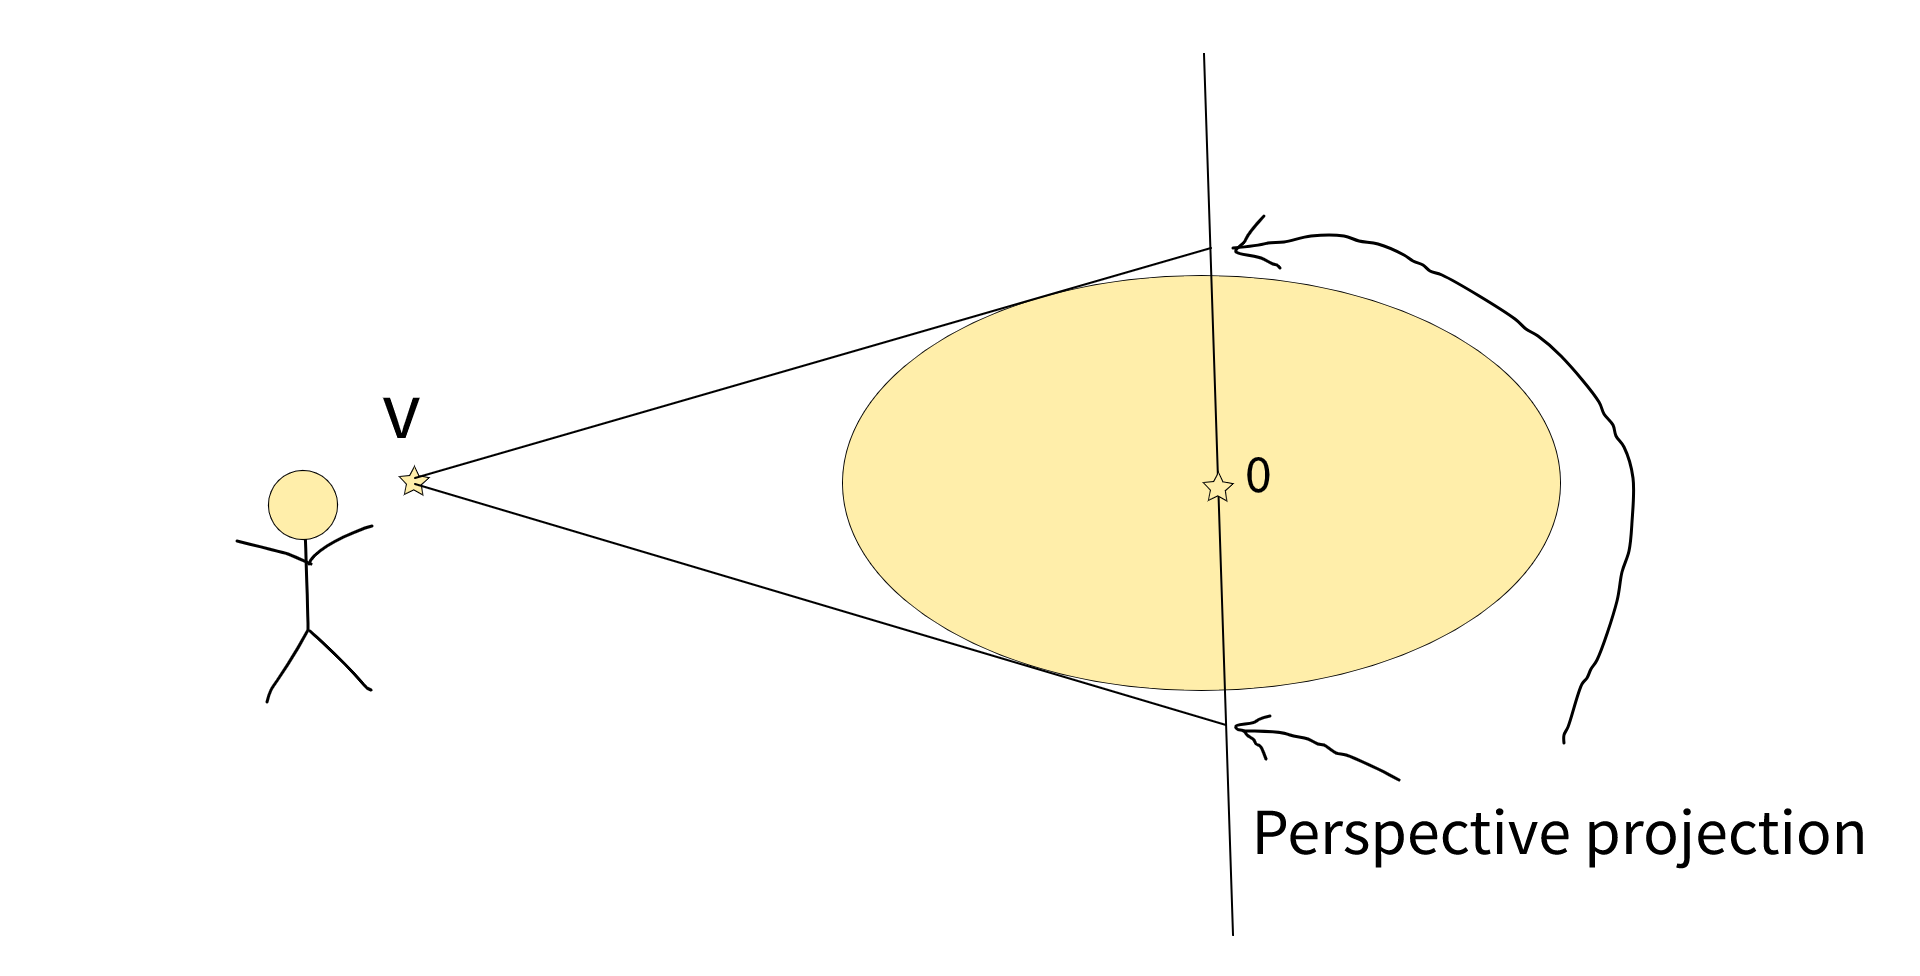
\includegraphics[width=300px]{images/perspective_projection.png}
    \caption[A depiction of the perspective projection]{
    		The perspective projection is the intersection of the plane and directions from $V$ through the boundary of the ellipsoid.
	}
    \label{perspective_projection_depiction}
\end{figure}

First, we compute the projection of the cone, which is simply its intersection with the hyperplane:
\begin{align*}
H_i \cap A_i 
= \left\{x \in \Rn \bigg| \left(v^{(i)}\right)^Tx = 0, -\frac{\left(x - v^{(i)}\right)^T}{\|x - v^{(i)}\|}\frac{v^{(i)}}{\|v^{(i)}\|}\ge \beta \right\} \\
= \left\{x \in \Rn \bigg| \left(v^{(i)}\right)^Tx = 0, \|v^{(i)}\|\ge \beta\|x - v^{(i)}\| \right\} \\
= \left\{x \in \Rn \bigg| \left(v^{(i)}\right)^Tx = 0, \|x - v^{(i)}\|^2 \le \frac 1 {\beta^2}\|v^{(i)}\|^2 \right\} \\
= \left\{x \in \Rn \bigg| \left(v^{(i)}\right)^Tx = 0, \|x\|^2 \le \left(\frac 1 {\beta^2} - 1\right)\|v^{(i)}\|^2 \right\}.
\end{align*}

Then, we can compute the perspective projection of the ellipsoid, in a fashion similar to \cite{eberly_2013}.
Consider the point $x = v^{(i)} + td$ for some unit direction $d$ and distance $t$ from $v^{(i)}$.
If $x$ is on the boundary of the ellipsoid, then:
\begin{align*}
0 = (v^{(i)} + t d - \ck )^T \qk  (v^{(i)} + t d - \ck ) - 1\\
= (v^{(i)} + t d - \ck )^T \qk  v^{(i)} + t (v^{(i)} + t d - \ck )^T \qk d \\ - (v^{(i)} + t d - \ck )^T \qk \ck - 1\\
= \left(v^{(i)}\right)^T \qk  v^{(i)} + t d^T \qk  v^{(i)} - \ck ^T \qk  v^{(i)} + t \left(v^{(i)}\right)^T \qk  d \\ + t^2 d^T \qk  d - t \ck ^T \qk  d - \left(v^{(i)}\right)^T \qk  \ck  - t d^T \qk  \ck + \ck ^T \qk \ck - 1\\
= \left(d^T\qk d
\right) t^2 + \left(
d^T \qk  v^{(i)} +  \left(v^{(i)}\right)^T \qk  d - \ck ^T \qk  d - d^T \qk  \ck 
\right) t \\ +  \left(
\left(v^{(i)}\right)^T \qk  v^{(i)} - \ck ^T \qk  v^{(i)} - \left(v^{(i)}\right)^T \qk  \ck   + \ck ^T \qk  \ck  - 1
\right) \\
= \left[d^T\qk d
\right] t^2 + 2\left[
\left(v^{(i)}\right)^T \qk  d - \ck ^T\qk d
\right] t + \\ \left[
\left(v^{(i)}\right)^T \qk  v^{(i)} + \ck ^T \qk  \ck  - 2 \ck ^T \qk  v^{(i)} - 1
\right]
\end{align*}

There are either $0$, $1$, or $2$ values of $t$ for which this equation will have solutions.
The directions from $v^{(i)}$ with exactly $1$ intersection with the ellipsoid are those whose projection will be on the boundary of the perspective projection of the ellipsoid.
The discriminant for these is $0$.
If we let
\begin{align*}
M_i = 
\qk (v^{(i)} - \ck )\left[\qk (v^{(i)} - \ck )\right]^T \\
- \qk  \left(\left(v^{(i)}\right)^T \qk  v^{(i)} + \ck ^T \qk  \ck  - 2 \ck ^T \qk  v^{(i)} - 1\right),
\end{align*}
we find that that these directions satisfy
\begin{align*}
4\left(\left(v^{(i)}\right)^T \qk  d - \ck ^T\qk d\right)^2 \\
- 4 \left(d^T\qk d\right) \left(\left(v^{(i)}\right)^T \qk  v^{(i)} + \ck ^T \qk  \ck  - 2 \ck ^T \qk  v^{(i)} - 1\right) \\
= d^TM_id = 0.
\end{align*}

% This used to be a line, but it didn't fit...
% d^T\left[
% \left(\qk (v^{(i)} - \ck )\right)\left(\qk (v^{(i)} - \ck )\right)^T
% - \qk  \left(\left(v^{(i)}\right)^T \qk  v^{(i)} + \ck ^T \qk  \ck  - 2 \ck ^T \qk  v^{(i)} - 1\right)\right]d = 0 \\

Next, let
\begin{align*}
t = -\frac {\left(v^{(i)}\right)^T v^{(i)}}{\left(v^{(i)}\right)^T d } \Longrightarrow
0 = \left(v^{(i)}\right)^T v^{(i)} + t {v^{(i)}}^T d \Longrightarrow
0 = \left(v^{(i)}\right)^T \left(v^{(i)} + t d\right)
\end{align*}
so that $x \in H_i$.
We already know that
\begin{align*}
x = v^{(i)} + t d \Longrightarrow
d = \frac 1 t \left(x - v^{(i)}\right)
\Longrightarrow d^TM_id = \frac 1 {t^2} \left(x - v^{(i)}\right)^TM_i\left(x - v^{(i)}\right) = 0
\end{align*}
so the perspective projection of the boundary of the ellipsoid on the hyper-plane $H_i$ is described by
\begin{align*}
\{x \in \Rn | {v^{(i)}}^Tx = 0, \left(x - v^{(i)}\right)^TM_i\left(x - v^{(i)}\right) = 0\}
\end{align*}

Thus, the ellipsoid is contained in cone $A_i$ if and only if
\begin{align*}
\{x \in \Rn | {v^{(i)}}^Tx = 0, \left(x - v^{(i)}\right)^TM\left(x - v^{(i)}\right) = 0\} \\
\subseteq \{x \in \Rn | {v^{(i)}}^Tx = 0, \|x - v^{(i)}\|^2 \le \frac 1 {\beta_i^2}\|v^{(i)}\|^2 \} \\
= \{x \in \Rn | {v^{(i)}}^Tx = 0, \|x\|^2 \le \left(\frac 1 {\beta_i^2} - 1\right)\|v^{(i)}\|^2 \}.
\end{align*}

For each $i \in [m]$, define
\begin{align*}
\hat v^{(i)} = \frac{v^{(i)}}{\|v^{(i)}\|} \\
R^i = 2\frac{(\hat v^{(i)} + e_1)(\hat v^{(i)} + e_1)^T}{(\hat v^{(i)} + e_1)^T(\hat v^{(i)} + e_1)} - I
\end{align*}
so that
\begin{align*}
& {R^i}v^{(i)} = \|v^{(i)}\|e_1 & {R^i}^T{R^i} = I & \quad \det({R^i}) \in \{-1, 1\}
\end{align*}
and let $W_i$, $y$, $w_{1,1}$, $w_1$ be defined so that
\begin{align*}
& M_i = {R^i}^T M_i' {R^i} = {R^i}^T\left( \begin{array}{cc}
{w_{1,1}^i} & {w_1^i} \\
{w_1^i}^T	& {W_i}  \\
\end{array} \right){R^i} &
{R^i}x = \left(\begin{array}{c}
0 \\
y
\end{array}\right)
\end{align*}
for all $x$ with $x^Tv = 0$.
Then
\begin{align*}
0 = \left(x - {v^{(i)}}\right)^TM_i\left(x - {v^{(i)}}\right) \\
= x^TM_ix - 2x^TM_i{v^{(i)}} + {v^{(i)}}^TM_i{v^{(i)}} \\
= x^T{R^i}^TM_i'{R^i}x - 2x^T{R^i}^TM_i'{R^i}{v^{(i)}} + {v^{(i)}}^T{R^i}^TM_i'{R^i}{v^{(i)}} \\
= y^T{W_i}y - 2\|v^{(i)}\|y^Tw_1^i + {w_{1,1}^i}\|v^{(i)}\|^2 \\
\Longleftrightarrow y^T{W_i}y - 2\|v^{(i)}\|y^T{W_i}{W_i}^{-1}{w_1^i} + \|v^{(i)}\|^2{{w_1^i}}^T{W_i}^{-1}{W_i}{W_i}^{-1}{w_1^i} \\
= - \|v^{(i)}\|^2{w_{1,1}^i} + \|v^{(i)}\|^2{{w_1^i}}^T{W_i}^{-1}{W_i}{W_i}^{-1}{w_1^i} \\
\Longleftrightarrow \left(y - \|v^{(i)}\|{W_i}^{-1}{w_1^i}\right)^T{W_i}\left(y - \|v^{(i)}\|{W_i}^{-1}{w_1^i}\right) \\
= - \|v^{(i)}\|^2{w_{1,1}^i} + \|v^{(i)}\|^2{{{w_1^i}}}^T{W_i}^{-1}{{w_1^i}} \\
\end{align*}

Thus, to find the maximum norm $x$ with $\left(v^{(i)}\right)^Tx = 0$, we wish to compute:
\begin{align*}
\max_{y} & \quad \|y\|^2  \\
 & \left(y - \|v^{(i)}\|{W_i}^{-1}{w_1^i}\right)^T{W_i}\left(y - \|v^{(i)}\|{W_i}^{-1}{w_1^i}\right) = - \|v^{(i)}\|^2{w_{1,1}^i} + \|v^{(i)}\|^2{{w_1^i}}^T{W_i}^{-1}{w_1^i}
\end{align*}

After a change of variables
\begin{align*}
w_c \gets \|v^{(i)}\|{W_i}^{-1}w_1^i \\
w_r \gets  - \|v^{(i)}\|^2{w_{1,1}^i} + \|v^{(i)}\|{{w_1^i}}^Tw_c \\
s \gets y - w_c
\end{align*}
this becomes:

\begin{align}
\label{cone_feasibility_check}
\begin{array}{ccc}
\max_{y} & \quad \|s - \left(-w_c\right)\|^2  \\
 & s^T\left(\frac {W_i}{w_r}\right)s = 1
 \end{array}
\end{align}

% This is the well known optimization problem of projecting a point onto the surface of an ellipsoid.
To our knowledge, no explicit solution exists, 
which leaves us to believe that there is no explicit formulation of finding the maximum volume ellipsoid contained within the intersection of these cones.
However, there is an efficient, binary-search algorithm to solve this.
% \cite{projecttoellipsoid}.


Namely, given 
$p \in \Rn$ and a matrix $Q$,
we can consider how to compute point furthest from $p$ that is also in the set $\left\{x \in \Rn \bigg | x^TQx = 1 \right\}$:
\begin{align}
\begin{array}{ccc}
x^{\star} = &\argmax_{x \in \Rn} & \|x - p\|^2 \\
& \textrm{s.t.} & x^TQx = 1.
\end{array} \label{antiprojection_problem}
\end{align}
% If $p^TQp \le 1$, then clearly $x^{\star} = p$.
The first order optimality conditions imply the existence of a $\lambda \in \reals$ such that
% x^{\star} - p = \lambda Qx^{\star} \Longleftrightarrow \left(Q - \frac 1 {\lambda} I\right)x^{\star} = -\frac 1 {\lambda}p \\
\begin{align*}
x^{\star} - p = \lambda Qx^{\star} %\Longleftrightarrow \left(\lambda Q - I\right)x^{\star} = -p
\Longleftrightarrow x^{\star} = -\left(\lambda Q - I\right)^{-1}p
\end{align*}
provided the inverse exists.
Using $\left(x^{\star}\right)^TQx^{\star} = 1$, the problem reduces to finding zeros of the function $f : \reals_+ \to \reals$ defined by
\begin{align*}
f(\lambda) = p^T\left(\lambda Q - I\right)^{-1}Q\left(\lambda Q - I\right)^{-1}p - 1.
\end{align*}
Notice 
\begin{itemize}
\item $f(0) = p^TQp - 1 > 0$
\item $\lim_{\lambda \to \frac 1 {\lambda_i}} f(\lambda) = \infty$ for any eigenvalue $\lambda_i$
\item the presence of $\lambda$ within inverse expressions suggests $\lim_{\lambda \to \pm \infty}f(\lambda) = -1$
\end{itemize}
A binary search on $\lambda$ can find the zeros of $f$.


\begin{figure}[ht]
    \centering
    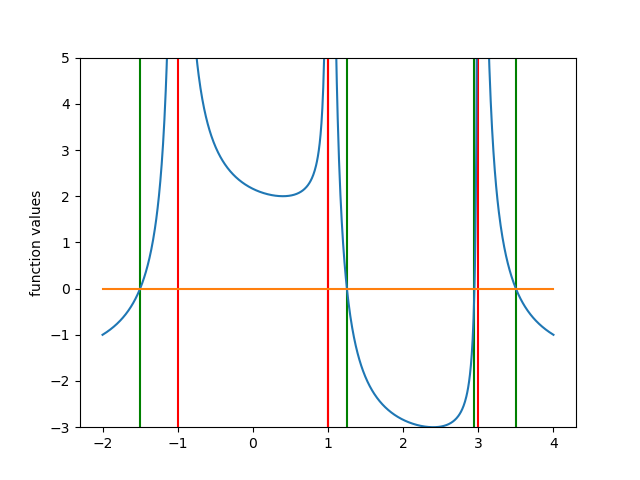
\includegraphics[width=300px]{images/antiprojection.png}
    \caption[
    		An example plot of the one-dimensional function whose zeros provide the largest ellipsoid within the buffering cones.
		]{
    		By computing the zeros of this function, we find values of $\lambda$ for each critical point of \cref{antiprojection_problem}.
    		The function $f$ is in blue, and the eigenvalues of $Q$ are red vertical lines.
    		A binary seach can be used to find one zero (plotted as green vertical lines) to the left of the smallest eigenvalue and one to the right of the largest.
    		Between any two eigenvalues, we first find the minimum.
    		If the minimum is negative, we can then use a binary search to compute two more zeros.
	}
    \label{feasible_direction}
\end{figure}





% \subsubsection{Numerical Solution}
% 
% Although the algorithm presented in \cref{ideal_ellipsoid_in_polyhedron} yields a solution that cannot be solved explicitly, it is easy to check if an ellipsoid is feasible using \cref{cone_feasibility_check}.
% One very simple random-search algorithm can be used to show this.
% 
% \begin{boxedcomment}
% Dramatically simplify this algorithm...
% \end{boxedcomment}
% 
% \begin{algorithm}[H]
%     \caption{Search for feasible ellipsoid}
%     \label{numerical_ellipsoid_algorithm}
%     \begin{itemize}
%         \item[\textbf{Step 0}] \textbf{(Initialization)} \\
%                 Set $E_{max}$ to any feasible ellipsoid, 
%                 an initial sample variance $\sigma^2$, 
%                 a threshold $M$ of iterations per sample variance, 
%                 a decrease ratio $\gamma \in (0, 1)$, 
%                 a variance tolerance $\delta_{\sigma} > 0$
%         
%         \item[\textbf{Step 1}] \textbf{(Random Perturbation)} \\
%             Evaluate the next iterate \begin{itemize}
%                 \item[] Sample a rotation matrix $R$ with variance $\sigma^2$, $\qk \gets R \qk$
%                 \item[] Sample a positive diagonal matrix $D$ with variance $\sigma^2$, $\qk \gets D \qk$
%                 \item[] Sample a translation $c$ bounded by with variance $\sigma^2$, $\ck \gets c + \ck$
%             \end{itemize}
%         
%         \item[\textbf{Step 2}] \textbf{(Check Feasibility)} \\
%             Run feasibility check \cref{cone_feasibility_check} for each constraint.
%             If the new ellipsoid is feasible and larger than $E_{max}$, then 
%             	set $E_{max}$ to this ellipsoid,
%             	set counter $j \gets 0$, and
%             	go to Step 1
%         
%         \item[\textbf{Step 3}] \textbf{(Decrease Sample Variance)} \\
%             If the counter $j \ge M$, then
% 	    	decrease $\sigma^2 \gets \gamma \sigma^2$,
% 	    	set the counter $j\gets 0$, and
% 	    	go to Step 1
%             
%         \item[\textbf{Step 4}] \textbf{(Check for Convergence)} \\
% 	    If $\sigma^2 < \delta_{\sigma}$ \textbf{Return} $E_{max}$.
% 	    Otherwise, 
%         		set counter $j \gets j + 1$, and
%         		go to Step 1
%     \end{itemize}
% \end{algorithm}
% 
% Although not efficient, this can be used to find a large ellipsoid within the buffering cones.


\subsection{Spherical Solution}

One simplification that allows an explicit formulation is to restrict the ellipsoid to be a sphere.
Although this may produce an ellipsoid with less volume, it may be used as a hot start while searching over all ellipsoids.

To compute the maximum volume sphere, we can maximize the minimum distance from the center of the sphere to any cone.
We once again perform a change of variables, this time subtracting of $\xk$ and rotating $v^{(i)}$ onto $e_1$.
This reduces the problem computing the projection of an arbitrary point $(t, y) \in \Rn$ and the second order cone: $\left\{ x \in \mathbb R^n | \quad x^Te_1 = \beta \|x\| \right\}$ for some $\beta \in \reals$.
We find
\begin{align*}
 \\
x^Te_1 = \beta \|x\| 
 \Longleftrightarrow t^2 = \beta^2 \|te_1  + x - t e_1\|^2 
  = \beta^2 \left(\|te_1\|^2  + \|x - t e_1\|^2\right) \\
= \beta^2 \left(t^2  + \|y\|^2 \right) 
 \Longleftrightarrow (1 - \beta^2)t^2 = \beta^2 \|y\|^2 
 \Longleftrightarrow \sqrt{\frac{1 - \beta^2}{ \beta^2}} t = \|y\|.
\end{align*}

%  \Longleftrightarrow t^2 = \beta^2 \left(\|te_1\|^2  + \|x - t e_1\|^2\right) \\

This means, that if we let $\beta' = \sqrt{\frac{1 - \beta^2}{\beta^2}}$, we have
\begin{align*}
\left\{ x \in \mathbb R^n | \quad x^Te_1 = \beta \|x\| \right\} = \left \{(s, x)\in \mathbb R^n | \quad\|x\| \le \beta' s \right\}.
\end{align*}

The projection gives the following optimization problem:
\begin{align*}
\min_{x \in \mathbb R^{n-1}, s \in \mathbb R} & \quad \frac 1 2 \|x - y\|^2 + \frac 1 2 (s - t)^2 \\
	\textrm{s.t.}		& \quad \frac 1 2 \|x\|^2 = \frac 1 2 {\beta'}^2 s^2,
\end{align*}
with Lagrangian:
\begin{align*}
l(x, s, \lambda) = \frac 1 2 \|x - y \|^2 + \frac 1 2 \left(s - t\right)^2 - \lambda \frac 1 2 \left(\|x\|^2 - {\beta'}^2 s^2\right).
\end{align*}

After taking the gradient of the Lagrangian, the first order optimality conditions imply that for some $\lambda \in \reals$:
\begin{align*}
x - y - \lambda x = 0, & \quad s - t + \lambda {\beta'}^2 s = 0 \\
x = \frac {y}{1 - \lambda}, & \quad s = \frac {t}{1 + \lambda {\beta'}^2 }.
\end{align*}

We can substitute this into the constraint to solve for $\lambda$:
\begin{align*}
\|x\| = {\beta'} s \\
\left\|\frac {y}{1 - \lambda}\right\| = {\beta'} \frac {t}{1 + \lambda {\beta'}^2 } \\
\left(1 + \lambda {\beta'}^2\right) \left\|y\right\| = {\beta'}  {t} \left|1 - \lambda\right|
\end{align*}

\begin{align*}
\left\|y\right\| + {\beta'}^2\left\|y\right\|\lambda = t {\beta'} - t {\beta'} \lambda          &   \quad
\left\|y\right\| + {\beta'}^2\left\|y\right\|\lambda = t {\beta'} \lambda - t {\beta'}					\\
\left\|y\right\|-t {\beta'} +\left( {\beta'}^2\left\|y\right\| + t {\beta'} \right)\lambda = 0  &		\\
\lambda = \frac{t {\beta'} - \|y\|}{{\beta'}^2\|y\| + t {\beta'}}                               &		
\end{align*}


Substituting $\lambda$ to find $x$ and $s$:
\begin{align*}
x = \frac {y}{1 - \lambda} 																		
= \frac {y}{1 - \frac{t{\beta'} - \|y\|}{{\beta'}^2\|y\| + t{\beta'}}} 									
= \frac {y\left({\beta'}^2\|y\| + t{\beta'}\right)}{{\beta'}^2\|y\| + t{\beta'} - t{\beta'} + \|y\|} 			
= \frac {{\beta'}^2 + \frac{t{\beta'}}{\|y\|}}{1 + {\beta'}^2}y 											
\end{align*}

\begin{align*}
s = \frac {t}{1 + \lambda{\beta'}^2 } 
= \frac {t}{1 +\frac{t{\beta'} - \|y\|}{{\beta'}^2\|y\| + t{\beta'}}{\beta'}^2 } 
= \frac {t\left({\beta'}^2\|y\| + t{\beta'}\right)}{{\beta'}^2\|y\| + t{\beta'} + \left(t{\beta'} - \|y\|\right){\beta'}^2 } 
= \frac {{\beta'}\|y\| + t}{1 + {\beta'}^2 } 
\end{align*}


Thus, the projected point is
\begin{align*}
\left(\frac{{\beta'} \|y\| + t}{1 + {\beta'} ^ 2}, \frac{{\beta'} ^ 2 + t \frac {{\beta'}}{\|y\|}}{1 + {\beta'} ^ 2}y\right)
\end{align*}
with squared distance
\begin{align*}
\left(\frac{{\beta'} \|y\| + t}{1 + {\beta'} ^ 2} - t\right)^2 + \left\|\frac{{\beta'} ^ 2 + t \frac {{\beta'}}{\|y\|}}{1 + {\beta'} ^ 2}y - y\right\|^2 \\
= \left(\frac{{\beta'} \|y\| + t}{1 + {\beta'} ^ 2} - \frac{t + t{\beta'} ^ 2}{1 + {\beta'} ^ 2}\right)^2 + \left(\frac{{\beta'} ^ 2 + t \frac {{\beta'}}{\|y\|}}{1 + {\beta'} ^ 2} - 1\right)^2\left\|y\right\|^2 \\
= \left(\frac{{\beta'} \|y\| - t{\beta'}^2}{1 + {\beta'} ^ 2}\right)^2 + \left(\frac{{\beta'} ^ 2 + t \frac {{\beta'}}{\|y\|} - 1 - {\beta'} ^ 2}{1 + {\beta'} ^ 2}\right)^2\left\|y\right\|^2 \\
= \left(\frac{{\beta'} \|y\| - t{\beta'}^2}{1 + {\beta'} ^ 2}\right)^2 + \left(\frac{t {\beta'} - \left\|y\right\|}{1 + {\beta'} ^ 2}\right)^2 \\
= \left(1 + {\beta'}^2\right)^{-2}\left[\left({\beta'}^2 \|y\|^2 - 2\beta' \|y\| t {\beta'}^2  + t^2 {\beta'}^4\right) + \left(t^2{\beta'}^2 - 2 t {\beta'} \|y\| + \|y\|^2\right) \right] \\
= \left(1 + {\beta'}^2\right)^{-2}\left[
\left(1 + {\beta'}^2\right)t^2{\beta'}^2 - 2t{\beta'}\left(1 + {\beta'}^2\right) \|y\| + \left(1 + {\beta'}^2\right)\|y\|^2
\right] \\
= \frac{\left(t \beta' - \|y\|\right)^2}{1 + {\beta'}^2}
\end{align*}

We summarize the previous statements here:
\begin{lemma}
Let $t \in \reals$, $y \in \mathbb R^{n-1}$, and $\beta' > 0$.
Then the point
\begin{align*}
z = \left(1 + {\beta'} ^ 2\right)^{-1} \left({\beta'} \|y\| + t, \left({\beta'} ^ 2 + t \frac {{\beta'}}{\|y\|}\right) y\right)
\end{align*}
satisfies
\begin{align*}
z = \argmin_{\left\|x\right\| \le \beta' s} \left\|x - y\right\|^2 + \left\|s - t\right\|^2 \\
\left\|z - (t, y)\right\|^2 = \left(1 + {\beta'}^2\right)^{-1}\left(t \beta' - \left\|y\right\| \right)^2.
\end{align*}
\end{lemma}

After a shift and rotation from the vertex point $\wik$ and going direction $-\wik$:

\begin{align*}
\hat w^{(i,k)} = \frac {\wik} {\|\wik\|} & \quad \forall i \in [m] \\
R^j = 2 \frac{(e_1 + \hat w^{(i,k)})(e_1 + \hat w^{(i,k)})^T}{(e_1 + \hat w^{(i,k)})^T(e_1 + \hat w^{(i,k)})} - I  & \quad \forall j \in [m],
\end{align*}
we have the following optimization problem:
\begin{align*}
\begin{array} {ccc}
\max_{r \ge 0, c, t^i}	& r & \\
					& t^i = R^j\left(\hat w^{(i,k)} - c\right) 									& \quad \forall i \in [m] \\
					& \beta^2 \left(\beta' e_1^T t^i - \left\|t^i - e_1^T t^j\right\|\right)^2 \ge r			& \quad \forall i \in [m] \\
					& \left(\left(c - w^j\right)^T\hat w^{(i,k)}\right)^2 \ge \beta^2 \|c - \wik\|^2		& \quad \forall i \in [m] \\
					& c \in \tr &
\end{array}
\end{align*}

% 
% \begin{boxedcomment}
% What did the following few lines do, again?
% \end{boxedcomment}
% 
% \begin{align*}
% \beta^2 \left(\beta' e_1^T t^j - \left\|t^j - e_1^T t^j\right\|\right)^2 \ge r \\
% \beta \left(\beta' e_1^T t^j - \left\|t^j - e_1^T t^j\right\|\right) \ge \sqrt{r} \\
% \beta \beta' e_1^T t^j - \beta \left\|t^j - e_1^T t^j\right\| \ge \sqrt{r} \\
% \beta' e_1^T t^j - \frac 1 {\beta} \sqrt{r} \ge \left\|t^j - e_1^T t^j\right\| \\
% \left( \beta' e_1^T t^j - \frac 1 {\beta} \sqrt{r} \right) ^ 2\ge \left\|t^j - e_1^T t^j\right\|^2 \\
% \end{align*}
% 
% 
% 
% 
% \begin{align*}
%  \left(\beta' e_1^T t^j - \left\|t^j - e_1^T t^j\right\|\right)^2 \ge \frac 1 {\beta^2} r \\
%  \left(\beta' e_1^T t^j\right)^2 - 2\beta' e_1^T t^j \left\|t^j - e_1^T t^j\right\| + \left\|t^j - e_1^T t^j\right\|^2 \ge \frac 1 {\beta^2} r \\
%  \left(\beta' e_1^T t^j\right)^2 - \frac 1 {\beta^2} r + \left\|t^j - e_1^T t^j\right\|^2 \ge 2\beta' e_1^T t^j \left\|t^j - e_1^T t^j\right\|\\
%  \left[\left(\beta' e_1^T t^j\right)^2 - \frac 1 {\beta^2} r + \left\|t^j - e_1^T t^j\right\|^2 \right] ^2\ge 4\left(\beta' e_1^T t^j\right)^2 \left\|t^j - e_1^T t^j\right\|^2\\
% \end{align*}
% 

Notice that this optimization problem is not convex.
Although more efficient formulations may exist, this leads us to believe that it may sometimes be difficult to even compute the maximum volume sphere within the buffering cones.

\subsection{Conservative Ellipsoid}
Throughout \cref{possible_ellipsoids} we have considered several inner trust regions.
However, we are not able to show that these formulations satisfy the requirements necessary for convergence.
% not been able to show that these satisfied the requirements stated in \cref{ellipsoids_notation_definitions}.
We were able to find an ellipsoid contained within each \cref{define_fik} that may, in general, be smaller than the largest possible ellipsoid.
Because we analyse this in more depth, we dedicate \cref{constructing_and_analysizing_conservative_ellipsoid} to this.

\section{Conservative Ellipsoid Derivation}
\label{constructing_and_analysizing_conservative_ellipsoid}

We state the ellipsoid requirements required for convergence in \cref{ellipsoids_notation_definitions}, and then show the conservative ellipsoid satisfies them.
Note the criteria in \cref{ellipsoids_notation_definitions} only summarize one of many possible sets of criteria sufficient for convergence.

\begin{definition}
\label[definition]{ellipsoids_notation_definitions}
For each $k \in \naturals$, suppose we are given $n\times n$, symmetric, positive-definite matrices $\qk$, vectors $\ck \in \Rn$, scalars $\sdk > 0$.
We have the following definitions.
\begin{itemize}
\item The sequence $(\qk, \ck, \sdk)$ is \emph{conditioned} if the condition numbers of $\qk$ are bounded for small enough $\dk$.
That is, there exists a $\sigmamax \ge 1$ and $\dacc > 0$ such that if $\dk \le \dacc$, then
\begin{align}
\condition \left(\qk\right) \le \sigmamax. \label{define_suitable_condition_numbers}
\end{align}
\item The tuple $(\qkpo, \ckpo, \sdkpo)$ is \emph{trusted} for $\xkpo, \dkpo$ if an ellipsoid defined by $\qkpo, \ckpo, \sdkpo$ lies within $ \capcones \cap \trkpo $.
That is,
\begin{align}
\unshiftedellipsoidkpo \subseteq \capcones \cap \trkpo  \label{define_suitable_in_tr}
\end{align}
where
\begin{align}
\unshiftedellipsoid = \left\{x \in \Rn | \left(x - \ck \right)^T \qk \left(x - \ck\right) \le \frac 1 2 {\sdk}^2 \right\} \label{define_unshifed_ellipsoid}
\end{align}
\item The tuple $(\qk, \ck, \sdk)$ is \emph{feasible} if an ellipsoid defined by $\qk, \ck, \sdk$ lies within the feasible region:
\begin{align}
\unshiftedellipsoid \subseteq \feasible.
\end{align}
where $\unshiftedellipsoid$ is defined by \cref{define_unshifed_ellipsoid}
\item The tuple $(\qk, \ck, \sdk)$ is \emph{adjacent} to $\xk$ if an ellipsoid defined by $\qk, \ck, \sdk$ is near to the current iterate:
\begin{align}
\xk \in \scaledunshiftedellipsoid \label{define_suitable_close_to_iterate}
\end{align}
where
\begin{align}
\scaledunshiftedellipsoid = \left\{x \in \Rn | \left(x - \ck\right)^T \qk \left(x - \ck\right) \le {\sdk}^2 \right\} \label{define_scaledunshiftedellipsoid}
\end{align}
\item The tuple $(\qk, \ck, \sdk)$ is \emph{non-empty} if
\begin{align}
\unshiftedellipsoid \ne \emptyset
\end{align}
where $\unshiftedellipsoid$ is defined by \cref{define_unshifed_ellipsoid}.
\end{itemize}
\end{definition}

\subsection{Ellipsoid Definition}

% However, we are able to show that this ellipsoid satisfies each of the requirements stated in \cref{ellipsoids_notation_definitions}.
Here we show how to construct the ellipsoid, and that it is 
trusted and adjacent
according to \cref{ellipsoids_notation_definitions}.
Later, in \cref{ellipsoid_is_feasible_section}, we show that it is feasible for small enough $\dk$.
Note that during iteration $k$, we construct the ellipsoid for the next iteration $k+1$.

% Until the $k$-th models are computed, this will initially be an approximation from the previous iteration:
% \begin{align}
% \approxactiveconstraintskpo = \left\{i \in [m] | \zik \in B_{\infty}(\xkpo, \dkpo)\right\}. \label{define_active_approximation}
% \end{align}

First, we define the set of nearly active constraints $\activeconstraintsk$ by \cref{define_activeconstraints}.
If there are no active constraints, $\activeconstraintsk = \emptyset$, then we simply let
\begin{align}
\qkpo = I, \quad \ckpo = \xkpo, \quad \sdkpo = \dkpo. \label{define_trivial_ellipsek}
\end{align}

However, if $\activeconstraintsk \ne \emptyset$, we compute a feasible direction for these nearly active constraints:
\begin{align}
\huk = -\argmin_{\|u\| = 1} \max_{i \in \activeconstraintsk} u^T \frac{\gmcik}{\left\|\gmcik\right\|}. \label{define_u}
\end{align}
We are interested in constructing a cone of directions that make a negative dot product with each nearly active constraint.
We measure the distance between the direction $\huk$ and the nearest direction not in this cone by computing
\begin{align}
\thetamink = \min_{i \in \activeconstraintsk} \left(-\hgik\right)^T \huk \label{define_thetamink}.
\end{align}
Intuitively, larger values of $\thetamink$ imply $\huk$ is farther from the boundary of the cone.
For simplicity, define $\thetamink = 1$ if $\activeconstraintsk = \emptyset$.
% The vector $\huk$ and and value $\thetamink$ can be computed with the following program:
% \begin{align*}
% \begin{array}{ccc}
% \huk \in \argmax_{u\in\Rn, \pi \in\reals} & \pi \\
% & -u^T \frac{\gmcik}{\left\|\gmcik\right\|} \ge \pi & \forall i \in \activeconstraintsk \\
% & \|u \| = 1& 
% \end{array}.
% \end{align*}
We then buffer the directions about $\huk$ by computing
\begin{align}
\bsk = \beta\dk^{p_{\beta}} + \sqrt{\left[1 - \left(\beta\dk^{p_{\beta}}\right)^2\right]\left[1 - \left(\thetamink\right) ^2\right]} \label{define_bsk}
\end{align}
and defining the cone
\begin{align}
\fcki = \left\{x \in \Rn \; \bigg| \; x = \xkpo + ts, t > 0, \|s\| = 1, s^T\huk \ge \bsk \right\}. \label{define_inner_cone}
\end{align}
This cone is feasible with respect to all nearly active constraints.
This cone is depicted in \cref{feasible_direction}.
\begin{figure}[ht]
    \centering
    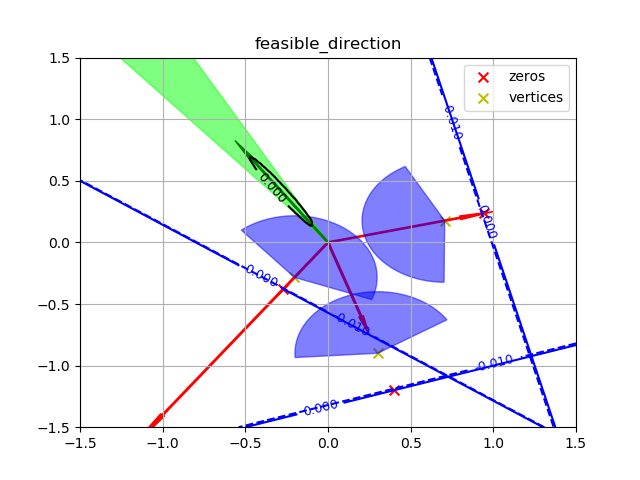
\includegraphics[width=300px]{images/feasible_direction.png}
    \caption
    	[An example of the conservative ellipsoid being overly conservative]
    	{
    		At times, the conservative ellipsoid may be much smaller than desired.
    		Here, each cone $\fik$ is in blue, and $\fcki$ is in green.
    		$\fcki$ is contained within the intersection of the $\fik$ cones.
	}
    \label{feasible_direction}
\end{figure}

We then define an ellipsoid within this cone with a helper function
\begin{align}
f_e(\epsilon, \delta, \theta; x) = (x - \epsilon e_1)^T\begin{pmatrix}
1 & \boldsymbol0^T \\
\boldsymbol 0 & \frac{\theta^2}{1 - \theta^2} \boldsymbol I \\
\end{pmatrix}(x - \epsilon e_1) - \frac 1 2 \delta^2 \label{define_ellipse_function}
\end{align}
and rotation matrix
\begin{align}
\rotk = 2\frac{(e_1 + \huk)(e_1 + \huk)^T}{(e_1 + \huk)^T(e_1 + \huk)} - \boldsymbol I \label{define_rotation}
\end{align}
by defining
\begin{align}
\gamma &= 1 + \frac 1 {\sqrt{2}} \label{define_the_constant_gamma} \\
\bs &= \max\left\{\frac 1 2 , \bsk\right\} \label{define_bs} \\
\sampletrkpo &= \left\{x \in \Rn | f_e\left(\frac 1 {2\gamma} \dkpo, \frac 1 {2\gamma} \dkpo,\bs; \rotk(x - \xkpo)\right) \le 0\right\}. \label{define_ellipsek}
\end{align}
Note that within \cref{define_ellipsek} we have defined the components $\qkpo$, $\ckpo$, $\sdkpo$ as
\begin{align}
\begin{array}{ccc}
\qkpo &=& \left(\rotk\right)^T \begin{pmatrix}
1 & \boldsymbol0^T \\
\boldsymbol 0 & \frac{\bs^2}{1 - \bs^2} \boldsymbol I \\
\end{pmatrix} \rotk, \\
\ckpo &=& \xkpo + \frac 1 {2\gamma} \dkpo \huk, \\
\sdkpo &=& \frac 1 {2\gamma} \dkpo. 
\end{array}\label{conservative_ellipsoid_details}
\end{align}

% \cref{ellsoid_is_suitable_theorem_p2} tells us that this ellipsoid satisfies \cref{ellipsoids_notation_definitions}.
% Which part? Trusted and adjacent

\subsection{Properties}
\label{feasible_ellipsoid_analysis}

In this section, we show that our construction of the set $\sampletrk$ as given in 
\cref{define_ellipsek} and \cref{define_trivial_ellipsek}
is trusted and adjacent according to definition \cref{ellipsoids_notation_definitions}.
This is shown within \cref{ellsoid_is_suitable_theorem_p1} and \cref{ellsoid_is_suitable_theorem_p2}.

\begin{lemma}
\label[lemma]{ellipse_in_cone}
Define $f_e$ by \cref{define_ellipse_function}.
Let $0 < \delta \le \epsilon$ and $\theta > 0$.

We have
\begin{align*}
\left\{x \in \Rn \bigg| f_e\left(\epsilon, \delta, \theta; x\right) \le 0\right\} \subseteq \left\{tx\in\Rn\bigg| e_1^T x \ge \theta,\|x\|=1, t>0\right\}.
\end{align*}
\end{lemma}

\begin{proof}
Let $x$ be such that $f_e(\epsilon, \delta, \theta, x) \le 0$.
First, note that a square is non-negative, so
\begin{align*}
0 \le 2(e_1^Tx - \frac 1 2 \epsilon )^2
= 2(e_1^Tx)^2 - 2e_1^Tx\epsilon + \frac 1 2 \epsilon^2.
\end{align*}
By moving the second and third terms to the right hand side, we find
\begin{align}
(e_1^Tx)^2 \ge \frac 1 2 \epsilon^2 - \left((e_1^Tx)^2 - 2e_1^Tx\epsilon + \epsilon^2\right) 
= \frac 1 2 \epsilon^2 - (e_1^Tx - \epsilon)^2. \label{ellipse_in_cone_eqn1}
\end{align}
If we substitute \cref{define_ellipse_function} into $f_e(\epsilon, \delta, \theta, x) \le 0$, we find that
\begin{align*}
(x - \epsilon e_1)^T\begin{pmatrix}
1 & \boldsymbol0^T \\
\boldsymbol 0 & \frac{\theta^2}{1 - \theta^2} \boldsymbol I \\
\end{pmatrix}(x - \epsilon e_1) \le \frac 1 2 \delta^2
\end{align*}
This can be simplified to
\begin{align*}
(x - \epsilon e_1)^T\begin{pmatrix}
1 & \boldsymbol0^T \\
\boldsymbol 0 & \frac{\theta^2}{1 - \theta^2} \boldsymbol I \\
\end{pmatrix}(x - \epsilon e_1) \\
 = (e_1^Txe_1 + (x - e_1^Txe_1) - \epsilon e_1)^T\begin{pmatrix}
1 & \boldsymbol0^T \\
\boldsymbol 0 & \frac{\theta^2}{1 - \theta^2} \boldsymbol I \\
\end{pmatrix}(e_1^Txe_1 + (x - e_1^Txe_1) - \epsilon e_1)  \\
=
(e_1^Tx - \epsilon)^2 + \frac{\theta^2}{1 - \theta^2}\|x - e_1^Tx e_1\|^2 \le \frac 1 2 \delta^2.
\end{align*}
For a contradiction, suppose that $e_1^Tx < 0$, then $(e_1^Tx - \epsilon)^2 \ge \epsilon^2 \ge \delta^2$.
However, the previous line shows $(e_1^Tx - \epsilon)^2 \le \frac 1 2 \delta^2$.
Thus, $e_1^Tx \ge 0$.
Therefore,
\begin{align*}
(e_1^Tx - \epsilon)^2 + \frac{\theta^2}{1 - \theta^2}\left(\|x\|^2 - (e_1^Tx)^2\right) 
\le (e_1^Tx - \epsilon)^2 + \frac{\theta^2}{1 - \theta^2}\|x - e_1^Tx e_1\|^2 \le \frac 1 2 \delta^2 \le \frac 1 2 \epsilon^2.
\end{align*}
Using \cref{ellipse_in_cone_eqn1}, 
\begin{align*}
\frac{\theta^2}{1 - \theta^2}(\|x\|^2 - (e_1^Tx)^2) \le \frac 1 2 \epsilon^2 - (e_1^Tx - \epsilon)^2 \le (e_1^Tx)^2
\Longrightarrow \|x\|^2 - (e_1^Tx)^2 \le \frac{1 - \theta^2}{\theta^2}(e_1^Tx)^2 \\
\Longrightarrow \|x\|^2 \le \frac 1 {\theta^2}(e_1^Tx)^2
\Longrightarrow e_1^T\frac{x}{\|x\|} \ge \theta
\end{align*}
where we can take the square root because $e_1^Tx \ge 0$.
\end{proof}

\begin{lemma}
\label[lemma]{ellipse_fits}
Define $f_e$ by \cref{define_ellipse_function}.
We have that $f_e(\delta, \sqrt{2}\delta, \theta; 0) = 0$ for any $\delta, \theta > 0$.
\end{lemma}
\begin{proof}
We compute
\begin{align*}
f_e(\delta, \sqrt{2}\delta, \theta; 0) =(0 - \delta e_1)^T\begin{pmatrix}
1 & \boldsymbol0^T \\
\boldsymbol 0 & \frac{\theta^2}{1 - \theta^2} \boldsymbol I \\
\end{pmatrix}(0 - \delta e_1) - \frac 1 2 (\sqrt 2 \delta)^2
=\delta^2 - \delta^2 = 0.
\end{align*}
% and
% \begin{align*}
% f_e(\delta, \delta, \theta; (1 + \frac{1}{\sqrt{2}}) \delta e_1) =\frac {\delta}{\sqrt{2}}e_1^T\bigg(\begin{pmatrix}
% 1 & \boldsymbol0^T \\
% \boldsymbol 0 & \frac{\theta^2}{1 - \theta^2} \boldsymbol I \\
% \end{pmatrix}\bigg)\frac {\delta}{\sqrt{2}}e_1 - \frac 1 2 \delta^2
% =\frac 1 2 \delta^2 - \frac 1 2 \delta^2 = 0.\\
% \end{align*}
\end{proof}


\begin{lemma}
\label[lemma]{ellipse_fits_part_2}
Define $f_e$ by \cref{define_ellipse_function}.

Suppose that for some $s \in \Rn$ with $\|s\| = 1$, $s^Te_1 \in \left[\frac 1 2, 1\right]$, $\delta \in [0, \frac 1 2]$ and $f_e(\delta, \delta, \theta; ts) \le 0$.

Then $t \le \left(2 + \sqrt{2}\right) \delta$.
\end{lemma}
\begin{proof}
Notice that $s^Te_1 - \delta \in \left[0, 1\right]$.
and $\left[\left(ts^Te_1 - \delta\right) e_1 + t\left(s - \left(s^Te_1\right) e_1\right)\right] = ts - \delta e_1$
so that
\begin{align*}
f_e(\delta, \delta, \theta; ts) \le 0 \\
\Longrightarrow 
\left[ts - \delta e_1\right]^T\begin{pmatrix}
1 & \boldsymbol0^T \\
\boldsymbol 0 & \frac{\theta^2}{1 - \theta^2} \boldsymbol I \\
\end{pmatrix} \left[ts - \delta e_1\right] \le \frac 1 2 \delta^2 \\
\Longrightarrow
\left(ts^Te_1 - \delta\right)^2 + t^2\left(s - \left(s^Te_1\right) e_1\right)^2  \frac{\theta^2}{1 - \theta^2} \le \frac 1 2 \delta^2 \\
\Longrightarrow 
\left(t s^Te_1 - \delta\right)^2 \le \frac 1 2 \delta^2 
\Longrightarrow t s^Te_1 - \delta \le \frac 1 {\sqrt{2}} \delta.
\end{align*}
However,
\begin{align*}
\frac 1 2 t \le t s^Te_1 \le \left(1 + \frac 1 {\sqrt{2}}\right) \delta
\Longrightarrow t \le \left(2 + \sqrt{2}\right) \delta.
\end{align*}
\end{proof}

% \Longrightarrow 
% \left[\left(ts^Te_1 - \delta\right) e_1 + t\left(s - \left(s^Te_1\right) e_1\right)\right]^T\begin{pmatrix}
% 1 & \boldsymbol0^T \\
% \boldsymbol 0 & \frac{\theta^2}{1 - \theta^2} \boldsymbol I \\
% \end{pmatrix} \\ \left[\left(ts^Te_1 - \delta\right) e_1 + t\left(s - \left(s^Te_1\right) e_1\right)\right] \le \frac 1 2 \delta^2 \\




\begin{lemma}
\label[lemma]{boundbsk}
Let $\beta$, $\bsk$, $\thetamink$, and $p_{\beta}$ be defined by \cref{define_abpab}, \cref{define_bsk}, \cref{define_thetamink}, and \cref{define_abpab}.

If $\dk^{p_{\beta}} \le \frac {1} {4\beta}\left(\thetamink\right)^2$, then $\bsk \le 1 - \frac 1 4 \left(\thetamink\right)^2$.
\end{lemma}


\begin{proof}
First note that $\thetamink \le 1$ and $p_{\beta} \in (0, 1)$, so that $\beta \dk \le \frac 1 4$.
Because $\left(\thetamink\right)^2 \ge 4\beta\dk^{p_{\beta}}$,
\begin{align*}
    \left[1 - \left(\beta \dk ^{p_{\beta}}\right)^2\right]\left[1 - \left(\thetamink \right)^2\right]
\le \left[1 - \left(\beta \dk ^{p_{\beta}}\right)^2\right]\left[1 - 4\beta \dk^{p_{\beta}}\right] \\
= 1 - 4 \beta \dk^{p_{\beta}} - \left(\beta \dk^{p_{\beta}}\right)^2 + 4 \left(\beta \dk^{p_{\beta}}\right)^3 \\
= \left(1 - 2 \beta \dk^{p_{\beta}}\right)^2 - 5 \left(\beta\dk^{p_{\beta}}\right)^2 + 4 \left(\beta \dk^{p_{\beta}}\right)^3 \\
\le \left(1 - 2\beta\dk^{p_{\beta}}\right)^2.
\end{align*}
Thus, 
\begin{align}
\label{steves_rewrite_eqn1}
\sqrt{\left[1 - \left(\beta \dk ^{p_{\beta}}\right)^2\right]\left[1 - \left(\thetamink \right)^2\right]} 
\le 1 - 2 \beta \dk^{p_{\beta}}.
\end{align}
Note also that $1 - \left(\beta  \dk ^{p_{\beta}}\right)^2 \le 1$, so
\begin{align}
\label{steves_rewrite_eqn2}
\sqrt{\left[1 - \left(\beta \dk ^{p_{\beta}}\right)^2\right]\left[1 - \left(\thetamink \right)^2\right]} 
\le \sqrt{1 - \left(\thetamink \right)^2} \le 1 - \frac 1 2 \left(\thetamink \right)^2.
\end{align}
Adding \cref{steves_rewrite_eqn1} and \cref{steves_rewrite_eqn2}, we find
\begin{align*}
2 \sqrt{\left[1 - \left(\beta \dk ^{p_{\beta}}\right)^2\right]\left[1 - \left(\thetamink \right)^2\right]} 
\le 2 - 2 \beta \dk ^{p_{\beta}} - \frac 1 2 \left(\thetamink \right)^2
\end{align*}
and
\begin{align*}
\bsk = \beta \dk ^{p_{\beta}} + \sqrt{\left[1 - \left(\beta \dk ^{p_{\beta}}\right)^2\right]\left[1 - \left(\thetamink \right)^2\right]}
\le \beta \dk ^{p_{\beta}} + 1 - \beta \dk ^{p_{\beta}} - \frac 1 4 \left(\thetamink \right)^2 \\
= 1 - \frac 1 4 \left(\thetamink \right)^2.
\end{align*}
\end{proof}

% \begin{proof}
% For any $0 < \epsilon < 1$ there exists $\dacco(\epsilon) > 0$, such that for any $k \in \naturals$ with
% $\thetamink \ge \epsilon$ and $\dk \le \dacco(\epsilon)$, we have
% $\bsk \le 1 - \frac 1 4 \epsilon^2$.
% Let $\alpha$, $\beta$, $p_{\alpha}$, and $p_{\beta}$ be defined by \cref{define_abpab}.
% % Also, let $\minangledelta$ be defined as in \cref{minangleassumption}.
% Then we can let $\dacco(\epsilon)$ be defined by
% % \minangledelta,
% % 1,
% \begin{align}
% \dacco(\epsilon) < \min\left\{
% \left(\frac {\epsilon ^2} {4\beta} \right)^{\frac 1 {p_{\beta}}},
% \left(\frac 1 {2\beta}\right)^{\frac 1 {p_{\beta}}}
% \right\}\label{define_delta_accuracy_old}.
% \end{align}
% If $\dk \le \dacco(\epsilon)$, then
% \begin{align}
% \beta\dk^{p_{\beta}} \le \frac 1 {4} \epsilon^2 \quad \textrm{and}\label{boundedbeta_deltasmall_2} \\
% 2\beta\dk^{p_{\beta}} \le 1. \label{boundedbeta_deltasmall_3}
% \end{align}
% Rearranging \cref{boundedbeta_deltasmall_2}, provides $-\epsilon^2 \le -4\beta\dk^{p_{\beta}}$,
% which combined with $\epsilon ^2 \le 1 \le 5$ shows
% \begin{align*}
% -\left[5- \epsilon^2\right]\left(\beta\dk^{p_{\beta}}\right)^2  - \epsilon^2 \le -4\beta\dk^{p_{\beta}}.
% \end{align*}
% This means
% \begin{align*}
% \left(1 - \epsilon^2\right)\left(1 - \left(\beta\dk^{p_{\beta}}\right)^2\right) 
% = 1 - \epsilon^2 - \left[5 - \epsilon^2\right]\left(\beta\dk^{p_{\beta}}\right)^2 + 4\left(\beta\dk^{p_{\beta}}\right)^2 \\
% \le 1 - 4\beta\dk^{p_{\beta}} + 4\left(\beta\dk^{p_{\beta}}\right)^2 = \left(1 - 2\beta\dk^{p_{\beta}}\right)^2.
% \end{align*}
% Dividing by $1 - \left(\beta\dk^{p_{\beta}}\right)^2$, taking the square root, and then dividing by $2$ we see
% % 1 - \epsilon^2 \le \frac{\left(1 - 2\beta\dk^{p_{\beta}}\right)^2}{1 - \left(\beta\dk^{p_{\beta}}\right)^2}
% % \Longrightarrow
% \begin{align}
% \frac 1 2 \sqrt{1 - \epsilon^2} \le \frac 1 2 \frac{1 -2\beta\dk^{p_{\beta}}}{\sqrt{1 - \left(\beta\dk^{p_{\beta}}\right)^2}}
% = \frac{\frac 1 2 -\beta\dk^{p_{\beta}}}{\sqrt{1 - \left(\beta\dk^{p_{\beta}}\right)^2}}. \label{boundedbeta_eqn1}
% \end{align}
% Here, \cref{boundedbeta_deltasmall_3} ensures that the denominator is positive.
% Also,
% \begin{align*}
% 1 - \epsilon^2 \le 1 - \epsilon^2 + \frac 1 4 \epsilon^4 
% = \left(1 - \frac 1 2 \epsilon^2 \right)^2 
% \Longrightarrow 1 \le \frac{\left(1 - \frac 1 2 \epsilon^2\right)^2}{1 - \epsilon^2}
% \end{align*}
% so that
% \begin{align*}
% 1 - \left(\beta\dk^{p_{\beta}}\right)^2 \le 1 \le \frac{\left(1 - \frac 1 2 \epsilon^2\right)^2}{1 - \epsilon^2} 
% \Longrightarrow \sqrt{1 - \left(\beta\dk^{p_{\beta}}\right)^2}\le \frac{1 - \frac 1 2 \epsilon^2}{\sqrt{1 - \epsilon^2} } 
% \Longrightarrow \sqrt{1 - \epsilon^2} \le \frac{1 - \frac 1 2 \epsilon^2}{\sqrt{1 - \left(\beta\dk^{p_{\beta}}\right)^2}}.
% \end{align*}
% Dividing by $2$ yields:
% \begin{align}
% \frac 1 2 \sqrt{1 - \epsilon^2} \le \frac{\frac 1 2 - \frac 1 4 \epsilon^2}{\sqrt{1 - \left(\beta\dk^{p_{\beta}}\right)^2}}
% \label{boundedbeta_eqn2}.
% \end{align}
% 
% We then add \cref{boundedbeta_eqn1} and \cref{boundedbeta_eqn2} to find
% \begin{align*}
% \sqrt{1 - \epsilon^2} \le \frac{1 -  \frac 1 4 \epsilon^2 - \beta\dk^{p_{\beta}}}{\sqrt{1 - \left(\beta\dk^{p_{\beta}}\right)^2}}
% \Longrightarrow \beta\dk^{p_{\beta}} + \left(\sqrt{1 - \epsilon^2}\right)\sqrt{1 - \left(\beta\dk^{p_{\beta}}\right)^2} \le 1 -  \frac 1 4 \epsilon^2.
% \end{align*}
% Because $\thetamink \ge \epsilon$, we have $\sqrt{1 - \epsilon^2} \ge \sqrt{1 - \left(\thetamink\right)^2}$
% so that
% \begin{align*}
% \bsk 
% = \beta\dk^{p_{\beta}} + \sqrt{\left(1 - \left(\beta\dk^{p_{\beta}}\right)^2\right)\left(1 - \left(\thetamink\right)^2\right)} 
% \le \beta\dk^{p_{\beta}} + \left(\sqrt{1 - \epsilon^2}\right)\sqrt{1 - \left(\beta\dk^{p_{\beta}}\right)^2} \\
% \le 1 -  \frac 1 4 \epsilon^2.
% \end{align*}
% \end{proof}



\begin{lemma}
\label[lemma]{boundbeta}
Let $\beta$, $\thetamink$, and $\qkpo$ be defined by \cref{define_abpab}, \cref{define_thetamink}, and \cref{define_ellipsek} respectively.

If $\dk \le \frac 1 {4 \beta} \left(\thetamink\right)^2$, then $\condition \left(\qkpo\right) \le 12 \left(\thetamink\right)^{-2}$.

% For any $0 < \epsilon < 1$ there exists $\dacco(\epsilon) > 0$, such that for any $k \in \naturals$ with
% $\thetamink \ge \epsilon$ and $\dk \le \dacco(\epsilon)$, we have $\condition\left(\qkpo\right) \le \frac{12}{\epsilon^2}$.
\end{lemma}

\begin{proof}
Let $\rotk$, and $\gamma$ be defined as in \cref{define_rotation}, and \cref{define_the_constant_gamma} respectively.
Also, during iteration $k$, let $\bs$ be defined by \cref{define_bs}.
% Definition \cref{define_ellipsek} states
% \begin{align*}
% \qk = \rotk^T \begin{pmatrix}
% 1 & \boldsymbol0^T \\
% \boldsymbol 0 & \frac{\bs^2}{1 - \bs^2} \boldsymbol I \\
% \end{pmatrix} \rotk, \quad
% \ck = \xk  + \frac 1 {2\gamma} \dk\huk, \quad
% \sdk = \frac 1 {2\gamma} \dk.
% \end{align*}
First note that by \cref{define_bs} and \cref{boundbsk}, we have
$\frac 1 2 \bsk \le 1 - \frac 1 4 \left(\thetamink\right)^2$.
Squaring this yields
\begin{align}
\frac {1} 4 \le \left(\bs\right)^2 \le \left(1 - \frac 1 4 \left(\thetamink\right)^2\right)^2 \le 1 - \frac 1 4 \left(\thetamink\right)^2 \label{p2_numerator}
\end{align}
so that
\begin{align}
\frac 1 4  \left(\thetamink\right)^2 \le 1 - \left(\bs\right)^2 \le \frac 3 4. \label{p2_denominator}
\end{align}
Dividing \cref{p2_numerator} by \cref{p2_denominator}, we see that
\begin{align*}
\frac 1 3
\le \frac{\left(\bs\right)^2}{1 - \left(\bs\right)^2}
\le \frac {4 - \left(\thetamink\right)^2}{\left(\thetamink\right)^2} \le \frac {4}{\left(\thetamink\right)^2}
\end{align*}
Now, using \cref{conservative_ellipsoid_details}, we can compute 
\begin{align*}
\condition \left(\qkpo\right) 
= \frac{\max\left\{1, \frac{\left(\bs\right)^2}{1 - \left(\bs\right)^2}\right\}}{\min\left\{1, \frac{\left(\bs\right)^2}{1 - \left(\bs\right)^2}\right\}} 
\le \frac {12}{\left(\thetamink\right)^2}
\end{align*}
as $\det(\rotk) = 1$.
\end{proof}




\begin{lemma}
\label[lemma]{cone_subset_cone}
Given $u, v \in \Rn$, and $\gamma \in (0, 1]$, $\beta \in [0, \gamma)$ that satisfy $\|u\| = \|v\|= 1$, $u^Tv = \gamma$, define
\begin{align*}
B = \{x\in\Rn | {v}^Tx \ge \beta\|x\|\}, \quad
S = \left\{x\in\Rn \bigg| u^Tx \ge \left(\beta\gamma + \sqrt{(1 - \beta^2)\left(1 - \gamma^2\right)}\right)\|x\| \right\}. 
\end{align*}
Then, $S \subseteq B$.
\end{lemma}

\begin{proof}
For a contradiction, let $y \in \Rn$ be such that $y \not \in B$ and $y \in S$ and define $\hat y = \frac{y}{\|y\|}$.
That is,
\begin{align}
v^T\hat y < \beta \label{csc_vy} \\
u^T\hat y \ge \beta\gamma + \sqrt{\left(1 - \beta^2\right)\left(1 - \gamma^2\right)}. \label{csc_uy}
\end{align}

Define
\begin{align*}
x^{\star} = \beta v + \sqrt{\frac{1 - \beta^2}{1 - \gamma^2}} (u - \gamma v )
\end{align*} and notice
\begin{align}
\begin{array}{ccccc}
{u}^Tx^{\star} &=& \beta\gamma + \sqrt{\frac{1 - \beta^2}{1 - \gamma^2}} (1 - \gamma^2) &=&  \beta\gamma + \sqrt{\left(1 - \beta^2\right)\left(1 - \gamma^2\right)} \\
{v}^Tx^{\star} &=& \beta + \sqrt{\frac{1 - \beta^2}{1 - \gamma^2}}(\gamma - \gamma) &=& \beta \\
{x^{\star}}^Tx^{\star} &=& \beta^2 + 2\beta\sqrt{\frac{1 - \beta^2}{1 - \gamma^2}}(\gamma - \gamma) + \frac{1 - \beta^2}{1 - \gamma^2} (1- 2\gamma^2 + \gamma^2)&=& 1.
\end{array}. \label{csc_vx_ux}
\end{align}

Using \cref{csc_vx_ux} and \cref{csc_uy}, we see
\begin{align*}
\beta\gamma + \sqrt{\left(1 - \beta^2\right)\left(1 - \gamma^2\right)} \le {u}^T\hat y = {u}^T\left(x^{\star} + \hat y - x^{\star}\right) \\
= \beta \gamma + \sqrt{(1 - \beta^2)\left(1 - \gamma^2\right)} + {u}^T\left(\hat y - x^{\star}\right).
\end{align*}
Subtracting $\beta\gamma + \sqrt{\left(1 - \beta^2\right)\left(1 - \gamma^2\right)}$ from both sides, we find
\begin{align}
{u}^T\left(\hat y - x^{\star}\right) \ge 0 \label{csc_uymx}.
\end{align}
Likewise, we can use \cref{csc_vx_ux} and \cref{csc_vy} to provide
\begin{align*}
\beta > {v}^T\hat y = {v}^T\left(x^{\star} + \hat y - x^{\star}\right) = \beta + {v}^T\left(\hat y - x^{\star}\right).
\end{align*}
After subtracting $\beta$ from both sides, we see
\begin{align}
{v}^T\left(\hat y - x^{\star}\right) < 0 \Longrightarrow -{v}^T\left(\hat y - x^{\star}\right) > 0. \label{csc_vymx}
\end{align}
% which means $\hat y \ne x^{\star}$.
Lastly, we will need
\begin{align}
\gamma > \beta 
\Longrightarrow 1 - \beta^2 > 1 - \gamma^2
\Longrightarrow \sqrt{\frac{1 - \beta^2}{1 - \gamma^2}} > 1
\Longrightarrow \gamma \sqrt{\frac{1 - \beta^2}{1 - \gamma^2}} - \beta > 0. \label{csc_gamma_beta_positive}
\end{align}
Now, we can compute
\begin{align*}
{\left(\hat y - x^{\star}\right)}^Tx^{\star} = 
\beta {\left(\hat y - x^{\star}\right)}^Tv
+ \sqrt{\frac{1 - \beta^2}{1 - \gamma^2}} 
\left(u^T\left(\hat y - x^{\star}\right) - \gamma v^T \left(\hat y - x^{\star}\right) \right)\\ 
= \left[\gamma \sqrt{\frac{1 - \beta^2}{1 - \gamma^2}} - \beta\right] \left[-v^T\left(\hat y - x^{\star}\right)\right]
+ \left[\sqrt{\frac{1 - \beta^2}{1 - \gamma^2}}\right] \left[u^T\left(\hat y - x^{\star}\right) \right] > 0.
\end{align*}
because \cref{csc_uymx}, \cref{csc_vymx}, and \cref{csc_gamma_beta_positive} show that the first product is postive and the second product is non-negative.
However, this is a contradiction as
\begin{align*}
1 = \|\hat y\|^2 = \|x^{\star} + \hat y - x^{\star}\|^2 = \|x^{\star}\|^2 + 2{\left(\hat y - x^{\star}\right)}^Tx^{\star} + \|\hat y - x^{\star}\|^2 > \|x^{\star}\|^2 = 1
\end{align*}
and there is no such $y$.
Thus, any $y \in\Rn$ with $y \in S$ must also have $y \in B$.
\end{proof}


\begin{lemma}
\label[lemma]{large_zik_means_means_no_intersection}
Let
$\zik$ and $\fik$
be defined by
\cref{define_z} and \cref{define_fik} respectively.
For any $R > 0$ and $K > R\sqrt{n}$, there exists $\deltalargzik > 0$ such that if $\dk \le \deltalargzik$ and 
\begin{align*}
\zik \not \in B_{\infty}\left(\xk, (1+K) \dk\right),
\end{align*}
then $B_{\infty}\left(\xk, R \dk\right) \subseteq \fik$.
\end{lemma}
\begin{proof}
Let $\alpha$, $\beta$, $p_{\alpha}$, and $p_{\beta}$ be defined by \cref{define_abpab}.
We can define
\begin{align}
\deltalargzik = \min\left\{
\left(\frac 1 {\beta }\frac {K - R\sqrt{n}}{K + R\sqrt{n}}\right)^{\frac 1 {p_{\beta }}},
\left(\frac 1 {(1+K)\alpha}\right)^{\frac 1 {p_{\alpha}}}
\right\} \label{define_deltalargzik}
\end{align}
and suppose that $\|\xk - \zik\| \ge (1+K) \dk$.

First, note that by \cref{define_w}
\begin{align*}
\|\xk - \wik\| = (1 - \alpha\dk^{p_{\alpha}}) \|\xk - \zik\| \ge \frac {K} {(1+K)} (1+K)\dk = K\dk.
\end{align*}

Let $y \in B_{\infty}\left(\xk, R \dk\right)$, so that $\|y - \xk\| \le \sqrt{n}R\dk$.
Also, define
\begin{align*}
t  = \frac{(y - \wik)^T(\xk - \wik)}{\left(\xk - \wik\right)^T(\xk - \wik)} \\
p = \wik + t\left(\xk - \wik\right)
\end{align*}
so that
\begin{align*}
\|y - \wik\| \le \|y - \xk\| + \|\xk - \wik\| \\
\Longrightarrow \frac{\|y - \wik\|}{\|\xk - \wik\|} \le 1 +  \frac{\|y - \xk\|}{\|\xk - \wik\|} 
\le 1 + \frac{\sqrt{n}R\dk}{K \dk} = \frac {K+R\sqrt{n}}{K} \\
\Longrightarrow \frac{\|\xk - \wik\|}{\|y - \wik\|} \ge \frac {K}{K+R\sqrt{n}}
\end{align*}
and
\begin{align*}
\left(y - p\right)^T\left(\xk - \wik\right) = 
\left(y - \wik - t\left(\xk - \wik\right)\right)^T\left(\xk - \wik\right) \\
= \left(y - \wik\right)^T\left(\xk - \wik\right) - t\left(\xk - \wik\right)^T\left(\xk - \wik\right) = 0.
\end{align*}
Because
\begin{align*}
\|\xk - p\| = \|\xk - \wik + \wik - p\| = \left\|\xk - \wik - t\left(\xk - \wik\right)\right\| \\
= (1-t)\|\xk - \wik\| \ge (1-t)K\dk
\end{align*}
we have
\begin{align*}
nR^2\dk^2 \ge \|\xk - y\|^2 = \|\xk - p\|^2 + \|y - p\|^2 \ge K^2(1-t)^2\dk^2  \\
\Longrightarrow 1-t \le \frac {R\sqrt{n}} {K} 
\Longrightarrow t \ge \frac {K - R\sqrt{n}}{K}
\end{align*}

Putting this together, we see
\begin{align*}
\frac{\xk - \wik}{\left\|\xk - \wik\right\|}^T\frac{y - \wik}{\left\|y - \wik\right\|} 
= \frac{\left(\xk - \wik\right) ^T\left(y - p\right) + \left(\xk - \wik\right)^T\left(p - \wik\right)}{\left\|\xk - \wik\right\|\left\|y - \wik\right\|} \\
= t\frac{\left(\xk - \wik\right)^T\left(\xk - \wik\right)}{\left\|\xk - \wik\right\|\left\|y - \wik\right\|}
= t \frac{\left\|\xk - \wik\right\|}{\left\|y - \wik\right\|}
= \frac {K - R\sqrt{n}}{K + R\sqrt{n}} \ge \beta \dk^{p_{\beta}}.
\end{align*}
% \ge \frac {K - \sqrt{n}}{K} \frac {K}{K+\sqrt{n}}
\end{proof}

\begin{lemma}
\label[lemma]{inner_cone_inside_each_cone}
Let $\fcki$ and $\capcones$ be defined by \cref{define_inner_cone} and \cref{define_capcones} respectively.
If 
% $\dk \le 1$ and 
$\xkpo \in \capcones$, then $\fcki \subseteq \capcones$.
\end{lemma}
% \left(\frac 1 {\beta} \sqrt{\frac 3 4}\right)^{\frac 1 {p_{\beta}}}

\begin{proof}
Let 
$\huk$, $\bsk$, $\thetamink$, $\activeconstraintsk$, and $\fik$
be defined by
\cref{define_u}, \cref{define_bsk}, \cref{define_thetamink}, \cref{define_activeconstraints}, and \cref{define_fik} 
respectively and $\alpha$, $\beta$, $p_{\alpha}$, $p_{\beta}$ be defined by \cref{define_abpab}.
Fix some $i \in \activeconstraintsk$, and define $\gamma_i = -\left(\huk\right)^T\hgik$ as well as
\begin{align*}
S_1 = \left\{s\in\Rn | \quad s^T\huk\ge\bsk\|s\| \right\} \\
S_2 = \left\{s\in\Rn | \quad s^T\huk\ge\left[\beta\dk^{p_{\beta}}\gamma_i + \sqrt{(1 - \left(\dk^{p_{\beta}}\beta\right)^2)\left(1 - \gamma_i^2\right)}\right]\|s\| \right\} \\
S_3 = \left\{s\in\Rn | \quad s^T\left(-\hgik\right)\ge\beta\dk^{p_{\beta}}\|s\| \right\}
\end{align*}
The set $S_1$ is that set of all feasible directions from $\xk$ for $\fcki$, and $S_3$ is that set of all feasible direction from $\wik$ for $\fik$.
Because $\xkpo \in \fik$, $\fcki \subseteq \fik$ follows from $S_1 \subseteq S_3$.
We show this next.


% = -\frac{m_{c_i}(\xk)}{\|\gmcik\|}\frac{\|\gmcik\|}{m_{c_i}(\xk)}
% Now, we show that $S_1 \subseteq S_3$.
By letting $u \gets \huk$, $v \gets -\hgik$, $\beta \gets \beta \dk^{p_{\beta}}$, \cref{cone_subset_cone} tells us that
$S_2 \subseteq S_3$.
But $\gamma_i \ge \thetamink$, so that
\begin{align*}
\beta\dk^{p_{\beta}}\gamma_i + \sqrt{\left(1 - \left(\beta\dk^{p_{\beta}}\right)^2\right)\left(1 - \gamma_i^2\right)}
\le \max_{i\in\activeconstraintsk} \left(\beta\dk^{p_{\beta}}\gamma_i + \sqrt{\left(1 - \left(\beta\dk^{p_{\beta}}\right)^2\right)\left(1 - \gamma_i^2\right)}\right) \\
\le \beta\dk^{p_{\beta}} \max_{i\in\activeconstraintsk}\left\{\gamma_i\right\} + \sqrt{\left(1 - \left(\beta\dk^{p_{\beta}}\right)^2\right)\left(1 - \left(\min_{i\in\activeconstraintsk}\left\{\gamma_i\right\}\right)^2\right)} \\
\le \beta\dk^{p_{\beta}} + \sqrt{\left(1 - \left(\beta\dk^{p_{\beta}}\right)^2\right)\left(1 - \left(\thetamink\right)^2\right)} = \bsk
\end{align*}

and for any $s\in S_1$,
\begin{align*}
\left(\frac{s}{\|s\|}\right)^T\huk \ge \bs 
\ge \beta\dk^{p_{\beta}}\gamma_i + \sqrt{(1 - \dk^{2p_{\beta}}\beta^2)\left(1 - \gamma_i^2\right)}
\Longrightarrow s \in S_2 \subseteq S_3.
\end{align*}

Thus, $\fcki \subseteq \fik$.
\end{proof}


% \color{red}
% The red is no longer needed.
% First, we show that $\xk \in \fik$.
% We see that:
% \begin{align*}
% \xk = \xk + \left(1 - \alpha\dk^{p_{\alpha} }\right)(\zik - \xk) - \left(1 - \alpha\dk^{p_{\alpha} }\right)(\zik - \xk)
% \end{align*}
% where
% \begin{align*}
% \frac{-\left(1 - \alpha\dk^{p_{\alpha} }\right)(\zik - \xk)}{\left\|-\left(1 - \alpha\dk^{p_{\alpha} }\right)(\zik - \xk)\right\|}^T\hgik = 1 \ge \beta \dk^{p_{\beta}}
% \end{align*}
% because $\dk \le 1$.
% \color{black}


\begin{lemma}
\label[lemma]{ellsoid_is_suitable_theorem_p1}
Let $\activeconstraintsk$ and $\omegainc$ be defined by \cref{define_activeconstraints} and \cref{define_the_omegas} respectively.
If $\activeconstraintsk = \emptyset$ and $\dkpo \le \omegainc\dk$, 
then there exists $\deltalargzik>0$ such that if $\dk \le \deltalargzik$ the
ellipsoids defined by \cref{define_trivial_ellipsek} 
are trusted, and adjacent according to \cref{ellipsoids_notation_definitions}.

% satisfy \cref{ellipsoids_notation_definitions}.
\end{lemma}
\begin{proof}
Also, \cref{define_suitable_close_to_iterate} is satisfied because $(\xkpo - \xkpo)^T\qkpo(\xkpo - \xkpo) = 0 \le \sdkpo^2$.
Let $\omegainc$, $\capcones$, $\fik$, and $\zikthresh$ be defined by \cref{define_the_omegas}, \cref{define_capcones}, \cref{define_fik}, and \cref{define_zikthresh} respectively.
Because $\activeconstraintsk = \emptyset$, we can use 
\cref{large_zik_means_means_no_intersection} with $R = (2 + \omegainc)\sqrt{n}$, $K = \zikthresh$ to conclude the existence of $\deltalargzik > 0$ such that 
if $\dk \le \deltalargzik$, then for each 
$i \in [m]$, $\trkpo \subseteq \fik$.
Thus, \cref{define_suitable_in_tr} is satisfied because 
\begin{align*}
\unshiftedellipsoidkpo = \left\{x \in \Rn \bigg| \|x - \xkpo\|^2 \le \dkpo^2 \right\} \subseteq \trkpo \subseteq \capcones.
\end{align*}
\end{proof}


\begin{lemma}
\label[lemma]{ellsoid_is_suitable_theorem_p2}
Let $\activeconstraintsk$ 
% and $\omegainc$ 
be defined by 
\cref{define_activeconstraints}
% and \cref{define_the_omegas} respectively
.
If $\activeconstraintsk \ne \emptyset$ and $\dk \le 1$, 
then the ellipsoids defined by \cref{define_ellipsek} are trusted and adjacent according to \cref{ellipsoids_notation_definitions}.

% There exsists $\dacc > 0$ such that if $\dk \le \dacc$
% and $\activeconstraintsk \ne \emptyset$
% \begin{align}
% \bs = \max\left\{\frac 1 2, \bsk\right\} \label{define_bs} \\
% \gamma = 1 + \frac 1 {\sqrt 2}
% \end{align}
% where $\dacc$ is defined in \cref{define_delta_accuracy}, and $\rotk$ be defined as in \cref{define_rotation}.
% Then, \cref{ellipsoids_notation_definitions} is satisfied by letting
% as in \cref{define_ellipsek}.
\end{lemma}
\begin{proof}
Let $\rotk$, $\gamma$, $f_e$, and $\bs$ be defined as in \cref{define_rotation}, \cref{define_the_constant_gamma}, \cref{define_ellipse_function}, and \cref{define_bs} respectively.
% Definition \cref{define_ellipsek} states
% \begin{align*}
% \qk = \rotk^T \begin{pmatrix}
% 1 & \boldsymbol0^T \\
% \boldsymbol 0 & \frac{\bs^2}{1 - \bs^2} \boldsymbol I \\
% \end{pmatrix} \rotk, \quad
% \ck = \xk  + \frac 1 {2\gamma} \dk\huk, \quad
% \sdk = \frac 1 {2\gamma} \dk.
% \end{align*}
Because $\rotk\huk = e_1$, we have for any $\delta > 0$:
\begin{align*}
\left(x - \ckpo\right)^T\qkpo\left(x - \ckpo\right) - \frac 1 2 \delta^2 
= \left(\rotk\left(x-\xkpo\right) - \frac 1 {2\gamma} \dkpo e_1\right)^T \\ \begin{pmatrix}
1 & \boldsymbol0^T \\
\boldsymbol 0 & \frac{\left(\bs\right)^2}{1 - \left(\bs\right)^2} \boldsymbol I \\
\end{pmatrix} \left(\rotk\left(x-\xkpo\right) - \frac 1 {2\gamma} \dkpo e_1\right) - \frac 1 2 \delta^2 \\
= f_e\left(\frac 1 {2\gamma} \dkpo, \delta, \bs; \rotk\left(x - \xkpo\right)\right).
\end{align*}

% This used to be a line, but it was too long...
% = \left(x - \left(\xkpo + \frac 1 2 \dkpo \huk\right)\right)^T\rotk^T\begin{pmatrix}
% 1 & \boldsymbol0^T \\
% \boldsymbol 0 & \frac{\left(\bs\right)^2}{1 - \left(\bs\right)^2} \boldsymbol I \\
% \end{pmatrix} \rotk\left(x - \left(\xkpo + \frac 1 2 \dkpo \huk\right)\right) - \frac 1 2 \delta^2 \\


In particular, with definitions \cref{define_unshifed_ellipsoid} and \cref{define_scaledunshiftedellipsoid},
we can let $\delta = \sdkpo$ and $\delta = \sqrt{2}\sdkpo$ to see that with $s = x - \xkpo$
\begin{align*}
\unshiftedellipsoidpo = \left\{\xkpo + s \in \Rn | f_e\left(\frac 1 {2\gamma} \dkpo, \frac 1 {2\gamma} \dkpo, \bs; \rotk s \right) \le 0 \right\} \\
\scaledunshiftedellipsoidpo = \left\{\xkpo + s \in \Rn | f_e\left(\frac 1 {2\gamma} \dkpo, \sqrt{2} \frac {1}{2\gamma}\dkpo, \bs; \rotk s\right) \le 0 \right\}.
\end{align*}
With $y = \rotk s$,  we can use \cref{ellipse_in_cone} to conclude
\begin{align*}
\unshiftedellipsoidpo
\subseteq \xkpo + \rotk\left\{y \in \Rn | f_e\left(\frac 1 {2\gamma} \dkpo, \frac 1 {2\gamma} \dkpo, \bs; y \right) \le 0 \right\} \\
\subseteq  \xkpo + \rotk \left\{t y \in \Rn \bigg| e_1^Ty \ge \bs, \left\|y\right\| = 1, t > 0 \right\} \\
= \xkpo + \left\{t s \in \Rn \bigg| e_1^T\rotk s \ge \bs, \left\|\rotk s\right\| = 1, t > 0 \right\} \\
= \left\{x  \in \Rn \bigg| x = \xkpo + ts, s^T\huk \ge \bs, \|s\| = 1, t > 0 \right\}
\end{align*}
% .
% \end{align*}
% % because $\bs \ge \bsk$ and $\frac 1 {2\gamma} \dkpo \le \frac 1 {2\gamma} \dkpo$.
% % With a change of variables $s \gets x - \xkpo$, we see that
% \begin{align*}

as $\rotk = \rotk^T$.
Because $\bs \ge \bsk$ and $\bs \ge \frac 1 2$, we know two things:
\begin{align*}
\unshiftedellipsoidpo \subseteq \left\{x \in \Rn | x = \xkpo + ts, s^T\huk \ge \frac 1 2, \|s\|= 1, t > 0 \right\} \\
\textrm{and} \quad \unshiftedellipsoidpo \subseteq \left\{x \in \Rn | x = \xkpo + ts, s^T\huk \ge \bsk, \|s\|= 1, t > 0 \right\} = \fcki
\end{align*}
where $\fcki$ is defined by \cref{define_inner_cone}.
Thus, for any $x \in \unshiftedellipsoidpo$, we can let $x = \xkpo + ts$, $\|s\| = 1$, $s^T\huk \ge \frac 1 2$.
Because $\frac 1 2 \dkpo \le \frac 1 2$, we can apply \cref{ellipse_fits_part_2} to conclude $\|x - \xkpo\| = t \le \left(2 + \sqrt{2}\right)\frac 1 {2\gamma} \dkpo = \dkpo$.
Thus, $x \in \trkpo$, and $\unshiftedellipsoidpo \subseteq \fcki \cap \trkpo$.
By \cref{inner_cone_inside_each_cone}, $\fcki \subseteq \capcones$ and \cref{define_suitable_in_tr} is satisfied.
For \cref{define_suitable_close_to_iterate}, \cref{ellipse_fits} tells us that
$f_e\left(\frac 1 {2\gamma} \dkpo, \frac 1 {\sqrt{2}\gamma}\dkpo, \bs; \rotk\left(\xkpo - \xkpo\right)\right) = 0$, so that $\xkpo \in \scaledunshiftedellipsoidpo$.
\end{proof}



\section{Infeasible Trial Points}
\label{convex_model_reduction}

The second instance that the algorithm may attempt to evaluate an infeasible point is after solving the trust region subproblem.
We have two methods for dealing with this case.

\subsection{Linear cuts}
\label{linear_cuts_section}
One strategy is to solve the trust region subproblem again, after adding a linear constraint that removes this infeasible point.
Each new linear constraint not only cuts off the last trial point, but also stays at least a fraction of the trust region radius away.

\begin{figure}[ht]
    \centering
    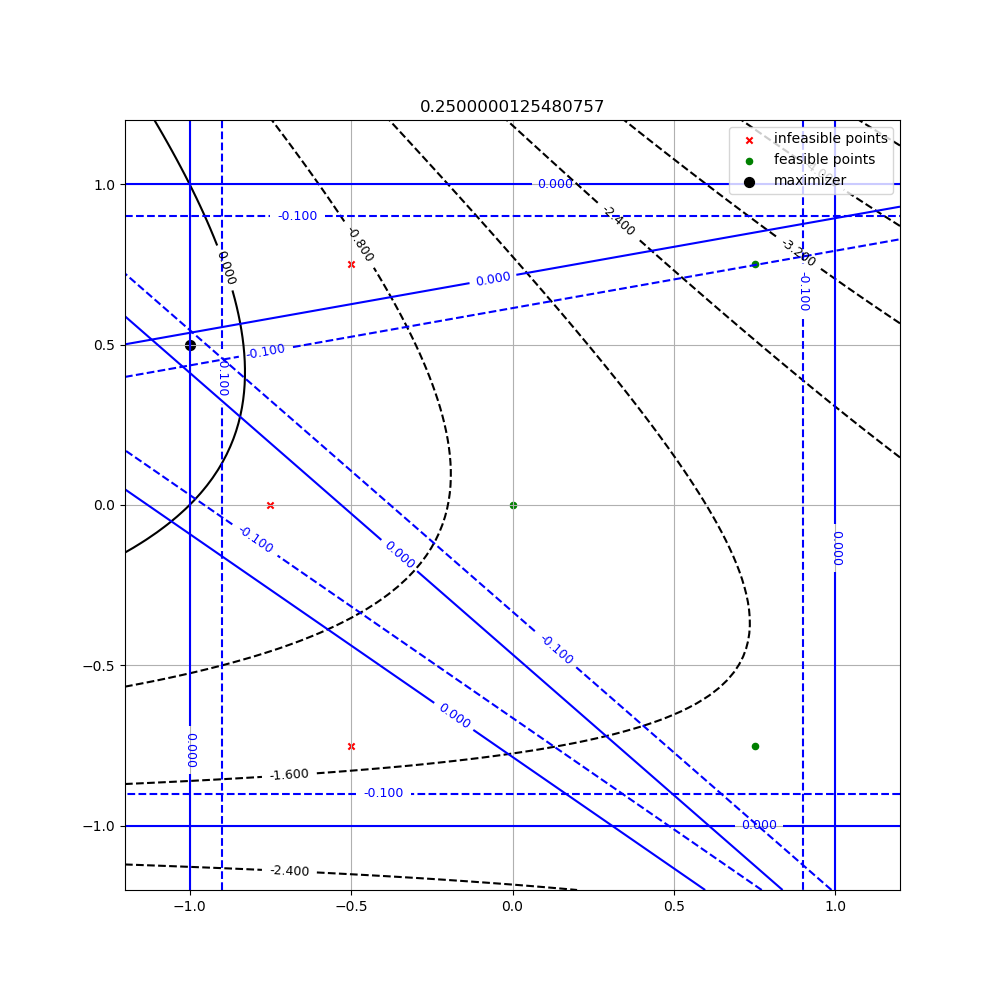
\includegraphics[width=300px]{images/pyomo_cut_solution.png}
    \caption
    		[Infeasible points can be removed from the search with linear cuts.]
    	{
			Adding linear cuts to remove infeasible points.
			Sample points that have already been evaluated and found to be feasible are shown as green circles.
			Attempted evaluations that resulted in infeasible evaluations are shown as red x's.
			The linear cuts (blue lines) are chosen to minimize the value of the objective (in black) while ensuring that all failed evaluations are infeasible.
	}
    \label{pvip}
\end{figure}


Suppose that the algorithm has evaluated several infeasible points after solving the trust region subproblem.
These are stored in a set $\trsinfset = \{n_1, n_2, \ldots, n_{|\trsinfset|}\}$.
We then choose one hyperplane $\{x \in \Rn | d_k^Tx = b_k\}$ for each infeasible point to remove that feasible point from our next attempt to solve the trust region subproblem.
Notice that these hyperplanes are \emph{decision variables} during the next attempt, so as to give as much freedom for our next trial solution.

If we let $\trstol \in (0, 1)$ be the percentage of the trust region radius with which we wish buffer our next solution, 
we arrive at the following optimization problem with $\searchtrk = \capcones \cap \tr $:
\begin{align}
\label{buffered_trust_region_subproblem}
\begin{array}{ccc}
\sk = \argmin_{s, d^{(k)} \in \Rn, b_i \in \reals}	& \mfk(x) & 	\\
 \mbox{subject to}  & n_k^Td^{(k)} \ge b_k + \trstol \dk& \forall k \in \left[ |\trsinfset |\right] \\
 & s^T d^{(k)} \le b_k &   \forall k \in \left[|\trsinfset |\right]  \\
 & \|d^{(k)}\| = 1 & \forall k \in \left[|\trsinfset |	\right]\\
 & \nabla \mcik(\xk) ^T s \le \mcik(\xk) & \forall i \in [m] \\
 & \|s - \xk \|_{\infty} \le \dk & \\
\end{array}
\end{align}

We use this optimization problem as a subroutine of the trust region subproblem algorithm:

\begin{algorithm}[H]
    \caption{Solve Trust Region Subproblem}
    \label{linear_cut_trust_region_subproblem}
    \begin{itemize}
        \item[\textbf{Step 0}] \textbf{(Initialization)} \\
	    Initialize the set of infeasible points $\trsinfset = \emptyset$.
        
        \item[\textbf{Step 1}] \textbf{Solve Trust Region Problem} \\
	    Solve \cref{buffered_trust_region_subproblem} to find trial point $s$.
	    If the feasible set is empty, \textbf{Fail}
        
        \item[\textbf{Step 2}] \textbf{(Check feasibility)} \\
            Evaluate the objective and constraints $s$. \\
            If $s\in\feasible$, \textbf{return} $s$.
            Otherwise, if $s\in\feasible$ and $s \in \sampletrk$, \textbf{Fail}
	    Otherwise, if $s\in\feasible$ and $s \not \in \sampletrk$ \begin{itemize}
	    	\item[] $\trsinfset \gets \trsinfset \cup \{s\}$
	    	\item[] Go to Step 1
	    \end{itemize}
            
        \item[\textbf{Step 3}] \textbf{(Update maximum volume ellipsoid)} \\
	    Update $E_{max}$
	    decrease random search variance
            
        $k \gets k+1$ and go to Step 1.
    \end{itemize}
\end{algorithm}

% The properties of the trial point found by this algorithm,
% as well as its convergence are detailed in \cref{efficiency_condition_analysis}.



\subsection{Decrease the Trust Region Radius}
\label{decreasing_the_trust_region_for_infeasible_trial}

Another option is to simply decrease the trust region radius.
However, in order to do this, we must be sure that we use a search region contained within $\feasible$ for small enough $\dk$.
In \cref{ellipsoid_is_feasible}, we show that the set $\capcones$ defined in \cref{define_capcones} is just this set.
Thus, we set $ \searchtrk = \capcones \cap \tr$ by defining the trust region subproblem as
\begin{align}
\label{capcones_tr_subproblem}
\begin{array}{ccc}
\min_{s^{(i)},x,t_i} & m_f(x) & \\
 & x = \wik + t _i s^{(i)} & \quad \forall i \in \activeconstraintsk \\
 & \|s^{(i)}\| = 1 & \quad \forall i \in \activeconstraintsk \\
 & -\left(s^{(i)}\right)^T\hgik \ge \beta \dk^{p_{\beta}} & \quad \forall i \in \activeconstraintsk \\
 & s^{(i)} \in \Rn  & \quad \forall i \in \activeconstraintsk \\
 & t_i > 0          & \quad \forall i \in \activeconstraintsk \\
 & x \in \tr		& \\
\end{array}
\end{align}
In \cref{sufficient_reduction_theorem} we show the existence a point within $ \searchtrk $ that satisfies the efficiency condition \cref{efficiency}.


% \begin{boxedcomment}
% Double check that this is the same as in the masters2.tex
% \end{boxedcomment}

% The optimization program for finding this constraint is given by:
% 
% A set of $u^i, 1 \le i \le n_{I}$ infeasible points.
% A set of $v^i, 1 \le i \le n_{F}$ feasible points.
% 
% The current Lagrange polynomial $\frac 1 2 x^T Q x + b^Tx$.
% Require all infeasible point to be a distance at least $d$ from the feasible region.
% 
% 
% Find a set of planes $(n^i, b^i), 1 \le i \le n_{P}$.
% 
% Require $n_P \ge n_I$.
% 
% Let $n_I$ be the number of infeasible points
% Tolerance $\delta$
% \begin{align}
% \begin{array}{ccc}
% \min_{s, d_i \in \Rn, b_i \in \reals}	& \mfk(x) & 	\\
%  \mbox{subject to}  & d_k^T n_k \ge b_i + \trstol & \forall 1 \le k \le |\trsinfset | \\
%  & d_k^T s \le b_i &   \forall 1 \le k \le |\trsinfset |  \\
%  & \|d_k\| = 1 & \forall 1 \le k \le |\trsinfset |	\\
%  & \nabla \mcik(\xk) ^T s \le \mcik(\xk) & \forall i \in [m]\\
%  & \|s - \xk \|_{\infty} \le \dk & \\
% \end{array}
% \end{align}



\section{Recover Feasible Ellipsoid}
\label{recovering_feasiblity_section}

Although $\sampletrk$ will be feasible for small enough $\dk$, there may be some iterations in which it contains infeasible points.
When this happens, and a point we attempt to use as a sample point is infeasible, we call a \emph{RestoreFeasibility} subroutine that may decrease the trust region radius.
However, this means the previous sample points are no longer poised for the next iteration.

For convex constraints, when a sample point is found to be infeasible, it is possible to recover a feasible ellipsoid by choosing points within the convex hull of previously evaluated points.
This is discussed in \cref{convex_restoration}.
For general constraints, this is still straight forward when all the constraint values are strictly negative at the current iterate.
This means that the current iterate lies within the interior of the feasible region,
and there is gauranteed to be a feasible ellipsoid centered at the current iterate with a small enough trust region.
However, if the current iterate lies on the boundary of the feasible region, namely some constraint value is $0$ at $\xk$, finding the sample region can be much more difficult.
According to \cref{nonconvex_ellipsoid_existence}, \cref{minangleassumption_alt} ensures a feasible ellipsoid near the current iterate,
but we do not know which direction $\minangledirk$ to use.

Of course, we could approximate this with linear models of the constraints, by constructing a direction similar to $\huk$ defined in \cref{define_u}.
However, it may be necessary to shrink the trust region, and as the trust region shrinks all evaluated points become relatively further from the current iterate.
This means that we lose model information.
It is possible that as the trust region becomes small, we only have a single feasible evaluation.
The lack of information precludes several intelligent algorithms,
but it is still possible to exhaustively search over possible sample region attempting to construct a sample set.

\begin{itemize}
\item Set $R =\dk$, $M = 2*n$
\item For each of $M$ relatively equally spaced directions from $\xk$ \\
For each of \\
\item Consider ellipsoids of radius $R$
\item Decrease trust region radius
\end{itemize}


\begin{algorithm}[H]
    \caption{Recover Feasible Ellipsoid for Non convex constraints}	
    \label{general_recover}
    \begin{itemize}
        \item[\textbf{Step -}] \textbf{(Initialization)} \\
        		Set $i\gets0$, $R^{(0)} \gets \dk$, $M^{(0)} \gets 2n$.
        		
        \item[\textbf{Step 1}] \textbf{(Search for sample points)} \\
        	For each of $M^{(i)}$ relatively equally spaced directions,
        	construct an ellipsoid at distance $R^{(i)}$ from $\xk$, that satisfies \cref{ellipsoid_requirements}
        	
        \item[\textbf{Step 2}] \textbf{(Construct sample points)} \\
        	Attempt to evaluate points within the ellipsoid.
        	If all points required to construct a $\Lambda$-poised sample set are feasible, return this ellipsoid.
        \item[\textbf{Step 3}] \textbf{(Repeat)} \\
        	Set, $R^{(i+1)} = \frac 1 2 R^{(i)}$, $M^{(i+1)} \gets 2 M^{(i)}$, and $i \gets i + 1$.
    \end{itemize}
\end{algorithm}

With the suitable choices of directions, this algorithm would eventually find a feasible ellipsoid.
However, rather than discussing this further, we believe it is cleaner to assume the existence of such an algorithm.
Thus, we make \cref{restorability_assumption}.
In many situations, there may be more practical means of finding a feasible sample set.





\subsection{Goes somewhere}




To show that a feasible ellipsoid exists, we use a modification of \cref{minangleassumption_alt}.
We would have preferred to use this version, as discussed in \cref{alternative_assumptions_section},
but instead used an assumption about the models of the constraints.
However, for showing a feasible ellipsoid without reference to the current iterate, it is more appropriate to use the following version:

\begin{assumption}
\label{true_constraints_minangle_assumption}
There exists $\minangledelta > 0$ and $\minanglealpha > 0$ such that for any $x_0 \in \Omega$,
there is a unit vector $\minangledirx \in \Rn$ such that 
for any $i \in [m]$ with
\begin{align*}
\left|c_i(x_0)\right| \le \minangledelta \left\|\nabla c_i(x_0)\right\|,
\end{align*}
we also have
\begin{align*}
-\nabla c_i(x_0)^T \minangledirx \ge \minanglealpha \left\| \nabla c_i(x_0) \right\|.
\end{align*}
Without loss of generality, $\minanglealpha \le \frac 1 2$.
\end{assumption}

Note the similarity to \cref{minangleassumption_alt}:
$\zik \in B_{\infty}(\xk, \minangledelta)$ is loosely
\begin{align*}
\left\|\xk - \frac{c_i\left(\xk\right)}{\left\|\nabla c_i\left(x\right)\right\|^2} \nabla c_i\left(x\right)  - \xk\right\|_{\infty} \le \minangledelta
\end{align*}
which is
$\left|c_i(x)\right| \le \minangledelta \left\|\nabla c_i(x)\right\|_{\infty}$.

With this assumption, we are able to show a family of feasible ellipsoids about any feasible point.

\begin{theorem}
\label{nonconvex_ellipsoid_existence}
Let $\feasible$ and $f_e$ be defined by \cref{define_feasible} and \cref{define_ellipse_function} respectively.

Suppose that 
\cref{true_constraints_minangle_assumption},
\cref{bounded_gradients_lemma},
\cref{bounded_hessians_assumption},
and \cref{mingradassumption} hold.

For any $x_0 \in \feasible$,
there exists $\epsilon_{\textrm{max}} > 0$, $\beta^{\star}>0$, and rotation matrix $R$ such that for each $\epsilon < \epsilon_{\textrm{max}}$, the ellipsoid
\begin{align*}
E(\epsilon) = \left\{v \in \Rn \bigg| f_e\left(\epsilon, \epsilon, \beta^{\star}; R(v - x_0)\right) \le 0\right\}
\end{align*}
is adjacent, feasible, and non-empty according to \cref{ellipsoids_notation_definitions}
\end{theorem}

\begin{proof}

Let $\mingradepsilon$ and $\mingrad$ be defined by \cref{mingradassumption};
$\maxgrad$ by \cref{bounded_gradients_lemma};
$\minangledelta$, $\minanglealpha$ and $\minangledirx$ by \cref{true_constraints_minangle_assumption};
and $\maxhessian$ by \cref{bounded_hessians_assumption}.

Let $x_0 \in \feasible$ be arbitrary, and define
\begin{align*}
\beta^{\star} = \left(1 + \frac {\minanglealpha^2} 4\right)^{-\frac 1 2} \\
C = \left\{x_0 + v \in \Rn \bigg | v^T\minangledirx \ge \beta^{\star} \|v\| \right\} \\
R = 2\frac{(e_1 + \minangledirx)(e_1 + \minangledirx)^T}{(e_1 + \minangledirx)^T(e_1 + \minangledirx)} - \boldsymbol I \\
B = B_2\left(x_0, \min\left\{
\frac {\mingradepsilon} {\maxgrad}, \frac{\minangledelta \mingrad}{\maxgrad},
 \frac {2\minanglealpha  \min\{\mingrad, \frac{\mingradepsilon}{\minangledelta}\}}{\maxhessian\left(4 + \minanglealpha\right)}
\right\}\right)
\end{align*}
% \epsilon_{\textrm{max}} =  \\

By \cref{ellipse_in_cone}, for any $\epsilon > 0$, we have
\begin{align*}
\left\{v \in \Rn \bigg| f_e\left(\epsilon, \epsilon, \beta^{\star}; v\right) \le 0\right\}
\subseteq \left\{tv\in\Rn\bigg| e_1^T v \ge \beta^{\star},\|v\|=1, t>0\right\} \\
\
=
\left\{v\in\Rn\bigg| v^Te_1 \ge \beta^{\star}\|v\|\right\} \\
\
\Longrightarrow \left\{v \in \Rn \bigg| f_e\left(\epsilon, \epsilon, \beta^{\star}; Rv\right) \le 0\right\}
\subseteq \left\{v\in\Rn\bigg| v^T\minangledirx \ge \beta^{\star}\|v\|\right\} \\
\
\Longrightarrow \left\{v \in \Rn \bigg| f_e\left(\epsilon, \epsilon, \beta^{\star}; R(v - x_0)\right) \le 0\right\}
\subseteq \left\{x_0+ v\in\Rn\bigg| v^T\minangledirx \ge \beta^{\star}\|v\|\right\} \\
\Longrightarrow E(\epsilon) \subseteq C.
\end{align*}

Thus, if we can show that $C \cap B \subseteq \feasible$, we will have shown feasibility for sufficiently small $\epsilon_{\textrm{max}}$.
Note that \cref{ellipse_fits} also ensures adjacency, and $\beta^{\star} > 0$ ensures it is non-empty.

Let $i \in [m]$ be arbitrary.
We wish to show $c_i\left(x\right) \le 0 \; \forall x \in C \cap B$.

\paragraph*{Case 1}
Suppose that $i$ is such that $\left|c_i(x_0)\right| > \minangledelta \left\|\nabla c_i(x_0)\right\|$, and let $y \in \Rn$ with $c_i(y) = 0$ be arbitrary.
By \cref{bounded_gradients_lemma}, there exists $\maxgrad > 0$ such that
\begin{align}
\label{fufeeq1}
0 = c_i(y) \le c_i(x_0) + \|y - x\| \maxgrad \Longrightarrow \|y - x_0\| \ge \frac{-c_i(x_0)}{\maxgrad}.
\end{align}
By \cref{mingradassumption}, there are constants $\mingradepsilon$ and $\mingrad$ such that if $-c_i(x_0) = \left|c_i(x_0)\right| \le \mingradepsilon$, then 
$\| \nabla c_i(x_0) \| \ge \mingrad$.
If $-c_i(x_0) > \mingradepsilon$, \cref{fufeeq1} becomes $\|y - x_0\| > \frac{\mingradepsilon}{\maxgrad}$, otherwise it is
\begin{align*}
\|y - x_0\| \ge \frac{\minangledelta \left\|\nabla c_i(x_0)\right\|}{\maxgrad} \ge \frac{\minangledelta \mingrad}{\maxgrad}.
\end{align*}
Because one of these cases must be true, we see
\begin{align*}
\|y - x_0\| \ge \frac 1 {\maxgrad}\min\left\{\mingradepsilon, \minangledelta \mingrad\right\} \Longrightarrow y \not \in B.
\end{align*}

\paragraph*{Case 2}
Now, suppose that $i$ is such that 
$\left|c_i(x_0)\right| \le \minangledelta \left\|\nabla c_i(x_0)\right\|$.
Then by \cref{true_constraints_minangle_assumption}, there exists $\minangledirx$ with
$-\nabla c_i(x_0)^T\minangledirx \ge \minanglealpha \left\| \nabla c_i(x_0) \right\|.$

Now, if $\mingradepsilon < -c_i(x_0)$, then
$\mingradepsilon < -c_i(x_0) \le \minangledelta \left\|\nabla c_i(x_0)\right\|$
so that 
$\left\|\nabla c_i(x_0)\right\| \ge \frac{\mingradepsilon}{\minangledelta}$.
Otherwise, if $-c_i(x_0) \le \mingradepsilon$, \cref{mingradassumption} implies $\left\|\nabla c_i(x_0)\right\| \ge \mingrad$.
In either case, \begin{align}
\label{fufeeq2}
\left\|\nabla c_i(x_0)\right\| \ge \min\left\{\mingrad, \frac{\mingradepsilon}{\minangledelta}\right\}.
\end{align}

By \cref{bounded_hessians_assumption}, there exists $\maxhessian > 0$ such that for any $y \in C \cap B$, we have
\begin{align*}
c(y) \le c(x_0) + \nabla c(x_0)^T (y - x_0) + \maxhessian \|y - x_0\|^2.
\end{align*}

Notice with a change of variables $v \gets y-x_0$ and $t\minangledirx + s \gets v$, and we have
\begin{align*}
C = \left\{x_0 + v \in \Rn \bigg | v^T\minangledirx \ge \beta^{\star} \|v\| \right\}. \\
= \left\{x_0 + v \in \Rn \bigg | v^T\minangledirx \ge \left(1 + \frac {\minanglealpha^2} 4\right)^{-\frac 1 2} \|v\| \right\} \\
= \left\{x_0 + v \in \Rn \bigg | \|v\|^2 \le \left[1 + \frac {\minanglealpha^2} 4\right]\left(v^T\minangledirx\right)^2 \right\} \\
= \left\{x_0 + v \in \Rn \bigg | \|v\|^2 - 2 \left(v^T\minangledirx\right)^2 + \left(v^T\minangledirx\right)^2 \le \frac 1 4\left(v^T\minangledirx\right)^2 \minanglealpha^2 \right\} \\
= \left\{x_0 + v \in \Rn \bigg |  t =  v^T\minangledirx, \|v\|^2 - 2 t v^T\minangledirx + t^2\left\|\minangledirx\right\|^2 \le \frac 1 4t^2 \minanglealpha^2 \right\} \\
= \left\{x_0 + v \in \Rn \bigg | \left(v - t\minangledirx\right)^T \minangledirx = 0, \left\|v - t\minangledirx\right\| \le \frac 1 2 \minanglealpha t \right\} \\
= \left\{x_0 + t \minangledirx + s \in \Rn \bigg | s^T \minangledirx = 0, \|s\| \le \frac 1 2 \minanglealpha t \right\}.
\end{align*}
Now, $s^T \minangledirk = 0$ and $x_0 + v \in B$ imply that
\begin{align*}
t = \sqrt{\|v\|^2  - \|s\|^2} \le \|v\| \le  \frac {2\minanglealpha  \min\{\mingrad, \frac{\mingradepsilon}{\minangledelta}\}}{\maxhessian\left(4 + \minanglealpha\right)}.
\end{align*}
% We can then let $0 < t \le \frac {2\minanglealpha  \min\{\mingrad, \frac{\mingradepsilon}{\minangledelta}\}}{\maxhessian\left(4 + \minanglealpha\right)}$ be arbitrary,
% and suppose that $s \in \Rn$ satisfies $s^T\minangledirx = 0$, $\|s\|\le \frac 1 2 \minanglealpha t$.
We can multiply
\begin{align*}
t \le \frac {2\minanglealpha  \min\{\mingrad, \frac{\mingradepsilon}{\minangledelta}\}}{\maxhessian\left(4 + \minanglealpha\right)}
\Longrightarrow 0 \ge -2\minanglealpha \left\|\nabla c_i(x)\right\| +  \maxhessian\left(4 + \minanglealpha\right) t
\end{align*}
by $\frac t 4$ to find
\begin{align*}
0 \ge \left(-1 + \frac 1 2\right) \minanglealpha \left\|\nabla c_i(x)\right\| t +  \maxhessian\left(1 + \frac 1 4 \minanglealpha\right) t^2 \\
\ge 0 -  t\minanglealpha \left\| \nabla c_i(x) \right\| + \left\| \nabla c(x)\right\| \left\|s\right\| + \maxhessian\left(t^2 + \|s\|^2\right) \\
\ge c(x) + \nabla c(x)^T (t \minangledirx + s) + \maxhessian \|t \minangledirx + s\|^2 \\
\ge c(x + t \minangledirx + s) = c(y).
\end{align*}


\end{proof}

\section{Convergent Algorithm}
\label{the_algroithm_section}

We can now state the algorithm.
The algorithm not only assumes the customary initial iterate $ \xinit $ with 
\begin{align}
\label{initial_point_is_feasible}
c\left(\xinit\right) < 0 \Longrightarrow \xinit \in \feasible.
\end{align}
but also an initial feasible ellipsoid
\begin{align}
\left\{x \in\Rn | \left(x - \xinit\right)^T Q^{(0)} \left(x - \xinit\right) \le \delta_0 \right\} \subseteq B_{\infty}\left(\xinit, \Delta_{0}\right) \cap \feasible \label{initial_ellipsoid}
\end{align}
to construct the first model.


% In addition to decreasing the trust region to innacurate trial steps, 
% it must also be decreased when the criticallity measure is small relative to the trust region.
% To accomplish this, we introduce constants
We introduce constants
\begin{align}
0 < \kappa_{\chi} \label{define_kappa_chi} \\
0 < p_{\Delta} < \min\{p_{\alpha}, p_{\beta}\} \le 1 \label{define_p_delta} 
\end{align}
and check
\begin{align}
\kappa_{\chi} \dk^{p_{\Delta}} \le \chik \label{criticallity_check}
\end{align}
to ensure the trust region radius does not remain large while approaching criticallity.
Here,
$p_{\alpha}$ and $p_{\beta}$ is defined by \cref{define_abpab},
while $\chik$ is defined by \cref{define_criticality_measure}.



The algorithm is as follows:

\begin{algorithm}[H]
    \caption{Always-feasible Constrained Derivative Free Algorithm}	
    \label{constrained_dfo}
    \begin{itemize}
        \item[\textbf{Step 0}] \textbf{(Initialization)} \\
        	Initialize user supplied constants $\tolcrit, \tolrad$ by \cref{define_algorithm_tolerances};
        	$\gammasm$, $\gammabi$ by \cref{define_the_gammas};
        	$\omegadec$, $\omegainc$ by \cref{define_the_omegas};
        	$\alpha$, $\beta$, $p_{\alpha}$, and $p_{\beta}$ by \cref{define_abpab};
			$\kappa_{\chi}$ by \cref{define_kappa_chi};
			$\ximin$ by \cref{define_ximin};
			and $p_{\Delta}$ by \cref{define_p_delta}. \\
        	Initialize iteration counter: $k=0$, initial iterate $\xinit \in \feasible$, trust region radius $\Delta_0 > 0$, and feasible ellipsoid $T^{(0)}_{\textrm{interp}}$ as in \cref{initial_ellipsoid}.
            
        \item[\textbf{Step 1}] \textbf{(Construct the models)} \\
%         by \cref{define_ellipsek} if $\activeconstraintsk \ne \emptyset$ and \cref{define_trivial_ellipsek} if $\activeconstraintsk =\emptyset$.
        Call \cref{model_improving_algorithm} with respect to $\sampletrk$ to ensure the current sample set $Y^{(k)}$ satisfies \cref{accuracy}.
        Construct $\mfk$ and $\mcik$ as described in \cref{reg}. \\
        While constructing the sample set, if some point within $\sampletrk$ is not feasible, or $\sampletrk = \emptyset$ 
        run the \emph{RestoreFeasibility} subroutine to construct a new $\sampletrkpo$ and $\dkpo<\omegadec \dk$, $k \gets k + 1$ and go to Step 1.
        
        \item[\textbf{Step 2}] \textbf{(Check stopping criteria)} \\
        	Compute $\activeconstraintsk$ by \cref{define_activeconstraints} and $\zik$, $\wik$ by \cref{define_z} and \cref{define_w} for each $i \in \activeconstraintsk$.
            Compute $\chi_k$ as in \cref{define_criticality_measure}. \begin{itemize}
                \item[] If $ \chik < \tau_{\xi} $ and $\dk <\tau_{\Delta}$ then return $\xk$ as the solution.
                \item[] Otherwise, if \cref{criticallity_check} is not satisfied, then \\
                $\Delta_{k+1} \gets \omegadec\dk$, 
                $x^{(k+1)} \gets \xk$,
                $k \gets k+1$ and go to Step 1.
            \end{itemize}
		
		\end{itemize}
		\end{algorithm}
		
		\vspace{10cm}
		\newpage
		
		\begin{algorithm}[H]
		\begin{itemize}
            
        \item[\textbf{Step 3}] \textbf{(Solve the trust region subproblem)} \\
        	Construct $\huk$, $\thetamink$, $\bsk$, $\fik$, and $\capcones$ according to
        	\cref{define_u}, \cref{define_thetamink}, \cref{define_bsk}, \cref{define_fik}, \cref{define_capcones}. \\
        	Use \cref{capcones_tr_subproblem} to compute the trial point $\sk$.
        	Evaluate the objective and constraints at $\sk$.
        	If $\sk \not \in \feasible$, reduce the trust region $\Delta_{k+1} = \omegadec\dk$, $k \gets k+1$ and go to Step 1.
            
        \item[\textbf{Step 4}] \textbf{(Test for improvement)} \\
            Evaluate $f\left(\xk + \sk\right)$ and evaluate $\rk$ as in \cref{define_rhok} \begin{itemize}
                \item[] If $\rk < \gammasm$ then $\xkpo=\xk$ (reject) and $\Delta_{k+1} = \omegadec\dk$
                \item[] If $\rk \ge \gammasm$ and $\rk < \gammabi$ then $\xkpo=\xk+\sk$ (accept), $\Delta_{k+1} = \omegadec\dk$
                \item[] If $\rk > \gammabi$ then $\xkpo=\xk+\sk$ (accept), $\Delta_{k+1} = \omegainc\dk$
                % and either increase the radius or decrease if $\nabla \mfk(\xk)$ is small
            \end{itemize}
            
        \item[\textbf{Step 5}] \textbf{(Construct next sample region)} \\
        	Compute $\rotk$, according to \cref{define_rotation}.
%         	Approximate $\activeconstraintskpo$ with $\approxactiveconstraintskpo$ defined by \cref{define_active_approximation} by checking if any $\zik \in B_{\infty}\left(\xkpo, \dkpo\right)$.
        	If $\activeconstraintskpo \ne \emptyset$, define $\sampletrkpo$ according to \cref{define_ellipsek}.
        	Otherwise, use \cref{define_trivial_ellipsek}. \\
            $k \gets k+1$ and go to Step 1.
    \end{itemize}
\end{algorithm}







\begin{boxedcomment}
Don't always increase...
\end{boxedcomment}


\color{red}

We take a moment to make some observations about the algorithm.


Somewhere should I say that there is only a finite number of times that the restore subroutine is called?


Because $\dk \le \dacc$, by \cref{sampletrk_is_nonempty} we have $\sampletrk \ne \emptyset$.
Because $\dk \le \dfeas$, by \cref{ellipsoid_is_feasible} we have $\sampletrk \subseteq \feasible$ and $\searchtrk \subseteq \feasible$.
These along with \cref{sr_chi_big_enough} ensure that the algorithm reaches Step 3.
This is because the only way to quit iteration $k$ without reaching Step 3 is
\begin{itemize}
\item have $\sampletrk = \emptyset$
\item have $\sampletrk \not \subseteq \feasible$
\item have $\searchtrk \not \subseteq \feasible$
\item have \cref{criticallity_check} not satisfied.
\end{itemize}
\color{black}

\section{Convergence Analysis}
\label{convex_convergence_analysis}

Let $\left\{\xk\right\}$ be the sequence of iterates generated by \cref{constrained_dfo}.
For convex constraints, we can let $\chi\left(x\right) = \left\|x - \textrm{Proj}_{\feasible}\left(x- \nabla f\left(x\right)\right)\right\|$ be the criticallity measure for \cref{the_dfo_problem}, 
For general constraints, this projection is not well defined.
However, to show convergence to a first order critical point, we can project onto the linearization of the constraints.
Namely, for any $x \in \feasible$, if we define $F_c(x) = \left\{y \in \Rn \big | c_i(x) + \nabla c_i(x)^T(y - x) \le 0 \; \forall i \in [m] \right\}$, 
then we can let the criticallity measure be
$\chi\left(x\right) = \left\|x - \textrm{Proj}_{F_c(x)}\left(x- \nabla f\left(x\right)\right)\right\|$.
In this section we prove that under appropriate conditions, the criticality measure $\chi\left(\xk\right)$ converges to $0$ as $k\to\infty$.

For much of our analysis, we work with the model criticality measure
\begin{align*}
\chi_m\left(x\right) = \left\|x - \textrm{Proj}_{\feasiblek}\left(x- \nabla \mfk\left(x\right)\right)\right\|.
\end{align*}
in accordance with \cref{define_criticality_measure}: $\chik = \chi_m\left(\xk\right)$.
$\chik$ depends on the current approximation of the constraints, which change each iteration.
Thus, we show that the model criticallity measure converges to the true criticallity measure
\begin{align}
\label{verbiage_hoffman_use_one}
\chik \approx \chi (\xk).
\end{align}
For some results, we also show that the criticallity \cref{define_criticality_measure} measure converges across iterations:
\begin{align}
\label{verbiage_hoffman_use_two}
\chik \approx \chil.
\end{align}


Our convergence analysis follows closely that of \cite{Conejo:2013:GCT:2620806.2621814}.
% To use their analysis, we show that the accuracy and efficiency assumptions required for their proof hold, 
% this is done within \cref{ellipsoidal_lambda} and \cref{sufficient_reduction_section} respectively.
We summarize the steps of the proof here:
\begin{itemize}
\item Show that the accuracy condition \cref{accuracy} is satisfied. \\
This is done within \cref{accuracy_section}. 
To do this, we must show our construction of $\sampletrk$ satisfies the conditioned requirement defined by \cref{ellipsoids_notation_definitions}.
This is done within \cref{bounded_condition_numbers_section}.
\item Show that the efficiency condition \cref{efficiency} is satisfied. \\
This is the topic of \cref{sufficient_reduction_section}.
We use a slightly weaker efficiency condition, as stated in \cref{sufficient_reduction_theorem}.
\item Show $\liminf_{k\to\infty} \chik \to 0$. \\
This is done within \cref{initial_convergence_results}, and is a fairly straight forward use of the analysis within \cite{Conejo:2013:GCT:2620806.2621814}.
\item Show $\lim_{k\to\infty} \chik \to 0$ whenever $\gammabi > 0$. \\
This is done within \cref{limit_of_criticallity_to_zero}.
This result relies on \cref{verbiage_hoffman_use_one}, which in turn, depends on results within \cref{bounding_the_projection_section}.
% the Hoffman constant of the constraint's model's Jacobians.
% This is done within \cref{bounding_the_projection_section}.
This is complicated by the fact that we do not assume bounded level sets, so we do not have a gaurantee that the sequence $\left\{\xk\right\}$ is Cauchy.
% Thus, we introduce \cref{criteria_from_contradiction}, which
% \begin{itemize}
% \item is sufficient to prove \cref{verbiage_hoffman_use_two},
% \item follows from a false assumption within a proof of contradiction \cref{the_contradiction},
% \item would be true under the stronger assumption of bounded level sets.
% \end{itemize}
% (For a discussion on simplifying the analysis with bounded level sets see \cref{bounded_level_sets_section}).
% \begin{itemize}
% \item This is one uses of the hoffman bound
% \item motivate criteria mention contradiction
% \end{itemize}
\item Show the limit of true criticallity measure is zero \\
This is done within \cref{limit_of_true_criticallity}.
This relies on \cref{verbiage_hoffman_use_two}.
% , which in turn relies on bounding the Hoffman constant of the Jacobians of the constraints.
Because of the similarity to \cref{verbiage_hoffman_use_one}, this is done in parallel within \cref{bounding_the_projection_section}.
% bounding the constraint's model's Jacobian's Hoffman's constant in \cref{bounding_the_projection_section}.
\end{itemize}

Throughout this section, we assume that 
$\left\{\xk\right\}$,
$\left\{\dk\right\}$,
$\left\{m_{c_i}\right\}$,
and
$\left\{m_{f}\right\}$
are generated by 
\cref{constrained_dfo}.
Other quantities such as $\activeconstraintsk$, $\huk$, $\thetamink$, $\qk$, $\ck$, and $\sdk$ 
that are generated by the conservative ellipsoid method described in
\cref{ellipsoid_requirements} and \cref{constructing_and_analysizing_conservative_ellipsoid}
include references to their definitions when used.


% \subsection{Restoration Assumption}


\subsection{Assumptions}
Let $\domain$ be some open region containing $\feasible$ defined in \cref{define_feasible}.
We make the following assumptions for the results in this section.


% \paragraph{Bounded functions}
% The following assumptions let us know that the functions $f$ and $c_i$ for each $i \in [m]$ are bounded functions.

\begin{assumption}
\label{bounded_below_assumption}
The function $f$ is bounded below in $ \domain $. That is, there exists $\fmin \in \reals$ such that
\begin{align*}
f(x) \ge \fmin \quad  \forall x \in \domain.
\end{align*}
\end{assumption}

% \color{red}
% \begin{assumption}
% \label{maximum_constraint_value_lemma}
% % Suppose that \cref{constraints_are_convex}, \cref{bounded_hessians_assumption}, \cref{max_norm_assumption}, and \cref{lipschitz_gradients_assumption} hold.
% The functions $c_i$ for $i \in [m]$ are bounded below in $ \domain $.
% That is, there exists $M_c>0$ such that
% \begin{align*}
% c_i(x) \ge -M_c \quad \forall i \in [m], x \in \domain.
% \end{align*}
% \end{assumption}
% \color{black}

\begin{assumption}
\label{bounded_gradients_lemma}
% Suppose \cref{max_norm_assumption} and \cref{lipschitz_gradients_assumption} hold.
The functions $f$ and $c_i$ for all $ i \in [m]$ have bounded gradient in $ \domain $.
That is, there exists $\maxgrad > 0$ such that
\begin{align*}
\|\gradf(x)\| \le \maxgrad \quad  \forall x \in \domain \\
\|\nabla c_i(x)\| \le \maxgrad \quad  \forall x \in \domain, \quad \forall i \in [m].
\end{align*}
\end{assumption}

\begin{assumption}
\label{bounded_hessians_assumption}
Each function $c_i$ for $i \in [m]$ and $f$ has bounded Hessian. That is, there exists $ \maxhessian > 0$ such that:
\begin{align*}
\|\nabla^2 f(x) \| \le \maxhessian \quad \forall x \in \domain \\
\|\nabla^2 c_i(x) \| \le \maxhessian \quad \forall x \in \domain, \forall i \in [m]
\end{align*}
\end{assumption}

% \begin{assumption}
% \label{bounded_objective_hessians_assumption}
% The matrices $\hk$ are uniformly bounded, that is, there exists a constant $ \maxhessian \ge 1 $ such that 
% \begin{align}
% \|\hk\| \le \maxhessian \quad \forall k \ge 0.
% \end{align}
% \end{assumption}

% \color{red}
% We believe that the following assumption is stronger than required.
% This assumption is used while bounding differences in criticality measure across iterations, 
% so that it we would likely only need the intersection of $\feasiblek$ and the half space of vectors whose dot product with the negative gradient of the objective is positive to be bounded.
% \begin{assumption}
% \label{max_norm_assumption}
% The set $\feasible$ is bounded. That is, there exists $\maxnorm > 0$ such that
% \begin{align*}
% \|x\| \le \maxnorm \quad \forall x \in \feasible.
% \end{align*}
% \end{assumption}
% \color{black}


% \paragraph{All functions are smooth}
% The following assumptions let us know that the functions $f$ and $c_i$ for each $i \in [m]$ are smooth functions.

\begin{assumption}
\label{lipschitz_gradients_assumption}
The functions $c_i$ for all $i \in [m]$ and $f$ are differentiable and their gradients are Lipschitz continuous with constant $\lipgrad > 0$ in $ \domain $:
\begin{align*}
\|\gradf(x) - \gradf(y)\| \le \lipgrad \|x - y\| \quad \forall x,y \in \domain, \\
\|\nabla c_i(x) - \nabla c_i(y)\| \le \lipgrad \|x - y\| \quad \forall x,y \in \domain, \forall i \in [m].
\end{align*}
\end{assumption}


\begin{assumption}
\label{lipschitz_hessians_assumption}
The functions $c_i$ for all $i \in [m]$ and $f$ are twice differentiable and their Hessians are Lipschitz continuous with constant $\liphess > 0$ in $ \domain $:
\begin{align*}
\|\nabla^2 f(x) - \nabla^2 f(y)\| \le \liphess \|x - y\| \quad \forall x,y \in \domain, \\
\|\nabla^2 c_i(x) - \nabla^2 c_i(y)\| \le \liphess \|x - y\| \quad \forall x,y \in \domain, \forall i \in [m] .
\end{align*}
\end{assumption}


\paragraph*{Regularity Assumptions}

% We use the following assumptions as our regularity assumptions.

The following was inspired by the Mangasarian Fromovitz constraint qualifications with only inequality constraints.
It provides a uniform bound across all points, rather than at just a critical point.

% For an alternative to this assumption, please see \cref{alternative_assumptions_section}.
% 
% \color{red}
% \begin{assumption}
% \label{minangleassumption}
% Define $\activeconstraintsk$ by \cref{define_activeconstraints}.
% There exists $\minangledelta > 0$ and $\minanglealpha > 0$ such that for each $k \in \naturals$ with $\dk \le \minangledelta$ there exists
% a unit vector $\minangledirk \in \Rn$
% such that
% \begin{align*}
% -\frac {\gmcik}{\left\|\gmcik\right\|} ^T\minangledirk \ge \minanglealpha \quad \forall i \in \activeconstraintsk.
% \end{align*}
% Without loss of generality, $\minanglealpha \le \frac 1 2$.
% \end{assumption}
% \color{black}

Remember that $\zik$ is defined by \cref{define_z}.
\begin{assumption}
\label{minangleassumption_alt}
There exists $\minangledelta > 0$ and $\minanglealpha > 0$ such that for each $k \in \naturals$ there exists
a unit vector $\minangledirk \in \Rn$
such that if $\dk \le \minangledelta$ and
$i$ is such that $\zik \in B_{\infty}(\xk, \minangledelta)$
then
\begin{align*}
-\frac {\gmcik}{\left\|\gmcik\right\|} ^T\minangledirk \ge \minanglealpha.
\end{align*}
Without loss of generality, $\minanglealpha \le \frac 1 2$.
\end{assumption}



\begin{boxedcomment}
Use continuity to make $c_i(x) = 0$, then....
\end{boxedcomment}

\begin{assumption}
\label{mingradassumption}
There exist $\mingradepsilon > 0$ and $\mingrad > 0$ such that for each $x \in \domain$, if $\left|c_i(x)\right| \le \mingradepsilon$, then
\begin{align*}
\| \nabla c_i(x) \| \ge \mingrad.
\end{align*}
% \| \nabla c_i(x) \| \ge \mingrad \quad \forall i \in \epsactive(x; \mingradepsilon).
\end{assumption}


\paragraph*{Restoration}


The following assumption is motivated in \cref{recovering_feasiblity_section}.
In \cref{convex_restoration}, we show how to satisfy the assumption for convex constraints.

\begin{assumption}
\label{restorability_assumption}
There exists a subroutine \emph{RestoreFeasibility} that accepts a feasible point $x \in \feasible$ and a maximum radius $\dmax$ to produce
a new trust region radius $\Delta < \dmax$ and ellipsoid $T_{\textrm{interp}}$ that is trusted for 
$x, \Delta$, feasible, adjacent to $x$, and non-empty according to \cref{ellipsoids_notation_definitions}.
\end{assumption}




% \paragraph{}
% 
% 
% \begin{lemma}
% Suppose that \cref{minangleassumption_alt} holds.
% If $\dk \le \Delta_{\textrm{a}}$, then
% \end{lemma}
% \begin{proof}
% 
% By \cref{minangleassumption_alt}, there exists an $\epsilon > 0$ and a $\minanglealpha$ such that for any $i \in \epsactive(x; \epsilon)$, we have
% \begin{align*}
% \nabla c_i(x)^T\minanglediralt(x) > \minanglealpha.
% \end{align*}
% Suppose that 
% 
% \begin{align*}
% \kappa_g \dk^2 \le \minanglealpha
% \end{align*}
% 
% \begin{align*}
% \minanglealpha < \nabla c_i(x)^T\minanglediralt(x) =
% \left(\nabla \mcik(x) + \kappa_g \dk^2 \sqrt{\sigma_{\textrm{max}}}\nu\right)^T\minanglediralt(x) \\
% \minanglealpha - \kappa_g \dk^2 \sqrt{\sigma_{\textrm{max}}}\nu^T\minanglediralt(x) < \nabla \mcik(x)^T\minanglediralt(x) \\ 
% \minanglealpha\left(1 - \sqrt{\sigma_{\textrm{max}}}\right) < \nabla \mcik(x)^T\minanglediralt(x) \\ 
% \end{align*}
% 
% \begin{align*}
% \nabla c_i(x) =  \\
% \dk \le \Delta_{\textrm{a}}
% \end{align*}
% 
% Suppose that $i \in \epsactive(x; \epsilon)$.
% Then, 
% Then there e
% 
% There exists a unit vector $\nu \in \Rn$, with $0 \le \|\nu\| \le 1$ such that 
% 
% 
% 
% \begin{align*}
% \nabla c_i(x)^T\minanglediralt(x) > \minanglealpha\quad \forall i \in  \\
% \nabla c_i(x) = \nabla \mcik(x) + \kappa_g \dk^2 \sqrt{\sigma_{\textrm{max}}}\nu \\
% \dk \le \Delta_{\textrm{a}}
% \end{align*}
% 
% \end{proof}




% \paragraph{Simple Theorems}

% \begin{proof}
% \begin{boxedcomment}
% The result follows from these being continuous functions over compact sets.
% \end{boxedcomment}
% 
% We are given a $\xinit \in \feasible$. Let $\maxgrad = 2\lipgrad \maxnorm + \max\left\{|\gradf\left(\xinit\right)|, \max_{i \in [m]}\left\{\nabla c_i\left(\xinit\right)|\right\} \right\}$.
% Thus, for any $x \in \domain$,
% \begin{align*}
% \gradf(x) \le \left|\gradf\left(\xinit\right)\right| + \lipgrad \left\|x - 0 - \left(\xinit - 0\right)\right\| \le \left|\gradf\left(\xinit\right)\right| + 2\lipgrad \maxnorm \le \maxgrad.
% \end{align*}
% The same applies to each $c_i$.
% \end{proof}


% \begin{proof}
% \begin{boxedcomment}
% The result follows from these being continuous functions over compact sets.
% \end{boxedcomment}
% 
% Let $M_c = -c_i\left(\xinit\right) + \maxgrad\maxnorm + \maxhessian \maxnorm^2$.
% Because $\xinit \in\feasible$, $M_c > 0$.
% But, for all $i \in [m]$ and all $x \in \feasible$ we have by 
% \cref{constraints_are_convex} and \cref{bounded_hessians_assumption}
% \begin{align*}
% c_i(x) \ge c_i\left(\xinit\right) + \left(\nabla c_i\left(\xinit\right)\right)^T\left(x - \xinit\right) - \maxhessian \left\|x - \xinit\right\|^2
% \end{align*}
% and by \cref{bounded_gradients_lemma}, and \cref{max_norm_assumption}
% \begin{align*}
% c_i(x) \ge c_i\left(\xinit\right) - \maxgrad\maxnorm - \maxhessian \maxnorm^2 = -M_c.
% \end{align*}
% \end{proof}



\subsection{Bounded Condition Numbers}
\label{bounded_condition_numbers_section}
In this section, we show that the condition numbers $\condition\left(\qk\right)$ are bounded.
This is required to show the accuracy condition \cref{accuracy}, because this condition number determines the sample sets poisedness, as discussed in \cref{geometry}.
% The accuracy condition dependThis condition number influences model's accuracy. 

\begin{lemma}
\label[lemma]{theta_min_is_bounded}
Let $\minangledelta$ and $\minanglealpha$ be defined by \cref{minangleassumption_alt}, and
define $\thetamink$ by \cref{define_thetamink}.

Suppose that \cref{minangleassumption_alt} holds.


If $\dk \le \minangledelta$, then $\thetamink \ge \minanglealpha$.
\end{lemma}

\begin{proof}
Let $\activeconstraintsk$ be defined by \cref{define_activeconstraints}.
If $\activeconstraintsk = \emptyset$, then $\thetamink = 1$.
Otherwise, by \cref{minangleassumption_alt}, there is a $\minangledirk$ such that 
$-\minangledirk^T\frac{\gmcik}{\|\gmcik\|} \ge \minanglealpha$ for any $i \in \activeconstraintsk$.
But, by definition of $\huk$ in \cref{define_u}:
$\huk = -\argmin_{\|u\| = 1} \max_{i \in \activeconstraintsk} u^T\frac{\gmcik}{\left\|\gmcik\right\|}$
so that for all $i \in \activeconstraintsk$,
\begin{align*}
-\left(\huk\right)^T\frac{\gmcik}{\|\gmcik\|}  \ge -\left(\minangledirk\right)^T\frac{\gmcik}{\|\gmcik\|} \ge \minanglealpha.
\end{align*}
Therefore, $\thetamink \ge \minanglealpha$.
\end{proof}

\begin{lemma}
\label[lemma]{bounded_condition_numbers}
Let $\activeconstraintsk$ be defined by \cref{define_activeconstraints};
$\qkpo$ be defined by \cref{define_trivial_ellipsek} when $\activeconstraintsk = \emptyset$ and \cref{conservative_ellipsoid_details} otherwise;
and $\minanglealpha$ be defined by \cref{minangleassumption_alt}.

Suppose that \cref{minangleassumption_alt} holds.


% Then the sequence $\left(\qk, \ck, \sk\right)$ is conditioned as defined by \cref{ellipsoids_notation_definitions}.
There exists a $\dacc > 0$, such that $\condition\left(\qkpo\right) \le {12}\left(\minanglealpha\right)^{-2}$ whenever $\dk \le \dacc$.
\end{lemma}
\begin{proof}
If $\activeconstraintsk = \emptyset$, then 
% \cref{define_suitable_condition_numbers} is satisfied because 
$\condition \left(\qkpo\right) = 1$.
If $\activeconstraintsk \ne \emptyset$, then result follows directly from \cref{theta_min_is_bounded} and \cref{boundbeta} by letting
\begin{align}
\dacc = \min\left\{\minangledelta, \frac 1 {4 \beta} \left(\minanglealpha \right)^2 \right\} \label{define_delta_accuracy}
\end{align}
where $\minangledelta$ is defined by \cref{minangleassumption_alt}.
\end{proof}


\begin{lemma}
\label[lemma]{sampletrk_is_nonempty}
Let $\dacc$ and $\fcki$ be defined by \cref{define_delta_accuracy} and \cref{define_inner_cone}.

Suppose that \cref{minangleassumption_alt} holds.


If $\dk \le \dacc$, then the tuple $\left(\qk, \ck, \sdk\right)$ defined in \cref{define_ellipsek}
is non-empty according to \cref{ellipsoids_notation_definitions}, and $\fcki \ne \emptyset$.
\end{lemma}
\begin{proof}
Let $\minanglealpha$ be defined by \cref{minangleassumption_alt}.
\cref{theta_min_is_bounded} and \cref{boundbsk} tell us that 
if $\dk \le \dacc$, then $\thetamink \ge \minanglealpha$, 
so that the definitions \cref{define_bsk} and \cref{define_bs} imply
$\bsk < 1 \Longrightarrow \frac{\bsk}{1 - \bsk} > 0$.
Thus, the set of directions in \cref{define_inner_cone} is non empty, and
$\fcki \ne \emptyset$.
\end{proof}


\subsection{Accuracy}
\label{accuracy_section}


\begin{lemma}
\label[lemma]{accuracy_is_satisfied_lemma}
Suppose that $\qkmo$, $\ckmo$, and $\sdkmo$ are non-empty according to \cref{ellipsoids_notation_definitions}.

Suppose that \cref{bounded_hessians_assumption}, \cref{lipschitz_hessians_assumption}, and \cref{restorability_assumption} hold.



Fix an iterate $k$, and suppose that the sample points chosen for iteration $k$ are feasible.
There exist $\kappa_g>0$ and $\kappa_h>0$ such that
\begin{align*}
\|\gradf(\xk) - \nabla \mfk(\xk) \| \le \kappa_g \sqrt{\condition \left(\qkmo\right)} \dk^2, \\
\|\nabla^2 f(\xk) - \hk \| \le \kappa_h \condition \left(\qkmo\right) \dk,  \\
\|\nabla c_i(\xk) - \gmcik \| \le \kappa_g \sqrt{\condition \left(\qkmo\right)} \dk^2 \quad \forall i \in [m],\\
\textrm{and} \quad \|\nabla^2 c_i(\xk) - \nabla^2 m_{c_i}^{(k)}(\xk) \| \le \kappa_h \condition \left(\qkmo\right) \dk \quad \forall i \in [m]. \\
\end{align*}
\end{lemma}

\begin{proof}
Give $\qkmo = LD^2L^T$ its eigen-decomposition, and define $\delta = \max_{x \in \unshiftedellipsoid} \|x - \ckmo\|$, as in \cref{shifted_ellipsoid}.
Then the transformation $T(x) = \delta D L^T(x - \ckmo)$ maps $\unshiftedellipsoid$ to the $\delta$ ball.
As also described in \cref{shifted_ellipsoid}, we create transformed functions
\begin{align*}
\begin{array}{ccc}
\hat {m}_f(u) = m_f(T^{-1}(u)),&  \hat f (u) = f(T^{-1}(u)), &\\
\hat {m}_{c_i}(u) = m_{c_i}(T^{-1}(u)), &  \quad \textrm{and} \quad \hat c_i (u) = c(T^{-1}(u))& \forall i \in [m]
\end{array}
\end{align*}
After using \cref{model_improving_algorithm} to choose sample points, we know by \cref{quadratic_errors} that
there exist constants $\kappa_f, \kappa_g, \kappa_h$ such that for all $u \in B_2(0, \delta)$ and all $i \in [m]$:
\begin{align*}
\begin{array}{cc}
\left| \hat {f}\left(u\right) -  \hat{m}_f\left(u\right) \right|\le \kappa_f \delta^3, &
\left| \hat {{c_i}}\left(u\right) -  \hat{m}_{c_i}\left(u\right) \right|\le \kappa_f \delta^3, \\
\left\|\nabla \hat {f}\left(u\right) - \nabla \hat{m}_f\left(u\right) \right\|\le \kappa_g \delta^2, &
\left\|\nabla \hat {{c_i}}\left(u\right) - \nabla \hat{m}_{c_i}\left(u\right) \right\|\le \kappa_g \delta^2, \\
\left\|\nabla^2 \hat {f}\left(u\right) - \nabla^2 \hat{m}_f\left(u\right) \right\|\le \kappa_h \delta, &
\quad \textrm{and} \quad \left\|\nabla^2 \hat {{c_i}}\left(u\right) - \nabla^2 \hat{m}_{c_i}\left(u\right) \right\|\le \kappa_h \delta.
\end{array}
\end{align*}
By \cref{bounded_hessians_assumption} and \cref{lipschitz_hessians_assumption}, we know that the assumptions for \cref{change_radius} hold.
Thus, there are constants $\Lambda_2, \Lambda_3$ such that for all $u \in B_2(0, 2\delta)$ and $i \in [m]$:
\begin{align*}
\begin{array}{cc}
\left\|\nabla \hat {f}\left(u\right) - \nabla \hat{m}_f\left(u\right) \right\|\le 2\Lambda_2 \delta^2 = {\kappa'}_g\delta^2, &
\left\|\nabla \hat {c_i}\left(u\right) - \nabla \hat{m}_{c_i}\left(u\right) \right\|\le {\kappa'}_g\delta^2 \\
\left\|\nabla^2 \hat {f}\left(u\right) - \nabla^2 \hat{m}_f\left(u\right) \right\|\le 2\Lambda_3 \delta = {\kappa'}_h\delta^2, &
\quad \textrm{and} \quad \left\|\nabla^2 \hat {c_i}\left(u\right) - \nabla^2 \hat{m}_{c_i}\left(u\right) \right\|\le {\kappa'}_h\delta^2 \\
\end{array}
\end{align*}
where $\kappa_{g}' = 2 \Lambda_2$ and $\kappa_{h}' = 2\Lambda_3$.
% Define $\kappa''_{g} =  \sqrt{\sigmamax}\kappa'_g$ and $\kappa''_h = \sigmamax\kappa'_h$.
Notice that because $\sigma_{\textrm{min}} = 1$, we have that $\sigmamax = \condition \left(\qk\right)$.
\cref{shifted_ellipsoid} tells us for all $x_0 \in \scaledunshiftedellipsoid$:
\begin{align*}
\left\|\gradf\left(x_0 \right) - \nabla m^{(k)}_f\left(x_0\right)\right\| \le 
\kappa'_g  \dk^2 \sqrt{\condition \left(\frac 2 {\sdk} \qkmo\right)} \le \kappa'_g \sqrt{\condition \left(\qkmo\right)}\dk^2 \\
\left\|\nabla {c_i}\left(x_0 \right) - \nabla m^{(k)}_{c_i}\left(x_0\right)\right\| \le \kappa'_g\sqrt{\condition \left(\qkmo\right)} \dk^2 \quad \forall i \in [m] \\
\left\|\nabla^2\left(x_0 \right) - \nabla m^{(k)}_f\left(x_0\right)\right\| \le \kappa'_h \condition \left(\qkmo\right)\dk, \\
\left\|\nabla^2 {c_i}\left(x_0 \right) - \nabla^2 m^{(k)}_{c_i}\left(x_0\right)\right\| \le \kappa'_h \condition \left(\qkmo\right)\dk \quad \forall i \in [m]
\end{align*}
In particular, $\xk \in \scaledunshiftedellipsoid$.
\end{proof}


\begin{theorem}
\label{accuracy_is_satisfied}
Let $\activeconstraintsk$ and $\dacc$ be defined by \cref{define_activeconstraints}, and \cref{define_delta_accuracy}.
Also, let $\qk$, $\ck$, and $\sdk$ 
be as generated by \cref{constrained_dfo}.

Suppose that \cref{bounded_hessians_assumption}---\cref{minangleassumption_alt} and \cref{restorability_assumption} hold.


There exist $\kappa_g>0$ and $\kappa_h>0$ such that
\begin{align*}
\begin{array}{ccc}
\|\gradf(\xk) - \nabla \mfk(\xk) \| \le \kappa_g \dk^2, & \|\nabla^2 f(\xk) - \hk \| \le \kappa_h \dk, & \\
\|\nabla c_i(\xk) - \gmcik \| \le \kappa_g \dk^2, & \|\nabla^2 c_i(\xk) - \nabla^2 m_{c_i}^{(k)}(\xk) \| \le \kappa_h \dk & \forall i \in [m]. \\
\end{array}
\end{align*}
whenever $\dk \le \dacc$.
\end{theorem}
\begin{proof}
This is a direct consequence of \cref{accuracy_is_satisfied_lemma}, \cref{ellsoid_is_suitable_theorem_p1}, and \cref{bounded_condition_numbers}.
\end{proof}

\begin{lemma}
\label[lemma]{bounded_model_hessian_lemma}
Let $\dacc$ be defined by \cref{accuracy_is_satisfied}.

Suppose that \cref{bounded_hessians_assumption}---\cref{minangleassumption_alt} and \cref{restorability_assumption} hold.


Then there exists a $\maxmodelhessian > 0$ such that 
\begin{align*}
\| \hk \| \le \maxmodelhessian \quad \forall x \in \feasible \\
\|\nabla^2 m_{c_i}^{(k)}(\xk) \| \le \maxmodelhessian \quad \forall x \in \feasible, \forall i \in [m]
\end{align*}
whenever $\dk \le \dacc$.
\end{lemma}

\begin{proof}
Let $\kappa_h$ and $\maxhessian$ be defined by \cref{accuracy_is_satisfied} and \cref{bounded_hessians_assumption} respectively,
and let $\maxmodelhessian = \maxhessian + \kappa_h \dacc$.
Then \cref{bounded_hessians_assumption} tells us that
$\|\nabla^2 f(\xk)\| \le \maxhessian$, so that by \cref{accuracy_is_satisfied},
$\|\hk\| \le \|\nabla^2 f(\xk)\| + \kappa_h\dacc = \maxmodelhessian$.
The same applies to each $\nabla^2 m_{c_i}^{(k)}(\xk)$.
\end{proof}

\begin{lemma}
\label[lemma]{i_thought_i_proved_this_already}
Let $\dacc$ be defined by \cref{accuracy_is_satisfied}.

Suppose that \cref{bounded_gradients_lemma}, \cref{bounded_hessians_assumption}, \cref{lipschitz_hessians_assumption}, and \cref{minangleassumption_alt} hold.



There exists $\maxmodelgrad > 0$ such that for each $k \in \naturals$, 
\begin{align*}
\left\| \gk \right\| \le \maxmodelgrad \quad
\textrm{and} \quad \left\|\gmcik\right\| \le \maxmodelgrad \quad \forall i \in [m]
\end{align*}
whenever $\dk \le \dacc$.
Without loss of generality, we may assume that $\maxmodelgrad \ge 1$.
\end{lemma}
\begin{proof}
Let $\kappa_g$ and $\maxgrad$ be defined by \cref{accuracy_is_satisfied} and \cref{bounded_gradients_lemma} respectively,
and let $\maxmodelhessian = \maxgrad + \kappa_g \dacc^2$.
Using \cref{accuracy_is_satisfied} to define $\kappa_g$, we can let $\maxmodelgrad = \maxgrad + \kappa_g \dacc^2$.
Then \cref{bounded_gradients_lemma} tells us that
$\|\nabla f(\xk)\| \le \maxgrad$, so that by \cref{accuracy_is_satisfied},
$\|\hk\| \le \|\nabla f(\xk)\| + \kappa_g\dacc^2 = \maxmodelgrad$.
The same applies to each $\left\|\gmcik\right\|$.
\end{proof}

\subsection{Sample Region Feasibility}
\label{ellipsoid_is_feasible_section}

Within this section, we will show that the conservative ellipsoids defined by \cref{define_ellipsek} are feasible as defined by \cref{ellipsoids_notation_definitions}:
that is, $\sampletrk \subseteq \feasible$.
% In order to do this, we would first show 
% \begin{align*}
% c_i(y) \le 0 \quad \forall y \in \fik \cap \tr.
% \end{align*}
% During iteration $k$, we construct an ellipsoid that is meant to be feasible for 

\begin{lemma}
\label[lemma]{only_small_z_matters}
Let $\zik$ and $\mingrad$ be defined by \cref{define_z} and \cref{mingradassumption} respectively.

Suppose that \cref{bounded_gradients_lemma}---\cref{restorability_assumption} hold.


There exists $\mingraddelta > 0$ such that if $\dk \le \mingraddelta$ then for all $i \in [m]$ either
\begin{itemize}
\item $c_i(y) \le 0 \quad \forall y \in \left[\tr \cup \trkpo\right]$ or
\item both $\zik \in \tr$ and $\left\|\gmcik\right\| > \frac 1 2 \mingrad$.
\end{itemize}
\end{lemma}
\begin{proof}
Fix an $i \in [m]$.
Let
$\dacc$,
$\maxgrad$,
$\omegainc$, 
and $\maxmodelhessian$
be defined by
\cref{define_delta_accuracy},
\cref{bounded_gradients_lemma},
\cref{define_the_omegas},
and \cref{bounded_model_hessian_lemma}
respectively.
By \cref{accuracy_is_satisfied}, there exists a $\kappa_g$ such that
\begin{align}
\label{oszm_accuracy}
\left\|\nabla c_i(x) - \gmcik\right\| \le \kappa_g \dk^2.
\end{align}
Define
\begin{align}
\dk \le \mingraddelta \nonumber \\= \min\left\{
\dacc,
\sqrt{\frac 1 {2\kappa_g} \mingrad},
\sqrt{\frac 1 {2\kappa_g} \maxgrad},
\frac{\mingradepsilon}{\frac 3 2 \maxgrad\sqrt{n}\left(1 + \omegainc\right) + n \maxmodelhessian \left(1 + \omegainc\right)^2},
\sqrt{\frac{2\mingradepsilon}{\mingrad}}
\right\} \label{define_mingraddelta}
\end{align}
and let $y\in \left[\tr \cup \trkpo\right]$.
Notice that $\dkpo \le \omegainc \dk$ and $\left\|\xk - \xkpo\right\| \le \sqrt{n}\dk$ imply
\begin{align*}
\left\|y - \xk\right\| \le \left\|y - \xkpo\right\| + \left\|\xkpo - \xk\right\| \le \sqrt{n}\left(1 + \omegainc\right)\dk.
\end{align*}

By \cref{bounded_hessians_assumption}, we have
\begin{align}
c_i(y) \le c_i(\xk) + \left(\gmcik\right)^T(y - \xk) + \frac 1 2 \left(y - \xk\right)^T\nabla^2{c_i}(\xk)\left(y - \xk\right) \nonumber \\
\le c_i(\xk) + \left\|\gmcik\right\|\left(1 + \omegainc\right) \sqrt{n}\dk +n \left(1 + \omegainc\right)^2\maxmodelhessian\dk^2.
\label{oszm_first_bound}
\end{align}

\emph{Case 1}
Suppose that $-m_{c_i}(\xk) \ge \mingradepsilon \Longrightarrow -c_i(\xk) \ge \mingradepsilon$.
Using \cref{oszm_accuracy}, \cref{bounded_gradients_lemma} and 
$\dk \le \sqrt{\frac {\maxgrad} {2\kappa_g}} \Longrightarrow \kappa_g \dk^2 \le \frac 1 2 \maxgrad$ from \cref{define_mingraddelta} we have
\begin{align}
\label{oszm_second_bound}
\left\| \gmcik \right\| \le \left\|\nabla c_i(\xk)\right\| + \kappa_g \dk^2 \le \frac 3 2 \maxgrad.
\end{align}
Also from \cref{define_mingraddelta} we have
\begin{align*}
\left(\frac 3 2 \maxgrad\sqrt{n} \left(1 + \omegainc\right) + n \maxmodelhessian \left(1 + \omegainc\right)^2 \right)\dk \le \mingradepsilon
\end{align*}
and using $\dk \le 1$, we can multiply the second term in paranthesis by $\dk$:
\begin{align*}
\frac 3 2 \maxgrad\sqrt{n} \left(1 + \omegainc\right) \dk + n \maxmodelhessian \left(1 + \omegainc\right)^2\dk^2 \le \mingradepsilon.
\end{align*}
Substituting \cref{oszm_second_bound} into the first term and using our assumption $-c_i(\xk) \ge \mingradepsilon$, we see
\begin{align*}
\left\|\gmcik\right\|\sqrt{n}\left(1 + \omegainc\right) \dk + n \maxmodelhessian \left(1 + \omegainc\right)^2\dk^2  \le \mingradepsilon \le -c_i(\xk).
\end{align*}
Adding $c_i(\xk)$ to both sides yields
\begin{align*}
c_i(\xk) + \left\|\gmcik\right\|\sqrt{n}\left(1 + \omegainc\right) \dk + n \left(1 + \omegainc\right)^2\maxmodelhessian\dk^2 \le 0.
\end{align*}
Combine this with \cref{oszm_first_bound} to see that $c(y) \le 0$.


\emph{Case 2}
Suppose that $-m_{c_i}(\xk) \le \mingradepsilon \Longrightarrow -c_i(\xk) \le \mingradepsilon$.
Then, by \cref{mingradassumption}, 
$\left\|\nabla c(\xk) \right\| \ge \mingrad$.
Using \cref{oszm_accuracy} and \cref{define_mingraddelta}, this implies
$\|\gmcik\| \ge \mingrad - \kappa_g \dk^2 \ge \frac 1 2 \mingrad > 0$.
Continuing with \cref{define_z}, \cref{define_mingraddelta}, and $\dk \le 1$ we find
\begin{align*}
\|\zik-\xk\| = \frac{-c\left(\xk\right)}{\left\|\gmcik\right\|} \le \frac{2\mingradepsilon}{\mingrad}\le \dk^2 \le \dk \Longrightarrow \zik \in \tr.
\end{align*}
\end{proof}

\begin{lemma}
\label[lemma]{each_constraints_cone_is_feasible}
Let $\fik$ be defined by \cref{define_fik}.
% Suppose that \cref{bounded_hessians_assumption}, \cref{lipschitz_gradients_assumption}, \cref{minangleassumption_alt}, and \cref{mingradassumption} hold.

Suppose that \cref{bounded_gradients_lemma}, \cref{bounded_hessians_assumption}, \cref{lipschitz_gradients_assumption}, \cref{lipschitz_hessians_assumption}, \cref{minangleassumption_alt}, and \cref{mingradassumption} hold.


There exists $\dfeas > 0$ such that
if $\dk \le \dfeas$, then
\begin{align*}
c_i(y) \le 0 \quad \forall y \in \fik \cap \left[\tr \cup \trkpo\right].
\end{align*}
\end{lemma}

\begin{proof}
Let
$\alpha$, $\beta$, $p_{\alpha}$, and $p_{\beta}$
be defined by
\cref{define_abpab},
and let
$\omegainc$,
$\mingraddelta$,
$\maxhessian$
$\lipgrad$
and $\mingrad$
be defined as in
\cref{define_the_omegas},
\cref{define_mingraddelta},
\cref{bounded_hessians_assumption},
\cref{lipschitz_gradients_assumption},
and \cref{mingradassumption}
respectively.

By \cref{accuracy_is_satisfied}, there exist $\kappa_g > 0$ and $u\in\Rn$ with $\|u\|\le 1$ such that:
\begin{align}
\nabla c_i(\xk) = \nabla m_{c_i}(\xk) + \kappa_g\dk^2 u. \label{model_error_for_gradient}
\end{align}

We define
\begin{align}
\dfeas = \min\bigg\{
1,
\mingraddelta,
\left(\frac{\alpha \mingrad}{2 \maxhessian \sqrt{n} + \kappa_g}\right)^{\frac 1 {1-p_{\alpha}}}, \nonumber \\
\left(\frac{\beta}{4\kappa_g}\mingrad\right)^{\frac 1 {2 - p_{\beta}}}, 
\left[\frac {\mingrad  \beta} {4\maxhessian\sqrt{n}\left(2 + \omegainc + \frac {\lipgrad} \maxhessian \right)}\right]^{\frac1 {1 - p_{\beta}} }
\bigg\}. \label{define_delta_feasible}
\end{align}



Because $\dk \le \mingraddelta$, we satisfy the assumptions for \cref{only_small_z_matters}.
If $c(y) \le \forall y \in \left[\tr \cup \trkpo\right] \subseteq \fik \cap \left[\tr \cup \trkpo\right]$ we are done.
From here on, we can assume both
\begin{align}
\zik \in \tr, \quad \textrm{and} \quad \left\|\gmcik\right\| \ge \frac 1 2 \mingrad. \label{z_is_active}
\end{align}
Let
\begin{align}
y = \wik + ts \in \fik \cap \left[\tr \cup \trkpo\right] \label{t_is_bounded}
\end{align}
with $t > 0, \|s\| = 1, -s^T\hgik \ge \beta \dk^{p_{\beta}}$.
Note that $y \in \tr \cup \trkpo$, $\dkpo \le \omegainc\dk$, and $\xkpo \in \tr$ imply
\begin{align}
\label{eccif_bound_t}
t = \frac{\left\|y - \wik\right\|}{\left\|s\right\|} 
\le \left\|y - \xkpo\right\| + \left\|\xkpo - \xk\right\| + \left\|\xk - \wik\right\| \\
\le \sqrt{n}\left(2 + \omegainc \right)\dk.
\end{align}
We know from \cref{bounded_hessians_assumption} that for all $x \in \Rn$,
\begin{align}
c_i(x) \le c_i(\xk) + \nabla c_i(\xk)^T(x - \xk) + \maxhessian \left \|x - \xk \right\|^2 \label{constraint_lower_bound}
\end{align}

First, we will show that $c(\wik) \le 0$.
For simplicity, we use \cref{define_z}, and \cref{define_w} to compute
% \begin{align}
% \wik - \xk = \xk + \left(1 - \alpha \dk^{\frac 1 2 }\right)\left(\zik - \xk\right) - \xk 
% = \left(1 - \alpha \dk^{\frac 1 2 }\right)\left(\zik - \xk\right) \\
% =  \left(1 - \alpha \dk^{\frac 1 2 }\right)\left(\xk - \frac{c_i(\xk)}{\|\gmcik\|^2}\gmcik - \xk\right) 
% = \left(1 - \alpha \dk^{\frac 1 2 }\right)\frac{-c_i(\xk)}{\|\gmcik\|^2}\gmcik. \label{simple_computation}
% \end{align}


\begin{align}
\wik - \xk = \left(1 - \alpha \dk^{p_{\alpha} }\right)\frac{-c_i(\xk)}{\|\gmcik\|^2}\gmcik. \label{simple_computation}
\end{align}

Also, note by $\dk \le \dfeas$, \cref{define_abpab}, and $\dk^{1 - p_{\alpha}} \ge \dk^{2 - p_{\alpha}}$ that both
\begin{align*}
\dk^{1-p_{\alpha}} \le \frac{\alpha \|\gmcik\|}{\maxhessian \sqrt{n} + \kappa_g} 
\Longrightarrow \maxhessian \sqrt{n}\dk^{1- p_{\alpha}} + \kappa_g \dk^{2 - p_{\alpha}} \le \alpha \|\gmcik\|
\end{align*}
and $0 < 1 - \alpha \dk^{p_{\alpha}} < 1$.
Combine these along with \cref{z_is_active} to find 
\begin{align*}
\maxhessian \sqrt{n}\dk^{1-p_{\alpha}}\left(1 - \alpha \dk^{p_{\alpha}}\right)^2  + \kappa_g \dk^{2 - p_{\alpha}} \left(1 - \alpha \dk^{p_{\alpha}}\right) \\
\le \maxhessian \sqrt{n}\dk^{1 - p_{\alpha}} + \kappa_g \dk^{2 - p_{\alpha}} \le \alpha \|\gmcik\|
\end{align*}
Multiplying by $\dk^{p_{\alpha}}$ we see,
\begin{align*}
-\alpha \dk^{p_{\alpha}}\|\gmcik\| + \maxhessian \left(1 - \alpha \dk^{p_{\alpha}}\right)^2 \sqrt{n}\dk+ \kappa_g \dk^2 \left(1 - \alpha \dk^{p_{\alpha}}\right) \le  0.
\end{align*}
Multiplying by $-\frac{c_i(\xk)}{\|\gmcik\|} > 0$ and using $\zik \in \tr \Longrightarrow \frac{-c_i(\xk)}{\|\gmcik\|} \le \sqrt{n}\dk$, we see
\begin{align*}
-\alpha \dk^{p_{\alpha}}\left\|\gmcik\right\|\left(-\frac{c_i(\xk)}{\|\gmcik\|}\right)  \\
+ \maxhessian \left(1 - \alpha \dk^{p_{\alpha}}\right)^2 \left(-\frac{c_i(\xk)}{\|\gmcik\|}\right)^2 \\
+\kappa_g \dk^2 \left(1 - \alpha \dk^{p_{\alpha}}\right)\left(-\frac{c_i(\xk)}{\|\gmcik\|}\right) \le 0.
\end{align*}
Cancelling terms, we see
\begin{align*}
0 
\ge \alpha \dk^{p_{\alpha}} c_i(\xk) 
+ \maxhessian \frac {c_i(\xk)^2}{\|\gmcik\|^2}\left(1 - \alpha \dk^{p_{\alpha}}\right)^2 \\
+ \kappa_g \dk^2 \left(1 - \alpha \dk^{p_{\alpha}}\right)\frac{-c_i(\xk)}{\|\gmcik\|}.
\end{align*}
Because the last term is positive, we can only decrease the expression by multiplying by $\nu^T \frac{\gmcik}{\|\gmcik\|} \le 1$:
\begin{align*}
0\ge \alpha \dk^{p_{\alpha}} c_i(\xk) + \maxhessian \frac {c_i(\xk)^2}{\|\gmcik\|^2}\left(1 - \alpha \dk^{p_{\alpha}}\right)^2  \\
+ \kappa_g \dk^2 \left(1 - \alpha \dk^{p_{\alpha}}\right)\frac{-c_i(\xk)}{\|\gmcik\|^2}\nu^T\gmcik
\end{align*}
Using \cref{simple_computation}, this is
\begin{align*}
0 \ge c_i(\xk)\left[1 - \left(1 - \alpha \dk^{p_{\alpha}}\right)\right] 
+ \maxhessian \frac {c_i(\xk)^2}{\|\gmcik\|^2}\left(1 - \alpha \dk^{p_{\alpha}}\right)^2 \\
+ \kappa_g \dk^2\nu^T \left(\wik - \xk\right)
\end{align*}
Multiplying $c_i(\xk)$ by $1 = \frac{\|\gmcik\|^2}{\|\gmcik\|^2}$ and distributing, we find
\begin{align*}
0 \ge c_i(\xk) + \left(\gmcik\right)^T\left(1 - \alpha \dk^{p_{\alpha}}\right)\frac{-c_i(\xk)}{\|\gmcik\|^2}\gmcik  \\
+ \maxhessian \left\|\left(1 - \alpha \dk^{p_{\alpha}}\right)\frac{-c_i(\xk)}{\|\gmcik\|^2}\gmcik\right\|^2
+ \kappa_g \dk^2\nu^T \left(\wik - \xk\right) \\
\Longrightarrow 0 \ge c_i(\xk) + \left(\gmcik\right)^T\left(\wik - \xk\right) \\
+ \maxhessian \left\|\wik - \xk\right\|^2  + \kappa_g \dk^2\nu^T \left(\wik - \xk\right).
\end{align*}
by \cref{simple_computation}.
Using \cref{model_error_for_gradient} and \cref{constraint_lower_bound} we see
\begin{align}
0 \ge c_i(\xk) + \nabla c_i(\xk)^T\left(\wik - \xk \right) + \maxhessian \left\|\wik - \xk\right\|^2 \ge c_i(\wik). \label{c_is_negative}
\end{align}

Also, by \cref{define_fik} we have $-s^T \hgik \ge \beta \dk^{p_{\beta}}$ where $\|s\| = 1$.
By our assumption $\dk \le \dfeas$, \cref{define_abpab}, \cref{z_is_active} we know
\begin{align*}
\dk \le \left[\frac{\beta}{4\kappa_g}\mingrad \right]^{\frac 1 {2 - p_{\beta}}}
\Longrightarrow \dk^{2 - p_{\beta}} \le \frac{\beta}{\kappa_g}\left(\frac 1 2\mingrad  - \frac 1 4 \mingrad \right) \\
\Longrightarrow \frac{\kappa_g}{\beta} \dk^{2 - p_{\beta}} \le \|\gmcik\| - \frac 1 4 \mingrad.
\end{align*}
Multiplying by $\dk^2$, and using $-s^T \hgik \ge \beta \dk^{p_{\beta}}$, we see
\begin{align*}
-s^T\gmcik =  -\|\gmcik\|s^T\hgik \\
\ge \|\gmcik\|\beta\dk^{p_{\beta}} 
\ge \frac 1 4 \mingrad  \beta \dk^{p_{\beta}} + \kappa_g\dk^2.
\end{align*}
Because $\|\nu\| = \|s\| = 1$,
\begin{align*}
-s^T\gmcik \ge \frac 1 4 \mingrad  \beta \dk^{p_{\beta}} + \kappa_g\dk^2 \ge \frac 1 4 \mingrad  \beta \dk^{p_{\beta}} + \kappa_g\dk^2|\nu^T s|
\end{align*}
Subtracting the last term and using \cref{model_error_for_gradient}
\begin{align}
-s^T\left(\gmcik + \kappa_g\dk^2\nu\right) \ge \frac 1 4 \mingrad  \beta \dk ^{p_{\beta}}
\Longrightarrow -s^T\nabla c_i(\xk) \ge \frac 1 4 \mingrad  \beta \dk^{p_{\beta}}. \label{nsc_pos}
\end{align}
We also know by $\dk \le \dfeas$ and \cref{define_abpab} that
\begin{align*}
\dk \le \left[\frac {\mingrad  \beta} {4\maxhessian\sqrt{n}\left(2 + \omegainc + \frac {\lipgrad} \maxhessian \right)}\right]^{\frac1 {1 - p_{\beta}} } \\
\Longrightarrow \sqrt{n}\left(2 + \omegainc + \frac {\lipgrad} \maxhessian \right) \dk^{1-p_{\beta}}\le \frac 1 {4\maxhessian} \mingrad  \beta
\end{align*}
Multiplying by $\dk^{p_{\beta}}$,
\begin{align*}
\sqrt{n}\left(2 + \omegainc + \frac {\lipgrad} \maxhessian \right) \dk \le \frac 1 {4\maxhessian} \mingrad  \beta \dk^{p_{\beta}} \\
\Longrightarrow \sqrt{n}\left(2 + \omegainc \right) \dk \le -\frac 1 \maxhessian \sqrt{n}\dk \lipgrad + \frac 1 {4\maxhessian} \mingrad  \beta \dk^{p_{\beta}}
\end{align*}
which implies by \cref{z_is_active}, \cref{t_is_bounded}, and \cref{nsc_pos} that
\begin{align*}
t 
\le \sqrt{n} \left(2 + \omegainc \right) \dk 
\le -\frac 1 \maxhessian \sqrt{n}\dk \lipgrad + \frac 1 {4\maxhessian} \mingrad \beta \dk^{p_{\beta}} \\
\le -\frac 1 \maxhessian \sqrt{n}\dk \lipgrad -\frac 1 \maxhessian \nabla c_i(\xk)^Ts.
\end{align*}
Multiplying by $\maxhessian$ and adding the right hand side, we see
\begin{align*}
\Longrightarrow \sqrt{n}\dk \lipgrad + \nabla c_i(\xk)^Ts + \maxhessian t \le 0.
\end{align*}
Multiplying by $t$ and using \cref{z_is_active},
\begin{align*}
 t \left(\lipgrad\|\wik - \xk\| + \nabla c_i(\xk)^Ts + \maxhessian t\right) \\
 \le t \left(\sqrt{n}\dk \lipgrad + \nabla c_i(\xk)^Ts + \maxhessian t\right) \le 0.
\end{align*}
Using \cref{lipschitz_gradients_assumption},
\begin{align*}
t \left(\nabla c_i(\wik)^Ts - \nabla c_i(\xk)^Ts + \nabla c_i(\xk)^Ts + \maxhessian t\right) \le 0.
\end{align*}
Using \cref{constraint_lower_bound} and \cref{c_is_negative} we can then conclude
\begin{align*}
c_i(y) = c_i(\wik + ts) \le c_i(\wik) + t\nabla c_i(\wik)^Ts + \maxhessian t^2 \le 0.
\end{align*}

% model_error_for_gradient
\end{proof}




\begin{lemma}
\label[lemma]{cone_and_tr_are_feasible}
Let $\dfeas$, $\activeconstraintsk$, $\fik$, $\feasible$
be defined by
\cref{each_constraints_cone_is_feasible},
\cref{define_activeconstraints},
\cref{define_fik},
\cref{define_feasible}.

Suppose that \cref{bounded_gradients_lemma}, \cref{bounded_hessians_assumption}, \cref{lipschitz_gradients_assumption}, \cref{lipschitz_hessians_assumption}, \cref{minangleassumption_alt}, and \cref{mingradassumption} hold.


If $\dk \le \dfeas$, then $\cap_{i \in \activeconstraintsk} \fik \cap \left[\tr \cup \trkpo\right] \subseteq \feasible$.
\end{lemma}


\begin{boxedcomment}
Add corollary to be referenced when defining the inner cone.
\end{boxedcomment}

\begin{proof}
This follows directly from the definitions and \cref{each_constraints_cone_is_feasible}.
\end{proof}


\begin{lemma}
\label[lemma]{ellipsoid_is_feasible}
Let $\dfeas$ and $\feasible$
be defined by
\cref{each_constraints_cone_is_feasible} and
\cref{define_feasible}.
Let $\unshiftedellipsoid$ be defined by \cref{define_trivial_ellipsek} and \cref{conservative_ellipsoid_details}

Suppose that \cref{bounded_gradients_lemma}, \cref{bounded_hessians_assumption}, \cref{lipschitz_gradients_assumption}, \cref{lipschitz_hessians_assumption}, \cref{minangleassumption_alt}, and \cref{mingradassumption} hold.


If $\dk \le \dfeas$, then $\unshiftedellipsoid$ is feasible according to \cref{ellipsoids_notation_definitions}:
\begin{align*}
\unshiftedellipsoid \subseteq \feasible.
\end{align*}
\end{lemma}

\begin{proof}
This is an immediate consequence of \cref{ellsoid_is_suitable_theorem_p1} and \cref{ellsoid_is_suitable_theorem_p2} and \cref{each_constraints_cone_is_feasible}:
$\unshiftedellipsoid \subseteq \capcones \cap \trkpo \subseteq \feasible$.
\end{proof}



\begin{lemma}
\label[lemma]{searchtrk_is_feasible}
Let $\dfeas$, $\capcones$, and $\feasible$
be defined by
\cref{each_constraints_cone_is_feasible},
\cref{define_capcones},
and
\cref{define_feasible}.

Suppose that \cref{bounded_gradients_lemma}, \cref{bounded_hessians_assumption}, \cref{lipschitz_gradients_assumption}, \cref{lipschitz_hessians_assumption}, \cref{minangleassumption_alt}, and \cref{mingradassumption} hold.


If $\dk \le \dfeas$, then $\searchtrk = \capcones$ is feasible:
$\capcones \cap \tr \subseteq \feasible$.
\end{lemma}

\begin{proof}
This is an immediate consequence of \cref{each_constraints_cone_is_feasible}:
$\capcones \cap \tr \subseteq \feasible$.
\end{proof}


% Notice that Lemma 3.1 and Lemma 3.2 within \cite{doi:10.1080/10556788.2015.1026968} show that $\lim_{k\to\infty}\dk = 0$ without requiring the accuracy condition.
% This is because Lemma 3.1 assumes that $\dk \le 1$ explicitly, while Lemma 3.2 uses the accuracy of the model's hessians.
% This justifies the use of a $\dmax > 0$, such that $\dk \le \dmax\;\forall k \in \naturals$.


\subsection{Sufficient Reduction}
\label{sufficient_reduction_section}

To ensure sufficient reduction of the objective's model function during each iteration, the authors of \cite{Conejo:2013:GCT:2620806.2621814} impose the following efficiency condition:
\begin{align}
\label{efficiency}
\mfk\left(\xk\right) - \mfk\left(\xk + \sk\right) \ge \kappa_f \chi_k \min\left\{ \frac{\chi_k}{1+\|\nabla^2 \mfk(\xk)\|}, \dk, 1 \right\}
\end{align}
where $\kappa_f$ is a constant independent of $k$.
This is widely used within trust region frameworks such as \cite{Conejo:2013:GCT:2620806.2621814} and \cite{Conn:2000:TM:357813}.

In most applications, an algorithm computes an approximate solution to
\begin{align}
\label{whole_trust_region_subproblem}
\begin{array}{ccc}
\min_{s \in \Rn} & m_{f}(\xk + s) & \\
\textrm{s.t.} & m_{c_i}(\xk + s) \le 0 & i \in [m]\\
& s \in \tr & \\
\end{array}.
\end{align}
There are methods, such as the projected gradient descent method described in \cite{Conn:2000:TM:357813},
that can efficiently compute an approximate solution to \cref{whole_trust_region_subproblem} satisfying \cref{efficiency}.
However, to maintain feasibility, we have restricted our trial point to lie within a smaller domain:
\begin{align}
\label{capcones_trust_region_subproblem}
\begin{array}{ccc}
\min_{s \in \Rn} & m_{f}(\xk + s) & \\
\textrm{s.t.} & m_{c_i}(\xk + s) \le 0 & i \in [m]\\
& s \in \tr \cap \capcones &
\end{array}.
\end{align}
In general, there may be no solution to \cref{capcones_trust_region_subproblem} that satisfies \cref{efficiency}.
However, we show there is for those iterates with $\chik \ge \kappa_{\Delta}\dk^{p_{\Delta}}$ and sufficiently small $\dk$.
This statement is formalized in \cref{sufficient_reduction_theorem}.

% We construct a solution by

% It can be shown that the \emph{generalized Cauchy point} satisfies this condition \cite{Conn:2000:TM:357813}.
% A efficiency condition \cref{efficiency} is satisfied:
% \begin{align}
% \mfk(\xk) - \mfk(\xk + \sk) \ge \kappa_f \chi_k \min\{ \frac{\chi_k}{1+\|\nabla^2 \mfk(\xk)\|}, \Delta_k, 1 \}
% \end{align}

% With explicit constraints, we know that this is satisfied by the Generalized Cauchy Point.
% For convex constraints, we use the minimization within the buffered feasible region.
% However, we show that this is not required during every iteration, but those iterations in which $\chik \ge \kappa_{\Delta}\dk^{p_{\Delta}}$.


% We wish to show that the projection onto the linearization of the constraints provides a fraction of the reduction of the linearized Cauchy Point.

% Unfortunately, this generalized Cauchy point is not guaranteed to lie within the buffered region $\capcones$, although our algorithm requires the trial point to lie in $\capcones$ to ensure it is feasible.
% Although it is possible to construct a generalized Cauchy point for using the buffered region as the convex constraints, the criticality measure would then be interpreted as the projection onto the buffered region, rather than \cref{define_criticality_measure}.
% Thus, we show a method using the generalized Cauchy point to construct a point within the feasible region that also satisfies the efficiency condition.
% 
% With explicit linear constraints, we could simply use $u_{GC}$ to satiwe know that this is satisfied by the Generalized Cauchy Point.
% For convex constraints, we use the minimization within the buffered feasible region.
% The point given by \cref{sufficient_reduction_theorem} does not satisfy the efficiency condition during every iteration.
% Instead, we show convergence when the efficiency condition is satisfied for at least those iterates with $\chik \ge \kappa_{\Delta}\dk^{p_{\Delta}}$.
% We wish to show that the projection onto the linearization of the constraints provides a fraction of the reduction of the linearized Cauchy Point.
% 
% 
% 
% \begin{lemma}
% Suppose that we are give some points $u, p, \xk \in \Rn$ and $\dk, \delta > 0$ such that
% $\|p - \xk\|_{\infty} \le \dk$ and
% $\|p - u \| \le \delta$.
% Define $v = (1 - t^{\star})\xk + t^{\star}u$ where
% \begin{align*}
% \begin{array}{ccc}
% t^{\star} =& \max_{t\in \reals} &t \\
% & \textrm{s.t. }& \| (1-t) \xk + tu \|_{\infty} \le \dk \\
% & & t \le 1
% \end{array}
% \end{align*}
% Then $\|v - p\| \le 2\delta + (\sqrt{n} - 1)\dk$.
% \end{lemma}
% 
% \begin{proof}
% If $\| u - x \|_{\infty} \le r$, then $t^{\star} = 1$ so that $|(1 - t^{\star})\xk + t^{\star}u - p\| = \| u - p\| \le \delta \le 2\delta + (\sqrt{n} - 1)\dk$.
% Otherwise, by choosing $s \in \reals$ to be $s = \frac{\|u - \xk\|}{\|u - x^{(k)}\|_{\infty}}$, we see that
% \begin{align}
% \label{dumb_lemma_eqn1}
% 1 \le s \le \sqrt{n}, \quad \textrm{and} \quad -\dk \le \dk s \frac {u_i - x^{(k)}_i}{\|u - \xk\|} \le \dk \quad \forall 1 \le i \le n.
% \end{align}
% so that $\|\xk + \dk\frac {u - \xk}{\|u - \xk\|}s - \xk\|_{\infty} \le \dk$.
% If $s$ were to increase, then there would be an $i$ for which \cref{dumb_lemma_eqn1} would not be satisfied, implying
% \begin{align*}
% v = \xk + \dk \frac {u - \xk}{\|u - \xk\|}s.
% \end{align*}
% We can combine this with $\|u - \xk\| \le \|u - v\| + \|v - \xk\| \le \delta + \sqrt{n}\dk $
% to see that
% \begin{align*}
% \|u - v\| = \|u - \xk\| - \|v - \xk\| \le \delta + \sqrt{n}\dk - \dk s \le \delta + (\sqrt{n} - 1)\dk
% \end{align*}
% which then implies
% \begin{align*}
% \|v - p\| \le \|v - u\| + \|u - p\| \le 2\delta + (\sqrt{n} - 1)\dk
% \end{align*}
% 
% 
% 
% 
% 
% % 
% % Otherwise, notice that the optimization program defining $t^{\star}$ can be written as
% % \begin{align*}
% % \begin{array}{cccc}
% % t^{\star} =& \max_{t\in \reals} &t & \\
% % & \textrm{s.t. }& -e_i^T\left((1-t) c + tu\right) + e_i^T\left(c - \dk\right) \le 0 & \forall 1 \le i \le n \\
% % &               & e_i^T\left((1-t) c + tu\right) -  e_i^T\left(c + \dk\right) \le 0 & \forall 1 \le i \le n \\
% % & & t \le 1 & 
% % \end{array}.
% % \end{align*}
% % Because $t^{\star}$ must satisfy the first order critical conditions, we know that there are some subset $P, N \subseteq {i \in \naturals | 1 \le i \le n }$
% % and some $\mu \in \mathbb R^{|P|}_+$, and $\pi \in \mathbb R^{|N|}_+$
% % such that
% % \begin{align*}
% % 1 = \sum_{i \in |P|} \mu_i \left[u_i - c_i\right] + \sum_{i \in |N|} \mu_i \left[c_i - u_i\right]
% % \end{align*}
% % 
% % 
% % Otherwise, there is some set of active constraints
% % \begin{align*}
% % x + e_i
% % \end{align*}
% 
% \end{proof}


% \color{red}
% 
% \begin{lemma}
% \label{sufficient_reduction_theorem}
% Let
% $p_{\alpha}$, $p_{\beta}$, $p_{\Delta}$
% be defined as in \cref{define_p_alpha}, \cref{define_p_beta}, and \cref{define_p_delta} respectively.
% 
% 
% 
% Suppose that
% \cref{max_norm_assumption},
% \cref{minangleassumption},
% \cref{bounded_hessians_assumption},
% \cref{lipschitz_gradients_assumption}
% and the assumptions for
% \cref{bounded_model_hessian_lemma}
% hold.
% 
% We will also use
% $\kappa_{\chi}$,
% $\maxhessian$, and
% $\maxgrad$ as defined in
% \cref{define_kappa_chi},
% \cref{bounded_hessians_assumption},
% and \cref{bounded_gradients_lemma}.
% Let $\alpha$ and $\beta$ be defined as in \cref{define_alpha_beta}.
% Let $\minanglealpha$ and $\minangledelta$ be defined as in \cref{minangleassumption}.
% We will also use $\dacc$, $\deltalargzik$ and defined in \cref{define_delta_accuracy} and \cref{define_deltalargzik}.
% Also, define $\feasiblek$ as in \cref{define_feasiblek}.
% 
% Define
% \begin{align}
% u_l = P_{\feasiblek}(\xk - \gk) \\
% u_{GC} = P_{\feasiblek\cap B_{\infty}\left(\frac 1 2 \dk\right)}(\xk-\gk) \\
% p = 1 + \frac 1 2 p_{\Delta} + \frac 1 2\min\{p_{\alpha}, p_{\beta}\} \label{sr_def_p}\\
% \dsr = \min\left\{
% \dacc,
% \deltalargzik,
% \minangledelta,
% \left(\frac{\delta \minanglealpha}{\left(\delta + 2\sqrt{n}\right)\left(\beta +\alpha\right)}\right)^{\frac 1 {\epsilon_{\Delta}}}
% \right\} \label{define_delta_sufficient_reduction} \\
% \epsilon_{\Delta} = 1-p+\min\{p_{\alpha}, p_{\beta}\}. \label{sr_def_epsilon_delta} \\
% \delta_2 = \kappa_f \kappa_{\chi} \min\left\{ \frac{\kappa_{\chi}}{1 + \maxhessian}, \frac 1 2 \right\} \label{define_delta2} \\
% \delta = \min\left\{1, \frac{\delta_2}{2\left(\maxgrad + 2\maxhessian\right)}\right\} \label{sr_define_delta}
% \end{align}
% If, during iteration $k$, we have
% \begin{align}
% \chik \ge \kappa_{\chi} \dk^{p_{\Delta}} \label{sr_chi_big_enough}
% \end{align}
% and
% \begin{align}
% \dk \le \dsr \label{sr_delta_small_enough}
% \end{align}
% then there exists a $v \in \capcones \cap \tr$ such that
% \begin{align*}
% m_f^{(k)}(\xk) - m_f^{(k)}(v) \ge \frac 1 2 \left(m_f^{(k)}(\xk) - m_f^{(k)}(u_{GC})\right) \ge \left(\frac{\kappa_f}{2} \right)\chi_k \min\left\{ \frac{\chi_k}{1+\|\nabla^2 \mfk(\xk)\|}, \dk, 1 \right\}.
% \end{align*}
% \end{lemma}
% 
% \color{black}


% \begin{definition}
% Let $\feasiblek$, be defined by \cref{define_feasiblek}.
% The projected gradient descent is defined by:
% \begin{align}
% u_{GC} = P_{\feasiblek\cap B_{\infty}\left(\xk, \frac 1 2 \dk\right)}\left(\xk-\gk\right) \label{define_projected_gradient}.
% \end{align}
% \end{definition}
% 
% \begin{lemma}
% \label{sufficient_reduction_of_projected_gradient}
% Let 
% $u_{GC}$ and $\chi_k$
% be defined by
% \cref{define_projected_gradient} and \cref{define_criticality_measure}
% respetively.
% There exists $\kappa_{f}$ such that
% \begin{align*}
% m_f^{(k)}\left(\xk\right) - m_f^{(k)}\left(u_{GC}\right) \ge \kappa_f\chi_k \min\left\{ \frac{\chi_k}{1+\left\|\nabla^2 \mfk(\xk)\right\|}, \frac 1 2 \dk, 1 \right\}.
% \end{align*}
% \end{lemma}

\begin{theorem}
\label{sufficient_reduction_theorem}
Let 
$\chik$,
$\kappa_{\chi}$,
$p_{\Delta}$,
and $\capcones$
be defined by
\cref{define_criticality_measure}
\cref{define_kappa_chi}
\cref{define_p_delta}
and \cref{define_capcones}
respectively.

Suppose that \cref{bounded_gradients_lemma}, \cref{bounded_hessians_assumption}, \cref{lipschitz_hessians_assumption}, and \cref{minangleassumption_alt} hold.


There exist $\dsr>0$ and $\kappa_f > 0$, such that if
\begin{align}
\chik \ge \kappa_{\chi} \dk^{p_{\Delta}} \label{sr_chi_big_enough}
\end{align}
and
\begin{align}
\dk \le \dsr \label{sr_delta_small_enough}
\end{align}
then there exists $v \in \capcones \cap \tr$ such that
\begin{align*}
m_f^{(k)}(\xk) - m_f^{(k)}(v)
\ge \kappa_f \chi_k \min\left\{ \frac{\chi_k}{1+\left\|\nabla^2 \mfk(\xk)\right\|}, \dk, 1 \right\}.
\end{align*}
% \ge \frac 1 2 \left(m_f^{(k)}(\xk) - m_f^{(k)}(u_{GC})\right)

\end{theorem}

\begin{proof}

Let $\kappa_f' > 0$ be a fixed constant, and $u_{\textrm{GC}}$ be any approximate solution to 
\begin{align*}
\begin{array}{cccc}
u_{\textrm{GC}} \approx & \argmin_{s \in \Rn} & m_{f}(\xk + s) & \\
& \textrm{s.t.} & m_{c_i}(\xk + s) \le 0 & i \in [m]\\
& & s \in B_2\left(\xk, \frac 1 2 \dk\right) & \\
\end{array}.
\end{align*}
satisfying
\begin{align}
\label{what_ugc_satisfies}
m_f^{(k)}(\xk) - m_f^{(k)}(u_{\textrm{GC}}) \ge \kappa_f' \chi_k \min\left\{ \frac{\chi_k}{1+\left\|\nabla^2 \mfk(\xk)\right\|}, \frac 1 2 \dk, 1 \right\}.
\end{align}
This can be done by using the Generalized Cauchy Point as described in section 12.2.1 of \cite{Conn:2000:TM:357813}.
We wish to find a point within the buffered region that provides a percentage of the decrease $u_{\textrm{GC}}$ provides.
To accomplish this, we move from $u_{\textrm{GC}}$ a distance $t$ along the direction $\minangledirk$ defined in \cref{minangleassumption_alt} by letting 
\begin{align*}
v(t) = u_{\textrm{GC}} + t \minangledirk.
\end{align*}
For small enough values of $t$, $v(t)$ will still provide sufficient reduction,
while large values of $t$ ensure $v(t)$ lies within $\capcones$.

\paragraph*{Sufficient Reduction}
First, we show that for small enough values of $t$, $v(t)$ provides sufficient reduction.
% To do this, we bound the affect of moving along $\huk$.
By \cref{i_thought_i_proved_this_already} and \cref{bounded_model_hessian_lemma}, we see that there exists some $\dacc$ such that if
$\dk \le \dacc$, then
\begin{align*}
\left|m_f^{(k)}(u_{\textrm{GC}}) - m_f^{(k)}\left(v(t)\right)\right| \\
\le \left|\gk^T(u_{\textrm{GC}} - v) 
+ 2 \left(u_{\textrm{GC}} - v(t)\right) ^T \nabla^2m_f^{(k)}\left(\xk\right)\left(u_{\textrm{GC}} - v(t)\right) \right| \\
\le \left\|\gk\right \|  \left\|u_{\textrm{GC}}- v(t)\right\| + 2  \|u_{\textrm{GC}} - v(t)\|^2 \left\|\nabla^2m_f^{(k)}\left(\xk\right)\right\| \\
\le t \maxmodelgrad + 2t^2\maxmodelhessian. 
\end{align*}
On the other hand, by defining
\begin{align}
\delta_2 = \kappa_f' \kappa_{\chi} \min\left\{ \frac{\kappa_{\chi}}{1 + \maxmodelhessian}, \frac 1 2 \right\}, \label{define_delta2}
\end{align}
we can use \cref{sr_chi_big_enough}, \cref{bounded_model_hessian_lemma}, and $\dk \le 1$, to simplify \cref{what_ugc_satisfies}:
\begin{align*}
\mfk\left(\xk\right) - \mfk\left(u_{\textrm{GC}}\right)
\ge \kappa_f' \kappa_{\chi} \dk^{p_{\Delta}} \min\left\{ \frac{\kappa_{\chi} \dk^{p_{\Delta}}}{1+\|\nabla^2 \mfk(\xk)\|}, \frac 1 2 \dk \right\} \\
\ge \kappa_f' \kappa_{\chi} \dk^{1 + p_{\Delta}} \min\left\{ \frac{\kappa_{\chi}}{1 + \maxmodelhessian}, \frac 1 2  \right\}
\ge \delta_2 \dk^{1 + p_{\Delta}}.
\end{align*}
Thus, if we can ensure that
\begin{align}
t \maxmodelgrad + 2t^2\maxmodelhessian \le \frac 1 2 \delta_2 \dk^{1 + p_{\Delta}}, \label{ensure_this}
\end{align}
we will have
\begin{align*}
m_f^{(k)}\left(\xk\right) - m_f^{(k)}\left(v(t)\right) = \left[\mfk\left(\xk\right) - \mfk(u_{\textrm{GC}})\right] - \left[m_f^{(k)}\left(v(t)\right) - m_f^{(k)}\left(u_{\textrm{GC}}\right)\right] \nonumber \\
 \ge \left[\mfk(\xk) - \mfk(u_{\textrm{GC}})\right] - \left|m_f^{(k)}(u_{\textrm{GC}}) - m_f^{(k)}(v(t)) \right| \nonumber \\
\ge \frac 1 2 \left(m_f^{(k)}(\xk) - m_f^{(k)}(u_{\textrm{GC}})\right)
\end{align*}
implying $v(t)$ provides $\frac 1 2$ the reduction of $u_{\textrm{GC}}$.
We can then define $\kappa_f = \frac 1 4 \kappa_f'$, to see
\begin{align*}
m_f^{(k)}\left(\xk\right) - m_f^{(k)}\left(v(t)\right)
\ge \frac 1 2 \left[m_f^{(k)}(\xk) - m_f^{(k)}(u_{\textrm{GC}})\right] \\
\ge \frac 1 2 \kappa_f' \chi_k \min\left\{ \frac{\chi_k}{1+\left\|\nabla^2 \mfk(\xk)\right\|}, \frac 1 2 \dk, 1 \right\} \\
\ge \kappa_f \chi_k \min\left\{ \frac{\chi_k}{1+\left\|\nabla^2 \mfk(\xk)\right\|}, \dk, 1 \right\}.
\end{align*}
If we assume $t \le 1$, then \cref{ensure_this} will be satisfied whenever
\begin{align*}
t \le \frac {\delta_2}{2\left(\maxmodelgrad + 2\maxmodelhessian\right)} \dk^{1 + p_{\Delta}}.
\end{align*}



% t \maxmodelgrad + 2t^2\maxmodelhessian \le \frac 1 2 \delta_2 \dk^{1 + p_{\Delta}} \\
% \Longleftrightarrow t \maxmodelgrad + 2t\maxmodelhessian \le \frac 1 2 \delta_2 \dk^{1 + p_{\Delta}} \\

\paragraph*{Buffered Feasibility}
Next, we will show that for large enough values of $t$, $v(t)$ will lie within $\capcones \cap \tr$.
Notice that because $u_{\textrm{GC}} \in B_2\left(\xk, \dk\right)$, as long as $t \le \frac 1 2 \dk$, we will have $v(t) \in \tr$.
By \cref{large_zik_means_means_no_intersection} and \cref{sr_delta_small_enough}, if $i \not \in \activeconstraintsk$, then $v \in \tr \Longrightarrow v \in \fik$.
Therefore, we only consider the case that $i \in \activeconstraintsk$.
Thus, as long as $\dk \le \minangledelta$, \cref{minangleassumption_alt} implies that
\begin{align}
-\frac {\gmcik}{\|\gmcik\|} ^T\huk \ge \minanglealpha \Longrightarrow -\left(\zik - \xk\right)^T\huk \ge \minanglealpha \left\|\zik - \xk\right\| \label{u_is_feasible}
\end{align}
where $\zik$ is defined by \cref{define_z}.
Similarily, because $u_{\textrm{GC}}$ is feasible with respect to the linearization of the constraints, we have
\begin{align}
\left(\zik - \xk\right)^T(u_{\textrm{GC}} - \xk) \le \left\|\zik - \xk\right\|^2. \label{gc_is_feasible}
\end{align}

% for any $i$ with $\zik \in B_{\infty}\left(\xk, \minangledelta\right)$
With $\wik$ defined by \cref{define_w}, we can combine \cref{u_is_feasible} and \cref{gc_is_feasible} to find
\begin{align}
\left(v(t) - \wik \right)^T\left(\xk - \zik \right) \nonumber \\
=\left[ u_{\textrm{GC}} + t\huk - \xk - \left(1 - \alpha\dk^{p_{\alpha}}\right)\left(\zik - \xk\right) \right]^T\left(\xk - \zik \right) \nonumber \\
=- \left[
\left( u_{\textrm{GC}} - \xk\right)^T\left(\zik - \xk \right)
\right]
+\left(1 - \alpha\dk^{p_{\alpha}}\right)\left\|\zik - \xk\right\|^2 \nonumber \\
+ t\left[ -\left(\zik - \xk\right)^T\huk\right] \nonumber \\
\ge 
-\left\|\zik - \xk\right\|^2
+\left(1 - \alpha\dk^{p_{\alpha}}\right)\left\|\zik - \xk\right\|^2
+ t\minanglealpha \left\|\zik - \xk\right\| \nonumber \\
= \left\|\zik - \xk\right\|
\left[
t\minanglealpha
- \alpha\dk^{p_{\alpha}} \left\|\zik - \xk\right\|
\right]. \label{lowerbounddotproduct}
\end{align}
Notice that if
\begin{align}
t\minanglealpha - \alpha\dk^{p_{\alpha}} \left\|\zik - \xk\right\| \ge \beta \dk^{p_{\beta}} \left\|v(t) - \wik\right\| \label{backwards_proof_still_require}
\end{align}
then \cref{lowerbounddotproduct} implies
\begin{align*}
\left(v(t) - \wik \right)^T\left(\xk - \zik \right) \ge \beta \dk^{p_{\beta}}\left\|v(t) - \wik\right\| \left\|\xk - \zik\right\| \\
\Longrightarrow -\frac {\left(v(t) - \wik \right)}{\left\|v(t) - \wik \right\|}^T\frac{\gmcik}{\left\|\gmcik\right\|}\ge\beta \dk^{p_{\beta}} 
\Longrightarrow v(t) \in \fik.
\end{align*}

To satisfy \cref{backwards_proof_still_require}, we assume that 
$\frac{6 \sqrt{n}}{\minanglealpha} \dk^{1 + \min\left\{p_{\alpha}, p_{\beta}\right\}} \le t \le \sqrt{n}\dk$.
Because $t \le \sqrt{n} \dk$, the triangle inequality, \cref{define_z}, and \cref{define_w}, we see
\begin{align*}
\left\|v(t) - \wik\right\| \le \left\|v(t) - u_{\textrm{GC}}\right\| + \left\|u_{\textrm{GC}} - \xk \right\| + \left\|\xk - \wik\right\| \\
\le t + \frac 1 2 \dk + \sqrt{n}\dk 
\le 3\sqrt{n}\dk  \\
\textrm{and} \quad \|\zik - \xk \| \le \sqrt{n}\dk \le 3\sqrt{n}\dk.
\end{align*}
% \label{sr_v_minus_w_small}
% \label{sr_z_minus_x_small}
These, along with $\dk \le 1$, and $\alpha, \beta, p_{\alpha}, p_{\beta} \le (0, 1)$ from \cref{define_abpab} imply
\begin{align*}
\alpha\dk^{p_{\alpha}} \left\|\zik - \xk\right\| + \beta \dk^{p_{\beta}} \left\|v(t) - \wik\right\| 
\le 6 \sqrt{n} \dk^{1 + \min\left\{p_{\alpha}, p_{\beta}\right\}} \le t \minanglealpha.
\end{align*}

\paragraph*{Choosing t}

We have shown that $v(t) = u_{\textrm{GC}} + t \minangledirk \in \capcones \cap \tr$ satisfies sufficient reduction 
if $\dk \le \min\left\{1, \dacc\right\}$, $t \le \min\left\{1, \frac 1 2 \dk\right\} \le \sqrt{n} \dk$, and
\begin{align*}
\frac{6 \sqrt{n}}{\minanglealpha} \dk^{1 + \min\left\{p_{\alpha}, p_{\beta}\right\}} \le t 
\le \frac {\delta_2}{2\left(\maxmodelgrad + 2\maxmodelhessian\right)} \dk^{1 + p_{\Delta}}
\end{align*}
where $\delta_2$ is defined by \cref{define_delta2}.
Notice from \cref{define_p_delta}, there exists a $p$ with $0 < p_{\Delta} < p < \min\left\{p_{\alpha}, p_{\beta}\right\}$.
Thus, we can let $t = \dk^{1+p}$ and choose $\dk$ sufficiently small.
Namely,
\begin{itemize}
\item by letting 
$\dk \le n^{\frac 1 {2p} }$, we have
$t = \dk^{1+p} \le \sqrt{n} \dk$
\item by letting 
$\dk \le \left(\frac{\minanglealpha}{6 \sqrt{n}}\right)^{\left(\min\left\{p_{\alpha}, p_{\beta}\right\} - p\right)^{-1}}$, we have
$\frac{6 \sqrt{n}}{\minanglealpha} \dk^{1 + \min\left\{p_{\alpha}, p_{\beta}\right\}} \le \dk^{1+p} = t,$
\item by letting 
$\dk \le \left[ \frac {\delta_2}{2\left(\maxmodelgrad + 2\maxmodelhessian\right)} \right]^{\left(p - p_{\Delta}\right)^{-1}}$, we have
$t = \dk^{1+p} \le  \frac {\delta_2}{2\left(\maxmodelgrad + 2\maxmodelhessian\right)} \dk^{1 + p_{\Delta}}$.
\end{itemize}




\color{red}
% so that  will be satisfied if
% We can use \cref{define_delta2} to simplify this:
% \begin{align*}
% \mfk(\xk) - \mfk(u_{\textrm{GC}}) \ge 
% \end{align*}
% Then \cref{sr_define_delta} gives
% \begin{align*}
% \delta_2 \dk^{1 + p_{\Delta}} \ge \left(2\maxmodelgrad + 4\maxmodelhessian\right)\delta\dk^{1 + p_{\Delta}},
% \end{align*}
% and \cref{sr_p_big} implies $\dk^{1+p_{\Delta}} \ge \dk^p$ so that
% \begin{align*}
% 2\left(\maxmodelgrad + 2\maxmodelhessian\right)\delta\dk^{1 + p_{\Delta}}
% \ge \left(2\maxmodelgrad + 4\maxmodelhessian\right)\delta\dk^{p}
% \end{align*}
% 
% Because $\dk \le 1$, $\delta \le 1$, and $p \ge 1$, we see that
% \begin{align*}
% 2\left(\maxmodelgrad + 2\maxmodelhessian\right)\delta\dk^{p}
% = 2\maxmodelgrad \delta \dk^p + 4\maxmodelhessian\delta\dk^{p}
% \ge 2\maxmodelgrad \delta \dk^p + 4\maxmodelhessian\delta^2 \dk^{2p}
% \end{align*}
% 
% 
% Putting these inequalities together yields
% \begin{align*}
% \mfk(\xk) - \mfk(u_{\textrm{GC}}) \ge 2\left|m_f^{(k)}(u_{\textrm{GC}}) - m_f^{(k)}(v)\right| \\
% \Longrightarrow -\left|m_f^{(k)}(u_{\textrm{GC}}) - m_f^{(k)}(v)\right| \ge -\frac 1 2 \left(\mfk(\xk) - \mfk(u_{\textrm{GC}})\right)
% \end{align*}
% so that
% \begin{align*}
% m_f^{(k)}(\xk) - m_f^{(k)}(v) = \left[\mfk(\xk) - \mfk(u_{\textrm{GC}})\right] - \left[m_f^{(k)}(v) - m_f^{(k)}(u_{\textrm{GC}})\right] \nonumber \\
%  \ge \left[\mfk(\xk) - \mfk(u_{\textrm{GC}})\right] - \left|m_f^{(k)}(u_{\textrm{GC}}) - m_f^{(k)}(v) \right| \nonumber \\
% \ge \frac 1 2 \left(m_f^{(k)}(\xk) - m_f^{(k)}(u_{\textrm{GC}})\right)
% \end{align*}
% and $v$ provides $\frac 1 2$ the reduction of $u_{\textrm{GC}}$.
% 
% 
% 
% \begin{boxedcomment}
% Add more explanation here...
% \end{boxedcomment}
% 
% Let
% $\kappa_{\chi}$,
% $\maxmodelhessian$,
% $\maxmodelgrad$,
% $\dacc$,
% $\dfeas$,
% $\deltalargzik$,
% $\activeconstraintsk$,
% and $\feasiblek$
% be defined by
% \cref{define_kappa_chi},
% \cref{bounded_model_hessian_lemma},
% \cref{i_thought_i_proved_this_already},
% \cref{define_delta_accuracy},
% \cref{define_delta_feasible},
% \cref{define_deltalargzik},
% \cref{define_activeconstraints},
% and \cref{define_feasiblek}
% respectively.
% 
% Let $\alpha$, $\beta$ $p_{\alpha}$, and $p_{\beta}$
% be defined as in \cref{define_abpab}, as well as $\minanglealpha$ and $\minangledelta$ be defined by \cref{minangleassumption_alt}.
% Define
% \begin{align}
%  \\
% \delta =& \min\left\{1, \frac{\delta_2}{2\left(\maxmodelgrad + 2 \maxmodelhessian \right)}\right\} \label{sr_define_delta} \\
% p =& 1 + \frac 1 2 p_{\Delta} + \frac 1 2\min\{p_{\alpha}, p_{\beta}\} \label{sr_def_p}\\
% v =& u_{\textrm{GC}} - \delta \dk^{p} \huk \label{define_v} \\
% \epsilon_{\Delta} =& 1-p+\min\{p_{\alpha}, p_{\beta}\}. \label{sr_def_epsilon_delta} \\
% \dsr =& \min\left\{
% \dfeas,
% \dacc,
% \deltalargzik,
% \frac{\minangledelta}{3\sqrt{n}},
% \left(\frac{\delta \minanglealpha}{\left(\delta + 2\sqrt{n}\right)\left(\beta +\alpha\right)}\right)^{\frac 1 {\epsilon_{\Delta}}}
% \right\} \label{define_delta_sufficient_reduction}.
% \end{align}
% 
% By \cref{sr_delta_small_enough}, $\dk \le \dsr \le \minangledelta$ so 
% Let $\huk$ be defined as in \cref{define_u},
% Then $-\frac {\gmcik}{\|\gmcik\|} ^T\huk \ge \minanglealpha$ for any $i$ with $\zik \in B_{\infty}\left(\xk, \minangledelta\right)$.
% 
% Note that by \cref{sr_def_p}, we have
% \begin{align}
% p = 1 + \frac 1 2 p_{\Delta} + \frac 1 2 \min\{p_{\alpha}, p_{\beta} \} \Longrightarrow 1 + p_{\Delta} < p. \label{sr_p_big}
% \end{align}
% From \cref{sr_def_p}, it also follows that
% \begin{align}
% p < 1 + p_{\alpha} \Longrightarrow 1 - p + p_{\alpha} > 0   \quad \textrm{and} \quad
% p < 1 + p_{\beta}\Longrightarrow 1 - p + p_{\beta} > 0. \label{sr_p_small_alpha_beta}
% \end{align}
% Combine these with \cref{sr_def_epsilon_delta} to find
% \begin{align}
% \epsilon_{\Delta} = \min\{1 - p + p_{\alpha}, 1 - p + p_{\beta} \} > 0 \label{sr_epsilon_delta_positive}.
% \end{align}
% From \cref{define_v}, we see
% \begin{align}
% \|u_{\textrm{GC}} - v\| = \delta \dk^{p} \label{sr_v_close_u}
% \end{align}
% % Observe that $\zeta \ge 0$ because $\xk \in \tr$.
% % We know that when $\zeta' = 0,  \zeta' \left(u_{\textrm{GC}} - \delta \dk^{p} u\right) + (1-\zeta')\xk = \xk \in \tr$, so that $\zeta \ge 0$.
% % Also, if $u_{\textrm{GC}} - \delta \dk^{p} \huk\in\tr$, then $\zeta' = 1 \Longrightarrow v \in \tr$.
% % When $u_{\textrm{GC}} - \delta \dk^{p} \huk \not\in\tr$, then because $\tr$ is a convex set, there is a unique, well defined value of $\zeta \in (0, 1)$.
% and because $u_{\textrm{GC}} \in B_{\infty}(\xk, \frac 1 2 \dk)$, $\delta \le \frac 1 2 $, $p > 1$, and $\dk \le 1$,
% 
% 
% % so that $v \in \tr$.
% % This means that $v \in \tr$ is well defined.
% % then $\zeta' = 1$ is not feasible, but $\zeta' = 0$ still is.
% % Thus, because $\tr$ is a convex set, there is a well defined value $\zeta \in (0, 1]$ to define $v$.
% 
% % Note that because $u_{\textrm{GC}} \in \tr$, 
% % \begin{align}
% % \|u_{\textrm{GC}} - v\| \le \left\|u_{\textrm{GC}} - \left(u_{\textrm{GC}} - \delta \dk^{p} \huk\right)\right\| + \left\|\left(u_{\textrm{GC}} - \delta \dk^{p} \huk\right) - v\right\| \nonumber \\
% % \le \delta 2\dk^{p} + \left\|v - \xk \right\| + \left\|\xk - u_{\textrm{GC}}\right\|
% % \le 2 \delta\left(1 + \sqrt{n}\right) \dk^{p} \label{sr_v_close_u}
% % \end{align}
% % 
% % By \cref{sufficient_reduction_of_projected_gradient}, $u_{\textrm{GC}}$ satisfies
% % % Because $u_{\textrm{GC}}$ is the Cauchy point for the trust region subproblem with $\frac 1 2$ the current radius, it satisfies
% % \begin{align*}
% % \mfk(\xk) - \mfk(u_{\textrm{GC}}) \ge \kappa_f \chi_k \min\left\{ \frac{\chi_k}{1+\|\nabla^2 \mfk(\xk)\|}, \frac 1 2 \dk, 1 \right\}.
% % \end{align*}
% 
% 
% % \begin{boxedcomment}
% % Make 2 different $\kappa_f$
% % \end{boxedcomment}
% 
% 
% 
% 
% \begin{boxedcomment}
% $ = \ldots$ where $\delta_2 = ?$.
% \end{boxedcomment}
% 
% % \kappa_f \kappa_{\chi} \dk^{1 + p_{\Delta}} \min\left\{ \frac{\kappa_{\chi}}{1 + \maxhessian}, 1 \right\} 
% % \ge 4\delta\maxgrad \left(1 + \sqrt{n}\right) \dk^{p} + 16\delta^2 \maxhessian\left(1 + \sqrt{n}\right)^2\dk^{2p}.
% 
% % \begin{boxedcomment}
% % If we could have:
% % % 4\delta\maxgrad \left(1 + \sqrt{n}\right) \dk^{p} + 16\delta^2 \maxhessian\left(1 + \sqrt{n}\right)^2\dk^{2p} \\
% % \begin{align}
% % \frac {\delta_2} 6 \dk^{1 + p_{\Delta}} \ge 4\maxgrad \delta 
% % \end{align}
% % \begin{align}
% % \frac {\delta_2} 6 \dk^{1 + p_{\Delta}} \ge 2\maxgrad\left(\sqrt{n} - 1\right)\dk
% % \end{align}
% % \begin{align}
% % \frac {\delta_2} 6 \dk^{1 + p_{\Delta}} \ge16\maxhessian\delta^2
% % \end{align}
% % \begin{align}
% % \frac {\delta_2} 6 \dk^{1 + p_{\Delta}} \ge16\maxhessian\delta \left(\sqrt{n} - 1\right)\dk
% % \end{align}
% % \begin{align}
% % \frac {\delta_2} 6 \dk^{1 + p_{\Delta}} \ge4\maxhessian \left(\sqrt{n} - 1\right)^2\dk^2
% % \end{align}
% % \end{boxedcomment}
% % 4\maxgrad \delta + 2\maxgrad\left(\sqrt{n} - 1\right)\dk + 
% % 16\maxhessian\delta^2 +
% % 16\maxhessian\delta \left(\sqrt{n} - 1\right)\dk + 
% % 4\maxhessian \left(\sqrt{n} - 1\right)^2\dk^2 \\
% % = 2\maxgrad \left[2\delta + \left(\sqrt{n} - 1\right)\dk\right] + 4\maxhessian\left[2\delta + \left(\sqrt{n} - 1\right)\dk\right]^2 \\
% % 
% % 
% % % \begin{align*}
% % % \dk^{2 - 1 - p_{\Delta}} \le \frac{\delta_2}{5 \cdot 4\maxhessian \left(\sqrt{n} - 1\right)^2} \\
% % % \frac {\delta_2} 5 \dk^{} \ge 16\maxhessian\delta \left(\sqrt{n} - 1\right)\dk^{1 + p_{\Delta}}
% % % \end{align*}
% 
% 
% 
% % \cref{bounded_gradients_lemma}, and \cref{bounded_hessians_assumption}
% % Using this, \cref{sr_define_delta}, \cref{sr_p_big}, and \cref{sr_v_close_u} we know that
% % \begin{align*}
% % m_f^{(k)}(u_{\textrm{GC}}) - m_f^{(k)}(v) = 
% % \left(\gk\right)^T(u_{\textrm{GC}} - v) + \left(u_{\textrm{GC}} - v\right) ^T\left(\nabla^2m_f^{(k)}\left(\xk\right)\right)\left(u_{\textrm{GC}} - v\right) \\
% % \le \left\|\gk\right \|  \left\|u_{\textrm{GC}}- v\right\|  + \|u_{\textrm{GC}} - v\|^2 \left\|\nabla^2m_f^{(k)}\left(\xk\right)\right\|\\
% % \le \delta\maxgrad \left(1 + \sqrt{n}\right) \dk^{p}  + \delta^2 \left(\maxhessian - 1\right)\left(1 + \sqrt{n}\right)^2\dk^{2p} \\
% % \le \frac 1 2 \kappa_f \kappa_{\chi} \dk^{1 + p_{\Delta}}\min\left\{ \frac{\kappa_{\chi}}{\maxhessian}, 1 \right\}
% % \le \frac 1 2 m_f^{(k)}(\xk) - m_f^{(k)}(u_{\textrm{GC}}) \\
% % \end{align*}
% 
% % \ge \frac 1 4 \kappa_f' \chi_k \min\left\{ \frac{\chi_k}{1+\left\|\nabla^2 \mfk(\xk)\right\|}, \dk, 1 \right\} \\
% 
% Next, we will show that $v \in \capcones$.
% First, we need some identities for constraint $c_i$.
% 
% Because $i \in \activeconstraintsk$, and $\dk\le\minangledelta$ by \cref{sr_delta_small_enough} we can use \cref{minangleassumption_alt} to conclude
% 
% 
% 
% % If $u_{\textrm{GC}} \in \tr$, then by \cref{sr_chi_big_enough} and \cref{define_p_delta}: $\left\|u_{\textrm{GC}} - \xk\right\| = \chik \ge \kappa_{\chi} \dk^{p_{\Delta}} \ge  \kappa_{\chi} \dk$.
% % If $u_{\textrm{GC}} \not \in \tr$, then a trust region constraint is active and $\left\|u_{\textrm{GC}} - \xk\right\| \ge \dk$.
% % In either case, we find that 
% % \begin{align}
% % \left\|u_{\textrm{GC}} - \xk\right\| \ge \dk \min\{\kappa_{\chi}, 1 \} \label{gc_big_enough}.
% % \end{align}
% 
% 
% 
% Using \cref{gc_is_feasible} and \cref{u_is_feasible} we see this is
% \begin{align}
% \left(v - \wik \right)^T\left(\xk - \zik \right)  \ge - \alpha \dk ^{p_{\alpha}} \left\|\zik - \xk\right\|^2
% + \delta\dk^{p} \minanglealpha \|\zik - \xk\| \nonumber \\
% = \left(
% \delta\dk^{p} \minanglealpha
% - \alpha \dk ^{p_{\alpha}} \left\|\zik - \xk\right\|
% \right)\|\zik - \xk\|. \label{sr_what_to_bound}
% \end{align}
% 
% On the other hand, using \cref{define_delta_sufficient_reduction}, \cref{sr_delta_small_enough}, \cref{sr_p_small_alpha_beta}, \cref{sr_epsilon_delta_positive} we see
% \begin{align*}
% \dk^{\epsilon_{\Delta}} \le \frac{\delta \minanglealpha}{\left(\delta + 2\sqrt{n}\right) \left(\beta +\alpha\right)} 
% \Longrightarrow\frac{ \delta \minanglealpha }{\left(\delta + 2\sqrt{n}\right)} \ge \beta\dk^{\epsilon_{\Delta}} + \alpha\dk^{\epsilon_{\Delta}} 
% \ge \beta \dk^{1 + p_{\beta} - p} + \alpha \dk ^{1 + p_{\alpha} - p}.
% \end{align*}
% Using \cref{sr_v_minus_w_small} and \cref{sr_z_minus_x_small}
% \begin{align*}
% \Longrightarrow \delta\dk^{p} \minanglealpha  \ge \beta \left(\delta + 2\sqrt{n}\right) \dk^{1 + p_{\beta}} + \alpha\left(\delta + 2\sqrt{n}\right)  \dk ^{1 + p_{\alpha}}
% \ge \beta \dk^{p_{\beta}}\left\|v - \wik\right\| + \alpha \dk ^{p_{\alpha}} \left\|\zik - \xk\right\|\\
% \Longrightarrow \delta\dk^{p} \minanglealpha - \alpha \dk ^{p_{\alpha}} \left\|\zik - \xk\right\|  \ge \beta \dk^{p_{\beta}}\left\|v - \wik\right\|.
% \end{align*}
% \color{black}


\end{proof}



\subsection{Initial Convergence Results}
\label{initial_convergence_results}
\begin{boxedcomment}
$\eta$ corresponds to $\gammasm$, $\eta_1$ corresponds to $\gammabi$.
$\bar S$ corresponds to $\suffiterates$.
$S$ corresponds to $\miniterates$.
\end{boxedcomment}


With 
$\gammasm$ and $\gammabi$
defined by \cref{define_the_gammas},
let
\begin{align}
\suffiterates &= \left\{k \in \naturals | \rk > \gammabi \right\} \label{define_suffiterates} \\
\textrm{and} \quad \miniterates &= \left\{k \in \naturals | \rk \ge \gammasm \right\} \label{define_miniterates}.
\end{align}

With
$\kappa_g$, $\kappa_f$, $\lipgrad$, $\maxmodelhessian$
defined by
\cref{sufficient_reduction_theorem}, \cref{sufficient_reduction_theorem}, \cref{lipschitz_gradients_assumption}, and \cref{bounded_model_hessian_lemma}
respectively, let
\begin{align}
\theircnot &= \lipgrad + \kappa_{g} + \frac 1 2 \maxmodelhessian \label{define_theircnot} \\
\textrm{and} \quad \theirc &= \frac{\theircnot}{\kappa_f} .  \label{define_theirc}
\end{align}

With
$\chik$, $p_{\Delta}$, $\dsr$, $\kappa_{\chi}$, $\maxmodelhessian$, $\gammasm$
defined by 
\cref{define_criticality_measure}, \cref{define_p_delta}, \cref{sufficient_reduction_theorem}, \cref{define_kappa_chi}, \cref{bounded_hessians_assumption}, and \cref{define_the_gammas}
let
\begin{align}
\label{define_reduceiterates}
\reduceiterates = \left \{ k \in \naturals \bigg| \dk \le \min \left\{ 
\dsr, 
\frac {\chik}{\maxmodelhessian}, 
\frac{1-\gammasm}{\theirc}\chik,
\left(\frac 1 {\kappa_{\chi}}  \chik\right)^{\frac 1 {p_{\Delta}}}, 
1
\right\} \right \}.
\end{align}

\subsubsection{Trust Region Radius}

% Assume that 
% \cref{lipschitz_gradients_assumption}
% and the assumptions for
% \cref{accuracy_is_satisfied},
% \cref{bounded_model_hessian_lemma},
% and \cref{sufficient_reduction_theorem}
% hold.

\begin{lemma}
\label[lemma]{mathcal_k_subset_bar_s}

Let $\miniterates$ and $\reduceiterates$ be defined by \cref{define_miniterates} and \cref{define_reduceiterates} respectively.

Suppose that \cref{bounded_gradients_lemma}, \cref{bounded_hessians_assumption}, \cref{lipschitz_hessians_assumption}, and \cref{minangleassumption_alt} hold.


We have $\reduceiterates \subset \miniterates$.
\end{lemma}
 

\begin{proof}
By the Mean Value Theorem, there exists a $t_k \in (0, 1)$ such that
\begin{align*}
f\left(\xk + \sk\right) = f\left(\xk\right) + \gradf\left(\xk + t_k\sk\right)^T\sk
\end{align*}

By \cref{lipschitz_gradients_assumption}, \cref{bounded_model_hessian_lemma}, \cref{accuracy_is_satisfied}, if $\dk \le 1$, then
\begin{align*}
\left|f\left(\xk\right) - f\left(\xk + \sk\right) - \left[\mfk\left(\xk\right) - \mfk\left(\xk + \sk\right)\right]\right| \\
= \left|-\left[\gradf\left(\xk + t_k\sk\right) - \gk\right]^T\sk + \frac 1 2 \left(\sk\right)^T \hk \sk\right| \\
\le \left(\left\| \gradf\left(\xk + t_k\sk\right) - \gradf\left(\xk\right) \right\| 
+ \left\| \gradf\left(\xk\right)-\gk \right\|\right) \left\|\sk\right\| \\
+ \frac 1 2 \left\|\sk\right\|^2\left\|\hk\right\| \\
\le \left(t_k \lipgrad \|\sk\| + \kappa_{g}\dk\right) \left\|\sk\right\| + \frac 1 2 \maxmodelhessian \left\|\sk\right\|^2
\end{align*}

Since $\left\| \sk \right\| \le \dk$ and $t_k \in (0, 1)$ we have
\begin{align*}
\left|f\left(\xk\right) - f\left(\xk + \sk\right) - \left[\mfk\left(\xk\right) + \mfk\left(\xk + \sk\right)\right]\right| \le \theircnot \dk^2
\end{align*}
where $\theircnot$ is defined by \cref{define_theircnot}.

By \cref{define_reduceiterates}, for every $k \in \reduceiterates$ we have that $\kappa_{\chi}\dk^{p_{\Delta}} \le \chik$ and consequently $\chik > 0$.
By \cref{sufficient_reduction_theorem}, this means that $\mfk\left(\xk\right) - \mfk\left(\xk + \sk\right) \ne 0$.
Then,
\begin{align*}
\left|\rk - 1\right| 
= \left|\frac
{f\left(\xk\right) - f\left(\xk + \sk\right) - \left[\mfk\left(\xk\right) - \mfk\left(\xk + \sk\right)\right]}
{\mfk\left(\xk\right) - \mfk\left(\xk + \sk\right)} \right| \\
\le \frac {\theircnot \dk^2} {\kappa_f \chik \min\left\{\frac{\chik}{\maxmodelhessian}, \dk, 1\right\}} \\
= \frac {\theirc \dk^2} {\chik \min\left\{\frac{\chik}{\maxmodelhessian}, \dk, 1\right\}}
\end{align*}

We also know by \cref{define_reduceiterates}
\begin{align*}
\dk = \min\left\{\frac {\chik} {\maxmodelhessian}, \dk, 1 \right\}, \quad \textrm{and} \quad
\frac {\theirc \dk}{\chik} \le 1 - \gammasm
\end{align*}
so that
\begin{align*}
\left|\rk - 1\right| \le 1 - \gammasm
\Longrightarrow \rk \ge \gammasm
\end{align*}
so that $k \in \miniterates$.
\end{proof}


% Suppose that \cref{bounded_gradients_lemma}, \cref{bounded_hessians_assumption}, and \cref{minangleassumption_alt} hold.
% 
% Suppose that the assumptions for
% \cref{bounded_model_hessian_lemma} and
% \cref{sufficient_reduction_theorem}
% hold.

\begin{lemma}
\label[lemma]{delta_to_zero}

Suppose that \cref{bounded_gradients_lemma}, \cref{bounded_hessians_assumption}, \cref{lipschitz_hessians_assumption}, and \cref{minangleassumption_alt} hold.


The sequence $\left\{\dk\right\}$ converges to zero.
\end{lemma}

\begin{proof}
Let
$\suffiterates$, $\kappa_f$, $\chik$, $\maxmodelhessian$, $\kappa_{\chi}$, $p_{\Delta}$ $\gammabi$
be defined by
\cref{define_miniterates}, \cref{sufficient_reduction_theorem}, \cref{define_criticality_measure}, \cref{bounded_model_hessian_lemma}, \cref{define_kappa_chi}, \cref{define_p_delta}, \cref{define_the_gammas}
respectively,
and let $\omegadec$ and $\omegainc$ be defined by \cref{define_the_omegas}.
Suppose that $\suffiterates$ is finite.
Then there exists $k_0 \in \naturals$ such that for all $k \ge  k_0$, $\dkpo \le \omegadec \dk$.
Thus, $\left\{\dk\right\} \to 0$ because $\omegadec < 1$.
This is because the only places in the algorithm where we do not compute $\rk$ is if $\sampletrk \not \subseteq \feasible$ of the trial point $\sk \not \in \feasible$.
In both of these scenarios, the new trust region radius is decreased by $\omegadec$.
Firstly, note that the trust region always decreases when calling the \emph{RestoreFeasibility} subroutine.

From now on, we may assume that $\suffiterates$ is infinite.  
For any $k \in \suffiterates$, we have $\chik \ge \kappa_{\chi}\dk^{p_{\Delta}}$.
Using \cref{bounded_model_hessian_lemma} and \cref{sufficient_reduction_theorem} we have
\begin{align*}
f\left(\xk\right) - f\left(\xkpo\right) \ge \gammabi \left[\mfk\left(\xk\right) - \mfk\left(\xk + \sk\right)\right] \\
\ge \gammabi \kappa_f \chik \min\left\{\frac{\chik}{\maxmodelhessian}, \dk, 1\right\}
\ge \gammabi \kappa_f \kappa_{\chi}\dk^{p_{\Delta}}\min\left\{\frac{\dk}{\oalpha \maxmodelhessian}, \dk, 1\right\}.
\end{align*}
% 
Because $f\left(\xk\right)$ is nonincreasing, the left hand side goes to zero.
Thus,
\begin{align}
\lim_{k \in \suffiterates} \dk = 0.
\end{align}

Consider the set
$\mathcal U = \{ k \in \naturals | k \not \in \suffiterates \}$.
If $\mathcal U$ is finite, then $\lim_{k\to\infty}\dk = 0$.
Otherwise, consider $k \in \mathcal U$ and define $l_k$ to be the last index in $\suffiterates$ before $k$.
Then $l_k$ is well-defined for all large $k$  and $\dk \le \omegainc \Delta_{l_k}$ which implies that
\begin{align}
\lim_{k \in \mathcal U } \dk \le \omegainc \lim_{k \in \mathcal U} \Delta_{l_k} = \omegainc \lim_{l_k \in \miniterates} \Delta_{l_k}
\end{align}
so that $\lim_{k \in \mathcal U} \dk = 0$.
\end{proof}


\subsubsection{Criticallity Goes to Zero, Part 1}

% \begin{assumptions}
% Suppose the assumptions for \cref{mathcal_k_subset_bar_s} and \cref{delta_to_zero} hold.
% \end{assumptions}

\begin{lemma}
\label[lemma]{liminf_chi_to_zero}
Let $\chik$ be defined by \cref{define_criticality_measure}.

Suppose that \cref{bounded_gradients_lemma}, \cref{bounded_hessians_assumption}, \cref{lipschitz_hessians_assumption}, and \cref{minangleassumption_alt} hold.


We have $\liminf_{k\to\infty} \chik = 0$.
\end{lemma}
 

\begin{proof}
Suppose for a contradiction that there exists a constants $\epsilon > 0$ and an integer $k_1 > 0$ such that $\chik \ge \epsilon$ for each $k \ge k_1$.
Using the same constants as used in \cref{define_reduceiterates}, let
\begin{align*}
\tilde \Delta = \min \left\{
\dsr, 
\frac{\epsilon}{\maxhessian}, 
\frac{(1 - \gammasm)}{\theirc} \epsilon,
\left(\frac 1 {\kappa_{\chi}} \epsilon \right)^{\frac 1 {p_{\Delta}}},
1\right\}
\end{align*}
and consider a $k \ge k_1$.
If $\dk \le \tilde \Delta$, then $k \in \reduceiterates$.
Then, by \cref{mathcal_k_subset_bar_s},  $k \in \miniterates$ and thus $\dkpo \ge \dk$.
Therefore, the trust region radius can only decrease if $\dk > \tilde \Delta$, and in this case $\dkpo = \omegadec\dk > \omegadec \tilde \Delta$.
Therefore, one can see that for all $k \ge k_1$
\begin{align}
\dk \ge \min\left\{\omegadec \tilde \Delta, \dk \right\}
\end{align}
which contradicts \cref{delta_to_zero}.
\end{proof}

Our next goal is to show that if $\gammasm > 0$, then $\lim_{k\to\infty} \chik = 0$.
Observe that if this limit does hold, then there exists an $\epsilon_{\textrm{lb}} > 0$ such that the set
\begin{align}
\ulb = \left\{k \in \naturals | \chik \ge\elb \right\} \label{define_the_finite_set}
\end{align}
is infinite.
By \cref{liminf_chi_to_zero}, given some $\epsilon_{\textrm{lb}} > 0$, we are able to define the sequence of pairs
\begin{align}
\label{define_slb}
\slb = \left\{\left(k,
\min_{i \in \naturals, i > k, \chi_{i} \le \frac 1 2 \elb} i
\right)\right\}_{k=1}^{\infty}.
\end{align}
Using the same constants as in \cref{define_reduceiterates}, we define
\begin{align}
\dlb = \min\left\{
\dsr,
\frac{\elb}{\maxmodelhessian}, 
\frac{(1-\gammasm)}{\theirc}\elb, 
\left(\frac 1 {\kappa_{\chi}} \elb \right)^{\frac 1 {p_{\Delta}}}, 
1
\right\}. \label{define_delta_lb}
\end{align}


% Using the same , \cref{delta_to_zero} implies the existence of $k_0 \in \naturals$ such that for all $k \ge k_0$,


\begin{lemma}
\label[lemma]{contradiction_portion}
Let $\ulb$ and $\slb$, be defined by \cref{define_the_finite_set} and \cref{define_slb}.

Suppose that \cref{bounded_below_assumption}, \cref{bounded_gradients_lemma}, \cref{bounded_hessians_assumption}, \cref{lipschitz_hessians_assumption}, and \cref{minangleassumption_alt} hold.


If there exists an $\elb > 0$ such that $\ulb$ is infinite, then
\begin{align*}
\lim_{(k, l) \in\slb, k \to \infty} \left\|\xk - \xl\right\| = 0.
\end{align*}


% If \cref{the_contradiction} were true, then the sequence $S_{lb}$ satisfies \cref{criteria_from_contradiction}.
\end{lemma}
\begin{proof}
% Notice that \cref{liminf_chi_to_zero} ensures that the sequence $S_{lb}$ is well defined.
By \cref{delta_to_zero}, there exists $k_1 \in \naturals$ such that if $k \ge k_1$, 
then $\dk \le\dlb$ as defined in \cref{define_delta_lb}.
Let $\miniterates$ be defined by \cref{define_miniterates}, and consider
$C_k = \left\{i \in \miniterates | k_1 \le k \le i < l \right\}$.
% for $(k, l) \in \slb$.
Note that $k \in \miniterates$, so $C_k \ne \emptyset $.
For each $i \in C_k$, we have by \cref{define_rhok}
\begin{align*}
f\left(x^{(i)}\right) - f\left(x^{(i+1)}\right) 
= \rk \left( \mfk\left(x^{(i)}\right) - \mfk\left(x^{(i)} + s^{(i)}\right) \right).
\end{align*}
Because $i \in \miniterates$, this is
\begin{align*}
f\left(x^{(i)}\right) - f\left(x^{(i+1)}\right) \ge \gammasm \left( \mfk\left(x^{(i)}\right) - \mfk\left(x^{(i)} + s^{(i)}\right) \right).
\end{align*}
Continuing with \cref{sufficient_reduction_theorem}, we see
\begin{align*}
f\left(x^{(i)}\right) - f\left(x^{(i+1)}\right)\ge \gammasm \kappa_f \chi_i \min\left\{\frac{\chi_i}{1+\left\|\nabla^2 \mfk(x^{(i)})\right\|}, \Delta_i, 1\right\} 
\end{align*}
Lastly, \cref{bounded_model_hessian_lemma}, tells us
\begin{align*}
f\left(x^{(i)}\right) - f\left(x^{(i+1)}\right)\ge \gammasm \kappa_f \chi_i \min\left\{\frac{\chi_{i}}{1 + \maxhessian}, \Delta_i, 1\right\}.
\end{align*}

Because $ k \le i < l$, $\chi_i > \frac 1 2 \elb$ for all $i \in C_k$.
As $i \ge k$, we have $\Delta_i \le \dlb \le \frac{\elb}{\maxhessian}$ and $\Delta_i \le 1$.
Therefore,
\begin{align*}
\frac{\Delta_i}{2} \le \frac{\elb}{2 \maxhessian} \le \frac{\chi_i}{\maxhessian}.
\end{align*}

It follows that
\begin{align*}
f\left(x^{(i)}\right) - f\left(x^{(i+1)}\right) > \frac{\gammasm \kappa_f \elb \Delta_i}{4}
\end{align*}

and hence
\begin{align*}
\Delta_i < \frac{4}{\gammasm \kappa_f \elb} \left[ f\left(x^{(i)}\right) - f\left(x^{(i+1)}\right)\right].
\end{align*}

Meanwhile, because steps are taken whenever $\rk \ge \gammasm$, we have that
\begin{align*}
\left\|\xk - \xl\right\| \le \sum_{i = k}^{l-1}\left\|x^{(i)} - x^{(i+1)}\right\| = \sum_{i \in C_k}\left\|x^{(i)} - x^{(i+1)}\right\| \le \sum_{i \in C_k} \Delta_i
\end{align*}
so that

\begin{align}
\left\|\xk - \xl\right\| < \frac{4}{\gammasm \kappa_f \elb} \left[ f\left(\xk\right) - f\left(\xl\right)\right].
\end{align}


We also know that $\left\{f\left(\xk\right)\right\}$ is bounded below by \cref{bounded_below_assumption}, 
and since it is nonincreasing, $f\left(\xk\right)  - f\left(\xl\right) \to 0$.
Therefore $\left\{\left\|\xk - \xl\right\|\right\}_{(k,l) \in \slb}$ converges to zero.
\end{proof}


\subsection{Bounded Projection}
\label{bounding_the_projection_section}
As discussed at the beginning of \cref{convex_convergence_analysis}, this section is devoted to showing convergence of the difference
between a projection onto an iterate's constraint's linearization and
\begin{itemize}
\item a different iterate's constraint's linearization.
\item the true constraint's linearization.
\end{itemize}
This is required within \cref{convergence_section}.

% \color{red}
% We initially attempted to prove this result using the results found within \cite{pena2020new},
% which rely heavily on a quantity called the Hoffman constant.
% This Hoffman constant can be used to bound differences in projections of similar sets.
% However, to use the Hoffman constant across iterations, we needed to provide a uniform bound on the Hoffman constant.
% While were able to do this for a subset of the constraints, we found a simpler method that applied to all constraints.
% Thus, the strategy relying on the Hoffman constant is not required, but is still presented as it is an interesting result.
% The simplified proof lies within \cref{simplifed_bounded_projection}, 
% while the method we show a bound on the Hoffman constant in \cref{introducing_the_hoffman_constant}, 
% bound the difference in projections based on this bound in \cref{bounding_projection_onto_two_polyhedra},
% and finally show that the projection onto active constraints is bounded within \cref{bounding_the_difference_in_the_active_projection}.
% \color{black}

\subsubsection{Simple Properties}


\begin{figure}[ht]
	\centering
	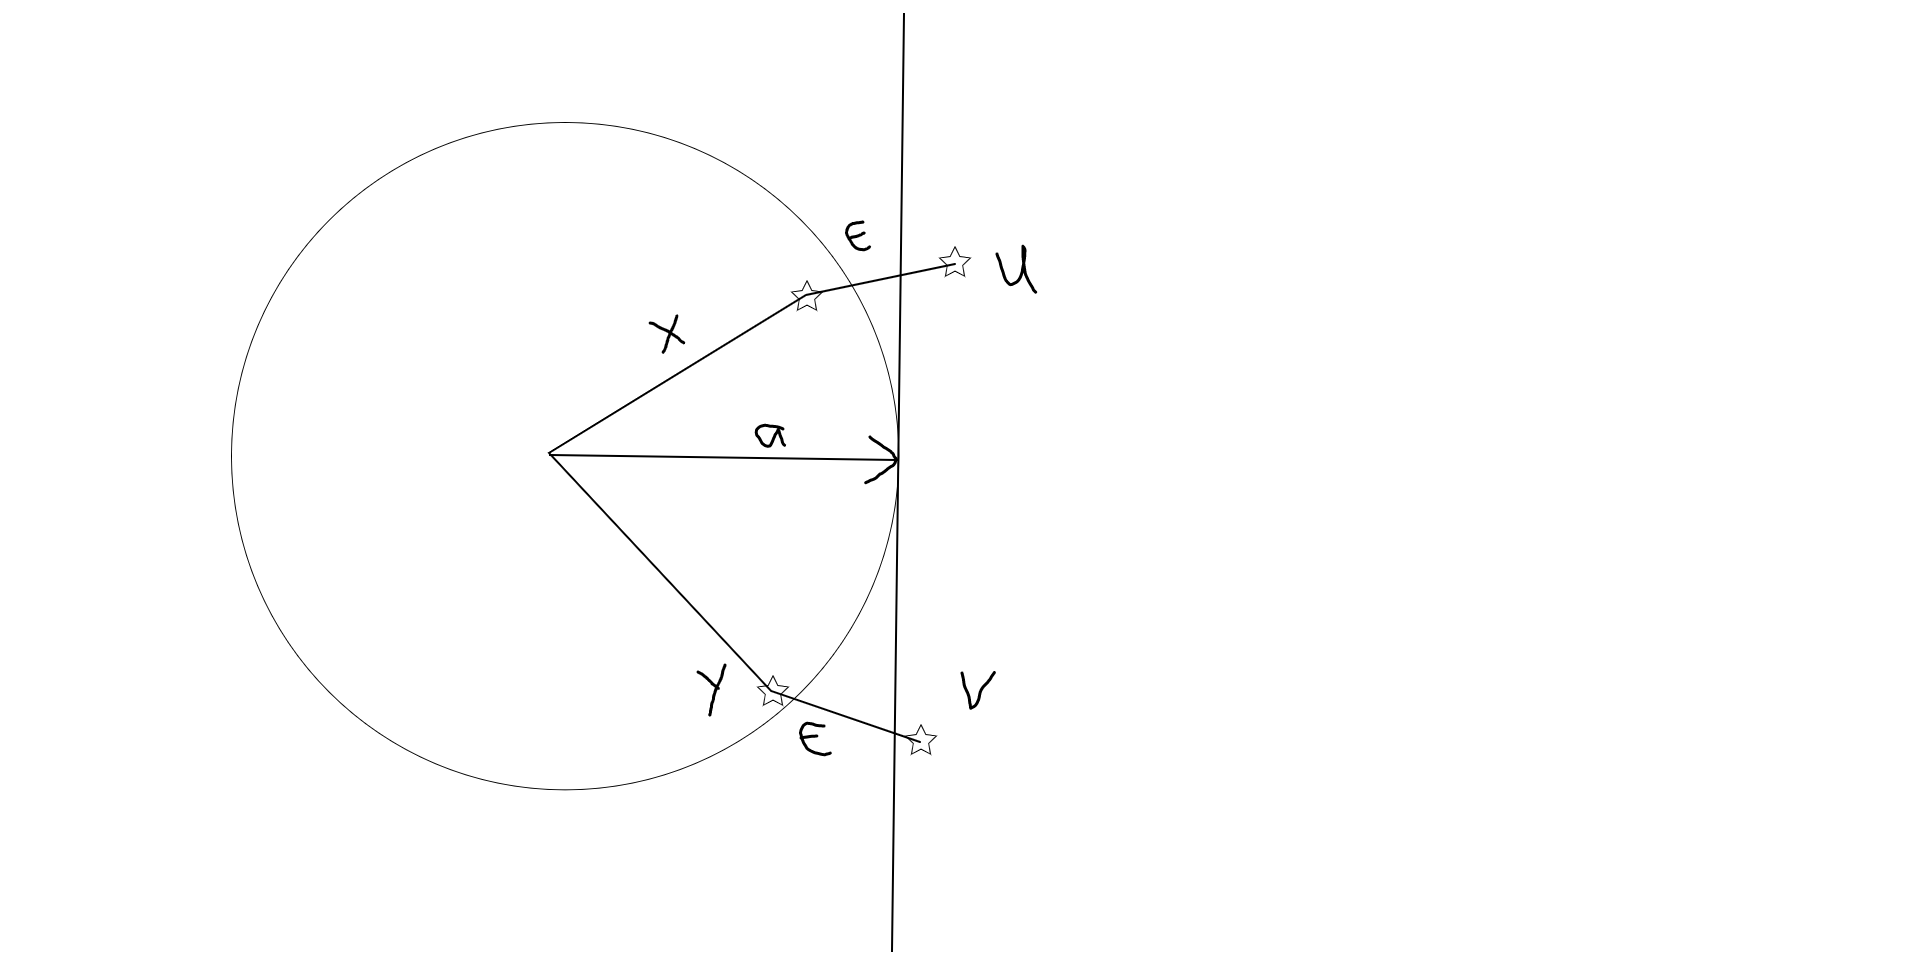
\includegraphics[width=300px]{images/first_lemma.png}
	\caption[
    		A depiction of the quantities within \cref{properties_of_a_circle}.]{
			The distances from $u$, $v$ to $x$, $y$ are less than $\epsilon$ respectively, and $x$ and $y$ lie within a sphere of radius $\|a\|$.
			Also, $a^Tx \le a^Ta$ separates the sphere from $u$ and $v$.
	}
	\label{first_lemma}
\end{figure}
The following lemma is illustrated in \cref{first_lemma}.
\begin{lemma}
\label[lemma]{properties_of_a_circle}
Suppose that $x, y, u, v, a \in \Rn$ and $0 < \epsilon \le 1$ are given satisfying
\begin{align*}
\|x\| \le \|a\|, \quad
\|y \| \le \|a\|, \quad
\|x - u \| \le \epsilon, \quad
\|y - v \| \le \epsilon, \quad
a^T u \ge a^T a, \quad
a^T v \ge a^T a.
\end{align*}
Then
\begin{align*}
\|x - y\| \le 8(1 + \|a\|) \sqrt{\epsilon}.
\end{align*}
\end{lemma}
\begin{proof}
If $\|a\| = 0$, then $x = y = 0$ so that $\|x - y\| = 0$.
We may now assume that $a \ne 0$.
We can combine
$
a^Tx  \le \|a\| \|x\| \le \|a\|^2 = a^T a
% a^Ty  \le \|a\| \|y\| \le \|a\|^2 = a^T a
$
with
$
a^Tx = a^T(x - u) + a^T u \ge a^Ta - \|a\| \epsilon
% a^Ty = a^T(y - v) + a^T v \ge a^Ta - \|a\| \epsilon
$
to see
$
a^Ta - \|a\|\epsilon \le a^Tx \le a^Ta \Longrightarrow 0 \le a^Ta - a^Tx \le \|a\| \epsilon.
% a^Ta - \|a\|\epsilon \le a^Ty \le a^Ta \Longleftrightarrow 0 \le a^Ta - a^Ty \le \|a\| \epsilon 
$
By symmetry, $0 \le a^Ta - a^Ty \le \|a\| \epsilon$ so that
\begin{align*}
\left| a^Tx - a^Ty \right| \le \|a\|\epsilon.
\end{align*}


% 
% \begin{align*}
% \left(a^Ta - a^Tx\right)^2 \le \|a\|^2 \epsilon
% \end{align*}
% 
% \begin{align*}
% \end{align*}

Considering this identity further, we see
$
a^Ta - \|a\| \epsilon \le a^Tx \le \|a\|\|x\| 
\Longrightarrow \|a\| - \epsilon \le  \frac{a}{\|a\|}^T x \le \|x\| 
\Longrightarrow -\|a\| + \epsilon \ge  -\frac{a}{\|a\|}^T x \ge -\|x\| 
\Longrightarrow 0 \le \|x\| -\frac{a}{\|a\|}^T x \le \|x\|-\|a\| + \epsilon \le \epsilon
$
and
$
|\|x\| + \frac{a}{\|a\|}^T x| \le \|x - \frac{a}{\|a\|}^T x\| + 2|\frac{a}{\|a\|}^T x| \le \epsilon + 2\|x\| \le 2\|a\| + \epsilon
$.
We multiply these to find
\begin{align*}
\sqrt{\|x\|^2 - \frac{\left(a^Tx\right)^2}{a^Ta}}
= \sqrt{\left(\|x\| - \frac{a}{\|a\|}^Tx\right)\left(\|x\| + \frac{a}{\|a\|}^Tx\right)} \\
\le \sqrt{2\|a\|\epsilon + \epsilon^2} \le \epsilon + \sqrt{2\|a\|\epsilon}.
\end{align*}



% Also, we see
% $
% 0 \le \left\|a - x\right\|^2 
% = \|a\|^2 + \|x\|^2 - 2a^Tx 
% \le \|a\|^2 + \|x\|^2 - 2\left(a^Ta - \|a\|\epsilon\right)
% = \|x\|^2 - \|a\|^2 + 2\|a\|\epsilon
% $
% so that
% $
% \|a\|^2 - 2\|a\|\epsilon \le \|x\|^2 \le \|a\|^2
% \Longrightarrow 0 \le \|a\|^2 - \|x\|^2 \le 2\|a\|\epsilon.
% $
% By symmetry,
% $
% 0 \le \|a\|^2 - \|y\|^2 \le 2\|a\|\epsilon
% $
% and we see
% \begin{align*}
% \left|\|x\|^2 - \|y\|^2\right| \le 2 \|a\|\epsilon.
% \end{align*}

Because
$
\left(x - \frac{a^Tx}{a^Ta} a\right)^T \frac{a^Tx}{a^Ta} a = \frac{a^Tx}{a^Ta} a^Tx - \left(\frac{a^Tx}{a^Ta}\right)^2a^Ta = 0,
$
% \left(y - \frac{a^Ty}{a^Ta} a\right)^T \frac{a^Ty}{a^Ta} a = \frac{a^Ty}{a^Ta} a^Ty - \left(\frac{a^Ty}{a^Ta}\right)^2a^Ta = 0 \\
we can compute
$
\|x\|^2 = \left\|x - \frac{a^Tx}{a^Ta} a + \frac{a^Tx}{a^Ta} a\right\|^2 = \left\|x - \frac{a^Tx}{a^Ta} a \right\|^2 +\frac{\left|a^Tx\right|^2}{a^Ta}
$
% \|y\|^2 = \left\|y - \frac{a^Ty}{a^Ta} a + \frac{a^Ty}{a^Ta} a\right\|^2 = \left\|y - \frac{a^Ty}{a^Ta} a \right\|^2 +\left|a^Ty\right|^2
so that 
$
\left\|x - \frac{a^Tx}{a^Ta} a \right\| = \sqrt{\|x\|^2 - \frac{\left|a^Tx\right|^2}{a^Ta}}.
$
%  \left\|y - \frac{a^Ty}{a^Ta} a \right\| = \sqrt{\|y\|^2 - \left|a^Ty\right|^2}
By symmetry,
$
\left\|y - \frac{a^Ty}{a^Ta} a \right\| = \sqrt{\|y\|^2 - \frac{\left|a^Ty\right|^2}{a^Ta}},
$
so that

\begin{align*}
\left\|x - \frac{a^Tx}{a^Ta} a - y + \frac{a^Ty}{a^Ta} a \right\|
\le \left\|x - \frac{a^Tx}{a^Ta} a \right\| + \left\|y - \frac{a^Ty}{a^Ta} a \right\|
\le 2\epsilon + 2\sqrt{2\|a\|\epsilon}.
\end{align*}

% \begin{align*}
% \left\|x - \frac{a^Tx}{a^Ta} a \right\|^2 - \left\|y - \frac{a^Ty}{a^Ta} a \right\|^2
% = \|x\|^2 - \|y\|^2 + \left(-\left|a^Tx\right|^2 + \left|a^Ty\right|^2\right) \\
% \left|\left\|x - \frac{a^Tx}{a^Ta} a \right\|^2 - \left\|y - \frac{a^Ty}{a^Ta} a \right\|^2\right|
% \le \left|\|x\|^2 - \|y\|^2\right| + \left|\left|a^Tx\right|^2 - \left|a^Ty\right|^2\right| \\
% \le 2 \|a\|\epsilon + 2 |a^Tx| \|a\|\epsilon + \|a\|^2\epsilon^2 \\
% \Longrightarrow 
% \left|\left\|x - \frac{a^Tx}{a^Ta} a \right\| - \left\|y - \frac{a^Ty}{a^Ta} a \right\|\right|
% \le \sqrt{2 \|a\|\epsilon + 2 |a^Tx| \|a\|\epsilon + \|a\|^2\epsilon^2}
% \le \|a\|\epsilon + \sqrt{2 \|a\|\epsilon\left(1 + |a^Tx|\right)}
% \end{align*}


% \begin{align*}
% \left\|x - \frac{a^Tx}{a^Ta} a - \left(y - \frac{a^Ty}{a^Ta} a\right)\right\|^2
% = \left\|x - \frac{a^Tx}{a^Ta} a\right\|^2 + \left\|y - \frac{a^Ty}{a^Ta} a\right\|^2 - 2\left(x - \frac{a^Tx}{a^Ta} a\right)^T\left(y - \frac{a^Ty}{a^Ta} a\right) \\
% = \left\|x - \frac{a^Tx}{a^Ta} a\right\|^2 + \left\|y - \frac{a^Ty}{a^Ta} a\right\|^2 - 2\left(x^Ty - \frac{a^Tya^Tx}{a^Ta}\right) \\
% \end{align*}
% 
% \begin{align*}
% \left\|x - \frac{a^Tx}{a^Ta} a - \left(y - \frac{a^Ty}{a^Ta} a\right)\right\|^2
% = \left\|x - \frac{a^Tx}{a^Ta} a\right\|^2 + \left\|y - \frac{a^Ty}{a^Ta} a\right\|^2 - 2\left(x - \frac{a^Tx}{a^Ta} a\right)^T\left(y - \frac{a^Ty}{a^Ta} a\right) \\
% = \left\|x - \frac{a^Tx}{a^Ta} a\right\|^2 + \left\|y - \frac{a^Ty}{a^Ta} a\right\|^2 - 2\left(x^Ty - \frac{a^Tya^Tx}{a^Ta}\right) \\
% \end{align*}



Finally, we combine everything to see
\begin{align*}
\|x - y\| 
\le \left\|x - \frac{a^Tx}{a^Ta} a - \left(y - \frac{a^Ty}{a^Ta} a\right)\right\| + |a^Tx - a^Ty|
\le (2 + \|a\|)\epsilon + 2\sqrt{2\|a\|\epsilon} \\
\le \left(2 + 2\sqrt{2\|a\|} + \|a\|\right)\sqrt{\epsilon}
\le \left(\sqrt{2} + \sqrt{\|a\|}\right)^2 \sqrt{\epsilon}
\le \left(2\max\{\sqrt{2},\sqrt{\|a\|}\}\right)^2 \sqrt{\epsilon} \\
\le 4\max\{2,\|a\|\} \sqrt{\epsilon}
\le 8\max\{1,\|a\|\} \sqrt{\epsilon}
\le 8(1 + \|a\|) \sqrt{\epsilon}
\end{align*}
% is small.
% = \epsilon \|a\| \left(2 + 2|a^Tx| + \|a\|\epsilon\right) \\

% \begin{align*}
% \left\|x - \frac{a^Tx}{a^Ta} a \right\| - \left\|y - \frac{a^Ty}{a^Ta} a \right\|
% = \sqrt{\|x\|^2 - \|y\|^2} - \sqrt{\left|a^Tx\right|^2 + \left|a^Ty\right|^2}
% \end{align*}

% \begin{align*}
% |x - y| \le \epsilon \\
% \Longleftrightarrow x - \epsilon \le y \le x + \epsilon \\
% \Longleftrightarrow x^2 - 2x\epsilon - \epsilon^2 \le x^2 - 2x\epsilon + \epsilon^2 \le y^2 \le x^2 + 2x\epsilon + \epsilon^2 \\
% \Longleftrightarrow  |x^2 - y^2| \le 2 x \epsilon + \epsilon^2
% \end{align*}
% 
% \begin{align*}
% \epsilon \le x^2 \\
% \Longrightarrow \sqrt{\epsilon} \le x \\
% \Longrightarrow 2\epsilon \le 2x\sqrt{\epsilon} \\
% \Longrightarrow x^2 - 2x\sqrt{\epsilon} + \epsilon \le x^2 - \epsilon \\
% \Longrightarrow x - \sqrt{\epsilon} \le \sqrt{x^2 - \epsilon}
% \end{align*}
% 
% \begin{align*}
% \left|x^2 - y^2\right| \le \epsilon \\
% \Longleftrightarrow x^2 - \epsilon \le y^2 \le x^2 + \epsilon \\
% \Longleftrightarrow x - \sqrt{\epsilon} \le \sqrt{x^2 - \epsilon} \le y \le \sqrt{x^2 + \epsilon} \le x + \sqrt{\epsilon} \\
% \Longleftrightarrow |x - y| \le \sqrt{\epsilon}
% \end{align*}

% \begin{align*}
% x^Tx \ge \frac{\|x\|}{\|a\|} a^T x
% \ge \frac{\|x\|}{\|a\|}\left(a^Ta - \|a\|\epsilon\right)
% \ge \|x\|\|a\| - \|x\| \epsilon 
% \ge \|x\|\left(\|a\| - \epsilon\right)
% \end{align*}
% 
% \begin{align*}
% x = x - \frac{a^Tx}{a^Ta} a + \frac{a^Tx}{a^Ta} a \\
% y = y - \frac{a^Ty}{a^Ta} a + \frac{a^Ty}{a^Ta} a
% \end{align*}
% 
% \begin{align*}
% \|x - y\| =
% \left\| x - \frac{a^Tx}{a^Ta} a  \right\|
% \end{align*}

\end{proof}


We define the distance from a point $s$ to a convex set $S$ as
\begin{align*}
D\left(s, S\right) = \inf_{s' \in S} \left\|s - s'\right\|,
\end{align*}
and the distance between any two convex sets $S_1$ and $S_2$ as
% \convexdistance\left(S_1, S_2\right) = \max_{s' \in S_1 \cup S_2} \min_{s \in S_1 \cap S_2} \|s' - s\|. \label{define_a_difference_between_sets}
\begin{align}
\convexdistance\left(S_1, S_2\right) = 
\max \left\{
	\sup_{s  \in S_1} D\left(s , S_2\right),
	\sup_{s' \in S_2} D\left(s', S_1\right)
\right\}. \label{define_a_difference_between_sets}
\end{align}
Note that $D\left(S_1, S_2\right) \ge 0$ for any two convex sets $S_1$, and $S_2$.


\begin{boxedcomment}
Not supposed to worry about $S \cap S' = \emptyset$.
\end{boxedcomment}

\begin{lemma}
\label[lemma]{board_tied_to_sphere}
Let $\convexdistance$ be defined by \cref{define_a_difference_between_sets}.

Let $g \in \Rn$ and let $S, S' \subseteq \Rn$ be convex with $S \cap S' \ne \emptyset$.
If $D\left(S, S'\right) \le 1$, then 
% Suppose that $0 < \epsilon \le 1$, then
% is given with $D\left(S, S'\right) \le \epsilon$.
% Then 
\begin{align*}
\|P_{S}(g) - P_{S'}(g)\| \le 8\left(1 + \|P_{S \cap S'}(g) - g\|\right) \sqrt{\convexdistance\left(S, S'\right)}.
\end{align*}
\end{lemma}
\begin{proof}
% Because $\convexdistance(S, S') \le \epsilon$, we know that $S \cap S' \ne \emptyset$.

% If $S \cap S' = \emptyset$, then $P_{S \cap S'}\left(g\right) = \infty$.

If $g \in S \cap S'$, then $\left\|P_S(g) - P_{S'}(g)\right\| = 0 \le 8\left(1 + \|P_{S \cap S'}(g) - g\|\right) \sqrt{\convexdistance\left(S, S'\right)}$.
Likewise, the left hand side is $0$ whenever $S = S'$.
Otherwise, $\convexdistance\left(S, S'\right) > 0$, and let 
\begin{align*}
\begin{array}{ccc}
x = P_S(g) - g      & u = P_{S \cap S'}(g + x) - g & a = P_{S \cap S'}(g) - g \\
y = P_{S'}(g) - g   & v = P_{S \cap S'}(g + y) - g. &  \\
\end{array}
\end{align*}
Because $S \cap S' \subseteq S$ and $S \cap S' \subseteq S'$ we have
$\|x\| = \|P_S(g) - g\| \le \|P_{S \cap S'} (g) - g\| = \|a\|$ and $\|y\| \le \|a\|$.
Also, because $S \cap S'$ is convex, the optimality conditions for $a$ imply the plane $a^Tx \ge a^Ta$ separates $S \cap S'$ from $g$.
In particular, $a^Tu \ge a^Ta$ and $a^Tv \ge a^Ta$.
Finally, by letting $0 < \epsilon = \convexdistance(S, S') \le 1$, we have $\|x - u\| = \|P_{S \cap S'}\left(P_S(g)\right)\| \le \epsilon$ and $\|y - v\| \le \epsilon$.
Thus, \cref{properties_of_a_circle} informs us
$\|P_S(g) - P_{S'}(g)\| = \|x - y\| \le 8(1 + \|a\|) \sqrt{\epsilon}$.
\end{proof}


\begin{corollary}
Let $\convexdistance$ be defined by \cref{define_a_difference_between_sets}.

Let $g, g' \in \Rn$ and let $S, S' \subseteq \Rn$ be convex with $S \cap S' \ne \emptyset$.
Suppose that $0 < \epsilon \le 1$ is given with $D\left(S, S'\right) \le \epsilon$ and $\|g - g'\| \le \epsilon$.
Then $\|P_S(g) - P_{S'}(g')\| \le 9\left(1 + \|P_{S \cap S'}(g) - g\|\right) \sqrt{\epsilon}$.
\end{corollary}
\begin{proof}
Notice
\begin{align*}
\|P_S(g) - P_{S'}(g')\| 
\le \|P_S(g) - P_{S'}(g)\| + \|P_{S'}(g) - P_{S'}(g')\| \\
\le \|P_S(g) - P_{S'}(g)\| + \|g - g'\| \\
\le 8\left(1 + \|P_{S \cap S'}(g) - g\|\right) \sqrt{\epsilon} + \epsilon \\
\le 9\left(1 + \|P_{S \cap S'}(g) - g\|\right) \sqrt{\epsilon}.
\end{align*}
\end{proof}

\begin{lemma}
\label[lemma]{the_lemma_to_end_all_lemmas}
Let $\convexdistance$ be defined by \cref{define_a_difference_between_sets}.

Let
$A, A' \in \mathbb \mathbb R^{m \times n}$;
$b, b' \in \mathbb \mathbb R^{m}_{\ge 0}$;
$C, C' \in \mathbb \mathbb R^{m' \times n}$;
$d, d' \in \mathbb \mathbb R^{m'}_{\ge 0}$;
unit vector $u \in \Rn$;
and constants
$\delta_l$,
$\delta_u$,
$\delta_r$,
$\delta_{\alpha} > 0$
be given such that
\begin{align*}
\begin{array}{cccc}
\delta_r \|A_i\| \le b_i,			&
Cu \ge \delta_{\alpha} e,			&
\delta_l \le \|A_i\| \le \delta_u	\\
\delta_r \|A_i'\| \le b_i',			&
C'u \ge \delta_{\alpha} e, 			&
\delta_l \le \|A'_i\| \le \delta_u.
\end{array}
\end{align*}
% be given such that $\left\|A_i\right\| > 0$ and $\left\|A'_i\right\| > 0$ for all $i \in [m]$.
% Suppose there exists a unit vector $u \in \Rn$ with $Cu > 0$ and $C'u > 0$.
Given $p \in \Rn$ and $r > 0$, define the sets
\begin{align*}
\begin{array}{ccccc}
S  &= \bigg\{x \in \Rn \bigg|& A (x - p) \le b ,& C (x - p) \le d ,& \|x - p\| \le r \bigg\}, \\
S' &= \bigg\{x \in \Rn \bigg|& A'(x - p) \le b',& C'(x - p) \le d',& \|x - p\| \le r \bigg\}.
\end{array}
\end{align*}
and for any $0 < \epsilon < r$, define the constants
\begin{align*}
\begin{array}{cccccc}
\lambda &=& \delta_{\alpha}^{-1}(r + 1) (\delta_u + 2), &
\gamma &=& 2\lambda(\delta_r \delta_u)^{-1}, \\
\eta    &=& \frac 1 2 \epsilon\delta_{\alpha}(r+2)^{-1}(r + 1)^{-1}, &
\delta &=& \min\bigg\{
1,
\gamma^{-1},
\frac 1 2 {\epsilon} (\gamma r)^{-1},
\eta
\bigg\}.
\end{array}
\end{align*}
If
\begin{align*}
\begin{array}{ccccc}
\|A - A'\|_{\infty} \le \delta,	& \|b - b'\|_{\infty} \le \delta,		& \|C - C'\|_{\infty} \le \delta,	& \textrm{and} & \|d - d'\|_{\infty} \le \delta
\end{array},
\end{align*}
then
$D(S, S') \le \epsilon$.



% \delta_1 \le \delta_2 \|A_i\| \le b_i, 
% \delta_1 \le \delta_2 \|A'_i\| \le b'_i, \\
% \gamma = \frac{2}{\delta_1}\left(1 + \|y\|\right), 
% \epsilon \le \min\left\{\gamma^{-1}\right\}.


\end{lemma}
% y - z  =       A        ^T\mu  + C^T\lambda  \\
% y - z' = \left(A'\right)^T\mu' + C^T\lambda' \\
% t &=  \max_{\substack{i \in [m] \\ A'_i(z - p) > b'_i}} \frac{A'_i (z - p) - b'_i}{A'_i (z - p)} \\

\begin{proof}
% (1 + r)\left[1 + \delta_{\alpha}^{-1} \left(\delta_2 + 1\right)\right]
\begin{boxedcomment}
No longer usable:
Define
\begin{align*}
\begin{array}{cccccc}
\delta_l &=& \min_{1\le i\le m} \min\left\{ \left\|A_i\right\|, \left\|A'_i\right\| \right\},  &
\delta_u &=& \max_{1\le i\le m} \max\left\{ \left\|A_i\right\|, \left\|A'_i\right\| \right\}, \\
\delta_r &=& \min_{1\le i\le m} \min\left\{ \frac{b_i}{\left\|A_i\right\|}, \frac{b_i}{\left\|A'_i\right\|} \right\}, &
\textrm{and} \quad \delta_{\alpha} &=& \max \left\{ \left\|Cu\right\|_{\infty}, \left\|C'u\right\|_{\infty} \right\},
\end{array}
\end{align*}
so that
\begin{align*}
\begin{array}{cccc}
\delta_r \|A_i\| \le b_i,			&
Cu \ge \delta_{\alpha} e,			&
\delta_l \le \|A_i\| \le \delta_u	\\
\delta_r \|A_i'\| \le b_i',			&
C'u \ge \delta_{\alpha} e, 			&
\delta_l \le \|A'_i\| \le \delta_u.
\end{array}
\end{align*}
\end{boxedcomment}

Let $x \in S$, and define
\begin{align*}
\begin{array}{cccccc}
s &=& \delta(r + 1)\delta_{\alpha}^{-1}, &
z &=& x - su, \\
t &=& \max\left\{\gamma \delta, s(r+s)^{-1}\right\}, &
v &=& (1-t)z + t p.
\end{array}
\end{align*}
The construction of $v$ has the following intuition:
to travel to $v$ from $x$, we
\begin{itemize}
\item first travel a distance $s$ along $-u$ to reach $z$ (where we will show $C'(z-p) \le d'$),
\item then travel a fraction $t$ of the distance back to $p$ (where both $A'(v - p) \le b'$ and $\|v-p\| \le r$).
\end{itemize}
Throughout the remainder of this proof, we will show $v \in S'$ and $\|x - v\| \le \epsilon$.
The result then follows from the symmetry of $S$ and $S'$.


For each $i \in [m]$,
\begin{align*}
0 \le C_i'(x-p) - d_i'
\le C_i(x - p) - d_i + (C_i' - C_i)(x-p) + d_i - d_i'  \\
\le 0 + \|C_i' - C_i\| \|x - p\| + \|d_i - d_i'\| 
\le \delta (r+1)
= \delta_{\alpha} s \le sC_i'u
\end{align*}
so that
\begin{align}
-sC_i'u \le d_i' - C_i'(x - p) \Longrightarrow C'(z - p) = C'(x - su - p) \le d'. \label{reun_eqn3}
\end{align}

\begin{boxedcomment}
Explanation for next sentence:
\begin{align*}
s\delta_u + \delta \left(s + r\right) + \delta 
&= \frac{\delta(r + 1)}{\delta_{\alpha}}\delta_u + \delta \left(s + r\right) + \delta \\
&\le \delta \left[(r + 1)\frac{\delta_u}{\delta_{\alpha}} + (r+1)\frac{\delta}{\delta_{\alpha}} + r + 1\right] \\
&\le \delta (r + 1) \left[\frac{\delta_u}{\delta_{\alpha}} + \frac{\delta}{\delta_{\alpha}} + 1\right] \\
&\le \delta (r + 1) \left[\frac{\delta_u}{\delta_{\alpha}} + \frac{1}{\delta_{\alpha}} + \frac{1}{\delta_{\alpha}}\right] \\
&\le \delta \delta_{\alpha}^{-1}(r + 1) (\delta_u + 2)
\end{align*}
\end{boxedcomment}
Also, without loss of generality, $\delta_{\alpha} \le 1$, so that
\begin{align}
A_i'(z - p) - b_i' 
&= - s A_iu + A_i(x - p) - b_i + (A_i' - A_i)(z - x + x - p) + (b_i' - b_i) \nonumber \\
&\le s \|A_i\|\|u\| + 0 + \|A_i' - A_i\|\left[\|z - x\| + \|x - p\|\right] + \|b_i'-b_i\| \nonumber \\
&\le s\delta_u + \delta \left(s + r\right) + \delta \le \lambda \delta \label{reun_eqn1}
\end{align}
so that whenever $A_i'(z - p) > b_i'$,
\begin{align}
\left|A_i'(z - p)\right| 
\ge |b_i'| - \left| A_i'(z - p) - b_i'\right| 
\ge \delta_r\|A_i'\| - \lambda \delta 
\ge \delta_r \delta_u - \lambda \delta \ge \frac 1 2 \delta_r \delta_u. \label{reun_eqn2}
\end{align}
% \Longrightarrow \frac 1 {\left|A_i'(z - p)\right|} \le \frac 2 {\delta_1 \delta_3}. 

% &= A_i(z - p) - b_i + (A_i' - A_i)(z - p) + (b_i' - b_i) \\
% \begin{align*}
% A_i(z - p) - b_i = A_i(x - p) - b_i - s A_iu \le 0 + s \|A_i\| \|u\| \le s\delta_2
% \end{align*}
% so that

% \begin{align*}
% \lambda \delta \le \frac 1 2 \delta_1 \delta_3
% \end{align*}
% \begin{align*}
% (1 - t) A_i'\left[z - p\right] \le b_i' \\
% A_i'\left[(1-t) z + tp - p\right] \le b_i'
% \end{align*}

Dividing \cref{reun_eqn1} by \cref{reun_eqn2}, we find
\begin{align*}
\frac{A'_i (z - p) - b'_i}{A'_i (z - p)} \le \frac{2\lambda}{\delta_r \delta_u}\delta = \gamma \delta \le 1
\end{align*}
which means $t = \max\left\{\gamma \delta, \frac{s}{r+s}\right\} \in [0, 1]$.
Also, note that for each $i \in [m]$, if $A_i'(z - p) > b_i'$, then
\begin{align*}
t \ge \frac{A'_i (z - p) - b'_i}{A'_i (z - p)}
\Longrightarrow (1-t) A'_i (z - p) \le b'_i.
\end{align*}
But if $A_i'(z - p) \le b_i'$, then $t \le 1$ and $b_i' \ge 0$ provide the same identity.
Therefore, 
\begin{align*}
A'(v - p) = A' \bigg[(1-t) z + tp - p\bigg] = (1-t) A' (z - p) \le b'.
\end{align*}
Because $t \in [0, 1]$, \cref{reun_eqn3} and convexity imply $C'(v - p) \le d$.
Lastly, $t \ge \frac{s}{r + s} \Longrightarrow (1 - t) \left(r + s\right) \le r$, so that
\begin{align*}
\|v - p\| 
= \|(1-t)z + t p - p\| 
= (1 - t) \|z - p\| \\
\le (1 - t) \left(\|x - p\| + s\right) 
\le (1 - t) \left(r + s\right) 
\le r
\end{align*}
and $v \in S'$.
\begin{boxedcomment}
Explanation:
\begin{align*}
t \ge \frac{s}{r + s} \\
 tr + ts \ge s \\
- tr - ts \le -s \\
r - tr + s - ts \le r \\
(1 - t) r + (1 - t)s \le r \\
(1 - t) \left(r + s\right) \le r \\
\end{align*}
\end{boxedcomment}

Finally, we will show $\|v - x\| \le \epsilon$.
Notice that $\delta \le \eta = \frac{\epsilon\delta_{\alpha}}{2(r+2)(r + 1)} \Longrightarrow s \le \frac{\epsilon}{4 + 2r - \epsilon}$, which implies two things.
First, it means $s \le \frac{\epsilon}{2r - \epsilon}$ so that
$\frac {s}{1 + s} \le \frac {\epsilon} {2r}. $
Combine this with $\delta \le \frac {\epsilon} {2\gamma r}$ to find that $tr \le \frac 1 2 \epsilon$.
Secondly, it means that
$s \le \frac{\epsilon}{4}$ so that $(1 + t)s \le \frac 1 2 \epsilon$.
Combining these produces,
\begin{align*}
\|x - v\| 
\le \|x - z\| - \|z - v\| 
= s + t \|p - z\| 
\le s + t \left(r + s\right) 
= (1 + t)s + tr \\
\le \frac 1 2 \epsilon + \frac 1 2 \epsilon = \epsilon.
\end{align*}
% = s + \|(1-t) z + tp - z\| 

\begin{boxedcomment}
Explanations:
\begin{align*}
\delta \le \frac{\epsilon\delta_{\alpha}}{2(r+2)(r + 1)}
\le \frac{\epsilon\delta_{\alpha}}{(4 + 2r - \epsilon)(r + 1)} \\
\Longrightarrow \frac{\delta(r + 1)}{\delta_{\alpha}}  \le \frac{\epsilon}{4 + 2r - \epsilon} 
\Longrightarrow s\le \frac{\epsilon}{4 + 2r - \epsilon}
\end{align*}
\begin{align*}
s\le \frac{\epsilon}{(2r - \epsilon)} \Longrightarrow
s(2r - \epsilon)\le \epsilon \Longrightarrow
2rs \le \epsilon(1 + s) \Longrightarrow
\frac {s}{1 + s} \le \frac {\epsilon} {2r}
\end{align*}
\begin{align*}
s \le \frac{\epsilon}{4 + 2r - \epsilon} \le \frac 1 4 \epsilon \Longrightarrow
(1 + t)s \le 2s \le \frac 1 2 \epsilon
\end{align*}
\end{boxedcomment}
\end{proof}

\subsubsection{Simplifed Results}
\label{simplifed_bounded_projection}



% We prove the convergence results found within \cref{limit_of_true_criticallity} by contradiction.
% Namely, we assume the existence of an $\epsilon_{\textrm{lb}} > 0$ within \cref{the_contradiction}, 
% and within \cref{lim_chi_to_zero}, we show that $\epsilon_{\textrm{lb}}$ cannot exist.
% To accomplish this, we define a certain set of pairs of iterates within \cref{define_slb}.
% We generalize this set within following definition.

% \begin{definition}
% \label{criteria_from_contradiction}
% A sequence $S \subseteq\naturals \times \naturals$ satisfies this definition if
% is called a \emph{Cauchy pair-subsequence} if
% Let $l, k \in S \subseteq \naturals$, where $S$ is such that the subsequence $\{\xk\}_{k \in S}$ is Cauchy.
% for any $\epsilon > 0$, there exists $k_0 \in \naturals$ such that if $(k, l) \in S$ with $k, l \ge k_0$, 
% then 
% $\left\|\xk - \xl \right\| \le \epsilon$.
% There exists $x^{\star}$ such that $\lim_{k\to\infty} \xk = x^{\star}$.
% \end{definition}



\begin{lemma}
\label[lemma]{model_gradients_are_cauchy}
Let $\ulb$ and $\slb$, be defined by \cref{define_the_finite_set} and \cref{define_slb}.

Suppose that \cref{bounded_below_assumption}---\cref{minangleassumption_alt} and \cref{restorability_assumption} hold.


If there exists $\elb > 0$ such that $\ulb$ is infinite, 
then for each $i \in [m]$ and any $\epsilon > 0$, there is a $k_0 \in \naturals$
such that if $(k, l) \in \slb$ and $k, l \ge k_0$, then $\left\|\gmcik - \gmcil \right\| \le \epsilon$.
\end{lemma}
\begin{proof}
Let $\epsilon > 0$ be arbitrary.
By \cref{contradiction_portion}, we can choose $k_1 \in \naturals$ such that if $k, l \ge k_1$ and
$k, l \in \slb$ then $\lipgrad \left\|\xk - \xl \right\| \le \frac 1 3 \epsilon$.
By \cref{delta_to_zero}, we can choose an $k_2 \in \naturals$ such that $\kappa_g \dk^2 \le \frac 1 3 \epsilon $ whenever $k \ge k_2$.
Choose $k_0 = \max\{k_1, k_2\}$, and let $d, k \ge k_2$.
By the triangle inequality, \cref{accuracy_is_satisfied}, and \cref{lipschitz_gradients_assumption}:
\begin{align*}
\left\|\nabla \mcik\left(\xk\right) - \nabla \mcil\left(\xl\right) \right\| \\
\le 
\left\|\nabla \mcik\left(\xk\right) - \nabla c_i\left(\xk\right) \right\|
+ \left\|\nabla c_i\left(\xk\right) - \nabla c_i\left(\xl\right)\right\| \\
+ \left \| \nabla c_i\left(\xl\right) - \nabla \mcil\left(\xl\right) \right \| \\
\le \kappa_g \left(\dk^2 + \dl^2\right) + \lipgrad \left\|\xk - \xl \right\|
\le \frac 1 3 \epsilon + \frac 1 3 \epsilon + \frac 1 3 \epsilon = \epsilon.
\end{align*}
\end{proof}
% \left\|\mcik\left(\xk\right) - \mcik\left(\xl\right) \right\| + \left \| \mcik\left(\xl\right) - \mcil\left(\xl\right) \right\|





Let $\minangledelta$ be defined by \cref{minangleassumption_alt} and define
% such that if $\dk \le \minangledelta$ and
\begin{align}
\activeindicesk = \left\{i \in [m] \bigg| -c_i\left(\xk\right) \le \minangledelta \left\|\gmcik\right\| \right\}. \label{define_activeindicesk}
\end{align}


% \begin{align*}
% ? =  \\
% c_i\left(\xk\right) + \gmcik^T \gk
% \end{align*}

The following observation follows directly from the definition:
\begin{lemma}
\label[lemma]{doesntreallyneedtobesaid}
Let $\activeindicesk$, $\zik$, $\minangledelta$ be defined by \cref{define_activeindicesk}, \cref{define_z}, and \cref{minangleassumption_alt} respectively.

If $i \in \activeindicesk$, then $\zik \in B_{\infty}\left(\xk, \minangledelta \right)$.
\end{lemma}
\begin{proof}
If $c_i\left(\xk\right) = 0$, then $\zik = \xk \in B_{\infty}\left(\xk, \minangledelta \right)$.
Otherwise, $\left\|\gmcik\right\| \ge \frac{-c_i\left(\xk\right)}{\minangledelta} \ge 0$, so
\begin{align*}
\zik = \xk - \frac{m^{(k)}_{c_i}\left(\xk\right)}{\left\|\gmcik\right\|^2} \gmcik \\
\Longrightarrow \left\|\xk - \zik \right\|= -\frac{c_i\left(\xk\right)}{\left\|\gmcik\right\|} \le \minangledelta.
\end{align*}
\end{proof}

\begin{lemma}
\label[lemma]{underbound}
Let $\activeindicesk$ be defined by \cref{define_activeindicesk}, and $\mingradepsilon$ and $\mingrad$ be defined by \cref{mingradassumption}.

Suppose that \cref{mingradassumption} holds.


There exists $k_0 \in \naturals$ such that if $k \ge k_0$, then
for all $i \in \activeindicesk$,
\begin{align*}
\left\|\gmcik\right\| \ge \activegradmin
\end{align*}
where
\begin{align}
\label{define_activegradmin}
\activegradmin = \min\left\{\mingrad, \frac{\mingradepsilon}{\sqrt{n} \minangledelta}\right\}.
\end{align}
\end{lemma}
\begin{proof}

By \cref{mingradassumption}, if $-c_i\left(\xk\right) \le \mingradepsilon$, then $\left\|\nabla c_i\left(\xk\right)\right\| \ge \mingrad \ge \activegradmin$.
On the other hand, if $-c_i\left(\xk\right) \ge \mingradepsilon$ and $i \in \activeindicesk$, by \cref{define_z}
\begin{align*}
\sqrt{n} \minangledelta \ge \left\|\xk - \zik \right\|
= \frac{-c_i\left(\xk\right)}{\left\|\gmcik\right\|}
\ge \frac{\mingradepsilon}{\left\|\gmcik\right\|} \\
\Longrightarrow
\left\|\gmcik\right\| \ge \frac{\mingradepsilon}{\sqrt{n} \minangledelta} \ge \activegradmin.
\end{align*}
\end{proof}


\begin{lemma}
\label[lemma]{yet_another_bound_on_a_u}

Let $\ulb$, $\slb$, and $\activeindicesk$ be defined by \cref{define_the_finite_set}, \cref{define_slb}, and \cref{define_activeindicesk} respectively.

Suppose that \cref{bounded_below_assumption}---\cref{mingradassumption} hold.


There exists $k_0 \in \naturals$, scalar $\minactivealpha > 0$, and unit vector $\activedirk \in \Rn$ such that if 
$k \ge k_0$, then $\forall i \in \activeindicesk$:
\begin{align*}
\gmcik^T \activedirk \ge \minactivealpha
\quad \textrm{and} \quad
\nabla c_i\left(\xk\right)^T \activedirk \ge \minactivealpha.
\end{align*}

Furthermore, if there is an $\elb > 0$ such that $\ulb$ is infinite, then for any $(k, l) \in \slb$, $k,l \ge k_0$, and $\forall i \in \activeindicesk$
\begin{align*}
\gmcil^T \activedirk \ge \minactivealpha.
\end{align*}
\end{lemma}
\begin{proof}

Let 
$\minanglealpha$ and $\minangledelta$ be defined by \cref{minangleassumption_alt};
$\kappa_g$ be defined by \cref{accuracy_is_satisfied}; 
and $\activegradmin$ be defined by \cref{define_activegradmin}.

Define 
\begin{align}
\minactivealpha = \frac 1 2 \minanglealpha \activegradmin. \label{define_minactivealpha}
\end{align}

By \cref{delta_to_zero}, we know there exists $k_1 \in \naturals$ such that if $k \ge k_1$, then
\begin{align*}
\dk \le \minangledelta \quad \textrm{and} \quad  \dk \le \sqrt{\frac {\minanglealpha \activegradmin} {2 \kappa_g}}.
\end{align*}
By \cref{doesntreallyneedtobesaid}, we have $\zik \in B_{\infty}\left(\xk, \minangledelta \right)$ for all $i \in \activeindicesk$.
Thus, \cref{minangleassumption_alt} provides a unit vector $\minangledirk\in\Rn$ such that
\begin{align*}
-\frac {\gmcik}{\left\|\gmcik\right\|} ^T\minangledirk \ge \minanglealpha.
\end{align*}
Combining this with \cref{underbound}, we see that there exists and $k_2 \in \naturals$ such that for all $i \in \mathbb I^{(k)}$, $k \ge k_2$:
\begin{align*}
 \gmcik^T\left(-\minangledirk\right) \ge \minanglealpha \activegradmin
\end{align*}
Also, by \cref{accuracy_is_satisfied}, we have
\begin{align*}
\left\|\gmcik - \nabla c_i\left(\xk\right) \right\| \le \kappa_g \dk^2 \le \frac 1 2 \minanglealpha \activegradmin
\end{align*}
so that
\begin{align*}
\nabla c_i\left(\xk\right)^T \left(-\minangledirk\right) \\
= \gmcik^T\left(-\minangledirk\right) + \left(\gmcik - \nabla c_i\left(\xk\right) \right)^T\left(-\minangledirk\right) \\
\ge \minanglealpha \activegradmin - \left\|\gmcik - \nabla c_i\left(\xk\right) \right\|\left\|\minangledirk\right\|
\ge \minanglealpha \activegradmin - \frac 1 2 \minanglealpha \activegradmin = \minactivealpha.
\end{align*}

Furthermore, if there is a $\elb > 0$ such that $\ulb$ is infinite,
then \cref{model_gradients_are_cauchy} provides a $k_3 \in \naturals$ such that if $(k, l) \in \slb$ and $k, l \ge k_3$
\begin{align*}
\left\|\gmcik - \gmcil\right\| \le \frac {\minanglealpha \activegradmin} {2}.
\end{align*}
Thus,
\begin{align*}
\left\|\gmcil \left(-\minangledirk\right) \right\| \\
= \left\|\gmcik^T\left(-\minangledirk\right) + \left(\gmcik - \gmcil \right)^T\left(-\minangledirk\right)\right\| \\
\ge \minanglealpha \activegradmin - \left\|\gmcik - \gmcil \right\|\left\|\minangledirk\right\|
\ge \minanglealpha \activegradmin - \frac {\minanglealpha \activegradmin} {2} = \minactivealpha.
\end{align*}
Thus, we must only set $k_0 = \max \left\{k_1, k_2, k_3\right\}$ and $\activedirk=-\minangledirk$.
\end{proof}




% 
% 
% 
% \begin{align*}
% \left\|z - p\right\| = r \\
% r \le \left\|z' - p\right\| = r + \epsilon \\
% (z - p)^T (z' - p) \ge \|z - p\|^2
% \end{align*}
% 
% \begin{align*}
% \left\|z - z'\right\|
% \end{align*}
% 
% 
% 


% \begin{lemma}
% aabbcc
% \end{lemma}
% \begin{proof}
% By the mean value theorem, there exists $t \in [0, 1]$ such that
% \begin{align*}
% \end{align*}
% \end{proof}

Define
\begin{align}
\truefeasiblek &= \left\{ x \in \Rn \bigg| c_i\left(\xk\right) + \nabla c_i\left(\xk\right)^T \left(x - \xk\right) \le 0 \; \forall i \in [m] \right\}. \label{define_truefeasiblek}
\end{align}

% \begin{boxedcomment}
% Use a superscript of $(k, l)$
% \end{boxedcomment}


% https://mirror.las.iastate.edu/tex-archive/info/symbols/comprehensive/symbols-a4.pdf#page=123

Let $\feasiblek$, $\truefeasiblek$ be defined by \cref{define_feasiblek} and \cref{define_truefeasiblek} respectively, 
and for any fixed $k$, define

% \Amk &= \left\{ i \in [m] \bigg | c_i\left(\xk\right) + \gmcik^T\left( P_{\feasiblek}\left(\xk - \gk\right) - \xk\right) = 0\right\}, \label{tbbt_a1} \\
\begin{align}
\Alk &= \left\{ i \in [m] \bigg | c_i\left(\xl\right) + \gmcil^T\left( P_{\feasiblel}\left(\xk - \gk\right) - \xl\right) = 0\right\}, \label{tbbt_a2} \\
\Ack &= \left\{ i \in [m] \bigg | c_i\left(\xk\right) + \nabla c\left(\xk\right)^T\left( P_{\truefeasiblek}\left(\xk - \gk\right) - \xk\right) = 0\right\}. \label{tbbt_a3}
\end{align}

\begin{lemma}
\label[lemma]{norm_of_active_constraints_bounded_below}
Let $\Alk$ and $\Ack$ be defined by \cref{tbbt_a2} and \cref{tbbt_a3}.
Let $\ulb$ and $\slb$, be defined by \cref{define_the_finite_set} and \cref{define_slb}.

Suppose that \cref{bounded_below_assumption}---\cref{mingradassumption} hold.


There exists $\deltalb > 0$ and $k_0 \in \naturals$ such that,
\begin{itemize}
\item if $k \ge k_0$ and $i \in \Amk \cup \Ack$, then
\begin{align*}
\left\|\gmcik\right\| \ge \deltalb \quad \textrm{and} \quad
\left\|\nabla c_i\left(\xk\right) \right\| \ge \deltalb.
\end{align*}
\item if there exists an $\elb > 0$ such that $\ulb$ is infinite
$k, l \ge k_0$, $(k, l) \in \slb$, and $i \in \Amk \cup \Alk$, then
\begin{align*}
\left\|\gmcil\right\| \ge \deltalb.
\end{align*}
\end{itemize}
\end{lemma}
\begin{proof}

Let $\mingradepsilon > 0$ and $\mingrad > 0$ be defined by \cref{mingradassumption}
and $\maxmodelgrad \ge 1$ be defined by \cref{i_thought_i_proved_this_already}.
% and $\maxgrad$ be defined by \cref{bounded_gradients_lemma}.
Define
\begin{align*}
\deltalb = \min\left\{\frac 1 3 \mingrad, \frac 1 {6} \frac{\mingradepsilon}{\maxmodelgrad} \right\}.
\end{align*}

Before going through several cases, we make four observations.
First, \cref{i_thought_i_proved_this_already} and \cref{delta_to_zero} imply the existence of $k_1 \in \naturals$
such that if $k \ge k_1$, then as $\xk \in \feasiblek$ which is convex,
\begin{align*}
\left\|P_{\feasiblek}\left(\xk - \gk\right) - \xk\right\| 
\le \left\|\xk - \gk - \xk \right\| \le \maxmodelgrad.
\end{align*}
Secondly, \cref{accuracy_is_satisfied} and \cref{delta_to_zero} imply the existence of $k_2 \in \naturals$ such that if $k \ge k_2$, then
\begin{align}
\left\|\gmcik - \nabla c_i\left(\xk\right)\right\| \le \kappa_g \dk^2 \le \deltalb. \label{hmoydihtp_eqn1}
\end{align}
Similarily, \cref{model_gradients_are_cauchy} implies the existence of $k_3 \in \naturals$ such that if $k, l \ge k_3$, then 
\begin{align}
\left\|\gmcik - \gmcil\right\| \le \deltalb. \label{hmoydihtp_eqn2}
\end{align}
% \min\left \{\frac 1 2 \mingrad, \deltalb \right\}
Lastly, by the mean value theorem, for each $i \in [m]$, there exists $t_i \in [0, 1]$ such that
\begin{align*}
c_i\left(\xl\right) = c_i\left(\xk\right) + \nabla c_i\left((1 - t_i)\xk + t_i \xl\right)^T\left(\xl - \xk\right).
\end{align*}
Thus, if $(k, l) \in \slb$, \cref{contradiction_portion} and \cref{bounded_gradients_lemma}
imply the existence of $\maxgrad > 0$ and $k_4 \in \naturals$ such that if $k, l \ge k_4$, 
then
\begin{align}
\left\|c_i\left(\xk\right) - c_i\left(\xl\right) \right\| \le \maxgrad \left\|\xl - \xk\right\| \le \deltalb. \label{hmoydihtp_eqn3}
\end{align}
We choose $k_0 = \max\left\{k_1, k_2, k_3, k_4\right\}$, and assume $k, l \ge k_0$.

\paragraph*{Case 1}
If $-c_i\left(\xl\right) \le \mingradepsilon$, then \cref{mingradassumption} implies $\left\| \nabla c_i\left(\xl\right) \right\| \ge \mingrad \ge 3 \deltalb$.

\paragraph*{Case 2}
Suppose that $-c_i\left(\xk\right) > \mingradepsilon$ and $i \in \Ack$.
Then
\begin{align*}
\left\|\nabla c_i\left(\xk\right)  \right\| \maxmodelgrad
\ge \nabla c_i\left(\xk\right) ^T\left(P_{\truefeasiblek}\left(\xk - \gk\right) - \xk\right) \\
= -c_i\left(\xk\right) > \mingradepsilon \ge 6 \deltalb \maxmodelgrad.
\end{align*}
and $\left\|\nabla c_i\left(\xk\right)  \right\| \ge 6 \deltalb$.

% (1 - x) = 4x

\paragraph*{Case 3}
Suppose that $-c_i\left(\xk\right) > \mingradepsilon$ and $i \in \Amk$.
Then
\begin{align*}
\left\|\gmcik\right\| \maxmodelgrad
\ge \gmcik^T\left[P_{\feasiblek}\left(\xk - \gk\right) - \xk\right] \\
= -c_i\left(\xk\right) > \mingradepsilon \ge 6 \deltalb \maxmodelgrad.
\end{align*}
so that $\left\|\gmcik\right\| \ge 6 \deltalb$, and \cref{hmoydihtp_eqn1} implies $\| \nabla c_i\left(\xl\right) \| \ge 5 \deltalb$.

\paragraph*{Case 4}
Suppose that $-c_i\left(\xk\right) > \mingradepsilon$ and $i \in \Alk$.
Then \cref{hmoydihtp_eqn3} implies that $-c_i\left(\xl\right) > \mingradepsilon - \deltalb \ge (6\maxmodelgrad - 1) \deltalb \ge 5 \deltalb$, so that
\begin{align*}
\left\|\gmcil\right\| \maxmodelgrad
\ge \gmcil^T\left(P_{\feasiblek}\left(\xl - \gk\right) - \xl\right) \\
= -c_i\left(\xl\right) > 5 \deltalb \maxmodelgrad.
\end{align*}
Hence, $\left\|\gmcil\right\| \ge 5 \deltalb$.
Then by \cref{hmoydihtp_eqn2}, $\left\|\gmcik\right\| \ge 4 \deltalb$, and by \cref{hmoydihtp_eqn1} $\left\|\nabla c_i\left(\xk\right) \right\| \ge 3 \deltalb$.


% Without loss of generality, we may assume that $\maxmodelgrad \ge 1$, so that 



Throughout the cases, we have established if $i \in \Amk \cup \Ack \cup \Alk$, then $\left\| \nabla c_i\left(\xk\right) \right\| \ge 3 \deltalb$.
Then \cref{hmoydihtp_eqn1} implies $\left\|\gmcik\right\| \ge 2 \deltalb$, 
and \cref{hmoydihtp_eqn2} implies $\left\|\gmcil\right\| \ge \deltalb$.
\end{proof}

% 
% 
% \begin{boxedcomment}
% Use a superscript of $(k, l)$
% \end{boxedcomment}

With $\feasiblek$, $\truefeasiblek$ be defined by \cref{define_feasiblek} and \cref{define_truefeasiblek} respectively, define
\begin{align}
\zlk =& P_{\feasiblel}\left(\xk - \gk\right), \label{define_zlk} \\
\zck =& P_{\truefeasiblek}\left(\xk - \gk\right). \label{define_zck}
\end{align}

% \begin{assumptions}
% Suppose that 
% \cref{bounded_gradients_lemma}
% and the assumptions for
% \cref{accuracy_is_satisfied},
% \cref{i_thought_i_proved_this_already},
% \cref{delta_to_zero},
% \cref{board_tied_to_sphere},
% \cref{the_lemma_to_end_all_lemmas},
% \cref{model_gradients_are_cauchy},
% \cref{yet_another_bound_on_a_u},
% and \cref{norm_of_active_constraints_bounded_below}
% are satisfied.
% \end{assumptions}


\begin{theorem}
\label{bounded_projection_theorem}
Let $\feasiblek$, $\truefeasiblek$ be defined by \cref{define_feasiblek} and \cref{define_truefeasiblek} respectively.
Let $\zlk$ and $\zck$ be defined by \cref{define_zlk} and \cref{define_zck} respectively.
Let $\ulb$ and $\slb$, be defined by \cref{define_the_finite_set} and \cref{define_slb}.

Suppose that \cref{bounded_below_assumption}---\cref{mingradassumption} hold.



For any $\epsilon > 0$, there exists $k_0 \in \naturals$ such that
\begin{itemize}
\item if $k \ge k_0$, then
$
\left\|\zmk - \zck\right\| \le \epsilon
$
\item if there exists an $\elb > 0$ such that $\ulb$ is infinite; $k, l \ge k_0$; and $(k, l) \in \slb$, then 
$
\left\|\zmk - \zlk\right\| \le \epsilon.
$
\end{itemize}
\end{theorem}
\begin{proof}

For any $\mathcal U \subseteq [m]$, define
\begin{align*}
\feasiblek(\mathcal U)  = \left\{x \in \Rn \bigg| c_i\left(\xk\right) + \gmcik^T\left(x - \xk\right) \le 0 \; \forall i \in \mathcal U \right\} \\
\truefeasiblek(\mathcal U)  = \left\{x \in \Rn \bigg| c_i\left(\xk\right) + \nabla c_i\left(\xk\right)^T\left(x - \xk\right) \le 0 \; \forall i \in \mathcal U \right\}.
\end{align*}
Notice that if $\Alk$, $\Ack$
are defined by
\cref{tbbt_a2}, and \cref{tbbt_a3},
then $\Amk$ is the set of indices for which 
\begin{align*}
c_i\left(\xk\right) + \gmcik^T\left(\zmk - \xk\right) = 0.
\end{align*}
Thus, $\zmk = P_{\feasiblek(\mathcal U)}\left(\xk - \gk\right)$ for any $\mathcal U \subseteq [m]$ with $\Amk \subseteq \mathcal U$.
In particular,
\begin{align*}
\zmk =& P_{\feasiblek\left(\Amk \cup \Ack\right)}\left(\xk - \gk\right) \\
=& P_{\feasiblek\left(\Amk \cup \Alk\right)}\left(\xk - \gk\right)\\
\zlk =& P_{\feasiblel\left(\Amk \cup \Alk\right)}\left(\xk - \gk\right) \\
\zck =& P_{\truefeasiblek\left(\Amk \cup \Ack\right)}\left(\xk - \gk\right).
\end{align*}

Further, notice that by \cref{i_thought_i_proved_this_already} and \cref{delta_to_zero}, there exists $k_1 \in \naturals$ such that if $k, l \ge k_1$, 
then
$\left\|\gk\right\| \le \maxmodelgrad$
% and $\left\|\gl\right\| \le \maxmodelgrad$
.
Combining this with $\xk \in \feasible \subseteq \feasiblel\left(\Amk \cup \Alk\right)$, we have 
\begin{align}
\begin{array}{ccc}
\zmk &=& P_{\feasiblek\left(\Amk \cup \Ack\right) \cap B_2\left(\xk, \maxmodelgrad\right)}\left(\xk - \gk\right)  \\
     &=& P_{\feasiblek\left(\Amk \cup \Alk\right) \cap B_2\left(\xk, \maxmodelgrad\right)}\left(\xk - \gk\right), \\
\zlk &=& P_{\feasiblel\left(\Amk \cup \Alk\right) \cap B_2\left(\xk, \maxmodelgrad\right)}\left(\xk - \gk\right), \\
\zck &=& P_{\truefeasiblek\left(\Amk \cup \Ack\right) \cap B_2\left(\xk, \maxmodelgrad\right)}\left(\xk - \gk\right).
\end{array}\label{cbpt_eqn1}
\end{align}

We wish to apply \cref{the_lemma_to_end_all_lemmas} by assigning values to
$A$, $A'$, $b$, $b'$, $C$, $C'$, $d$, $d'$, $u$, $\delta_l$, $\delta_u$, $\delta_{\alpha}$, and $\delta_r$.
We can let $\activeindicesk$ be defined by \cref{define_activeindicesk}, and partition either

\paragraph*{Case 1}
\begin{align*}
\begin{array}{cclccl}
C  &\gets& \left[\nabla m^{(k)}_c\left(\xk\right)\right]_{\activeindicesk \cap \left(\Amk \cup \Ack\right)}, &
C' &\gets& \left[\nabla c\left(\xk\right)\right]_{\activeindicesk \cap \left(\Amk \cup \Ack\right)}, \\
A  &\gets& \left[\nabla m^{(k)}_c\left(\xk\right)\right]_{\left([m] \setminus \activeindicesk\right) \cap \left(\Amk \cup \Ack\right)}, &
A' &\gets& \left[\nabla c\left(\xk\right)\right]_{\left([m] \setminus \activeindicesk\right) \cap \left(\Amk \cup \Ack\right)} \\
d  &\gets& \left[-m^{(k)}_c\left(\xk\right)\right]_{\activeindicesk \cap \left(\Amk \cup \Ack\right)}, &
d' &\gets& \left[-c\left(\xk\right)\right]_{\activeindicesk \cap \left(\Amk \cup \Ack\right)}, \\
b  &\gets& \left[-m^{(k)}_c\left(\xk\right)\right]_{\left([m] \setminus \activeindicesk\right) \cap \left(\Amk \cup \Ack\right)}, &
b' &\gets& \left[-c\left(\xk\right)\right]_{\left([m] \setminus \activeindicesk\right) \cap \left(\Amk \cup \Ack\right)} \\
\end{array}
\end{align*}
or
\paragraph*{Case 2}
\begin{align*}
\begin{array}{cclccl}
C  &\gets& \left[\nabla m^{(k)}_c\left(\xk\right)\right]_{\activeindicesk \cap \left(\Amk \cup \Alk \right)}, &
C' &\gets& \left[\nabla m^{(l)}\left(\xk\right)\right]_{\activeindicesk \cap \left(\Amk \cup \Alk \right)}, \\
A  &\gets& \left[\nabla m^{(k)}_c\left(\xk\right)\right]_{\left([m] \setminus \activeindicesk\right) \cap \left(\Amk \cup \Alk \right)}, &
A' &\gets& \left[\nabla m^{(l)}_c\left(\xk\right)\right]_{\left([m] \setminus \activeindicesk\right) \cap \left(\Amk \cup \Alk \right)} \\
d  &\gets& \left[-m^{(k)}_c\left(\xk\right)\right]_{\activeindicesk \cap \left(\Amk \cup \Alk \right)}, &
d' &\gets& \left[-m^{(l)}\left(\xk\right)\right]_{\activeindicesk \cap \left(\Amk \cup \Alk \right)}, \\
b  &\gets& \left[-m^{(k)}_c\left(\xk\right)\right]_{\left([m] \setminus \activeindicesk\right) \cap \left(\Amk \cup \Alk \right)}, &
b' &\gets& \left[-m^{(l)}_c\left(\xk\right)\right]_{\left([m] \setminus \activeindicesk\right) \cap \left(\Amk \cup \Alk \right)}.
\end{array}
\end{align*}
We see from \cref{define_activeindicesk}, that in either case, with the assignment $\delta_r = \minangledelta$, we immediately have 
$\delta_r \|A_i\| \le b_i$ and $\delta_r \|A_i'\| \le b_i'$.
Also, because $\xk$ and $\xl$ are both feasible, $b, b', d, d' \ge 0$.
By \cref{norm_of_active_constraints_bounded_below}, there exists $\delta_l = \deltalb > 0$ and $k_2 \in \naturals$ such that if $k, l \ge k_2$, then
$\delta_l \le \|A_i\|$ and $\delta_l \le \|A'_i\|$.
By \cref{i_thought_i_proved_this_already} and \cref{delta_to_zero}, there exists $k_3 \in \naturals$ and $\delta_u = \maxmodelgrad > 0$ such that if $k, l \ge k_3$,
then
$\|A_i\| \le \delta_u$ and $\|A_i'\| \le \delta_u$.
Also, by \cref{yet_another_bound_on_a_u}, there exists $k_4 \in \naturals$, unit vector $u = \activedirk$, and $\delta_{\alpha} = \minactivealpha > 0$ 
such that if $k, l \ge k_4$, then
$Cu \ge \delta_{\alpha} e$ and $C'u \ge \delta_{\alpha} e$.
By the mean value theorem, for each $i \in [m]$, there exists $t_i \in [0, 1]$ such that
\begin{align*}
c_i\left(\xl\right) = c_i\left(\xk\right) + \nabla c_i\left((1 - t_i)\xk + t_i \xl\right)^T\left(\xl - \xk\right).
\end{align*}
Thus, for any $\delta > 0$, we have
$(k, l) \in \slb$, \cref{contradiction_portion}, and
\cref{bounded_gradients_lemma}, there exists $\maxgrad > 0$ and $k_5 \in \naturals$ such that if $k, l \ge k_5$, 
then
\begin{align}
\left\|c_i\left(\xk\right) - c_i\left(\xl\right) \right\| \le \maxgrad \left\|\xl - \xk\right\| \le \delta. \label{cbpt_eqn2}
\end{align}
Also, by \cref{delta_to_zero}, \cref{accuracy_is_satisfied}, and \cref{model_gradients_are_cauchy}, 
there exists $k_6 \in \naturals$ such that if $k, l \ge k_6$, then
\begin{align}
\left\|\gmcik - \nabla c_i\left(\xk\right)\right\| \le \delta \quad \textrm{and} \quad
\left\|\gmcik - \gmcil\right\| \le \delta. \label{cbpt_eqn3}
\end{align}
Now, \cref{cbpt_eqn2}, \cref{cbpt_eqn3}, and $m_{c_i}^{(k)}\left(\xk\right) = c_i\left(\xk\right) \forall i \in[m], \forall k \ge \max\left\{k_5, k_6\right\}$ imply
\begin{align*}
\begin{array}{cccc}
\|A - A'\|_{\infty} \le \delta,	& \|b - b'\|_{\infty} \le \delta,		& \|C - C'\|_{\infty} \le \delta,	& \|d - d'\|_{\infty} \le \delta.
\end{array}
\end{align*}
Finally, we assign $\epsilon' = \left(\frac {\epsilon}{8\left(1 + \maxmodelgrad\right)}\right)^2$,
$r \gets \maxmodelgrad$ and $p \gets \xk$ and use \cref{the_lemma_to_end_all_lemmas}
to conclude that if $k, l \ge k_0 = \max\left\{k_1, k_2, k_3, k_4, k_5, k_6\right\}$ and
\begin{align*}
\begin{array}{ccccc}
\mathcal S  &= \bigg\{x \in \Rn \bigg|& A (x - p) \le b ,& C (x - p) \le d ,& \|x - p\| \le r \bigg\}, \\
\mathcal S' &= \bigg\{x \in \Rn \bigg|& A'(x - p) \le b',& C'(x - p) \le d',& \|x - p\| \le r \bigg\}
\end{array}
\end{align*}
then $\convexdistance(\mathcal S, \mathcal S') \le \epsilon'$ where $\convexdistance$ is defined by \cref{define_a_difference_between_sets}.
By using $g \gets \xk - \gk$, \cref{board_tied_to_sphere} implies
\begin{align*}
\left\|P_{\mathcal S}(g) - P_{\mathcal S'}(g)\right\| 
\le 8\left(1 + \left\|P_{\mathcal S \cap \mathcal S'}(g) - g\right\|\right) \sqrt{\epsilon'} 
\le 8\left(1 + \left\|\gk\right\|\right) \sqrt{\epsilon'} 
\le \epsilon.
\end{align*}
Notice that in Case 1, we have 
\begin{align*}
\mathcal S  = \feasiblek\left(\Amk \cup \Ack \right) \cap B_2\left(\xk, \maxmodelgrad\right) \\ 
\textrm{and} \quad \mathcal S' = \truefeasiblek\left(\Amk \cup \Ack \right) \cap B_2\left(\xk, \maxmodelgrad\right), 
\end{align*}
while in Case 2 we have 
\begin{align*}
\mathcal S  = \feasiblek\left(\Amk \cup \Alk\right) \cap B_2\left(\xk, \maxmodelgrad\right) \\
\textrm{and} \quad \mathcal S' = \feasiblel\left(\Amk \cup \Alk \right) \cap B_2\left(\xk, \maxmodelgrad\right).
\end{align*}
Therefore, by \cref{cbpt_eqn1}, $\|\zmk - \zck\| \le \epsilon$ and $\|\zmk - \zlk\| \le \epsilon$.
\end{proof}


\subsection{Convergence}
\label{convergence_section}


\subsubsection{Criticallity Goes to Zero, Part 2}
\label{limit_of_criticallity_to_zero}


\begin{lemma}
\label[lemma]{lim_chi_to_zero}
Let $\chik$ be defined by \cref{define_criticality_measure}.

Suppose that \cref{bounded_below_assumption}---\cref{mingradassumption} hold.


If $\gammasm > 0$, then $\lim_{k\to\infty}\chik=0$.
\end{lemma}


\begin{proof}
Let $\ulb$, $\slb$, $\reduceiterates$, and $\miniterates$ be defined by 
\cref{define_the_finite_set}, \cref{define_slb}, \cref{define_reduceiterates}, and \cref{define_miniterates}.
Suppose for a contradiction that there exists a $\elb$ such that $\ulb = \left\{k \in \naturals | \chik \ge \elb \right\}$ is infinite.
By \cref{delta_to_zero}, there exists $k_1 \in \naturals$ such that if $k \ge k_1$, then $\dk \le \dlb$ as defined in \cref{define_delta_lb}.
If $k \in \ulb$ with $k \ge k_0$, then $k \in \reduceiterates \subset \miniterates$ by \cref{mathcal_k_subset_bar_s}.
% \begin{align*}
% \dk \le \min\{\frac{\chik}{\maxhessian}, \frac{(1-\gammasm)\chik}{c}, \left(\frac 1 {\kappa_{\chi}}  \epsilon \right)^{\frac 1 {p_{\Delta}}}, 1\}
% \end{align*}
% and therefore $k \in \miniterates \subset S$.

Let $(k, l) \in \slb$ be given with $k \ge k_1$.
This means that $\chik - \chi^{(l)} \ge \frac {\epsilon} 2 $.
We know by \cref{lipschitz_gradients_assumption} and \cref{accuracy_is_satisfied} that there is a $\kappa_g > 0$ and $\lipgrad>0$ such that
\begin{align}
\left\|\gk - \gl\right\| \nonumber 
\le \left\|\gk - \gradf\left(\xk\right)\right\| \\
+ \left\|\gradf\left(\xk\right) - \gradf\left(\xl\right)\right\| 
+ \left\|\gradf\left(\xl\right) - \gl \right\| \nonumber \\
\le \kappa_g \left(\dk^2 + \dl^2\right) + \lipgrad \left\|\xk - \xl \right\| \label{chi2zero2_comp1}
\end{align}


% Let $\zmk$, $\zlk$, $\zck$ be defined by \cref{define_zmk}, \cref{define_zlk}, \cref{define_zck} respectively.
Let $\zlk$ be defined by \cref{define_zlk}.
Using the triangle inequality, the contraction property of projections, 
\cref{define_criticality_measure}, and \cref{chi2zero2_comp1} we have 
\begin{align*}
\frac{\epsilon}{2} \le \chik - \chi^{(l)} \\
=     \left\|P_{\feasiblek}\left(\xk - \gk\right) - \xk\right \| 
    - \left\|P_{\feasiblel}\left(\xl - \gl\right) - \xl\right \| \\
\le   \left\|P_{\feasiblek}\left(\xk - \gk\right) - \xk
    -  P_{\feasiblel}\left(\xl - \gl\right) + \xl\right \| \\
 \le  \left\|\xk - \xl\right\|
 + \left\|P_{\feasiblek}\left(\xk - \gk\right) -  P_{\feasiblel}\left(\xk - \gk\right) \right\| \\
 + \left\|P_{\feasiblel}\left(\xk - \gk\right) -  P_{\feasiblel}\left(\xl - \gl\right) \right\| \\
\le \left\|\xk - \xl\right\| + \left\|\zmk - \zlk\right\| 
+ \left\| \xk - \gk - \xl + \gl  \right\| \\
\le \left(2 + \lipgrad\right) \left\|\xk - \xl\right\| 
+ \kappa_g \left(\dk^2 + \dl^2\right)
+ \left\|\zmk - \zlk\right\|
\end{align*}
        
% \begin{align*}
% \le\left\|\xk - x^{(l_k)}\right\| + \| p^{(k\to k)} - p^{(k\to l)}\| + \left\|\xk - \gk - x^{(l_k)} - {\nabla m_f^{(l_k)}\left(x^{(l_k)}\right)}\right\| \\
% \le 2\left\|\xk - x^{(l_k)}\right\| + \| p^{(k\to k)} - p^{(k\to l)}\| + \left\|\gk - {\nabla m_f^{(l_k)}\left(x^{(l_k)}\right)}\right\|\\
% =   (2 + \lipgrad) \left\|\xk - x^{(l_k)}\right\| + \| p^{(k\to k)} - p^{(k\to l)}\| + \kappa_g \left(\dk^2 + \Delta_{l_k}^2\right)
% \end{align*}


% \le 2\left\|\xk - x^{(l_k)}\right\| + \| p^{(k)} - p^{(k_l)}\| + \left\|\gk - \gradf(\xk)\right\| + \left\|\gradf(\xk) - \gradf(x^{(l_k)})\right\| + \left\|\gradf(x^{(l_k)}) - {\nabla m_f^{(l_k)}\left(x^{(l_k)}\right)}\right\| \\
% \le \left(2 + \lipgrad\right)\left\|\xk - x^{(l_k)}\right\| + \| p^{(k)} - p^{(k_l)}\| + \left\|\gk - \gradf(\xk)\right\| + \left\|\gradf(x^{(l_k)}) - {\nabla m_f^{(l_k)}\left(x^{(l_k)}\right)}\right\|.
% \le\left\|\xk - x^{(l_k)}\right\| +  \left\|P_{\Omega_1}\left(\xk - \gk\right) - P_{\Omega_2}\left(x^{(l_k)} - g^{(l_k)}\right)\right\| \\

So that
\begin{align}
\frac{\epsilon_{lb}} 2 \le \left(2 + \lipgrad\right) \left\|\xk - \xl\right\| 
+ \kappa_g \left(\dk^2 + \dl^2\right)
+ \left\|\zmk - \zlk\right\|
\label{chi2zero2_conv}.
\end{align}

% Because we have assumed \cref{the_contradiction}, we can apply \cref{contradiction_portion} so that 
% $S_{lb}$ defined \cref{define_slb} satisfies \cref{criteria_from_contradiction}.
We can then apply \cref{bounded_projection_theorem} and \cref{delta_to_zero} to conclude that the entire right hand side of \cref{chi2zero2_conv} goes to zero.
This is a contradiction, and there is no such $\elb > 0$.
\end{proof}

\subsubsection{Convergence of Criticality Measure}
\label{limit_of_true_criticallity}


\begin{lemma}
\label[lemma]{the_convergence_lemma}

Let
$\truefeasiblek$
be defined by
\cref{define_truefeasiblek}.

Suppose that \cref{bounded_below_assumption}---\cref{mingradassumption} hold.


If $\gammasm = 0$, then
\begin{align*}
\liminf_{k\to\infty} \left\|P_{\truefeasiblek}\left(\xk - \gradf\left(\xk\right)\right) - \xk \right\| = 0.
\end{align*}

If $\gammasm > 0$, then
\begin{align*}
\lim_{k\to\infty} \left\|P_{\truefeasiblek}\left(\xk - \gradf\left(\xk\right)\right) - \xk \right\| = 0.
\end{align*}

\end{lemma}

\begin{proof}
Let 
$\feasiblek$, $\zlk$, $\zck$
be defined by 
\cref{define_feasiblek}, \cref{define_zlk}, \cref{define_zck}
respectively.
Let $\epsilon > 0$ be fixed.
By the triangle inequality, and the contraction property of projections, we have
\begin{align}\left \|
 P_{\truefeasiblek}\left(\xk - \gradf\left(\xk\right)\right)
-P_{\feasiblek}\left(\xk - \gk \right)
\right\| \nonumber \\
\le 
\bigg \|
 P_{\truefeasiblek}\left(\xk - \gradf\left(\xk\right)\right) 
-P_{\truefeasiblek}\left(\xk - \gk \right) \nonumber \\
+P_{\truefeasiblek}\left(\xk - \gk \right)
-P_{\feasiblek}\left(\xk - \gk \right)
\bigg\| \nonumber \\
\le \left\|
\xk - \gradf\left(\xk\right) - \xk + \gk
\right\| + \left\|\zck - \zmk\right\| \nonumber \\
= \left\|\gk - \gradf\left(\xk\right)\right\| + \left\|\zck - \zmk\right\| \label{single_star}
\end{align}
With $\chik$ defined by \cref{define_criticality_measure}, the triangle inequality implies
\begin{align*}
\left\|P_{\truefeasiblek}\left(\xk - \gradf\left(\xk\right)\right) - \xk \right\| \\
= \bigg\|
 P_{\truefeasiblek}\left(\xk - \gradf\left(\xk\right)\right)
-P_{\feasiblek}\left(\xk - \gk \right) \\
+P_{\feasiblek}\left(\xk - \gk \right)
- \xk\bigg\| \\
\le \left\|\gk - \gradf\left(\xk\right)\right\| + \left\|\zck - \zmk\right\| + \chik
\end{align*}
by \cref{single_star}.


Using \cref{delta_to_zero}, \cref{accuracy_is_satisfied}, \cref{bounded_projection_theorem}, and \cref{liminf_chi_to_zero},
for any $\epsilon > 0$, there is a $k_0 \in \naturals$ such that if $k \ge k_0$, then
\begin{align*}
\left\|\gk - \gradf\left(\xk\right)\right\| \le \kappa_g \dk^2 \le \frac 1 3 \epsilon,
\quad
\left\|\zck - \zmk\right\| \le \frac 1 3 \epsilon,
\quad \textrm{and} \quad
\chik \le \frac 1 3 \epsilon.
\end{align*}
Because $\epsilon$ was arbitrary, it follows that
\begin{align*}
\lim_{k\to\infty} \left[\left\|\gk - \gradf\left(\xk\right)\right\| + \left\|\zck - \zmk\right\|\right] = 0.
\end{align*}
\end{proof}


\section{Convex Constraints}
When the constraints are convex, the analysis becomes simpler.
Namely, we can use \cref{restore_feasible_ellipsoid_convex} to construct an algorithm satisfying \cref{restorability_assumption}.
To this end, we replace \cref{restorability_assumption} with \cref{constraints_are_convex}.
Within \cref{the_convergence_theorem} we extend \cref{the_convergence_lemma} to the common criticality measure used for convex constraints.
Namely, for convex constraints, the projection of $\xk - \nabla f\left(\xk\right)$ onto the feasible set is well defined.


\begin{assumption}
\label{constraints_are_convex}
The functions $c_i$ for all $i \in [m]$ are convex in $ \domain $. That is, 
% c_i(x) \le 0 \wedge c_i(y) \le 0 \Longrightarrow
\begin{align*}
c_i(\zeta x + (1 - \zeta) y) \le 0 \quad \forall x, y \in \domain, \zeta \in [0, 1].
\end{align*}
\end{assumption}


\subsection{Convex Restoration}
\label{convex_restoration}
When the constraints are convex, the method for constructing a new sample set near our current iterate becomes easier.
We know that during the initialization, we began with a set of sample points from a feasible, non-empty ellipsoid.
This means that the constructing convex hull of previously evaluated points has a non-empty interior.

% We can then construct a feasible ellipsoid within the convex hull of the previous feasible points and the current iterate.
Note that although constructing the convex hull of an an arbitrary set of points is computationally expensive,
in practice it is possible to do with a sufficiently small set of sample points.
% In dimension $n$, the number of sample points $p_1$ required to construct a quadratic model is $O(n^2)$.
For example, in dimension $n$, if a subset of previously evaluated points of size $n+1$ is found, then not all hyperplanes of the convex hull need to be enumerated.
Only those that run through the point $\xk$.
As it takes $n$ points to construct a hyperplane, and one of them is $\xk$, we must only consider the subsets of size $n-1$ of the of the $n+1$ sample points.
Thus, to construct a hyperplane used in the construction of $\pi^{\textrm{hull}}$,
we consider the hyper-planes running through $\xk$ to any other subset of size $n - 1$ of these points,
which makes for $n+1$ choose $n-1$ points, or:
% In dimension $n$, the number of sample points $p_1$ required to construct a linear model of the constraints $n$.
% Choose a subset of $n+1$ points in the last lambda poised set that have a non-empty interior.
\begin{align*}
\frac{p_1!}{p_1!(p_1 - n)!} \\
\frac{(n+1)!}{(n+1)!(n-1)!} = \frac{(n+1)!}{(n-1)!\left(n+1 - (n-1)\right)!} = \frac{n(n+1) }{2}
\end{align*}

% \begin{algorithm}[H]
%     \caption{Restore a feasible ellipsoid}
%     \label{restore_feasible_ellipsoid}
%     \begin{itemize}
%         \item[\textbf{Step 0}] \textbf{(Initialization)} \\
%             Feasible ellipsoid, current iterate
%             
%         \item[\textbf{Step 1}] \textbf{(Construct Ellipsoid within the convex hull)} \\
%         	A sphere works.
%     \end{itemize}
% \end{algorithm}
% 
% \begin{boxedcomment}
% Fill this in.
% \end{boxedcomment}
% This is why we require an initial feasible ellipsoid.

% \begin{align}
% \label{construct_ellipsoid_in_hull}
% \begin{array}{ccc}
% \max_{} & t & \\
% \textrm{s.t.} & & \\
% \end{array}
% \end{align}


To do this, we first construct the convex hull of the points 
Let $Y = y^{(0)}, y^{(1)}, \ldots, y^{(p)}$ be the set of sample points used in the previous iteration.

\begin{algorithm}[H]
    \caption{Restore a feasible ellipsoid with convex constraints}
    \label{restore_feasible_ellipsoid_convex}
    \begin{itemize}
        \item[\textbf{Step 0}] \textbf{(Initialization)} \\
            $P_{\textrm{hull}} = \emptyset$
            
        \item[\textbf{Step 1}] \textbf{(Potentially add hyperplane)} \\
	    For each subset $S \subseteq Y \cup \{x^{(k-1)}\}$ with $|S| = n - 1$, construct the hyplerplane $ax\le b$ running through the points $S \cup \xk$.
	    If the inequality $ap \le b$ is valid for each $p \in Y \cup \{x^{(k-1)}\}$, add the pair $(a, b)$ to $P_{\textrm{hull}}$.
	
	\item[\textbf{Step 1}] \textbf{(Construct ellipsoid)} \\
	   Construct an ellipsoid within $P_{\textrm{hull}} \cap \tr$ \\
    \end{itemize}
\end{algorithm}

The final step of constructing the ellipsoid within the vertex of the polyhedron is done several times throughout this thesis.
For completeness, we describe the process here.

Let $P_{\textrm{hull}}$ be described with constraints:
\begin{align*}
P_{\textrm{hull}} = \left\{x \in \Rn \bigg | A^{\textrm{hull}} x \le b^{\textrm{hull}}, \left\|A_i^{\textrm{hull}}\right\| = 1 \forall i \right\}
\end{align*}
and let $\mathcal A^{\textrm{hull}}$ be the set of active constraints:
\begin{align*}
\mathcal A^{\textrm{hull}} = \left\{i \in [m] \bigg | A_i^{\textrm{hull}} \xk = b_i^{\textrm{hull}} \right\}
\end{align*}

If $\xk$ is not on the boundary of $P_{\textrm{hull}}$, then $\mathcal A^{\textrm{hull}} = \emptyset$ and we are free to construct the ellipsoid
\begin{align*}
\Delta = \min_{i} b_i^{\textrm{hull}} - A_i^{\textrm{hull}} \xk, \\
\left\{x \in \Rn \bigg | \left\|x - \xk\right\|^2 \le \Delta^2\right\}.
\end{align*}
% 
% \begin{boxedcomment}
% Know that $\pi > 0$ because the polyhedron has an interior...
% \end{boxedcomment}

Otherwise, we can let
\begin{align*}
u^{\textrm{hull}} = \argmax_{\|u\| = 1} \min_{i \in \mathcal A^{\textrm{hull}}} -u^TA_i^{\textrm{hull}} \\
0 < \pi^{\textrm{hull}} = \max_{\|u\| = 1} \min_{i \in \mathcal A^{\textrm{hull}}} -u^TA_i^{\textrm{hull}} \\
\beta^{\textrm{hull}} = \sqrt{1 - \left(\pi^{\textrm{hull}}\right)^2} \\
R^{\textrm{hull}} = 2\frac{(e_1 + u^{\textrm{hull}})(e_1 + u^{\textrm{hull}})^T}{(e_1 + u^{\textrm{hull}})^T(e_1 + u^{\textrm{hull}})} - \boldsymbol I
\end{align*}
so that the cone
\begin{align*}
C^{\textrm{hull}} = \left\{x \in \Rn | \; x = \xk + s, s^Tu^{\textrm{hull}} \ge \beta^{\textrm{hull}} \left\|s\right\| \right\}
\end{align*}
is contained within $P_{\textrm{hull}}$ near $\xk$.
To see this, consider constraint $j$ and apply \cref{cone_subset_cone} with
$u \gets u^{\textrm{hull}}$, 
$v \gets -A_j^{\textrm{hull}}$, 
$\beta \gets 0$, 
and $\gamma \gets \left(u^{\textrm{hull}} \right)^T \left( -A_j^{\textrm{hull}}\right) := \pi_i \ge \pi^{\textrm{hull}}$
to find
\begin{align*}
C^{\textrm{hull}} = \left\{x \in \Rn \bigg | x^T u^\textrm{hull} \ge \|x\| \sqrt{1 - \left(\pi^{\textrm{hull}}\right)^2} \right\} \\
\subseteq \left\{x \in \Rn \bigg | x^T u^\textrm{hull} \ge \|x\| \sqrt{1 - \pi_i^2} \right\} 
\subseteq \left\{s \in \Rn \bigg| A_j^{\textrm{hull}} s \le 0 \Longleftrightarrow s^T\left(-A_j^{\textrm{hull}}\right) \ge 0 \right\}
\end{align*}
% Note that 
% \begin{align*}
% R^{\textrm{hull}}e_1 = u^{\textrm{hull}} \\
% \end{align*}
With $f_e$ defined by \cref{define_ellipse_function}, we have by \cref{ellipse_in_cone} that
for any $t > 0$, the ellipsoid
\begin{align*}
\left\{x \in \Rn \bigg | f_e\left(t, t,  \beta^{\textrm{hull}}; x \right) \le 0\right\} \subseteq \left\{ts \in \Rn \bigg | e_1^T s \ge \beta^{\textrm{hull}}, \|s\| = 1, t > 0\right\} \\
\Longrightarrow \left\{x \in \Rn \bigg | f_e\left(t, t,  \beta^{\textrm{hull}};  R^{\textrm{hull}}\left(x - \xk\right) \right) \le 0\right\}
\subseteq \left\{x \in \Rn \bigg | x = \xk + s^Tu^{\textrm{hull}} \ge \beta^{\textrm{hull}}\|s\| \right\}.
\end{align*}

\begin{itemize}
\item We have that \cref{define_ellipse_function} ensures adjacency.
\item Because the sample set had a non-empty interior, $ \pi^{\textrm{hull}} > 0$, so the ellipsoid is also non-empty
\item Because $t > 0$ is arbitrary, we can ensure that it is trusted.
\end{itemize}

\begin{boxedcomment}
Choose a value of $t$.
\end{boxedcomment}

% = \left\{s \in \Rn \bigg | e_1^T s \ge \beta^{\textrm{hull}}\|s\| \right\} \\

% 
% by defining
% \begin{align}
% \gamma &= 1 + \frac 1 {\sqrt{2}} \\
% \bs &= \max\left\{\frac 1 2 , \bsk\right\}  \\
% \sampletrkpo &= \left\{x \in \Rn | f_e\left(\frac 1 {2\gamma} \dkpo, \frac 1 {2\gamma} \dkpo,\bs; \rotk(x - \xkpo)\right) \le 0\right\}.
% \end{align}
% We have defined the components $\qkpo$, $\ckpo$, $\sdkpo$ as
% \begin{align*}
% \begin{array}{ccc}
% \qkpo &=& \left(\rotk\right)^T \begin{pmatrix}
% 1 & \boldsymbol0^T \\
% \boldsymbol 0 & \frac{\bs^2}{1 - \bs^2} \boldsymbol I \\
% \end{pmatrix} \rotk, \\
% \ckpo &=& \xkpo + \frac 1 {2\gamma} \dkpo \huk, \\
% \sdkpo &=& \frac 1 {2\gamma} \dkpo. 
% \end{array}
% \end{align*}
% 

\begin{align*}
A_{\mathcal A^{\textrm{hull}}}^{\textrm{hull}}
\end{align*}

\subsection{Convex Convergence}
% 
% \begin{lemma}
% \label{recoverable}
% Suppose that \cref{constraints_are_convex} holds.
% 
% The ellipsoid output from \cref{restore_feasible_ellipsoid_convex} is conditioned, trusted, adjacent, and non-empty according to \cref{ellipsoids_notation_definitions}.
% \end{lemma}
% \begin{proof}
% \end{proof}




\begin{theorem}
\label{the_convergence_theorem}

Let $\feasible$ be defined by \cref{define_feasible}.

Suppose that \cref{constraints_are_convex}---\cref{mingradassumption} hold.


If $\gammasm = 0$, then
\begin{align*}
\liminf_{k\to\infty} \chi\left(\xk\right) = \liminf_{k\to\infty} \left\|P_{\feasible}\left(\xk - \gradf\left(\xk\right)\right) - \xk \right\| = 0.
\end{align*}

If $\gammasm > 0$, then
\begin{align*}
\lim_{k\to\infty} \chi\left(\xk\right) = \lim_{k\to\infty} \left\|P_{\feasible}\left(\xk - \gradf\left(\xk\right)\right) - \xk \right\| = 0.
\end{align*}
\end{theorem}


\begin{proof}
Let $\truefeasiblek$ be defined by \cref{define_truefeasiblek}.
By convexity of the constraints from \cref{constraints_are_convex}, $\feasible \subseteq \truefeasiblek$, so that
\begin{align*}
\left\|P_{\feasible}\left(\xk - \gradf\left(\xk\right)\right) - \xk \right\| 
\le \left\|P_{\truefeasiblek}\left(\xk - \gradf\left(\xk\right)\right) - \xk \right\|.
\end{align*}
The result then follows from \cref{the_convergence_lemma};

\end{proof}



% \subsection{Bounded Level Sets}
% \label{bounded_level_sets_section}
% 
% We would have been able to make a number of simplifications if we assume bounded level sets.
% 
% 
% \begin{assumption}
% \label{bounded_level_sets}
% All level sets of the function $f$ are bounded. That is, for each $r \in \reals$, there exists an $M$ such that 
% \begin{align*}
% \|y\| \le M \quad \forall y \in \Omega \quad \textrm{s.t.} \quad f(y) = r.
% \end{align*}
% \end{assumption}

\section{Numerical Results}


\begin{align*}
\left(\wik - \xk\right)^T \left(x - \frac{\left(x^T\left(\wik - \xk \right)\right)\left(\wik - \xk\right)}{\left\|\wik - \xk\right\|^2 }\right)= 0 \\
\left(I - \right) \\
\left\{x \in \Rn \bigg | \left\|x - \wik \right\|^2 \le \left\|\right\| \right\}
\end{align*}




\section{Weakening an Assumption}
\label{alternative_assumptions_section}

We have made \cref{minangleassumption_alt}, which is an assumption about the constraint's models.
We would have preferred to make an assumption about the true constraints: \cref{minangleassumption_alt_func}.
However, the boundededness of the ellipsoids according to \cref{ellipsoids_notation_definitions} shown in \cref{bounded_condition_numbers}
is required to show prove \cref{accuracy_is_satisfied}.
Yet, \cref{accuracy_is_satisfied} is key to applying results about true constraints to results about their models.
In this section, we discuss some progress towards replacing \cref{minangleassumption_alt} with \cref{minangleassumption_alt_func}.
In the process, we are also able to remove \cref{mingradassumption}.






\begin{definition}
Let $\epsilon > 0$ be a given constant.
A constraint $c_i(x) \le 0$ is said to be $\epsilon$-nearly active at $x \in \feasible$ if $|c_i(x)| \le \epsilon$.
\end{definition}

\begin{definition}
Let $\epsilon > 0$ be given.
Define the set of indices of $\epsilon$ active constraints at a point $x \in \feasible$ by
\begin{align}
\epsactive(x; \epsilon) = \bigg\{ i \in [m] \bigg | |c_i(x)| \le \epsilon \bigg\} \label{define_epsactive}
\end{align}
\end{definition}

\begin{definition}
Let $\epsilon > 0$ be given.
Define the set of indices of $\epsilon$ active model constraints at a point $x \in \feasible$ by
\begin{align}
\epsactivemodels(x; \epsilon) = \bigg\{ i \in [m] \bigg | |m_{c_i}(x)| \le \epsilon  \bigg\} \label{define_epsactivemodels}
\end{align}
\end{definition}

\begin{assumption}
\label{minangleassumption_alt_func}
There exists $\minanglealpha$ and $\epsilon > 0$ such that for every $x \in \feasible$, 
there is a unit vector $\minanglediralt(x)$ such that
\begin{align*}
\nabla c_i(x)^T\minanglediralt(x) > \minanglealpha\quad \forall i \in \epsactive(x; \epsilon).
\end{align*}
\end{assumption}


\begin{lemma}
\label[lemma]{mingradlemma}
Suppose that 
\cref{minangleassumption_alt_func} holds.
There exist $\mingradepsilon > 0$ and $\mingrad > 0$ such that for each $x \in \Omega$ we have
\begin{align*}
\| \nabla c_i(x) \| \ge \mingrad \quad \forall i \in \epsactive(x; \mingradepsilon).
\end{align*}
\end{lemma}
\begin{proof}
Let $x \in \Omega$ be arbitrary.
By \cref{minangleassumption_alt_func} we know there are some constants $\minanglealpha>0$ and $\epsilon>0$ and unit vector $\minanglediralt(x)$
such that for all $i \in \epsactive(x; \epsilon)$,
$\nabla c_i(x)^T\minanglediralt(x) \ge \minanglealpha$.
Letting $\mingradepsilon = \epsilon$ and $\mingrad = \minanglealpha$, we see that for all $i \in \epsactive(x; \mingraddelta)$,
\begin{align*}
\|\nabla c_i(x)\| = \|\nabla c_i(x)\| \|\minanglediralt(x)\| \ge \nabla c_i(x)^T\minanglediralt(x) \ge \minanglealpha = \mingrad.
\end{align*}
\end{proof}

The following result is close to showing a bound the condition numbers of $\qk$.
However, it relies on $\dk \to 0$.
\begin{lemma}
Suppose \cref{minangleassumption_alt_func} and \cref{bounded_gradients_lemma} are satisfied as well as the assumptions for \cref{accuracy_is_satisfied_lemma}.

There exists $\dacc > 0$ and $\sigma_0 \ge 1$ such that if $\dk \le \dacc$, and
\begin{align}
\condition \left( Q^{(k-1)} \right) \le \sigma_0 \label{idk_alt_proof_statement1}
\end{align}
then 
\begin{align}
\condition \left( \qk \right) \le \sigma_0. \label{idk_alt_proof_statement2}
\end{align}
\end{lemma}


\begin{proof}
Let $\epsilon, \minanglealpha > 0$ be defined by \cref{minangleassumption_alt_func}, and $\maxgrad$ be defined by \cref{bounded_gradients_lemma}.
Define
\begin{align}
&M = \frac 1 {\maxgrad + \frac 1 2 \minanglealpha} & \\
&\textrm{and} \quad \sigma_0 = \max\left\{1, \frac{48}{M^2\left(\minanglealpha\right)^2}\right\}.&
\end{align}
By \cref{boundbeta}, there exists $\dacco \left(\frac {M \minanglealpha} 2\right) > 0$ such that if
$\thetamink \ge \frac {M \minanglealpha} 2$ and $\dk \le \dacco \left(\frac {M \minanglealpha} 2\right)$,
then $\sigma\left(\qk\right) \le \frac{12}{\left(\frac{M\minanglealpha}{2}\right)^2} = \sigma_0$.
Define 
\begin{align}
\dacc = \min\left\{
\dacco \left(\frac {M \minanglealpha} 2\right), 
\sqrt{\frac {\minanglealpha}{2\kappa_g\sqrt{\sigma_0}}},
\frac{M \epsilon}{\sqrt{n}}
\right\} \label{define_delta_accuracy2}
\end{align}
and suppose that \cref{idk_alt_proof_statement1} and $\dk \le \dacc$ hold.
By \cref{boundbeta}, \cref{idk_alt_proof_statement2} follows from $\thetamink \ge \frac {M \minanglealpha} 2$.

% then
% \begin{align}
% \sqrt{\sigma\left(\qk \right)} \le \frac{48}{M^2\left(\minanglealpha\right)^2}
% \end{align}
% Suppose that $\epsactive(\xk; \epsilon) = \emptyset$.
% for all $y \in \tr$, we have
% \begin{align*}
% \left\|\gradf\left(y\right) - \nabla \mfk\left(y\right) \right\| \le \kappa_g \sqrt{\sigma\left( Q^{(k-1)} \right)}\dk^2.
% \end{align*}
% In particular, there exists $u \in \Rn$ with $\|u\| \le 1$ such that

By \cref{accuracy_is_satisfied_lemma}, there exists $\kappa_{g} > 0$ and $u\in\Rn$ with $\|u\|\le 1$ such that
\begin{align}
\nabla c_i\left(\xk\right) = \gmcik + \kappa_g \sqrt{\sigma\left( Q^{(k-1)} \right)}\dk^2 u. \label{idk_alt_proof_eqn2}
\end{align}
Taking the square root of \cref{idk_alt_proof_statement1} and multiplying by $\dk^2 \le \frac {\minanglealpha}{2\kappa_g\sqrt{\sigma_0}}$, we see
\begin{align}
\sqrt{\sigma\left( Q^{(k-1)} \right)} \dk^2 \le \frac {\minanglealpha} {2\kappa_g}. \label{idk_alt_proof_ass1}
\end{align}
We see that by the triangle inequality, \cref{bounded_gradients_lemma}, \cref{idk_alt_proof_eqn2}, and \cref{idk_alt_proof_ass1} that
\begin{align}
\left\|\gmcik\right\| \le \left\| \nabla c_i\left(x\right)\right\| + \kappa_g \sqrt{\sigma\left( Q^{(k-1)} \right)} \dk^2 \le \maxgrad + \frac 1 2 \minanglealpha = \frac 1 M \nonumber \\
\Longrightarrow \frac 1 {\left\|\gmcik\right\|} \ge M. \label{idk_alt_proof_eqn4}
\end{align}

Let $\activeconstraintsk$ and $\epsactive(x; \epsilon)$
% and $\epsactivemodels(x; \epsilon)$
be defined by
\cref{define_activeconstraints} and \cref{define_epsactive}
% , and \cref{define_epsactivemodels}
respectively.
If $\activeconstraintsk = \emptyset$, then $\sigma\left(\qk\right) = 1$.
Otherwise, let $i \in \activeconstraintsk$ be arbitrary,
so that $\zik \in \tr$. By \cref{define_z}
\begin{align*}
M \left|m_{c_i}\left(\xk\right)\right| \le \frac{\left|m_{c_i}\left(\xk\right)\right|}{\left\|\gmcik\right\|} \le \sqrt{n} \dk \Longrightarrow
\left|c_i\left(\xk\right)\right| \le \frac{\sqrt{n}\dk}{M} \le \epsilon
\end{align*}
by \cref{define_delta_accuracy2}.
This means that $i \in \epsactive(\xk; \epsilon)$, so that by \cref{minangleassumption_alt} there exists a unit vector $\minanglediralt(\xk)$ with
\begin{align}
\nabla c_i\left(\xk\right)^T\minanglediralt\left(\xk\right) > \minanglealpha \label{idk_alt_proof_eqn1}
\end{align}
Substituting \cref{idk_alt_proof_eqn2} into \cref{idk_alt_proof_eqn1} yields:
\begin{align*}
\left(\gmcik + \kappa_g \sqrt{\sigma\left( Q^{(k-1)} \right)}\dk^2 u\right)^T \minanglediralt(x) > \minanglealpha
\end{align*}
Using \cref{idk_alt_proof_ass1}, $\|u\|\le 1$, and $\|\minanglediralt(x)\| = 1$, this becomes
\begin{align}
\gmcik^T\minanglediralt(x) > \minanglealpha - \kappa_g \sqrt{\sigma\left( Q^{(k-1)} \right)}\dk^2 u^T\minanglediralt(x) \ge \frac 1 2 \minanglealpha \label{idk_alt_proof_eqn3}
\end{align}
Multiplying \cref{idk_alt_proof_eqn3} and \cref{idk_alt_proof_eqn4} yields
\begin{align}
\frac{\gmcik}{\left\|\gmcik\right\|}^T  \minanglediralt(x) \ge \frac M 2 \minanglealpha. \label{idk_alt_proof_eqn5}
\end{align}
Let $\huk$ be defined by \cref{define_u}, 
% \begin{align*}
% \huk \in -\argmin_{\|u\| = 1} \max_{i \in \activeconstraintsk} u^T \frac{\gmcik}{\left\|\gmcik\right\|}
% \end{align*}
and $\thetamink$ be defined by \cref{define_thetamink}.
Then \cref{idk_alt_proof_eqn5} tells us 
\begin{align*}
\thetamink = \min_{i \in \activeconstraintsk} \left(-\hgik\right)^T \huk \ge \frac{\gmcik}{\left\|\gmcik\right\|}^T \minanglediralt(x) \ge \frac M 2 \minanglealpha.
\end{align*}
% Then by \cref{boundbeta}, there exists $\dacc(\epsilon) > 0$ such that if $\thetamink >$
% \begin{align*}
% \sigma\left(\qk\right) \le \frac{48}{M^2\left(\minanglealpha\right)^2}
% \end{align*}
% Now,
% \begin{align*}
% \sigma_2 = \frac{\max\left\{1, \frac{\beta^2}{1 - \beta^2}\right\}}{\min\left\{1, \frac{\beta^2}{1 - \beta^2}\right\}}
% \end{align*}

% We know that the next trial point $\xkpo$ must also lie within the trust region, so that we have both
% \begin{align*}
% \left\|\gradf\left(\xk\right) - \nabla \mfk\left(\xk\right) \right\| \le \kappa_g \sqrt{\sigma_1}\dk^2 \\
% \left\|\gradf\left(\xkpo\right) - \nabla \mfk\left(\xkpo\right) \right\| \le \kappa_g \sqrt{\sigma_1}\dk^2 \\
% \end{align*}
% 
% \begin{align*}
% \nabla \mfk\left(\xk\right)  = \gradf\left(\xk\right) + \kappa_g \sqrt{\sigma_1}\dk^2 \\
% \end{align*}
% 
% 
% 
% Let $\bsk$ be defined by \cref{define_bsk}.
% Let $\alpha$ and $\beta$ be defined by \cref{define_alpha_beta}.
% Let $p_{\alpha}$ and $p_{\beta}$ be defined by \cref{define_p_alpha} and \cref{define_p_beta} respectively.
% \begin{align}
% \end{align}
% 
% \begin{align*}
% \huk \in -\argmin_{\|u\| = 1} \max_{i \in \activeconstraintsk} u^T \frac{\gmcik}{\left\|\gmcik\right\|} \\
% \bsk = \beta\dk^{p_{\beta}} + \sqrt{\left(1 - \left(\beta\dk^{p_{\beta}}\right)^2\right)\left(1 - \left(\thetamink\right) ^2\right)} \\
% \end{align*}
\end{proof}



\chapter{TBD}\label{chap:tbd}
Chapter 4



% \begin{algorithm}[H]
%     \caption{Always-feasible Constrained Derivative Free Algorithm}	
%     \label{constrained_dfo}
%     \begin{itemize}
%         \item[\textbf{Step 0}] \textbf{(Initialization)} \\
%         	Initialize user supplied constants $\tolcrit, \tolrad$ by \cref{define_algorithm_tolerances};
%         	$\gammasm$, $\gammabi$ by \cref{define_the_gammas};
%         	$\omegadec$, $\omegainc$ by \cref{define_the_omegas};
%         	$\alpha$, $\beta$, $p_{\alpha}$, and $p_{\beta}$ by \cref{define_abpab};
% 			$\kappa_{\chi}$ by \cref{define_kappa_chi};
% 			$\ximin$ by \cref{define_ximin};
% 			and $p_{\Delta}$ by \cref{define_p_delta}. \\
%         	Initialize iteration counter: $k=0$, initial iterate $\xinit \in \feasible$, trust region radius $\Delta_0 > 0$, and feasible ellipsoid $T^{(0)}_{\textrm{interp}}$ as in \cref{initial_ellipsoid}.
%             
%         \item[\textbf{Step 1}] \textbf{(Construct the models)} \\
% %         by \cref{define_ellipsek} if $\activeconstraintsk \ne \emptyset$ and \cref{define_trivial_ellipsek} if $\activeconstraintsk =\emptyset$.
%         Call \cref{model_improving_algorithm} with respect to $\sampletrk$ to ensure the current sample set $Y^{(k)}$ satisfies \cref{accuracy}. \\
%         Construct $\mfk$ and $\mcik$ as described in \cref{reg}.
%         While constructing the sample set, if some point within $\sampletrk$ is not feasible, or $\sampletrk = \emptyset$ 
%         run \cref{restore_feasible_ellipsoid} to construct a new $\sampletrk$ and $\dk$, and go to Step 1.
%         Decrease the trust region radius.
%         
%         \item[\textbf{Step 2}] \textbf{(Check stopping criteria)} \\
%         	Compute $\activeconstraintsk$ by \cref{define_activeconstraints} and $\zik$, $\wik$ by \cref{define_z} and \cref{define_w} for each $i \in \activeconstraintsk$.
%             Compute $\chi_k$ as in \cref{define_criticality_measure}. \begin{itemize}
%                 \item[] If $ \chik < \tau_{\xi} $ and $\dk <\tau_{\Delta}$ then return $\xk$ as the solution.
%                 \item[] Otherwise, if \cref{criticallity_check} is not satisfied, then \\
%                 $\Delta_{k+1} \gets \omegadec\dk$, 
%                 $x^{(k+1)} \gets \xk$,
%                 $k \gets k+1$ and go to Step 1.
%             \end{itemize}
%             
%         \item[\textbf{Step 3}] \textbf{(Solve the trust region subproblem)} \\
%         	Construct $\huk$, $\thetamink$, $\bsk$, $\fik$, and $\capcones$ according to
%         	\cref{define_u}, \cref{define_thetamink}, \cref{define_bsk}, \cref{define_fik}, \cref{define_capcones}. \\
%         	Use \cref{capcones_tr_subproblem} to compute the trial point $\sk$.
%         	Evaluate the objective and constraints at $\sk$.
%         	If $\sk \not \in \feasible$, reduce the trust region $\Delta_{k+1} = \omegadec\dk$, $k \gets k+1$ and go to Step 1.
%             
%         \item[\textbf{Step 4}] \textbf{(Test for improvement)} \\
%             Evaluate $f\left(\xk + \sk\right)$ and evaluate $\rk$ as in \cref{define_rhok} \begin{itemize}
%                 \item[] If $\rk < \gammasm$ then $\xkpo=\xk$ (reject) and $\Delta_{k+1} = \omegadec\dk$
%                 \item[] If $\rk \ge \gammasm$ and $\rk < \gammabi$ then $\xkpo=\xk+\sk$ (accept), $\Delta_{k+1} = \omegadec\dk$
%                 \item[] If $\rk > \gammabi$ then $\xkpo=\xk+\sk$ (accept), $\Delta_{k+1} = \omegainc\dk$
%                 % and either increase the radius or decrease if $\nabla \mfk(\xk)$ is small
%             \end{itemize}
%             
%         \item[\textbf{Step 5}] \textbf{(Construct next sample region)} \\
%         	Compute $\rotk$, according to \cref{define_rotation}.
% %         	Approximate $\activeconstraintskpo$ with $\approxactiveconstraintskpo$ defined by \cref{define_active_approximation} by checking if any $\zik \in B_{\infty}\left(\xkpo, \dkpo\right)$.
%         	If $\activeconstraintskpo \ne \emptyset$, define $\sampletrkpo$ according to \cref{define_ellipsek}.
%         	Otherwise, use \cref{define_trivial_ellipsek}. \\
%             $k \gets k+1$ and go to Step 1.
%     \end{itemize}
% \end{algorithm}






\begin{lemma}
For any $v \in \feasible$, there exists there exists $\epsilon > 0$ such that the ellipsoid

\begin{align*}
\left\{x \in \Rn \bigg | \frac 1 2 \left\| v - \epsilon \right\| \le \frac 1 2 \right\}
\end{align*}

\end{lemma}

\begin{proof}
a
\end{proof}

\chapter{Concluding Remarks}\label{chap:conclusion}
This thesis presented several algorithms for solving constrained optimization problems involving black-box functions, where only function values, not derivatives, can be obtained.    Our study, in chapter 3, of the case of linear constraints laid 
a foundation for development of algorithms for more challenging problems involving nonlinear constraints.  
The main theoretical contribution from that study was to show how to construct a well-poised sample set over an ellipsoidal trust region.  We also proposed several methods for constructing this ellipsoidal trust region.

The work of chapter 3 laid a foundation for addressing the case of nonlinear black-box constraints.    A particular challenge for such problems is the fact that we cannot guarantee that infeasible function evaluations will never be attempted; but we strive to minimize such occurences.  Toward that end, we proposed a methodology for constructing second order buffering cones, and we show how to construct an ellipsoidal sample trust region within the intersection of the cones and an outer trust region.   We presented several methods for constructing these ellipsoids and proved that for one of these methods, the resulting ellipsoids are guaranteed to be feasible for sufficiently small outer trust regions, even for nonconvex feasible regions.  

Computational results for our algorithms are encouraging.  However, there are several avenues along which future work is warranted.    First, our convergence results are based upon constructing the sample trust region using a very conservative strategy, which produces ellipsoids that are very small relative to the size of the feasible region intersected with the outer trust region.  We hope to improve upon this by developing provable methods that construct large ellipsoids.

\sbnote{I am blanking out on other ideas for future work, but some more details here would be nice}.




were able to prove under reasonable assumptions that a conservative method for constructing these ellipsoids can ensure that the resulting ellipsoids are guaranteed to be feasible for sufficiently small outer trust regions.  Using this result, we proved that the criticality of the iterates converges to zero.  


%
%Throughout the thesis we have constructed the model-based, derivative-free algorithms \cref{linearly_constrained_dfo_simple} and \cref{constrained_dfo}
%that can run with partially quantifiable constraints.
%This requires constructing a poised, feasible sample set near the current iterate, even when the iterate is nearly infeasible.
%Our construction buffers the feasible region wtih second order cones, and computes a $\sampletrk$ within the buffered region.
%We show that, even for general non-linear constraints, this buffered region is feasible for small $\dk$.
%Also, sample points can be constructed within $\sampletrk$ with only slight modifications to classic model improving algorithms.
%Although our construction has minimal performance alterations, it fairs well to classic derivative free optimization codes,
%and makes fewer infeasible evaluation attempts.
%We also present multiple methods for improving on the sample set, under a framework that ensures convergence.
%
%We present algorithm \cref{modified_model_improving_algorithm} for constructing poised sets over non-ellipsoidal trust regions.
%Future work includes proving corresponding error bounds for sample sets constructed with these polyhedral sample regions.
%Further, we believe that the algorithm presented naturaly faciliates a model improvement algorithm that reduces the number of sample points for thin domains.
%% eliminates unnecessary 


%%%%%%%%%%%%%%%%%%%%%
% Appendices
%%%%%%%%%%%%%%%%%%%%%
% \begin{appendix}
% \chapter{Additional Results} \label{appendix1}
% \input{thesis_appendix1.tex}
% % \chapter{Contradictions} \label{appendix2}
% % \renewcommand{\theequation}{B.\arabic{equation}}
% % \input{thesis_appendix2.tex}
% \end{appendix}

%%%%%%%%%%%%%%%%%%%%%
% Back-matter
%%%%%%%%%%%%%%%%%%%%%

%%%%%%%%%%%%%%%%%%%%%%%%%%%%%
% For the bibliography there are two options. (1) You can create a  master file
% called thesis.bib (template included in this % collection of files) and use
% the \bibliography{thesis}  command. The advantage is that thesis.bib can be
% used for other papers (2) You can create the file thesis_bib.tex which is a
% list of references specifically for this thesis.
%%%%%%%%%%%%%%%%%%%%%%%%%%%%%

%%%%%%%%%%%%%%%%% Option 1 %%%%%%%%%%%%%%%%%%%%%%
% \nocite{*} % forces all references to be printed.
\bibliographystyle{plain}
\bibliography{thesis}
% \bibliography{SMWbib.bib}

%%%%%%%%%%%%%%%% Option 2 %%%%%%%%%%%%%%%%%%%%%%%%%%
% \input thesis_bib.tex

\end{document}
